% Options for packages loaded elsewhere
\PassOptionsToPackage{unicode}{hyperref}
\PassOptionsToPackage{hyphens}{url}
\PassOptionsToPackage{dvipsnames,svgnames,x11names}{xcolor}
%
\documentclass[
]{agujournal2019}

\usepackage{amsmath,amssymb}
\usepackage{iftex}
\ifPDFTeX
  \usepackage[T1]{fontenc}
  \usepackage[utf8]{inputenc}
  \usepackage{textcomp} % provide euro and other symbols
\else % if luatex or xetex
  \usepackage{unicode-math}
  \defaultfontfeatures{Scale=MatchLowercase}
  \defaultfontfeatures[\rmfamily]{Ligatures=TeX,Scale=1}
\fi
\usepackage{lmodern}
\ifPDFTeX\else  
    % xetex/luatex font selection
\fi
% Use upquote if available, for straight quotes in verbatim environments
\IfFileExists{upquote.sty}{\usepackage{upquote}}{}
\IfFileExists{microtype.sty}{% use microtype if available
  \usepackage[]{microtype}
  \UseMicrotypeSet[protrusion]{basicmath} % disable protrusion for tt fonts
}{}
\makeatletter
\@ifundefined{KOMAClassName}{% if non-KOMA class
  \IfFileExists{parskip.sty}{%
    \usepackage{parskip}
  }{% else
    \setlength{\parindent}{0pt}
    \setlength{\parskip}{6pt plus 2pt minus 1pt}}
}{% if KOMA class
  \KOMAoptions{parskip=half}}
\makeatother
\usepackage{xcolor}
\setlength{\emergencystretch}{3em} % prevent overfull lines
\setcounter{secnumdepth}{5}
% Make \paragraph and \subparagraph free-standing
\makeatletter
\ifx\paragraph\undefined\else
  \let\oldparagraph\paragraph
  \renewcommand{\paragraph}{
    \@ifstar
      \xxxParagraphStar
      \xxxParagraphNoStar
  }
  \newcommand{\xxxParagraphStar}[1]{\oldparagraph*{#1}\mbox{}}
  \newcommand{\xxxParagraphNoStar}[1]{\oldparagraph{#1}\mbox{}}
\fi
\ifx\subparagraph\undefined\else
  \let\oldsubparagraph\subparagraph
  \renewcommand{\subparagraph}{
    \@ifstar
      \xxxSubParagraphStar
      \xxxSubParagraphNoStar
  }
  \newcommand{\xxxSubParagraphStar}[1]{\oldsubparagraph*{#1}\mbox{}}
  \newcommand{\xxxSubParagraphNoStar}[1]{\oldsubparagraph{#1}\mbox{}}
\fi
\makeatother


\providecommand{\tightlist}{%
  \setlength{\itemsep}{0pt}\setlength{\parskip}{0pt}}\usepackage{longtable,booktabs,array}
\usepackage{calc} % for calculating minipage widths
% Correct order of tables after \paragraph or \subparagraph
\usepackage{etoolbox}
\makeatletter
\patchcmd\longtable{\par}{\if@noskipsec\mbox{}\fi\par}{}{}
\makeatother
% Allow footnotes in longtable head/foot
\IfFileExists{footnotehyper.sty}{\usepackage{footnotehyper}}{\usepackage{footnote}}
\makesavenoteenv{longtable}
\usepackage{graphicx}
\makeatletter
\def\maxwidth{\ifdim\Gin@nat@width>\linewidth\linewidth\else\Gin@nat@width\fi}
\def\maxheight{\ifdim\Gin@nat@height>\textheight\textheight\else\Gin@nat@height\fi}
\makeatother
% Scale images if necessary, so that they will not overflow the page
% margins by default, and it is still possible to overwrite the defaults
% using explicit options in \includegraphics[width, height, ...]{}
\setkeys{Gin}{width=\maxwidth,height=\maxheight,keepaspectratio}
% Set default figure placement to htbp
\makeatletter
\def\fps@figure{htbp}
\makeatother
% definitions for citeproc citations
\NewDocumentCommand\citeproctext{}{}
\NewDocumentCommand\citeproc{mm}{%
  \begingroup\def\citeproctext{#2}\cite{#1}\endgroup}
\makeatletter
 % allow citations to break across lines
 \let\@cite@ofmt\@firstofone
 % avoid brackets around text for \cite:
 \def\@biblabel#1{}
 \def\@cite#1#2{{#1\if@tempswa , #2\fi}}
\makeatother
\newlength{\cslhangindent}
\setlength{\cslhangindent}{1.5em}
\newlength{\csllabelwidth}
\setlength{\csllabelwidth}{3em}
\newenvironment{CSLReferences}[2] % #1 hanging-indent, #2 entry-spacing
 {\begin{list}{}{%
  \setlength{\itemindent}{0pt}
  \setlength{\leftmargin}{0pt}
  \setlength{\parsep}{0pt}
  % turn on hanging indent if param 1 is 1
  \ifodd #1
   \setlength{\leftmargin}{\cslhangindent}
   \setlength{\itemindent}{-1\cslhangindent}
  \fi
  % set entry spacing
  \setlength{\itemsep}{#2\baselineskip}}}
 {\end{list}}
\usepackage{calc}
\newcommand{\CSLBlock}[1]{\hfill\break\parbox[t]{\linewidth}{\strut\ignorespaces#1\strut}}
\newcommand{\CSLLeftMargin}[1]{\parbox[t]{\csllabelwidth}{\strut#1\strut}}
\newcommand{\CSLRightInline}[1]{\parbox[t]{\linewidth - \csllabelwidth}{\strut#1\strut}}
\newcommand{\CSLIndent}[1]{\hspace{\cslhangindent}#1}

\usepackage{url} %this package should fix any errors with URLs in refs.
\usepackage{lineno}
\usepackage[inline]{trackchanges} %for better track changes. finalnew option will compile document with changes incorporated.
\usepackage{soul}
\linenumbers
\makeatletter
\@ifpackageloaded{caption}{}{\usepackage{caption}}
\AtBeginDocument{%
\ifdefined\contentsname
  \renewcommand*\contentsname{Table of contents}
\else
  \newcommand\contentsname{Table of contents}
\fi
\ifdefined\listfigurename
  \renewcommand*\listfigurename{List of Figures}
\else
  \newcommand\listfigurename{List of Figures}
\fi
\ifdefined\listtablename
  \renewcommand*\listtablename{List of Tables}
\else
  \newcommand\listtablename{List of Tables}
\fi
\ifdefined\figurename
  \renewcommand*\figurename{Figure}
\else
  \newcommand\figurename{Figure}
\fi
\ifdefined\tablename
  \renewcommand*\tablename{Table}
\else
  \newcommand\tablename{Table}
\fi
}
\@ifpackageloaded{float}{}{\usepackage{float}}
\floatstyle{ruled}
\@ifundefined{c@chapter}{\newfloat{codelisting}{h}{lop}}{\newfloat{codelisting}{h}{lop}[chapter]}
\floatname{codelisting}{Listing}
\newcommand*\listoflistings{\listof{codelisting}{List of Listings}}
\makeatother
\makeatletter
\makeatother
\makeatletter
\@ifpackageloaded{caption}{}{\usepackage{caption}}
\@ifpackageloaded{subcaption}{}{\usepackage{subcaption}}
\makeatother

\ifLuaTeX
  \usepackage{selnolig}  % disable illegal ligatures
\fi
\usepackage{bookmark}

\IfFileExists{xurl.sty}{\usepackage{xurl}}{} % add URL line breaks if available
\urlstyle{same} % disable monospaced font for URLs
\hypersetup{
  pdftitle={Análise Comparativa de Chuvas Extremas: Dados de Estações Pluviométricas X Dados em Grade na Região do Rio Grande do Sul},
  pdfauthor={Cássio Rampinelli; Saulo Aires de Souza},
  colorlinks=true,
  linkcolor={blue},
  filecolor={Maroon},
  citecolor={Blue},
  urlcolor={Blue},
  pdfcreator={LaTeX via pandoc}}


\journalname{Geophysical Research Letters}

\draftfalse

\begin{document}
\title{Análise Comparativa de Chuvas Extremas: Dados de Estações
Pluviométricas X Dados em Grade na Região do Rio Grande do Sul}

\authors{\href{https://cassiorampinelli.netlify.app/}{Cássio
Rampinelli}\affil{1}, Saulo Aires de Souza\affil{1}}
\affiliation{1}{Coordenação de Mudanças Climáticas, Agência Nacional de
Águas e Saneamento Básico (ANA), Brasília, DF, Brasil}
\correspondingauthor{\href{https://cassiorampinelli.netlify.app/}{Cássio
Rampinelli}}{cassio.rampinelli@ana.gov.br}


\begin{abstract}
As relações IDF (Intensidade-Duração-Frequência) são fundamentais para o
dimensionamento adequado de infraestruturas, como sistemas de drenagem
urbana, canais, galerias pluviais, pontes, passagens molhadas,
reservatórios e barragens. Compreender as relações entre a intensidade e
a duração das chuvas, aliadas à sua frequência (ou recorrência), permite
projetar sistemas capazes de lidar eficientemente com os volumes de água
esperados, minimizando os riscos de alagamentos e inundações. A
limitação na cobertura espacial das estações pluviométricas exige a
espacialização dos dados de chuva e a necessidade de interpolar essas
informações para locais sem medições disponíveis. Embora os dados de
precipitação fornecidos por grades, frequentemente derivados de modelos
climáticos e técnicas de interpolação, sejam valiosos para regionalizar
informações de chuvas, eles geralmente utilizam resoluções espaciais de
dezenas a centenas de quilômetros, o que pode limitar a captura de
variabilidades locais e eventos extremos específicos.Nesse contexto,
este estudo teve como objetivo comparar e analisar a espacialização dos
dados provenientes diretamente das estações pluviométricas da base HIDRO
com os dados de precipitação em grade fornecidos pelas bases XAVIER e
CHIRPS, amplamente empregadas no Brasil. Foram comparados os resultados
dos padrões de chuvas extremas obtidos por meio das equações IDFs
diretamente das estações pluviométricas da base HIDRO com aqueles
derivados das bases em grade. A área de estudo abrange todo o estado do
Rio Grande do Sul. As diferenças nos quantis de chuva das curvas IDFs
foram avaliadas com dados interpolados utilizando os métodos IDW e
Krigagem, considerando diferentes distribuições de máximos (Gumbel, GEV
e Exponencial) e técnicas para obtenção de parâmetros na análise de
frequência. As incertezas entre as distribuições de extremos adotadas
foram examinadas e as curvas IDFs foram interpoladas para todas as sedes
municipais do estado do Rio Grande do Sul. Os resultados indicam que os
dados disponibilizados em grade tendem a subestimar os quantis de chuva.
\end{abstract}





\section{Introdução}\label{introduuxe7uxe3o}

\justifying

As relações de intensidade, duração e frequência (IDFs) possuem diversas
aplicações na engenharia, seja na área de projetos de obras hidráulicas
ou de planejamento de gestão de recursos hídricos.

No caso de projetos de obras hídricas, as relações IDFs são
imprescindíveis para o dimensionamento adequado de infraestruturas, tais
como sistemas de drenagem urbana, canais, galerias de águas pluviais,
pontes, passagens molhadas, reservatórios e barragens. O conhecimento
das relações entre intensidade e duração das chuvas, combinado com sua
frequência (ou recorrência), permite projetar sistemas que possam lidar
eficientemente com os volumes de água esperados, minimizando o risco de
alagamentos e inundações. A aplicação das relações IDFs assegura que as
estruturas sejam dimensionadas para suportar eventos de precipitação de
alta intensidade e baixa frequência, que são críticos para a proteção de
áreas urbanas.

Os projetos de drenagem urbana, por exemplo, utilizam as relações IDFs
para calcular a capacidade necessária dos sistemas de escoamento e a
capacidade de armazenamento dos reservatórios. De maneira similar, em
áreas rurais, estas curvas ajudam a projetar canais de escoamento e
práticas de manejo de bacias hidrográficas, contribuindo para a
mitigação de problemas relacionados à erosão e à sedimentação.

No campo do planejamento e gestão de recursos hídricos, as relações IDFs
são utilizadas para avaliar e prever o impacto das chuvas extremas em
diferentes cenários de uso do solo e mudança climática. Elas são
essenciais para a elaboração de estratégias de gestão de bacias
hidrográficas e para a implementação de políticas de uso do solo que
considerem a variabilidade e a intensidade das precipitações. A análise
das relações IDFs permite estimar os impactos das mudanças no regime de
precipitação sobre a disponibilidade de água e a gestão dos recursos
hídricos, orientando decisões sobre a alocação e o uso sustentável da
água.

Além disso, no planejamento urbano e rural, as relações IDFs ajudam na
avaliação dos riscos associados a eventos extremos e na elaboração de
planos de contingência e medidas de adaptação para lidar com os impactos
da mudança climática. A integração das curvas IDFs com modelos
hidrológicos e hidrodinâmicos é fundamental para o desenvolvimento de
estratégias eficazes de gestão de desastres e para a proteção das
comunidades e infraestruturas contra eventos de precipitação severa.

As relações IDFs são obtidas através de uma série de dados de chuvas
intensas, suficientemente longas e representativas do local de
interesse. A partir dessas relações são ajustados modelos de regressão
que sintetizam essas relações a partir de equações matemáticas que
aproximam essas relações por curvas de regressão. Para a definição das
equações IDFs, são analisadas, através de ajustes de distribuições de
probabilidade de extremos, as máximas chuvas anuais observadas para
diferentes durações de chuva.

O estudo mais representativo sobre as relações IDFs para diferentes
regiões brasileiras foi conduzido por Pfafstetter (1957), abrangendo 98
postos pluviográficos distribuídos pelo Brasil, com base em séries
temporais parciais. Este trabalho continua a ser uma referência
fundamental para muitos projetos de engenharia e estudos relacionados à
IDFs no território brasilieiro. No entanto, diante da mudança climática,
a avaliação e atualização contínuas dessas relações IDFs tornam-se
essenciais para garantir a aplicabilidade das informações de risco em
projetos de engenharia e planejamento de recursos hídricos.

A questão da mudança climática tem se tornado cada vez mais relevante
nas últimas décadas, atraindo a atenção tanto da comunidade científica
quanto da sociedade em geral (Amir et al., 2013). Esse destaque se deve
às potenciais consequências que alterações no comportamento
hidrometeorológico podem ter sobre os sistemas hídricos, comprometendo,
principalmente, sua confiabilidade. Tais mudanças estão desafiando a
premissa tradicional da engenharia de recursos hídricos de que a
experiência hidrometeorológica passada é um bom indicador para as
condições futuras (Milly et al., 2008).

Diversos estudos têm investigado a relação entre a mudança climática e
as alterações nos padrões de distribuição, frequência e intensidade dos
eventos de precipitação (Asadieh \& Krakauer, 2015). Essas alterações de
padrões nas distribuições das intensidades e frequência das chuvas podem
acarretar sérios prejuízos à sociedade, incluindo a perda de vidas
humanas. A análise dessas mudanças está intimamente relacionada ao
conceito de estacionariedade, que pressupõe que as variáveis oscilam
aleatoriamente dentro de um intervalo de variabilidade constante.
Compreender melhor os riscos futuros associados a essas mudanças é
crucial para a tomada de decisões, especialmente na formulação de
estratégias de adaptação que a sociedade deve adotar.

A avaliação de cenários futuros a partir de resultados de modelos
climáticos é realizada a partir de dados climáticos que são gerados em
grades. As grades consistem em uma rede regular de pontos ou células que
cobrem uma área geográfica, onde cada célula contém dados
representativos de uma variável, como a precipitação, para aquela
região. A obtenção de dados de precipitação em grade para a avaliação de
cenários de mudança climática futura geralmente envolve a combinação de
dados observacionais (Huffman et al., 2001), modelagem numérica (Giorgi
\& Mearns, 2004) e técnicas de interpolação (Semenov \& Barrow, 2008).
Dados de precipitação são coletados a partir de estações meteorológicas
e satélites e, em seguida, interpolados para gerar grades espaciais
contínuas. Modelos climáticos simulam as mudanças futuras na
precipitação, considerando diferentes cenários de emissões de gases de
efeito estufa.

Embora os dados de precipitação em grade, frequentemente derivados de
modelos climáticos e técnicas de interpolação, sejam valiosos para
fornecer uma visão abrangente sobre a mudança climática em grandes áreas
(Li et al., 2014), esses dados são obtidos em resoluções espaciais que
variam de dezenas a centenas de quilômetros, o que pode limitar a
capacidade de capturar variabilidades locais e eventos extremos
específicos (Sillmann et al., 2013).

Em contraste, medições diretas de precipitação em estações
meteorológicas fornecem informações locais, refletindo condições reais e
específicas de cada ponto de medição (New et al., 2001).Essas medições
são cruciais para validar e calibrar os modelos climáticos e os dados em
grade, pois as resoluções espaciais dos modelos climáticos globais podem
ser insuficientes para capturar as nuances da variabilidade local
(Hughes et al., 2013). Após a geração dos dados em grade, técnicas de
downscaling são utilizadas para aumentar a resolução espacial e fornecer
previsões mais detalhadas.No entanto, ainda com o downscaling, a escala
da grade muitas vezes permanece na faixa de dezenas de quilômetros, o
que ainda pode não refletir plenamente as características locais (Giorgi
\& Mearns, 2002) in incluir mais incertezas no processo. Fung et al.
(2024) destacam a importância que a resolução espacial e temporal tem na
precisão e relevância dos dados de precipitação.

Portanto, é fundamental comparar e analisar os dados provenientes de
estações meteorológicas com os dados de precipitação em grade, seja de
modelos climáticos ou de outras bases que utilizam técnicas de
interpolação espacial. Essa comparação é crucial para avaliar a robustez
e a representatividade das análises (Gao et al., 2014; Gudmundsson et
al., 2012), especialmente nas relações IDFs, que se concentram em
valores extremos de precipitação. Isso ocorre porque os padrões
espaciais de eventos extremos podem não corresponder aos utilizados como
referência nas técnicas de interpolação para dados em grade (McDonald et
al., 2018).

Com base no contexto descrito, este estudo tem como objetivo comparar os
resultados dos padrões de chuvas extremas a partir de equações IDFs
obtidas diretamente de dados de estações pluviométricas da base Hidro
(ANA, 2019), com aqueles advindos de duas bases em grade, amplamente
utilizadas no Brasil: CHIRPS (Funk et al., 2015) e Xavier (Xavier et
al., 2015, 2017). A área de estudo consiste em toda a região do estado
do Rio Grande do Sul.

\section{Material e Métodos}\label{material-e-muxe9todos}

\justifying

\subsection{Base de Dados}\label{base-de-dados}

Estudos sobre chuvas intensas e extremos hidrometeorológicos em escalas
regionais, como no estado do Rio Grande do Sul, exigem a análise de uma
ampla gama de dados e informações. Esses estudos visam não apenas
avaliar e atualizar as relações entre intensidade, duração e frequência
(IDFs) das precipitações, mas também identificar possíveis mudanças
nessas relações ao longo do tempo. Para esse propósito, foram
consideradas três fontes distintas de dados de precipitação, tanto
nacionais quanto internacionais, cada uma com diferentes escalas
espaço-temporais e formatos variados.

\justifying

\subsubsection{Base HIDRO}\label{base-hidro}

O monitoramento hidrometeorológico no Brasil tem suas origens no século
XIX, com iniciativas como os trabalhos do DNOCS e do INMET, além das
estações da São Paulo Light and Power, em 1909, e da Mineração Morro
Velho, em Nova Lima, Minas Gerais, cujos registros de precipitação datam
de 1855 (ANA, 2007). Desde então, o número de estações
hidrometeorológicas tem crescido, permitindo uma ampliação significativa
do conhecimento hidrológico do país.

Inicialmente, a rede de monitoramento foi concentrada na região Sudeste,
com foco em monitorar precipitações e vazões relacionadas aos
aproveitamentos hidrelétricos, e no Nordeste, devido às necessidades de
lidar com os efeitos da seca. Ao longo dos anos, a rede se expandiu para
o Sul e, de forma mais gradual, para o Centro-Oeste, começando a se
estabelecer de maneira mais consistente na Região Norte apenas a partir
da década de 1970 (ANA, 2007).

Desde 2000, com a criação da Agência Nacional de Águas e Saneamento
Básico (ANA), o monitoramento hidrometeorológico é gerenciado pela Rede
Hidrometeorológica Nacional (RHN), operada pela ANA. Esta rede, que
cobre estrategicamente todo o país, coleta dados fluviométricos,
pluviométricos, evaporimétricos, sedimentométricos e de qualidade da
água. Essas informações são essenciais para compreender as
características quantitativas e qualitativas dos corpos d'água e a
distribuição espacial e temporal dos índices pluviométricos no Brasil.

A instalação das estações de monitoramento é ajustada às necessidades
dos diversos setores que utilizam recursos hídricos, incluindo energia,
agricultura, transporte fluvial, saneamento, defesa civil e pesquisa.
Grande parte da rede de monitoramento está cadastrada na base de dados
Hidro da ANA, e as informações estão disponíveis através do Sistema de
Informações Hidrológicas (Hidro ou HidroWeb) e no SNIRH. Além disso, a
ANA oferece acesso aos dados hidrometeorológicos por meio de um
webservice, disponível no endereço eletrônico:
\url{http://telemetriaws1.ana.gov.br/ServiceANA.asmx}, como alternativa
ao portal HidroWeb.

Os dados hidrológicos são disponibilizados em tempo real e são
utilizados para uma variedade de propósitos, como a elaboração de
estudos, definição de políticas públicas, avaliação da disponibilidade
hídrica, e monitoramento de eventos críticos, como cheias e estiagens. A
ANA também utiliza essas informações para a concessão de outorgas para
uso de recursos hídricos em rios federais.

Dado que a base de dados HIDRO é uma fonte confiável de dados medidos a
partir do monitoramento hidrológico, ela foi considerada a referência
para a aferição da qualidade de outras bases de dados de precipitação em
grade, como as fornecidas por Xavier e CHIRPS, no contexto deste estudo.

\subsubsection{Base XAVIER}\label{base-xavier}

(Xavier et al., 2015, 2017) desenvolveram uma grade de alta resolução
(0.10º × 0.10º) para todo o território brasileiro com dados de
precipitação diária e mais seis variáveis climáticas que geralmente são
necessárias para estimar a evapotranspiração potencial. No processo de
definição dos dados em grade foram testados, para cada variável, seis
diferentes esquemas de interpolação utilizando 9259 estações
pluviométricas e 735 estações meteorológicas cobrindo todo o território
brasileiro durante o período de 1980-2015. O conjunto de dados está
disponível em:
\href{https://utexa\%20s.app.box.com/v/Xavier-etal-IJOC-DATA}{https://utexa
s.app.box.com/v/Xavier-etal-IJOC-DATA}.

\subsubsection{Base CHIRPS}\label{base-chirps}

O Climate Hazards Group InfraRed Precipitation with Stations (CHIRPS) é
um conjunto de dados de precipitação desenvolvido pelo United States
Geological Survey (USGS) e pelo Climate Hazards Group da Universidade de
Califórnia, Santa Barbara (UCSB). Nesse produto, as estimativas de
precipitação são compostas por diversas fontes de informações, tais
como: (I) The Climate Hazards Group's Precipitation Climatology
(CHPClim); (II) Observações de satélites com espectroscopia de
infravermelho termal (Thermal Infrared, TIR), geoestacionárias quase
globais da National Oceanic and Atmospheric Administration (NOAA),
Centro de Previsão Climática (CPC) e o National Climatic Data Center
Climáticos (NCDC); (III) Campos de Precipitação do Coupled Forecast
System da NOAA, versão 2 (CFSv2); (IV) Diversas observações de
precipitação através de produtos de estações meteorológicas e outros
serviços regionais {[}funk2015{]}.

A base de dados CHIRPS possui uma resolução espacial de 0,25º, ou
aproximadamente 25 km, próximo ao equador, cobertura geográfica de 50ºS
a 50ºN, com dados de 1981 até os dias atuais e é disponibilizado em
conjuntos de dados diários, em pêntadas e dados mensais. Os dados do
CHIRPS estão disponíveis no sítio eletrônico da UCSB
\url{ftp://ftp.chg.ucsb.edu/pub/org/chg/products/CHIRPS-2.0/}.

A Figure~\ref{fig-Figura1} abaixo ilustra a representação da resolução
da grade da base XAVIER (Figure~\ref{fig-Figura1a}) e CHIRPS
(Figure~\ref{fig-Figura1b}). Na resolução da base XAVIER de 0,1º tem-se
2572 pontos de grade que interceptam o RS, na resolução da base CHIRPS
de 0,25º tem-se 475 pontos de grade que interceptam o RS. Os círculos
coloridos em ambas as figuras representam as estações pluviométricas da
base HIDRO. Foram no total avaliados 556 estações pluviométricas com
dados no RS, no entanto só foram considerados para fins de estimativa
das curvas IDFs, estações com no mínimo 25 anos de dados sem falha (229
estações ou 42\% do total de estações). Os círculos em vermelho são
estações com tamanho da série entre 25 e 30 anos (54 (24\%) estações),
os amarelos entre 31 e 45 anos (97 (42\%) estações) e os azuis maiores
que 45 anos (78 (34\%) estações). Os círculos pretos pequenos são
estações com dados mais com tamanho de série menor que 25 anos.

\begin{figure}

\begin{minipage}{\linewidth}

\centering{

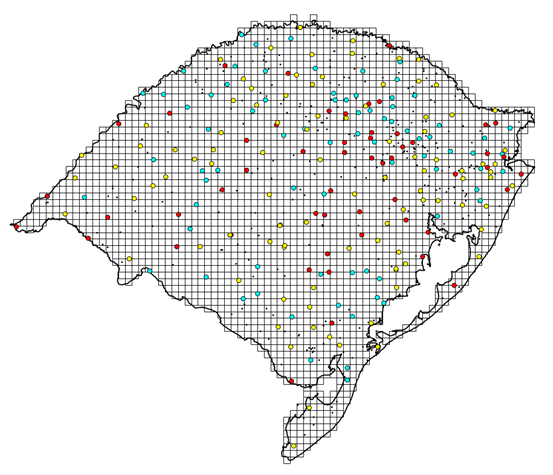
\includegraphics[width=0.7\textwidth,height=\textheight]{Figuras/Figura1a.png}

}

\subcaption{\label{fig-Figura1a}XAVIER}

\end{minipage}%
\newline
\begin{minipage}{\linewidth}

\centering{

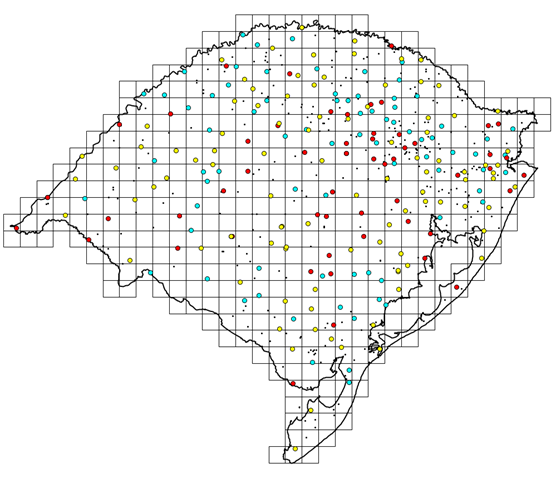
\includegraphics[width=0.7\textwidth,height=\textheight]{Figuras/Figura1b.png}

}

\subcaption{\label{fig-Figura1b}CHIRPS}

\end{minipage}%

\caption{\label{fig-Figura1}Visualização espacial da grade XAVIER (a) e
CHIRPS (b), e das estações pluviométricas. Círculos em vermelho são
estações com tamanho da série entre 25 e 30 anos, os amarelos entre 31 e
45 anos, os azuis maiores que 45 anos e os círculos pretos pequenos
indicam estações com tamanho de séries menores que 25 anos de dados.}

\end{figure}%

\subsection{Equações IDFs}\label{equauxe7uxf5es-idfs}

As relações entre a intensidade, a duração e a frequência de ocorrência
de precipitações intensas podem ser expressas por uma equação. Para
elaboração das Equações IDFs, foi utilizado o modelo de equação
tradicional, representado pela equação Equation~\ref{eq-Eq1}:

\begin{equation}\phantomsection\label{eq-Eq1}{
i=\frac{a \cdot T_{r}^{b}}{(t+c)^{d}}
}\end{equation}

Em que:

\(i\)= intensidade máxima média de chuva (mm/h);

\(a\)= fator ou parâmetroq ue determina a unidade da intensidade da
chuva;

\(T_{r}\)= tempo de retorno (anos);

\(t\)= duração da chuva (min); e

\(b\), \(c\) e \(d\) = parâmetros de ajuste dependentes da estação
pluviométrica.

A obtenção dos dados de precipitação foi feita com base nas bases de
dados apresentadas no item 2.1, elegendo-se a precipitação de maior
intensidade de cada ano. No caso das séries oriundas de estações
pluviométricas obtidas da base HIDRO, não foi realizado o preenchimento
de falhas, pois não foram considerados os anos que possuíam falhas.

A Table~\ref{tbl-Tab1} apresenta algumas curvas IDFs indicadas em
Gonçalves (2011) que foram oriundas do trabalho de Pfafstetter (1957) e
de outras relações IDF estabelecidas e publicadas para algumas regiões
do Brasil. Essas informações são importantes para possibilitar efetuar
comparações com curvas eventualmente atualizadas e aferir a ordem de
grandeza dos parametrosparâmetros obtidos.

\begin{longtable}[]{@{}
  >{\raggedright\arraybackslash}p{(\columnwidth - 12\tabcolsep) * \real{0.3514}}
  >{\raggedright\arraybackslash}p{(\columnwidth - 12\tabcolsep) * \real{0.1351}}
  >{\raggedright\arraybackslash}p{(\columnwidth - 12\tabcolsep) * \real{0.0946}}
  >{\raggedright\arraybackslash}p{(\columnwidth - 12\tabcolsep) * \real{0.1081}}
  >{\raggedright\arraybackslash}p{(\columnwidth - 12\tabcolsep) * \real{0.0946}}
  >{\raggedright\arraybackslash}p{(\columnwidth - 12\tabcolsep) * \real{0.1216}}
  >{\raggedright\arraybackslash}p{(\columnwidth - 12\tabcolsep) * \real{0.0946}}@{}}
\caption{Parâmetros das relações IDF existentes empregadas (Gonçalves,
2011). Fontes: (1)(Fragoso Jr., 2004); (2)(Bemfica et al., 2000);
(3)(Bertoni \& Tucci, 1993); (4)(Bravo et al., 2008) (5)(Distrito
Federal, 2009)}\label{tbl-Tab1}\tabularnewline
\toprule\noalign{}
\begin{minipage}[b]{\linewidth}\raggedright
LOCALIDADE
\end{minipage} & \begin{minipage}[b]{\linewidth}\raggedright
a
\end{minipage} & \begin{minipage}[b]{\linewidth}\raggedright
b
\end{minipage} & \begin{minipage}[b]{\linewidth}\raggedright
c
\end{minipage} & \begin{minipage}[b]{\linewidth}\raggedright
d
\end{minipage} & \begin{minipage}[b]{\linewidth}\raggedright
R2
\end{minipage} & \begin{minipage}[b]{\linewidth}\raggedright
FONTE
\end{minipage} \\
\midrule\noalign{}
\endfirsthead
\toprule\noalign{}
\begin{minipage}[b]{\linewidth}\raggedright
LOCALIDADE
\end{minipage} & \begin{minipage}[b]{\linewidth}\raggedright
a
\end{minipage} & \begin{minipage}[b]{\linewidth}\raggedright
b
\end{minipage} & \begin{minipage}[b]{\linewidth}\raggedright
c
\end{minipage} & \begin{minipage}[b]{\linewidth}\raggedright
d
\end{minipage} & \begin{minipage}[b]{\linewidth}\raggedright
R2
\end{minipage} & \begin{minipage}[b]{\linewidth}\raggedright
FONTE
\end{minipage} \\
\midrule\noalign{}
\endhead
\bottomrule\noalign{}
\endlastfoot
Porto Alegre (RS) & 816,598 & 0,167 & 12 & 0,760 & 0,99911 & (1) \\
Porto Alegre -- 8º DISME & 1297,900 & 0,171 & 11,619 & 0,850 & - &
(2) \\
Porto Alegre -- Aeroporto & 826,806 & 0,143 & 13,326 & 0,793 & - &
(2) \\
Cruz Alta (RS) & 1419,000 & 0,190 & 12 & 0,800 & - & (1) \\
Florianópolis (SC) & 1754,242 & 0,187 & 36 & 0,823 & 0,99869 & (1) \\
Curitiba (PR) & 998,280 & 0,178 & 9 & 0,784 & 0,99942 & (1) \\
Lins (SP) & 430,500 & 0,300 & 12 & 0,740 & - & (1) \\
Rio de Janeiro (RJ) & 1239,000 & 0,150 & 20 & 0,740 & - & (3) \\
Brasília (DF) & 1574,700 & 0,207 & 8 & 0,884 & 0,99800 & (5) \\
Aracajú (SE) & 834,205 & 0,179 & 15 & 0,726 & 0,99551 & (1) \\
Fortaleza (CE) & 1408,613 & 0,167 & 12 & 0,778 & 0,99869 & (1) \\
Teresina (PI) & 1248,856 & 0,177 & 10 & 0,769 & 0,99861 & (1) \\
São Luiz (MA) & 1519,371 & 0,161 & 28 & 0,777 & 0,99764 & (1) \\
Belém (PA) & 1085,508 & 0,156 & 12 & 0,758 & 0,99551 & (1) \\
Manaus (AM) & 1136,504 & 0,158 & 10 & 0,764 & 0,99819 & (1) \\
Porto Velho (RO) & 1182,378 & 0,159 & 11 & 0,757 & 0,99664 & (1) \\
Rio Branco (AC) & 1419,345 & 0,162 & 18 & 0,795 & 0,99779 & (1) \\
\end{longtable}

Se inexistem relações IDFs estabelecidas para o local desejado, seja
para a realização de estudos de planejamento, seja para o projeto de uma
estrutura de drenagem, o problema pode ser contornado com o emprego da
equação IDF ajustada com dados do pluviógrafo mais próximo, caso esteja
situado em região climática homogênea. Outra alternativa consiste na
utilização de métodos de desagregação de chuvas diárias (chuva acumulada
no período diário) medidas por pluviômetros na área em estudo. Neste
estudo só foram utilizados dados de chuva diária oriundos de
pluviômetros que precisaram ser desagregados para compor as chuvas para
diferentes durações.

No Brasil, a dificuldade da geração das equações para as relações IDFs
reside na baixa densidade da rede de pluviógrafos, que medem os totais
precipitados para diferentes durações (por exemplo, 5, 10, 15, 30
minutos e 1, 2 horas). Além disso, mesmo para os pluviógrafos
disponíveis os períodos de observação são relativamente curtos.Outra
dificuldade no uso dos dados de pluviógrafos reside na metodologia para
obtenção das equações de chuvas intensas que requer um exaustivo
trabalho de tabulação, análise e interpretação de grande quantidade de
pluviogramas, muitas vezes armazenados em forma de gráficos em papel, ou
seja, não digitalizados, e disponíveis apenas para consulta presencial
no órgão responsável pela guarda dos dados.

Gonçalves (2011) fez um levantamento das estações pluviográficas no
Brasil, identificou-se a época que o principal esforço realizado no
sentido de unificar e disponibilizar ao público as séries de dados
pluviográficos existentes é o Sistema Nacional de Informações sobre
Recursos Hídricos -- SNIRH, desenvolvido pela Agência Nacional de Águas
e Saneamento Básico (ANA). Gonçalves (2011) identificou que estão
armazenados dados de 372 pluviógrafos espalhados por todo o território
nacional (Table~\ref{tbl-Tab2}). Além disso, a maioria dos pluviógrafos
apresentaram séries curtas e com muitas falhas.

Além disso, a adoção de dados de pluviômetros se justifica também na
medida em que existe uma vasta rede pluviométrica instalada, como pode
ser observado na Figure~\ref{fig-Figura1}. No entanto, nos dados
pluviométricos os totais precipitados são acumulados diariamente, não
sendo registrados em menores intervalos de tempo, justamente na escala
de interesse das chuvas de grande intensidade.

\begin{longtable}[]{@{}lll@{}}
\caption{Estações pluviográficas cadastrados no SNIRH: quantidade por
bacia hidrográfica (Gonçalves, 2011).}\label{tbl-Tab2}\tabularnewline
\toprule\noalign{}
Cód. & Bacia Hidrográfica & Estações Pluviográficas \\
\midrule\noalign{}
\endfirsthead
\toprule\noalign{}
Cód. & Bacia Hidrográfica & Estações Pluviográficas \\
\midrule\noalign{}
\endhead
\bottomrule\noalign{}
\endlastfoot
1 & Rio Amazonas & 53 \\
2 & Rio Tocantins & 28 \\
3 & Atlântico - Trecho Norte/Nordeste & 25 \\
4 & Rio São Francisco & 83 \\
5 & Atlântico - Trecho Leste & 72 \\
6 & Rio Paraná & 59 \\
7 & Rio Uruguai & 37 \\
8 & Atlântico - Trecho Sudeste & 15 \\
& Total & 372 \\
\end{longtable}

Algumas metodologias que viabilizam a utilização de dados de pluviômetro
para estabelecimento da relação IDF empregam coeficientes para
transformar a chuva diária em chuvas de menor duração. Dentre elas
destaca-se o Método das Isozonas, proposto por Torrico (1974), e o
método das relações entre durações (DAE \& CETESB, 1980).

\subsection{Desagregação da
Precipitação}\label{desagregauxe7uxe3o-da-precipitauxe7uxe3o}

A desagregação de totais de chuva diária para máxima de 24 horas de
duração e em totais correspondentes para durações menores é
frequentemente realizada com os chamados coeficientes de desagregação de
chuvas. Esta prática é usada, normalmente, para estabelecer relações de
IDFs em locais que dispõem somente de dados diários medidos com
pluviômetros convencionais (Bertoni \& Tucci, 1993).

Os coeficientes de desagregação disponíveis na literatura
técnico-científica do país são apresentados na forma de tabelas e,
também, como índices em cascata (por exemplo, dois coeficientes
multiplicativos sucessivos para desagregar uma chuva de 24 horas na
chuva de 1 hora).

Várias tabelas com coeficientes de desagregação são encontradas em
diversas publicações, mas o presente estudo baseia-se naqueles
apresentados em DAE \& CETESB (1980) e Bertoni \& Tucci (1993).

Na Table~\ref{tbl-Tab3} são reproduzidos os coeficientes de desagregação
indicados em DAE \& CETESB (1980), obtidos a partir do clássico estudo
de Pfafstetter (1957), que abrangeu todo o território nacional. Os
valores dos coeficientes são relações médias de precipitação máxima com
períodos de retorno entre 2 e 100 anos obtidas das curvas IDFs propostas
por Pfafstetter (1957). Pode-se notar, um grupo de índices relativos a
durações menores que 30 min, um outro para durações iguais ou superiores
a 1 hora e um terceiro utilizado para conversão da chuva diária medida
no pluviômetro e a chuva de duração de 24 horas. O coeficiente, que
relaciona a chuva de 30 min com a chuva de 1 hora é o elo entre os dois
grupos.

Conforme a Table~\ref{tbl-Tab3}, para se obter a chuva de 5 min a partir
da chuva diária registrada no pluviômetro para um determinado tempo de
retorno, inicialmente divide-se o valor da chuva do pluviômetro por 24
h. Na sequência, aplica-se o coeficiente multiplicador de 1,13 para
converter a chuva diária em intensidade de chuva com duração de 24 hs. A
partir do valor da chuva de 24 horas, a seqüência de coeficientes em
cascata é igual a 0,42 multiplicado por 0,74 e por 0,34. Ou seja, a
chuva máxima de 5 min corresponde, com duas casas decimais, a 0,11 (ou
11\%) da chuva máxima de 24 horas ou 0,1243\% da chuva diária registrada
no pluviômetro. Pode-se estabelecer coeficientes similares para as
outras durações de chuva conforme coeficientes da Table~\ref{tbl-Tab3},
aqui denominados de coeficientes diretos de desagregação.

\begin{longtable}[]{@{}ll@{}}
\caption{Coeficientes de desagregação de chuvas (DAE \& CETESB,
1980).}\label{tbl-Tab3}\tabularnewline
\toprule\noalign{}
Relação de durações & Relação de chuvas \\
\midrule\noalign{}
\endfirsthead
\toprule\noalign{}
Relação de durações & Relação de chuvas \\
\midrule\noalign{}
\endhead
\bottomrule\noalign{}
\endlastfoot
5 min/30 min & 0,34 \\
10 min/30 min & 0,54 \\
15 min/30 min & 0,70 \\
20 min/30 min & 0,81 \\
25 min/30 min & 0,91 \\
30 min/ 1 h & 0,74 \\
1 h/ 24 h & 0,42 \\
6 h/ 24 h & 0,72 \\
8 h/ 24 h & 0,78 \\
10 h/ 24 h & 0,82 \\
12 h/ 24 h & 0,85 \\
1 dia / 24 h & 1,13 \\
\end{longtable}

\subsection{Análise de Frequência}\label{anuxe1lise-de-frequuxeancia}

A análise de frequência busca o ajuste de modelos estatísticos aos
valores máximos de variáveis hidrológicas. O primeiro objetivo da
análise de frequência é relacionar a magnitude de eventos extremos com
suas frequências de ocorrência, através do uso de distribuições de
probabilidades. Na análise de frequência são avaliados os dados
históricos da variável hidrológica disponível no local de interesse ou
por meio de regionalização.

Assim, análise de frequência de precipitações máximas envolve,
basicamente, as seguintes etapas:

\begin{enumerate}
\def\labelenumi{\alph{enumi}.}
\item
  Definição de uma amostre de precipitações máximas, na forma de uma
  série de dados. Neste estudo foram utilizadas precipitações máximas
  diárias anuais;
\item
  Essa amostra deve satisfazer os critérios estatísticos de
  aleatoriedade, independência, homogeneidade e estacionaridade, além de
  ter sido objeto de verificações de valores atípicos (outliers);
\item
  Propor uma ou algumas distribuições teóricas de probabilidade, com a
  estimativa de seus respectivos parâmetros e ajustar a melhor
  distribuição probabilística teórica aos dados, utilizando a melhor
  técnica disponível; e
\item
  Utilização da distribuição ajustada para inferir, estatisticamente, os
  valores referentes à população;
\end{enumerate}

Na análise de frequência, considera-se que os valores máximos
hidrológicos têm um comportamento aleatório, sendo necessária a
definição da distribuição de probabilidades do universo dessas
precipitações máximas. Este enfoque probabilístico permite estimar as
probabilidades de ocorrência para a magnitude dos valores máximos
hidrológicos. Para isso, utilizam-se como dados básicos, registros
históricos dessas variáveis, de onde são obtidas as amostras de máximas
ocorrências.

Quando o registro histórico é relativamente longo, a análise de
frequência de valores máximos hidrológicos pode ser feita a partir de
interpolações na curva de distribuição das frequências amostrais, que
associa probabilidades acumuladas a cada ponto da amostra ordenada, de
acordo com posições de plotagens em papéis probabilísticos. No entanto,
muito comumente, o tamanho da amostra não é suficiente para fornecer
informações a respeito de precipitações com altos períodos de retorno
(por exemplo de 100, 1.000 e 10.000 anos), sendo necessário fazer
extrapolações na curva de frequência, as quais exigem uma decisão com
grande subjetividade.

Para contornar o problema, as precipitações máximas são consideradas
como amostras de uma variável aleatória contínua, e são empregados
modelos probabilísticos devidamente ajustados a essas amostras,
permitindo que as extrapolações sejam feitas com menor subjetividade.
Esta hipótese pode, entretanto, ser bastante enganosa.

\subsubsection{Escolha da
Distribuição}\label{escolha-da-distribuiuxe7uxe3o}

A distribuição teórica tradicionalmente utilizada no ajuste de curvas
IDFs é a distribuição de Gumbel, também conhecida como Distribuição
Assintótica Tipo I. Gravatal (2024) analisou diversos trabalhos
acadêmicos sobre o tema e verificou que grande parte dos estudos, cerca
de 20 estudos no Brasil, recai sobre a distribuição de Gumbel. No
entanto, o fato de os estudos adotarem uma única distribuição, não é
evidência suficiente de que de fato essa é a distribuição mais adequada
para ajuste das IDFs.

Devido à falta de bases sólidas para a escolha da distribuição que
melhor se ajusta à série de dados, é recomendável testar diversas
distribuições (Rao \& Hamed, 2000). Essas distribuições podem ser
escolhidas, inicialmente, com base nos valores dos coeficientes de
assimetria e de curtose, através do Diagrama das Relações dos Momentos
(MRD) (Moment Ratio Diagrams em inglês) e também o L-MRD (onde L
representa uma linearização efetuada sobre os momentos), ou a partir de
distribuições recomendadas em estudos específicos como os critérios
preconizados pela ELETROBRAS (1987) no ``\emph{Guia Para Cálculo de
Cheia de Projeto de Vertedores}''.

Apesar de ser um procedimento subjetivo, o exame visual do ajuste entre
as distribuições de probabilidades candidatas e os dados observados
também pode ser útil na seleção da distribuição de probabilidades
apropriada. Embora útil, o exame visual dos dados é adequado para
amostras de grandes tamanhos, uma vez que amostras pequenas são muito
mais sensíveis à presença de erros de amostragem ou de imprecisões na
estimação da posição de plotagem, os quais podem tornar a análise visual
pouco informativa, ou até mesmo, pouco confiável.

A forma mais comum de seleção da distribuição de probabilidade é a
partir da aderência da distribuição proposta à distribuição empírica dos
valores amostrais (que compõem a série histórica). Essa aderência é
quantificada a partir de testes de hipóteses específicos, conhecidos
como testes de aderência (Chambers \& Hastie, 1992), sendo os testes do
Qui-Quadrado (Pearson, 1900) e de Komolgorov \& Smirnov (Kolmogorov,
1933; Smirnov, 1948) bastante empregados. Esses testes, embora não se
prestem a seleção de uma dentre várias distribuições possíveis, são
instrumentos da estatística que auxiliam a tomada de decisão quanto à
adequação ou inadequação de um certo modelo distributivo a uma dada
amostra. Contudo, ressalta-se que dado o baixo poder estatístico (Cohen,
1992) desses testes, o uso indiscriminado dos resultados desses testes
pode resultar em escolhas equivocadas.

\subsubsection{Estimativa dos Parâmetros da
Distribuição}\label{estimativa-dos-paruxe2metros-da-distribuiuxe7uxe3o}

Observa-se que a definição de um modelo distributivo que descreva as
características probabilísticas de um fenômeno hidrológico é um problema
complexo e passa também pela estimação dos seus parâmetros. As
distribuições frequentemente utilizadas em hidrologia apresentam um
número de parâmetros bastante variado. Apesar dos modelos de 3
parâmetros apresentarem maior flexibilidade de forma, de modo geral,
quando se dispõe de amostras curtas (com 50 valores ou menos), é
aconselhável que se investigue, primeiramente, apenas as funções que
estão definidas por um ou dois parâmetros, pois a qualidade da
estimativa é proporcional ao tamanho e à representatividade da amostra
(Burnham \& Anderson, 2002). \textbf{No presente estudo foram testas as
distribuições Gumbel (GUM) e Gama (GAM) com 2 parâmetros e a
Distribuiçãod e Extremos com Valores Generalizados (GEV) com 3
parâmetros.}

Depois de definida quais as distribuições de probabilidades que serão
analisadas, o próximo passo é a estimação dos parâmetros das
distribuições escolhidas que servirão para determinar os valores de
precipitações máximas (quantis) associados a seus respectivos períodos
de retorno. Existem inúmeros métodos de determinação dos parâmetros da
distribuição, entre os quais podemos destacar: o Método dos Momentos
(MOM) (Hansen \& Singleton, 1982), o Método da Máxima Verossimilhança
(ML) (Casella \& Berger, 2002; Cox \& Hinkley, 1961) e o Método dos
Momentos com Pesos Probabilísticos (MML) (Jørgensen, 1997; MacDonald \&
Zucchini, 2009). \textbf{No presente estudo foram testados os métodos
MOM e MML.}

O método MOM é um estimador de parâmetros relativamente simples e fácil.
Ele consiste em igualar os momentos amostrais aos populacionais. O
resultado dessa operação produzirá as estimativas dos parâmetros da
distribuição de probabilidades em questão. Embora amplamente empregado
no ajuste de curvas IDFs, o MOM tem uma qualidade inferior e menos
eficiente que outros métodos de estimação de parâmetros, como por
exemplo, o método MML (Hinkley \& Lee, 1995). Esta baixa eficiência é
notada, principalmente, quando se trata de distribuições com mais de
três parâmetros, pois os momentos de ordem alta têm uma probabilidade
maior de estarem enviesado em amostras relativamente pequenas (Johnson
\& Kotz, 1994).

O método MML em geral resulta em uma estimativa com procedimentos de
cálculos mais simples. A estimativa dos parâmetros pelo MML apresenta,
em alguns casos, valores mais precisos quando comparado a outros
métodos, como o método da Mínima Variância Assintótica (MVS), por
exemplo (Morrison \& Tang, 1994). A estimação dos parâmetros pelo MML é
obtida de maneira análoga ao MOM, igualando cada momento com peso
probabilístico teórico com sua estimativa amostral, formando um sistema
de equações cujas incógnitas são os parâmetros da distribuição teórica.
O MML apresenta-se como uma técnica eficiente para estimativa dos
parâmetros de uma distribuição de probabilidades.

\textbf{Neste estudo foram testados 3 modelos probabilísticos: as
distribuições Gumbel (GUM) e Gama (GAM) com 2 parâmetros e a Extremos
Valores Generalizados (GEV) com 3 parâmetros. Para estimar esses
parâmetros foram utilizados os métodos MOM e MML.}

\subsection{Período de Retorno}\label{peruxedodo-de-retorno}

O período de retorno é o intervalo de tempo médio entre a ocorrência de
uma determinada magnitude ou intensidade, com base em uma série
histórica de observações. Matematicamente corresponde ao inverso da
probabilidade de um determinado evento (chuva ou vazão) de ser igualado
ou excedido em um ano qualquer.

Ao decidir se uma estrutura hidráulica será projetada para uma chuva ou
vazão com período de retorno de \(T_{r}\) anos, automaticamente,
decide-se o grau de proteção conferido à população, uma vez que se
define qual é o ``risco aceitável'', ou seja, a probabilidade de uma
determinada estrutura hidráulica vir a falhar pelo menos uma vez durante
sua vida útil.

Esse conceito leva em conta que uma estrutura hidráulica projetada para
um período de retorno \(T_{r}\) expõe-se, todo o ano, a uma
probabilidade \(1/T_{r}\) de vir a falhar. É intuitivo que, ao longo de
\(n\) anos de sua vida útil, essa obra terá um risco de falha maior do
que \(1/T_{r}\), uma vez que ficará exposta, repetidamente, a essa
possibilidade.

A expressão para o cálculo do risco \(R\), deduzida da teoria das
probabilidades é, portanto, função do tempo de retorno \(T_{r}\) e do
número de anos esperado para a vida útil da estrutura e é representada
por:

\begin{equation}\phantomsection\label{eq-Eq2}{
R=100\cdot\bigg[1- \bigg(1-\frac{1}{T_r}\bigg)\bigg]^{n}
}\end{equation}

Em que:

\(R\)= Risco (\%);

\(T_{r}\)= Período de retorno (anos); e

\(n\)= vida útil (anos).

Algumas referências para tempos de retorno utilizados para estruturas
hidráulicas destinadas à drenagem urbana são apresentados na
Table~\ref{tbl-Tab4}.

\begin{longtable}[]{@{}
  >{\raggedright\arraybackslash}p{(\columnwidth - 4\tabcolsep) * \real{0.2361}}
  >{\raggedright\arraybackslash}p{(\columnwidth - 4\tabcolsep) * \real{0.5278}}
  >{\raggedright\arraybackslash}p{(\columnwidth - 4\tabcolsep) * \real{0.2361}}@{}}
\caption{Período de retorno para diferentes ocupações de área (Porto,
1995).}\label{tbl-Tab4}\tabularnewline
\toprule\noalign{}
\begin{minipage}[b]{\linewidth}\raggedright
Tipo de Drenagem
\end{minipage} & \begin{minipage}[b]{\linewidth}\raggedright
Tipo de Ocupação da Área/Obra
\end{minipage} & \begin{minipage}[b]{\linewidth}\raggedright
Tempo de Retorno (anos)
\end{minipage} \\
\midrule\noalign{}
\endfirsthead
\toprule\noalign{}
\begin{minipage}[b]{\linewidth}\raggedright
Tipo de Drenagem
\end{minipage} & \begin{minipage}[b]{\linewidth}\raggedright
Tipo de Ocupação da Área/Obra
\end{minipage} & \begin{minipage}[b]{\linewidth}\raggedright
Tempo de Retorno (anos)
\end{minipage} \\
\midrule\noalign{}
\endhead
\bottomrule\noalign{}
\endlastfoot
Microdrenagem & Residencial & 2 \\
Microdrenagem & Comercial & 5 \\
Microdrenagem & Áreas com edifícios de serviços públicos & 5 \\
Microdrenagem & Aeroportos & 2-5 \\
Microdrenagem & Áreas comerciais e artérias de tráfego & 5-10 \\
Microdrenagem & Áreas comerciais e residenciais & 50-100 \\
Macrodrenagem & Áreas de importância e específica & 500- \\
\end{longtable}

A Table~\ref{tbl-Tab5} correlaciona o período de retorno e a vida útil
da obra apresentando o risco percentual associado à falha, conforme
Equation~\ref{eq-Eq1}.

\begin{longtable}[]{@{}
  >{\raggedright\arraybackslash}p{(\columnwidth - 10\tabcolsep) * \real{0.1667}}
  >{\raggedright\arraybackslash}p{(\columnwidth - 10\tabcolsep) * \real{0.1667}}
  >{\raggedright\arraybackslash}p{(\columnwidth - 10\tabcolsep) * \real{0.1667}}
  >{\raggedright\arraybackslash}p{(\columnwidth - 10\tabcolsep) * \real{0.1667}}
  >{\raggedright\arraybackslash}p{(\columnwidth - 10\tabcolsep) * \real{0.1667}}
  >{\raggedright\arraybackslash}p{(\columnwidth - 10\tabcolsep) * \real{0.1667}}@{}}
\caption{Riscos percentuais de falha em função do período de retorno e
vida útil da obra.}\label{tbl-Tab5}\tabularnewline
\toprule\noalign{}
\begin{minipage}[b]{\linewidth}\raggedright
Tempo de Retorno (anos)/Vida Útil (anos)
\end{minipage} & \begin{minipage}[b]{\linewidth}\raggedright
2
\end{minipage} & \begin{minipage}[b]{\linewidth}\raggedright
5
\end{minipage} & \begin{minipage}[b]{\linewidth}\raggedright
25
\end{minipage} & \begin{minipage}[b]{\linewidth}\raggedright
50
\end{minipage} & \begin{minipage}[b]{\linewidth}\raggedright
100
\end{minipage} \\
\midrule\noalign{}
\endfirsthead
\toprule\noalign{}
\begin{minipage}[b]{\linewidth}\raggedright
Tempo de Retorno (anos)/Vida Útil (anos)
\end{minipage} & \begin{minipage}[b]{\linewidth}\raggedright
2
\end{minipage} & \begin{minipage}[b]{\linewidth}\raggedright
5
\end{minipage} & \begin{minipage}[b]{\linewidth}\raggedright
25
\end{minipage} & \begin{minipage}[b]{\linewidth}\raggedright
50
\end{minipage} & \begin{minipage}[b]{\linewidth}\raggedright
100
\end{minipage} \\
\midrule\noalign{}
\endhead
\bottomrule\noalign{}
\endlastfoot
2 & 75 & 96.88 & 100 & 100 & 100 \\
5 & 36 & 67.23 & 99.62 & 100 & 100 \\
10 & 19 & 40.95 & 92.82 & 99.48 & 100 \\
25 & 7.84 & 18.46 & 63.96 & 87.01 & 98.31 \\
50 & 3.96 & 9.61 & 39.65 & 63.58 & 86.74 \\
100 & 1.99 & 4.9 & 22.22 & 39.5 & 63.4 \\
500 & 0.4 & 1 & 4.88 & 9.53 & 18.14 \\
\end{longtable}

Como exemplo, considere que uma determinada estrutura hidráulica tenha
vida útil de 50 anos. O risco desta estrutura vir a falhar, pelo menos
uma vez, durante sua vida útil, é de praticamente 100\%, quando o
período de retorno é igual a 2 e 5 anos, 99\% para quando igual a 10
anos, 87\% quando 25 anos, 64\% quando 50 anos, 39\% quando igual a 100
anos e 9\% quando igual a 500 anos.

A American Society of Civil Engineers (1992) recomenda que a escolha do
período de retorno deva ser precedida de um estudo de risco associado
aos danos provocados por um evento hidrológico superior ao de projeto
durante a vida útil da estrutura hidráulica. Diante deste critério,
devem ser avaliados: o porte da obra, a densidade de população da
região, o volume de tráfego do sistema viário do local, o entorno da
região, proximidade de escolas, hospitais, estádios, estações
ferroviárias ou de metrô, terminais de ônibus, aeroportos, etc. Esse
critério deve ser definido politicamente, uma vez que a população e os
seus representantes governamentais decidirão o grau de proteção
desejável e o quanto estarão dispostos a pagar por ele.

Para Tucci (2004), existem certas dificuldades em se estabelecer o
período de retorno objetivamente. Estas dificuldades estão ligadas a
aspectos políticos, sociais, econômicos e hidrológicos. Estudos
econômicos, como uma análise custo-benefício, poderiam orientar essa
escolha. Mas, a necessidade de se considerar custos e benefícios de
difícil quantificação e, ainda mais, a impossibilidade de se levar em
conta uma série de aspectos que não podem ser expressos em termos
monetários, limitam a aplicação desta metodologia.

\subsection{Estimativa dos parâmetros a, b, c e d das relações
IDFs}\label{estimativa-dos-paruxe2metros-a-b-c-e-d-das-relauxe7uxf5es-idfs}

Para o cálculo das chuvas extremas, procedeu-se a estimativa dos
parâmetros de curvas IDFs para todas as séries de dados, a partir das
três bases consideradas, HIDRO, XAVIER e CHIRPS.

Para a automatização da geração das curvas IDFs para todas as séries,
foi implementado um programa em linguagem JAVA no âmbito do sistema
FERAH, que realiza, de forma iterativa para todas as séries, as
seguintes etapas:

\begin{enumerate}
\def\labelenumi{\alph{enumi}.}
\item
  Leitura das séries de chuva diária de determinada base de dados
  (HIDRO, XAVIER, ou HIDRO);
\item
  Organização da série de precipitação diária máxima por ano
  hidrológico;
\item
  Análise de frequência da série de precipitação diária máxima por ano
  hidrológico, considerando a abordagem apresentada no item 2.4; e
\item
  Desagregação das precipitações diárias associadas a diferentes tempos
  de retorno por meio dos coeficientes de desagregação apresentados na
  Table~\ref{tbl-Tab3}. Inicialmente, procede-se com a desagregação da
  chuva diária medida no pluviômetro para chuva de duração de 24 horas,
  por meio do respectivo coeficiente de desagregação. Em seguida, as
  precipitações de 24 horas são desagregadas em alturas de chuva de
  menor duração (12 h, 9h, 6h, 3h, 2h, 1 h, 30 min, 25 min, 15 min, 10
  min e 5 min);
\item
  Definição dos parâmetros da equação que representa as relações IDFs
  estabelecidas com a desagregação de chuvas;
\item
  Escrita dos resultados em arquivos de saída.
\end{enumerate}

Para a implementação da etapa (e), foi utilizada a mesma abordagem
adotada em Gonçalves (2011). Assim, a equação geral da curva IDF
(Equation~\ref{eq-Eq2}) foi linearizada com o uso de logaritmos, da
seguinte forma:

\begin{equation}\phantomsection\label{eq-Eq3}{
log(i)=log(a) + b\cdot log(T_r) - d\cdot log(t+c)
}\end{equation}

Denominando-se, \(Y=log(i)\); \(X1=log(T_r)\); \(X2=log(t+c)\) e
\(A=log(a)\), tem-se:

\begin{equation}\phantomsection\label{eq-Eq4}{
Y=A + bX1 + dX2
}\end{equation}

que é uma equação linear de duas variáveis (\(X1\) e \(X2\)), cujos
parâmetros \(A\), \(b\) e \(d\) podem ser obtidos por regressão
múltipla.

Já o parâmetro \(c\) não pode ser explicitado no logaritmo, de forma que
sua obtenção foi feita de forma iterativa: uma vez que os valores
característicos deste parâmetro se situam entre 0 e 30, o programa
realiza 600 ajustes, variando o valor de c entre -30 e +30, com passo de
0,1. O valor final de \(c\) é aquele que resulta no maior valor do
coeficiente de determinação R2.

\subsection{Espacialização e comparação das intensidades das chuvas
máximas}\label{espacializauxe7uxe3o-e-comparauxe7uxe3o-das-intensidades-das-chuvas-muxe1ximas}

Para a comparação do comportamento espacial das chuvas entre as
diferentes bases de dados (HIDRO, XAVIER E CHIRPS), após o ajuste das
equações IDFs, conforme descrito no item 2.6, por simplificação,
optou-se por adotar a intensidade da chuva com duração de 24 horas,
incluindo os tempos de retorno de 2, 5, 25, 100 e 500 anos como
referencial de comparação.

Após o cálculo dos parâmetros das curvas IDFs para todas as diferentes
bases de dados, foi implementado um algoritmo em linguagem R
(R-Core-Team, 2023) para cálculo das intensidades de precipitações com
os diferentes tempos de retorno supramencionados para a duração de chuva
de 24 horas, considerando os tempos de retorno descritos e as diferentes
bases de dados consideradas.

Como para base HIDRO obtem-se uma equação IDF para cada estação
pluviométrica e para as bases em grade (XAVIER e CHIRPS) são obtidas uma
equação IDF para cada ponto de grade, duas abordagens foram utilizadas
para a comparação dos padrões de intensidade de chuvas geradas pelas
diferentes IDFs. A primeira abordagem, denominada abordagem de
comparação localizada (ABL), consistiu em uma comparação pontual nos
locais das próprias estações pluviométricas. A segunda abordagem,
denominada abordagem de comparação espacializada (ABE), consistiu em uma
comparação espacial ao longo de toda a área de estudo cobrindo todos os
pontos de grade. Essas comparações visaram avaliar as diferenças
espaciais nas intensidades de chuvas dos dados provenientes diretamente
das bases em grade e aqueles que seriam obtidos por interpolação direta
a partir das estações pluviométricas para os pontos equivalentes das
grades dessas bases.

Outra avaliação realizada consistiu em comparar os resultados da
espacialização das intensidades de chuva obtidas de duas formas. A
primeira, a partir da espacialização das intensidades de chuva de 24
horas obtidas a partir das equações IDFs para cada estação pluviométrica
e, posteriormente, espacializadas por um método de interpolação para as
células de grade. A segunda forma consistiu em primeiro espacializar os
parâmetros das equações IDFs ajustadas a partir das estações para as
células da grade. Com os parâmetros das IDFs interpolados para cada
célula de grade, procedeu-se com o cálculo da intensidade da chuva de 24
horas para os diferentes tempos de retorno. Esta avaliação foi realizada
apenas pelo método IDW considerando as células da base XAVIER.

\subsubsection{Abordagem de comparação localizada
(ABL)}\label{abordagem-de-comparauxe7uxe3o-localizada-abl}

A ABL buscou comparar, na própria localidade das estações
pluviométricas, os valores das intensidades de chuvas de 24 horas para
diferentes tempos de retorno, provenientes das três bases avaliadas. Ou
seja, a abordagem visou verificar o quão bem as bases em grade (XAVIER e
CHIRPS) reproduzem os padrões de intensidade de chuvas das IDFs geradas
diretamente a partir dos dados locais das estações pluviométricas (base
HIDRO). Para isso, foi implementado um algoritmo em linguagem R que
identificou, para cada uma das bases XAVIER e CHIRPS, as células das
grades que continham estações pluviométricas da base HIDRO. Assim, as
intensidades de chuvas com duração de 24 horas para os tempos de retorno
de interesse, obtidas a partir das equações IDFs ajustadas, foram
comparadas nesses pontos de grade coincidentes com as estações
pluviométricas.

\subsubsection{Abordagem de comparação espacial
(ABE)}\label{abordagem-de-comparauxe7uxe3o-espacial-abe}

A ABE buscou espacializar as intensidades da chuvas de 24 horas para os
diferentes tempos de retorno das estações para os pontos de grade
correspondentes àqueles das bases XAVIER e CHIRPS. A partir disso, foi
comparado o comportamento espacial das intensidades de chuvas de 24
horas para os diferentes tempos de retorno, interpoladas nos pontos de
grade a partir dos dados das estações da base HIDRO. Os pontos de grade
considerados foram os mesmos das bases XAVIER e CHIRPS. Assim,
comparou-se a espacialização da chuva de referência, transportada para
os pontos de grade a partir dos dados das estações, com aqueles obtidos
diretamente das bases XAVIER e CHIRPS em toda a área de estudo.

A interpolação (ou espacialização) dos dados das estações pluviométricas
para os pontos de grade foi realizada a partir de duas técnicas: a
interpolação ponderada pelo inverso da distância ou \emph{Inverse
Distance Weighting} (IDW) e krigagem ordinária (OK).

\paragraph{Espacialização por interpolação ponderada pelo inverso da
distância
(IDW)}\label{espacializauxe7uxe3o-por-interpolauxe7uxe3o-ponderada-pelo-inverso-da-distuxe2ncia-idw}

O método IDW é uma técnica amplamente utilizada para estimar valores
desconhecidos em pontos com base em dados amostrais próximos. O método
foi inicialmente descrito por Shepard (1968) e a ideia principal é que
pontos mais próximos têm uma maior influência na estimativa do que
pontos mais distantes.

A fórmula para calcular o valor estimado de intensidade de chuva
\(\hat i_{24}^{T_r} (x_0)\) com duração de 24 hs para cada valor de
\(T_r\) em um ponto \(x_0\) é dada por:

\begin{equation}\phantomsection\label{eq-Eq5}{
\hat i_{24}^{T_r} (x_0) = \frac{\sum_{i=1}^{n} w_{x_i} \cdot i_{24}^{T_r} (x_i)}{\sum_{i=1}^{n} w_{x_i}}
}\end{equation}

em que:

\(\hat i_{24}^{T_r} (x_0)\)= valor de intensidade de chuva com duração
de 24 horas e tempo de retorno \(T_r\), estimado no ponto de valor
desconhecido \(x_0\);

\(w_{x_i}\)= peso associado ao ponto \(x_i\), calculado como
\(w_{x_i} = \frac{1}{d(x_i,x_0)^p}\);

\(d(x_i,x_0)\)= distância entre o ponto \(x_i\) e o ponto \(x_0\);

\(i_{24}^{T_r} (x_i)\)= intensidade de chuva com duração de 24 horas e
tempo de retorno \(T_r\), observado no ponto \(x_i\); e

\(p\)= parâmetro de potência que controla a influência da distância nos
pesos.

O parâmetro de potência \(p\) tem total influência nos valores dos pesos
adotados na ponderação e, consequentemente, nos resultados da
interpolação. Para se considerar o melhor valor foi realizada uma
análise de sensibilidade e otimização deste parâmetro por meio de um
processo de avaliação multicretério onde, após a análise de
sensibilidade, foi definido o valor de \(p\) que minimizasse o erro
quadrado médio (RMSE) e a diferença percentual entre os coeficientes
angulares da reta 1:1 e da reta de ajuste linear entre valores
observados e preditos (\% \(\Delta\)\(\alpha\)).

Dessa forma, para cada valor de \(T_r\) considerado (2, 5, 25, 100 e 500
anos) foi definido o melhor parâmetro \(p\).

\paragraph{Espacialização por krigagem ordinária
(OK)}\label{espacializauxe7uxe3o-por-krigagem-ordinuxe1ria-ok}

A OK também consiste em um método de interpolação, contudo, possui um
embasamento estatístico. O modelo de OK utiliza uma função de variograma
para modelar a estrutura espacial dos dados. Na OK como também se assume
que a soma dos pesos deve ser unitária, a média é estimada localmente e
não se faz necessário conhecer a média da distribuição global dos dados.
Assim a OK relaxa a hipótese de estacionariedade da média global fazendo
uso das informações localizadas dos dados. A OK é amplamente utilizada
em geostatística para criar superfícies contínuas a partir de dados
pontuais. O objetivo é encontrar a estimativa mais precisa de um valor
desconhecido minimizando a variância do erro de estimativa. A fórmula
geral para a estimativa de OK é dada por:

\begin{equation}\phantomsection\label{eq-Eq6}{
\hat i_{24}^{T_r} (x_0) = \sum_{i=1}^{n} \lambda_{x_i} \cdot i_{24}^{T_r} (x_i)
}\end{equation}

onde:

\(\hat i_{24}^{T_r} (x_0)\)= valor de intensidade de chuva com duração
de 24 horas e tempo de retorno \(T_r\), estimado no ponto de valor
desconhecido \(x_0\);

\(\lambda_{i_{24}^{T_r}(x_i)}\)= pesos atribuídos a cada ponto amostral
\(x_i\); e

\(i_{24}^{T_r} (x_i)\)= intensidade de chuva com duração de 24 horas e
tempo de retorno \(T_r\) observado no ponto \(x_i\).

Embora do ponto de vista estrutural a Equation~\ref{eq-Eq6} seja similar
àquela adotada no método IDW (Equation~\ref{eq-Eq5}), a diferença
fundamental encontra-se na forma como os pesos são calculados. Ao
contrário do método IDW, a OK consiste em um modelo estatístico de tal
forma que os pesos \(\lambda_{i_{24}^{T_r}(x_i)}\) são calculados
resolvendo-se um sistema de equações que minimiza a variância do erro de
estimação baseado no variograma empírico dos dados. Portanto, o sistema
de equações linear a ser resolvido incorpora a covariância existente na
estrutura de dados e é dado por:

\[
\begin{bmatrix}
Cov\bigg(i_{24}^{T_r}(x_1), i_{24}^{T_r}(x_1)\bigg) & Cov\bigg(i_{24}^{T_r}(x_1), i_{24}^{T_r}(x_2)\bigg) & \cdots & Cov\bigg(i_{24}^{T_r}(x_1), i_{24}^{T_r}(x_n)\bigg) & 1 \\
Cov\bigg(i_{24}^{T_r}(x_2), i_{24}^{T_r}(x_1)\bigg) & Cov\bigg(i_{24}^{T_r}(x_2), i_{24}^{T_r}(x_2)\bigg) & \cdots & Cov\bigg(i_{24}^{T_r}(x_2), i_{24}^{T_r}(x_n)\bigg) & 1 \\
\vdots & \vdots & \ddots & \vdots & \vdots \\
Cov\bigg(i_{24}^{T_r}(x_n), i_{24}^{T_r}(x_1)\bigg) & Cov\bigg(i_{24}^{T_r}(x_n), i_{24}^{T_r}(x_2)\bigg) & \cdots & Cov\bigg(i_{24}^{T_r}(x_n), i_{24}^{T_r}(x_n)\bigg) & 1 \\
1 & 1 & \cdots & 1 & 0
\end{bmatrix}
\begin{bmatrix}
\lambda_{i_{24}^{T_r}(x_1)} \\
\lambda_{i_{24}^{T_r}(x_2)} \\
\vdots \\
\lambda_{i_{24}^{T_r}(x_n)} \\
\mu
\end{bmatrix}
=
\] \begin{equation}\phantomsection\label{eq-Eq7}{
\begin{bmatrix}
Cov\bigg(i_{24}^{T_r}(x_1), i_{24}^{T_r}(x_0)\bigg) \\
Cov\bigg(i_{24}^{T_r}(x_2), i_{24}^{T_r}(x_0)\bigg) \\
\vdots \\
Cov\bigg(i_{24}^{T_r}(x_n), i_{24}^{T_r}(x_0)\bigg) \\
1
\end{bmatrix}
}\end{equation}

em que:

\(Cov(.)\)= covariância; e

\(\mu\)= parâmetro necessário para garantir que a soma dos pesos
\(\lambda_{i_{24}^{T_r}(x_i)}\) sejam unitários.

Este sistema de quações pode ser reescrito de forma simplificada como:

\begin{equation}\phantomsection\label{eq-Eq8}{
\begin{bmatrix}
\mathbf{C} & \mathbf{1} \\
\mathbf{1}^T & 0
\end{bmatrix}
\begin{bmatrix}
\boldsymbol{\lambda} \\
\mu
\end{bmatrix}
=
\begin{bmatrix}
\mathbf{c}_0 \\
1
\end{bmatrix}
}\end{equation}

Em que:

\(\mathbf{C}\) é a matriz de covariância \(n\) X \(n\) com os elementos
\(Cov\bigg(i_{24}^{T_r}(x_i), i_{24}^{T_r}(x_j)\bigg)\);

\(\mathbf{1}\) é um vetor coluna de tamanho \(n\) com todos os elementos
iguais a 1;

\(\mathbf{1^T}\) é o vetor linha de tamanho \(n\) com todos os elementos
iguais a 1;

\(\mathbf{\lambda}\) é o vetor coluna com os pesos;

\(\mathbf{\mu}\) é parâmetro que garante a unidade na soma dos pesos; e

\(\mathbf{c_0}\) é o vetor coluna com elementos
\(Cov\bigg(i_{24}^{T_r}(x_i), i_{24}^{T_r}(x_0)\bigg)\).

A OK considera a proximidade entre os dados a partir de
\(\mathbf{c_0}\), a redundância de dados a partir de \(\mathbf{C}\) e o
variograma dos dados. Embora a krigagem traga uma certa sofisticação
estatística na forma de realizar a interpolação, esta abordagem não
necessariamente implica em melhores resultados de interpolação quando
empregada para mapear a distribuição espacial de atributos que não
tenham a sua variabilidade no espaço distribuída de forma mais suave.
Neste caso, pode ser necessário o emprego de outras formas de se definir
os pesos do vetor \(\mathbf{\lambda}\), por meio da inclusão de outras
covariáveis de interesse. Contudo, isto não foi objeto deste estudo.
Maiores detalhes a respeito da OK são detalahdos em Matheron (1963).

Para este estudo, foram testados diferentes tipos de funções de
variograma (linear, hiperbólico, exponencial e gaussiano), tendo-se
optado por adotar o modelo gaussiano. Após sucessivas análises de
performance, adotou-se para os parâmetros do modelo de variograma
gaussiano o alcance de 50000, nugget =0.12 e sill=0.8.

\subsection{Incertezas entre os modelos de distribuições e métodos de
estimativa de
parâmetros}\label{incertezas-entre-os-modelos-de-distribuiuxe7uxf5es-e-muxe9todos-de-estimativa-de-paruxe2metros}

Considerando os diferentes modelos de distribuições de valores máximos
testados (GUM, GAM e GEV) e os dois métodos para a estimativa dos
parâmetros das distribuições avaliados (MOM e MML), buscou-se realizar
uma análise das incertezas associadas a essas diferentes distribuições e
metodologias de forma espacializada nas estações pluviométricas da base
HIDRO. Para isso após o cálculo da chuva máxima com duração de 24 horas
para os diferentes tempos de recorrência considerados e todas as
distribuições e métodos de estimativa de parâmetros, calculou-se a
diferença percentual entre os valores máximos e mínimos obtidos em todas
as estações consideradas.

\subsection{Estimativa do erro entre as bases de dados em grade e as
estações
pluviométricas}\label{estimativa-do-erro-entre-as-bases-de-dados-em-grade-e-as-estauxe7uxf5es-pluviomuxe9tricas}

Partindo-se da premissa que a intensidade de chuva de 24 horas estimada
a partir das estações da base HIDRO consistiria no valor de referência
em cada estação, computou-se a diferença entre aqueles valores de
intensidade de chuva de 24 horas obtidos nos pontos de grade
coincidentes com as estações pluviométricas para as bases XAVIER e
CHIRPS com os correspondentes valores obtidos a partir dos dados das
estações para os diferentes tempos de retorno.

\subsection{Análise de performance e comparação dos
resultados}\label{anuxe1lise-de-performance-e-comparauxe7uxe3o-dos-resultados}

Para comparação dos resultados obtidos a partir das diferentes bases,
análise de sensibildiade e escolha da técnica de interpolação mais
adequada entre aquelas testadas, foram utilizadas algumas métricas e
procedimentos específicos para tornar mais objetivo este processo.

\subsubsection{\texorpdfstring{Erro quadrado médio
(\(RMSE\))}{Erro quadrado médio (RMSE)}}\label{erro-quadrado-muxe9dio-rmse}

O Erro Quadrático Médio (\(RMSE\)) é uma métrica de avaliação que mede a
precisão de um modelo de previsão, calculando a raiz quadrada da média
dos quadrados das diferenças entre os valores previstos e os valores
reais. Ele fornece uma medida da magnitude média dos erros de previsão
em unidades da variável de interesse e é dado por:

\begin{equation}\phantomsection\label{eq-Eq9}{
RMSE = \sqrt{\frac{1}{n} \sum_{i=1}^{n} (y_i - \hat{y}_i)^2}
}\end{equation}

Em que:

\(n\)= número total de observações;

\(y_i\)= valor da \(i\)-ésima observação; e

\(\hat{y}_i\)= valor previsto para a \(i\)-ésima observação.

Valores menores de \(RMSE\) indicam que as previsões do modelo estão
mais próximas dos valores reais, o que reflete uma melhor precisão do
modelo. Valores maiores indicam que há uma maior discrepância entre os
valores previstos e os valores reais, o que sugere uma menor precisão do
modelo.

\subsubsection{Erro percentual absoluto médio
(MAPAE)}\label{erro-percentual-absoluto-muxe9dio-mapae}

O Erro Percentual Absoluto Médio (MAPE) também é uma métrica usada para
avaliar a precisão de modelos de previsão, contudo considerada a média
dos erros percentuais absolutos entre os valores previstos e os valores
reais. Ela fornece uma visão percentual da magnitude média dos erros de
previsão. A expressão para o cálculo do MAPE é dada por:

\begin{equation}\phantomsection\label{eq-Eq10}{
MAPE = \frac{1}{n} \sum_{i=1}^{n} \left| \frac{y_i - \hat{y}_i}{y_i} \right| \times 100
}\end{equation} Valores menores de \(MAPE\) indicam que as previsões do
modelo estão mais próximas dos valores reais, em termos percentuais, o
que sugere uma melhor precisão do modelo. Valores maiores indicam que há
uma maior discrepância entre os valores previstos e os valores reais, o
que sugere uma menor precisão do modelo.O MAPE é útil porque fornece uma
medida de erro percentual, o que facilita a comparação entre modelos e
entre diferentes conjuntos de dados, independentemente da unidade de
medida.

\subsubsection{Leave-One-Out/Cross-Validation
(LOOCV)}\label{leave-one-outcross-validation-loocv}

O método LOOVC é uma técnica de validação cruzada utilizada para avaliar
a performance de um modelo de predição. Neste estudo esta técnica foi
utilizada para avaliar a performance do método \(IDW\) para diferentes
valores do parâmetro \(p\) e, também, para comparar a performance entre
os diferentes métodos de interpolação. Partindo-se dos pontos onde há
medições (estações pluviométricas), em cada iteração, um único ponto de
dados é utilizado como conjunto de teste, enquanto o restante dos dados
é utilizado como conjunto de treinamento. O processo é repetido para
cada ponto de dados, resultando em uma predição para cada observação
individual. Ou seja, para cada ponto de dados i, o ponto é excluído do
conjunto de treinamento e usado como conjunto de teste. O modelo de
interesse é então aplicadado para prever o valor do ponto de teste, com
base no conjunto de treinamento. Após concluir o processo LOOCV, uma das
métricas (\(RMSE\) ou \(MAPE\)) pode ser empregada para comparar os
valores previstos e observados.

Portanto, o LOOVC avalia o desempenho de um modelo de predição excluindo
um ponto de dados de cada vez e treinando o modelo com o restante dos
dados. A métrica de erro é então calculada para cada ponto excluído, e o
processo fornece uma avaliação completa do modelo.

\section{Resultados e Discussões}\label{resultados-e-discussuxf5es}

\justifying

\subsection{Avaliação da ABL}\label{avaliauxe7uxe3o-da-abl}

Conforme descrito na metodologia, a ABL teve como objetivo avaliar a
eficácia das bases em grade (XAVIER e CHIRPS) na reprodução dos padrões
de intensidade de chuvas das IDFs, que foram geradas diretamente a
partir dos dados locais das estações pluviométricas (base HIDRO).
Portanto, a primeira análise consistiu em identificar as células dos
pontos de grade de cada uma dessas bases que coincidiam com os pontos
das estações da base HIDRO e, para essas células, realizar as
comparações das intensidades de chuvas de 24 h de duração para os tempos
de retorno \(T_r=(2, 5, 25, 100\ e \ 500 \ anos)\). Por praticidade,
foram apresentados os resultados apenas para a distrbuição GEV com os
parâmetros definidos pelo método MML.

A Figure~\ref{fig-Figura2a} mostra as célculas de grid da base de dados
XAVIER que foram selecionadas e consideradas representativas das
estaçoes pluviométricas. Para locais em que a estação não estava contida
exatamente dentro dos limites de uma célula, foi considerada a célula de
grid mais próxima como representativa. A base de dados XAVIER apresenta
uma resolução espacial menor (as células de grid correspondem a cerca de
10 km X 10 km). Ao todo, dos 2.572 elementos de grid, 224 foram
selecionados para representar 229 pontos de estações pluviométricas.

De forma similar, a Figure~\ref{fig-Figura2b} mostra as célculas de grid
da base de dados CHIRPS que foram selecionadas e consideradas
representativas das estaçoes pluviométricas. Para esta base de dados, a
resolução espacial é maior (as células de grid correspondem a cerca de
25 km X 25 km) totalizando 475 elementos de grid. Desses, 187 foram
selecionados para representar os 229 pontos de estações pluviométricas.

\begin{figure}

\begin{minipage}{\linewidth}

\centering{

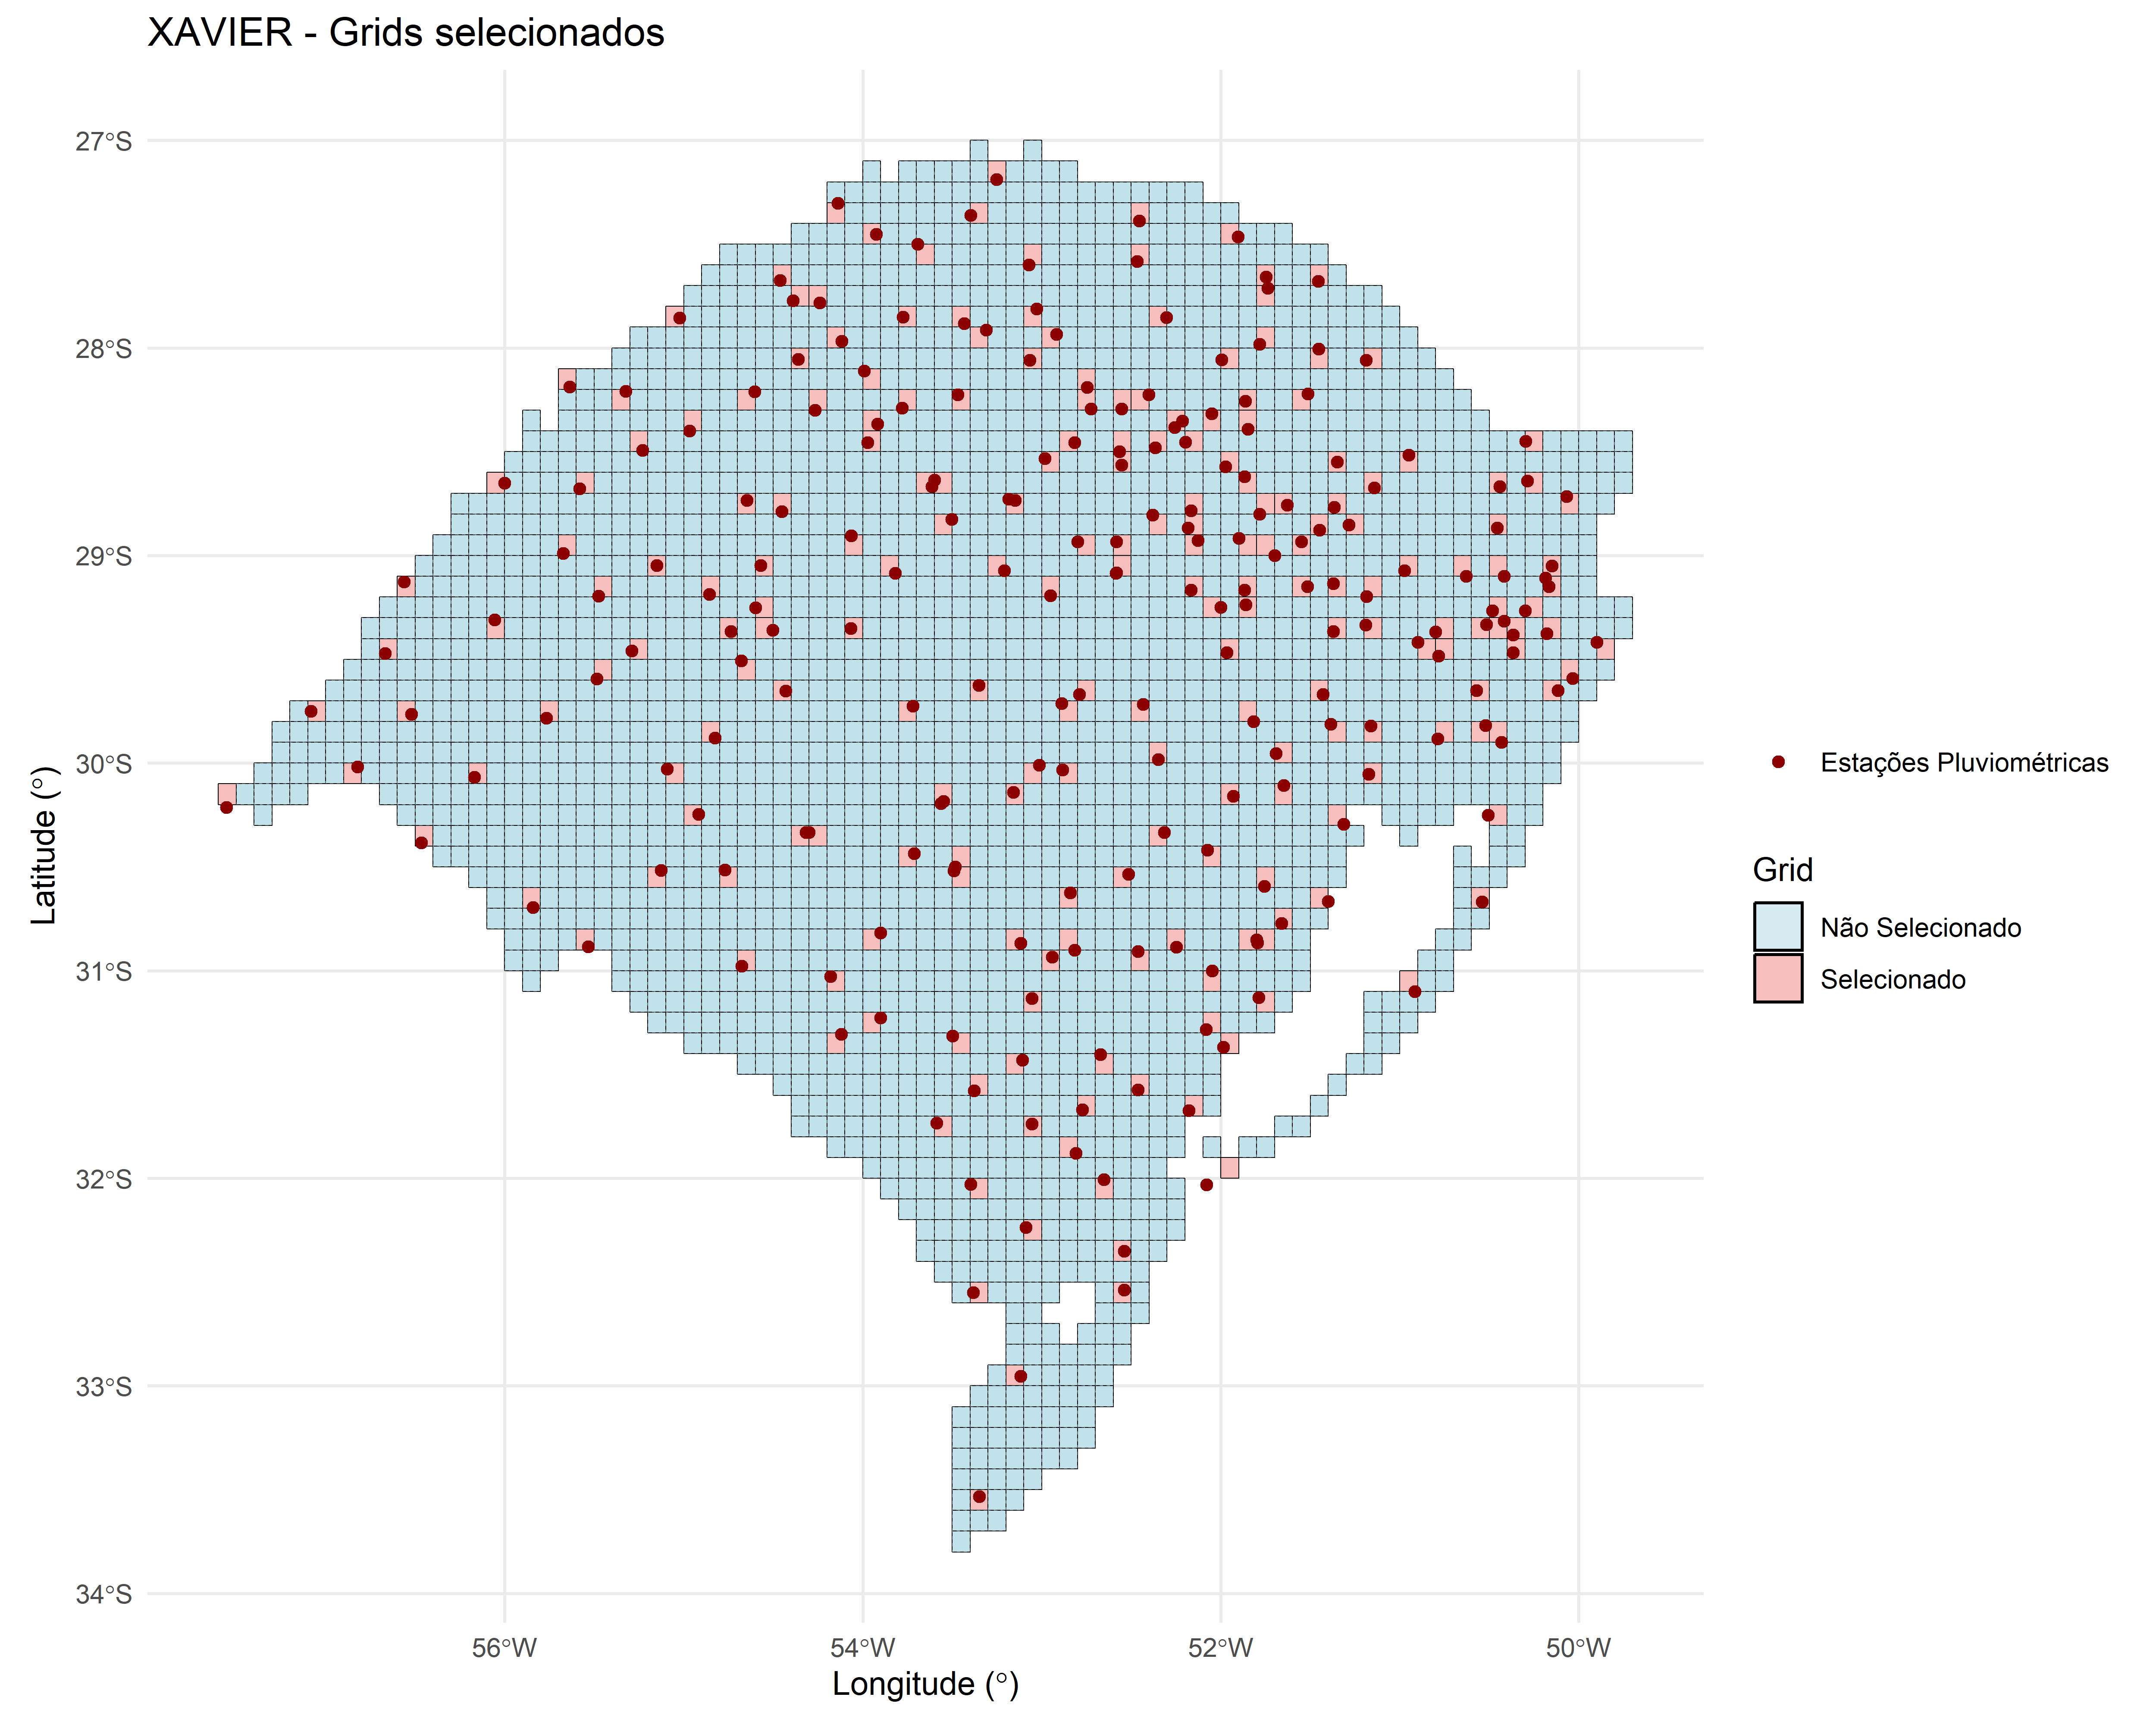
\includegraphics{Figuras/Figura2a.png}

}

\subcaption{\label{fig-Figura2a}Base de dados XAVIER}

\end{minipage}%
\newline
\begin{minipage}{\linewidth}

\centering{

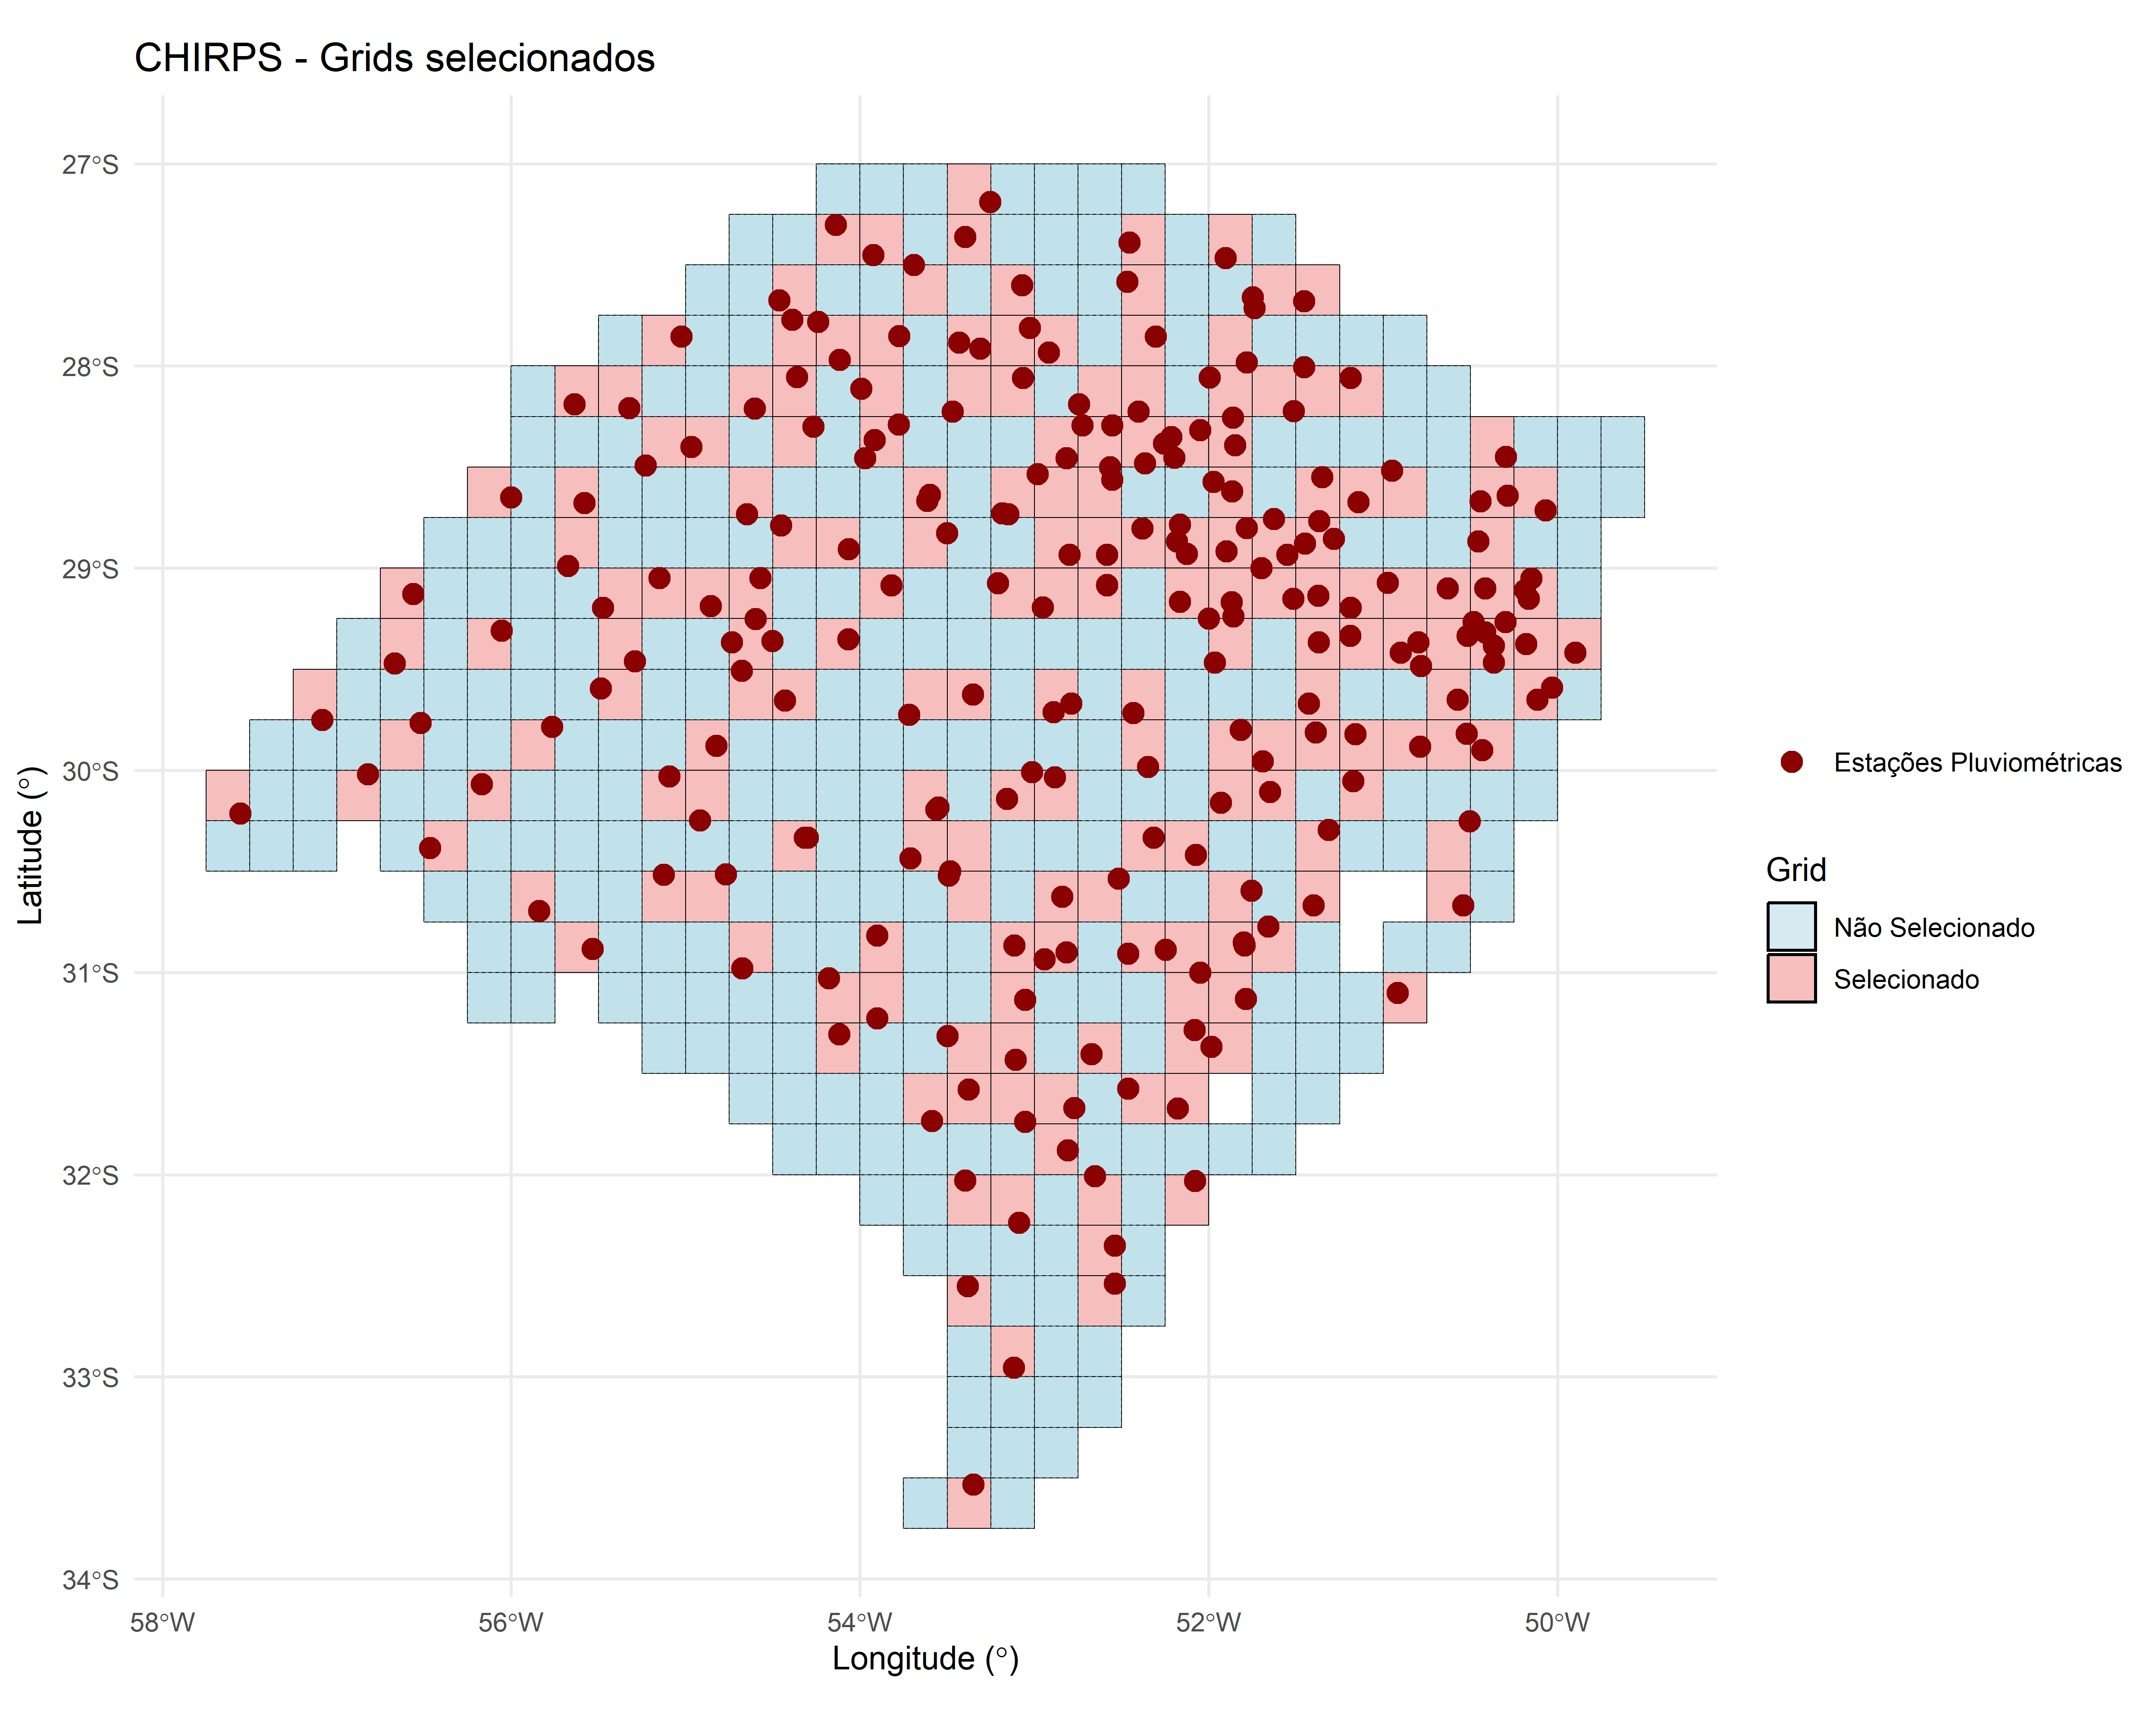
\includegraphics{Figuras/Figura2b.png}

}

\subcaption{\label{fig-Figura2b}Base de dados CHIRPS}

\end{minipage}%

\caption{\label{fig-Figura2}Visualização das celulas de grid
selecionadas para a base XAVIER (a) e CHIRPS (b).Círculos em vermelho
são estações pluviométricas, as células vermelhas indicam os elementos
de grid selecionados para representar as estações e em azul os elementos
de grid que não foram selecionados.}

\end{figure}%

As Figuras 3 a 7 apresentam os resultados para as chuvas com duração de
24 horas para os tempos de retorno de 2, 5, 25, 100 e 500 anos,
respectivamente. Para cada figura as alíneas (a), (b) e (c) mostram os
resultados para a base HIDRO, XAVIER e CHIRPS, respectivamente. A cor e
o tamanho das bolhas referem-se à magnitude das intensidades, sendo as
bolhas maiores e mais avermelhadas representativas de chuvas mais
intensas e as bolhas menores e mais azuladas, menos intensas. A base de
dados HIDRO, sempre representada pela imagem referenciada pela letra
(a), consiste no referencial considerado para comparação com as demais
bases.

Dessa forma, espera-se que os padrões de tamanho e coloração das bolhas
para as bases XAVIER, representada pelas imagens de letra (b) e CHIRPS,
representada pelas imagens de letra (c), possam reproduzir o padrão dos
dados obtidos a partir da base HIDRO. A partir da análise dos
resultados, observa-se que para ambas as bases em grade, há um viés em
subestimar os valores de intensidade de chuva, sendo esse viés mais
acentuado para a base CHIRPS. Observa-se que esse viés tende a aumentar
à medida que o tempo de retorno aumenta. Esse fato pode estar associado
com o aumento esperado de incertezas para chuvas com tempo de
recorrência maiores.

Os resultados dessa comparação sugerem ainda que a base XAVIER parece
representar melhor o padrão espacial das chuvas e suas intensidades em
relação à base HIDRO, quando comparado com a base CHIRPS. Alguns
aspectos podem estar associados à esta melhor correspondência. Um deles
refere-se ao fato de a base XAVIER possuir uma menor resolução espacial,
quando comparada com a base CHIRPS. Outro fator pode estar relacionado à
base de dados e metodologia utilizadas para composição da grade XAVIER,
que deve ter uma melhor representatividade da área de interesse, já que
esta base foi construída com o propósito de representar os padrões
espaciais de chuva da região da América do Sul, enquanto a base CHIRPS
tem um propósito de representação dos padrões espaciais de chuva
praticamente de todo o planeta.

\begin{figure}

\begin{minipage}{\linewidth}

\centering{

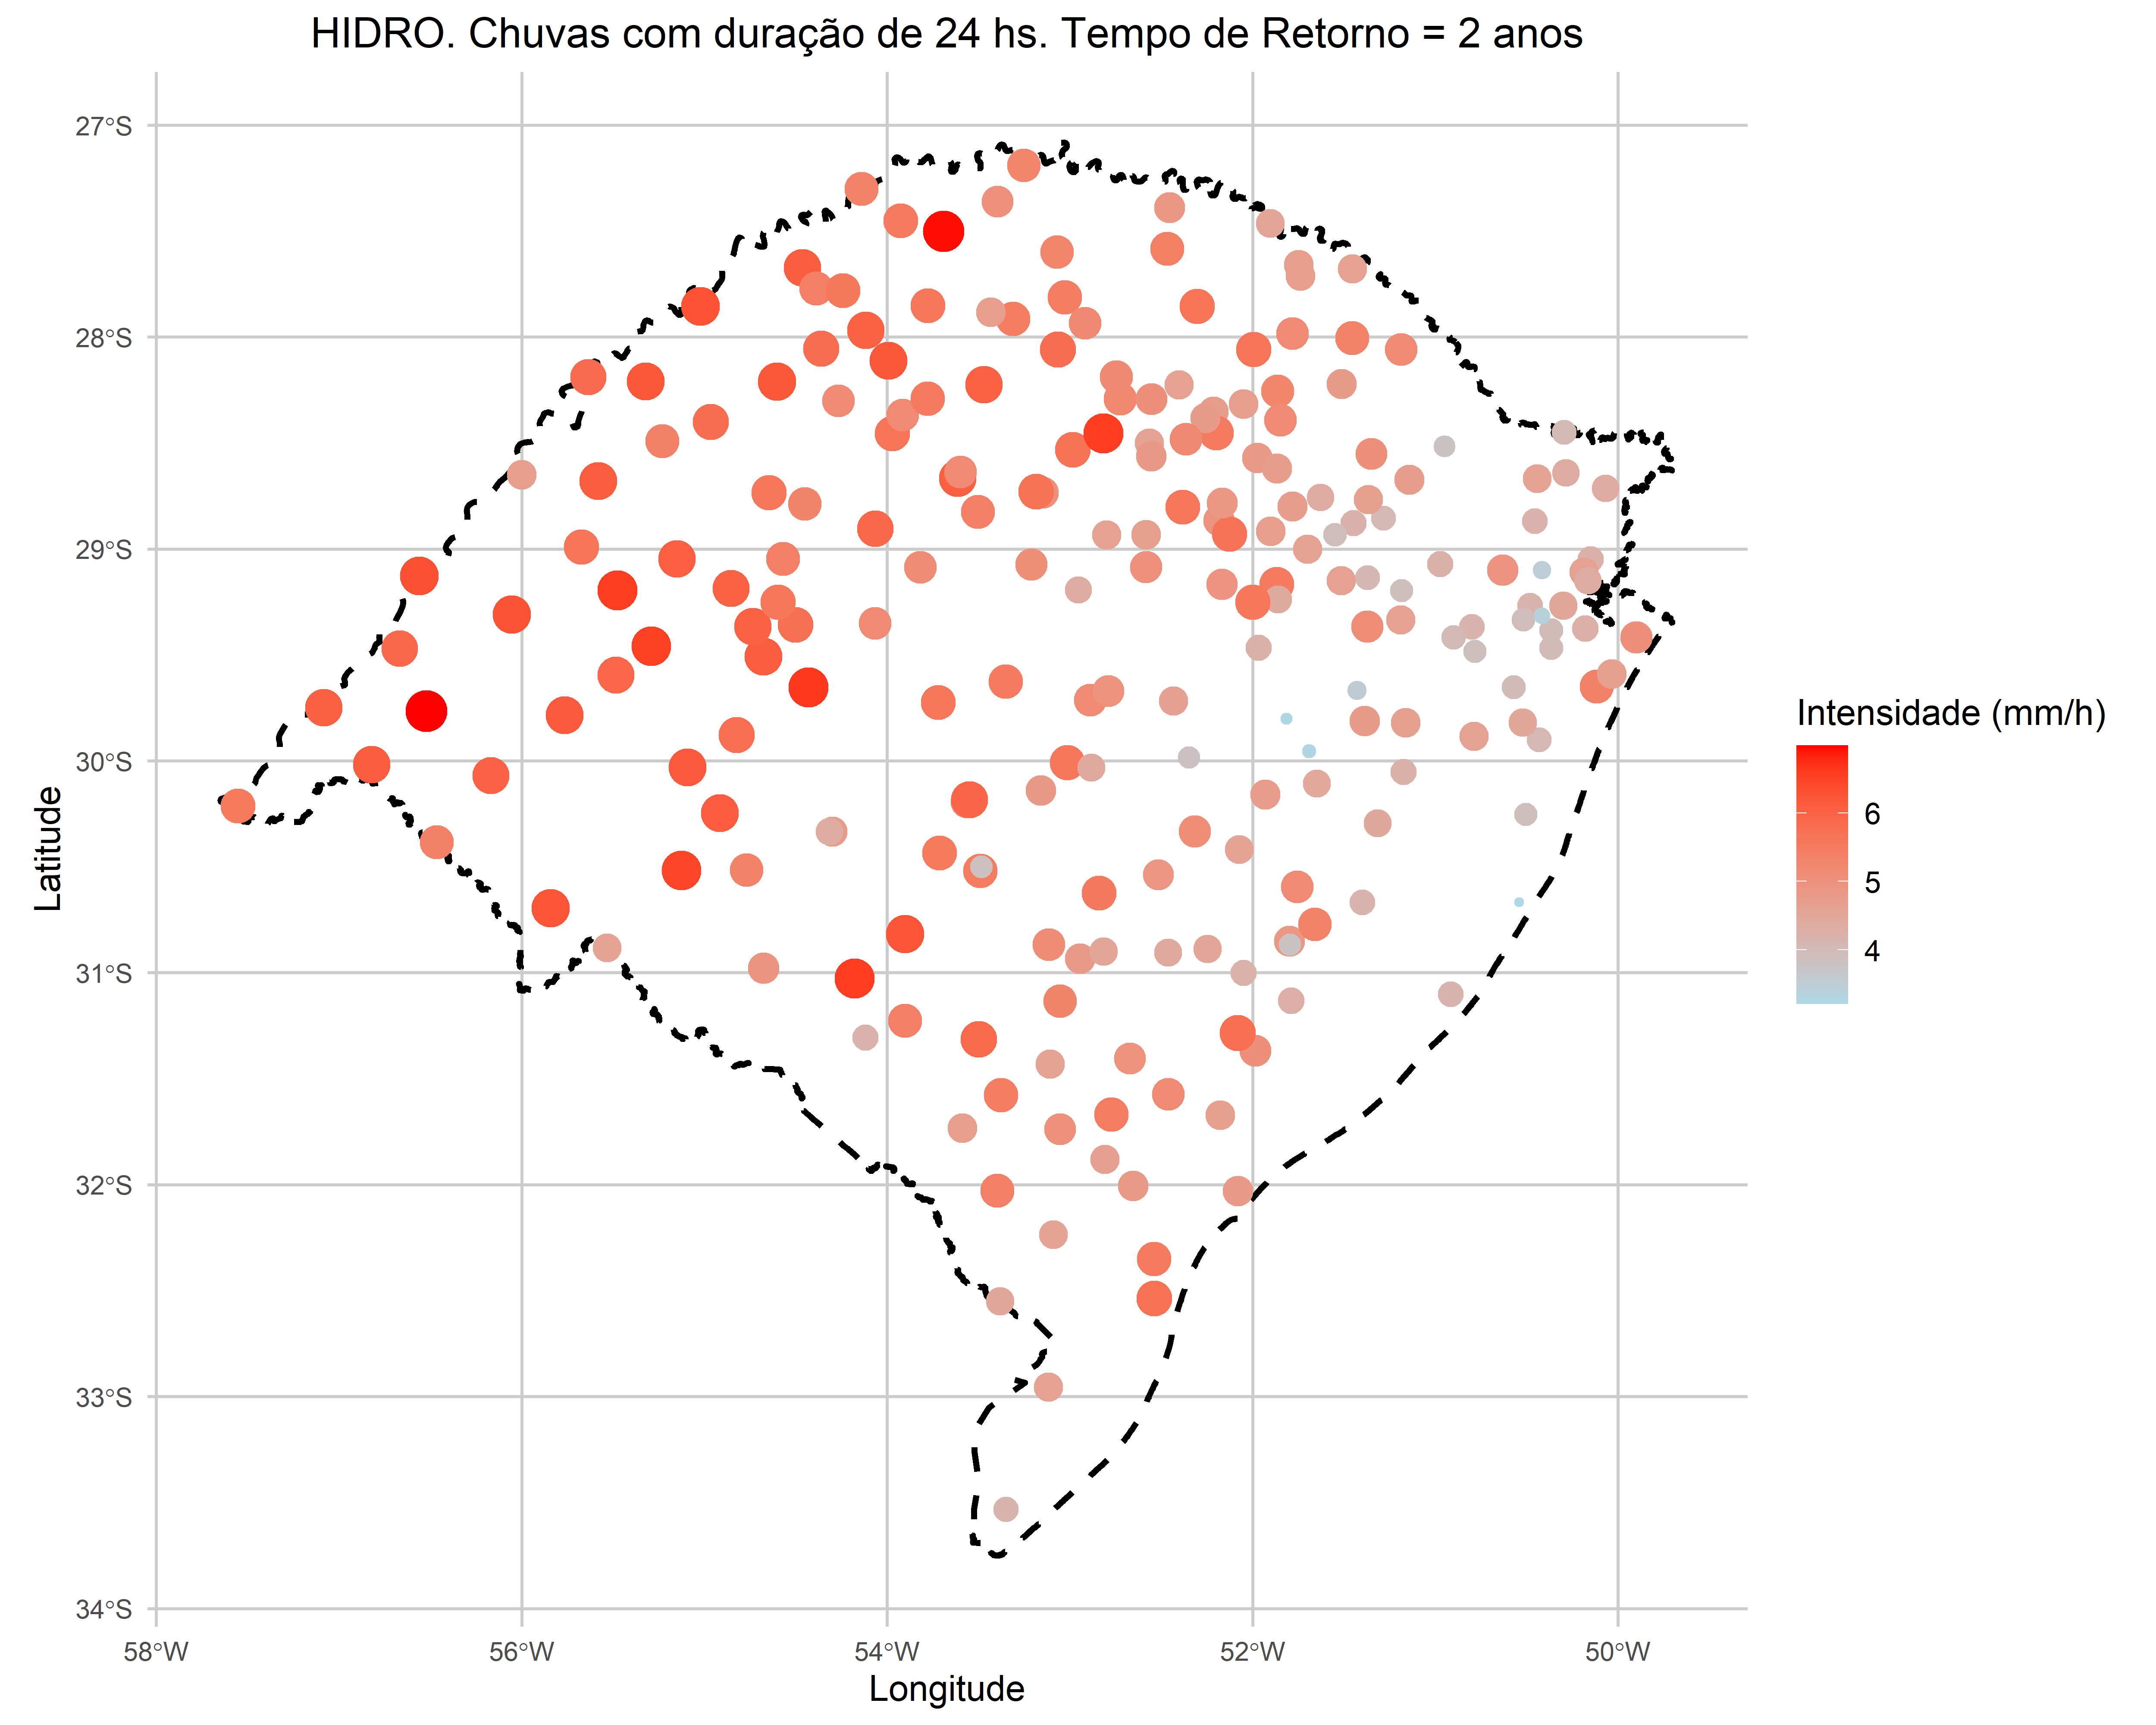
\includegraphics{Figuras/Figura3a.png}

}

\subcaption{\label{fig-Figura3a}Base de dados HIDRO}

\end{minipage}%
\newline
\begin{minipage}{\linewidth}

\centering{

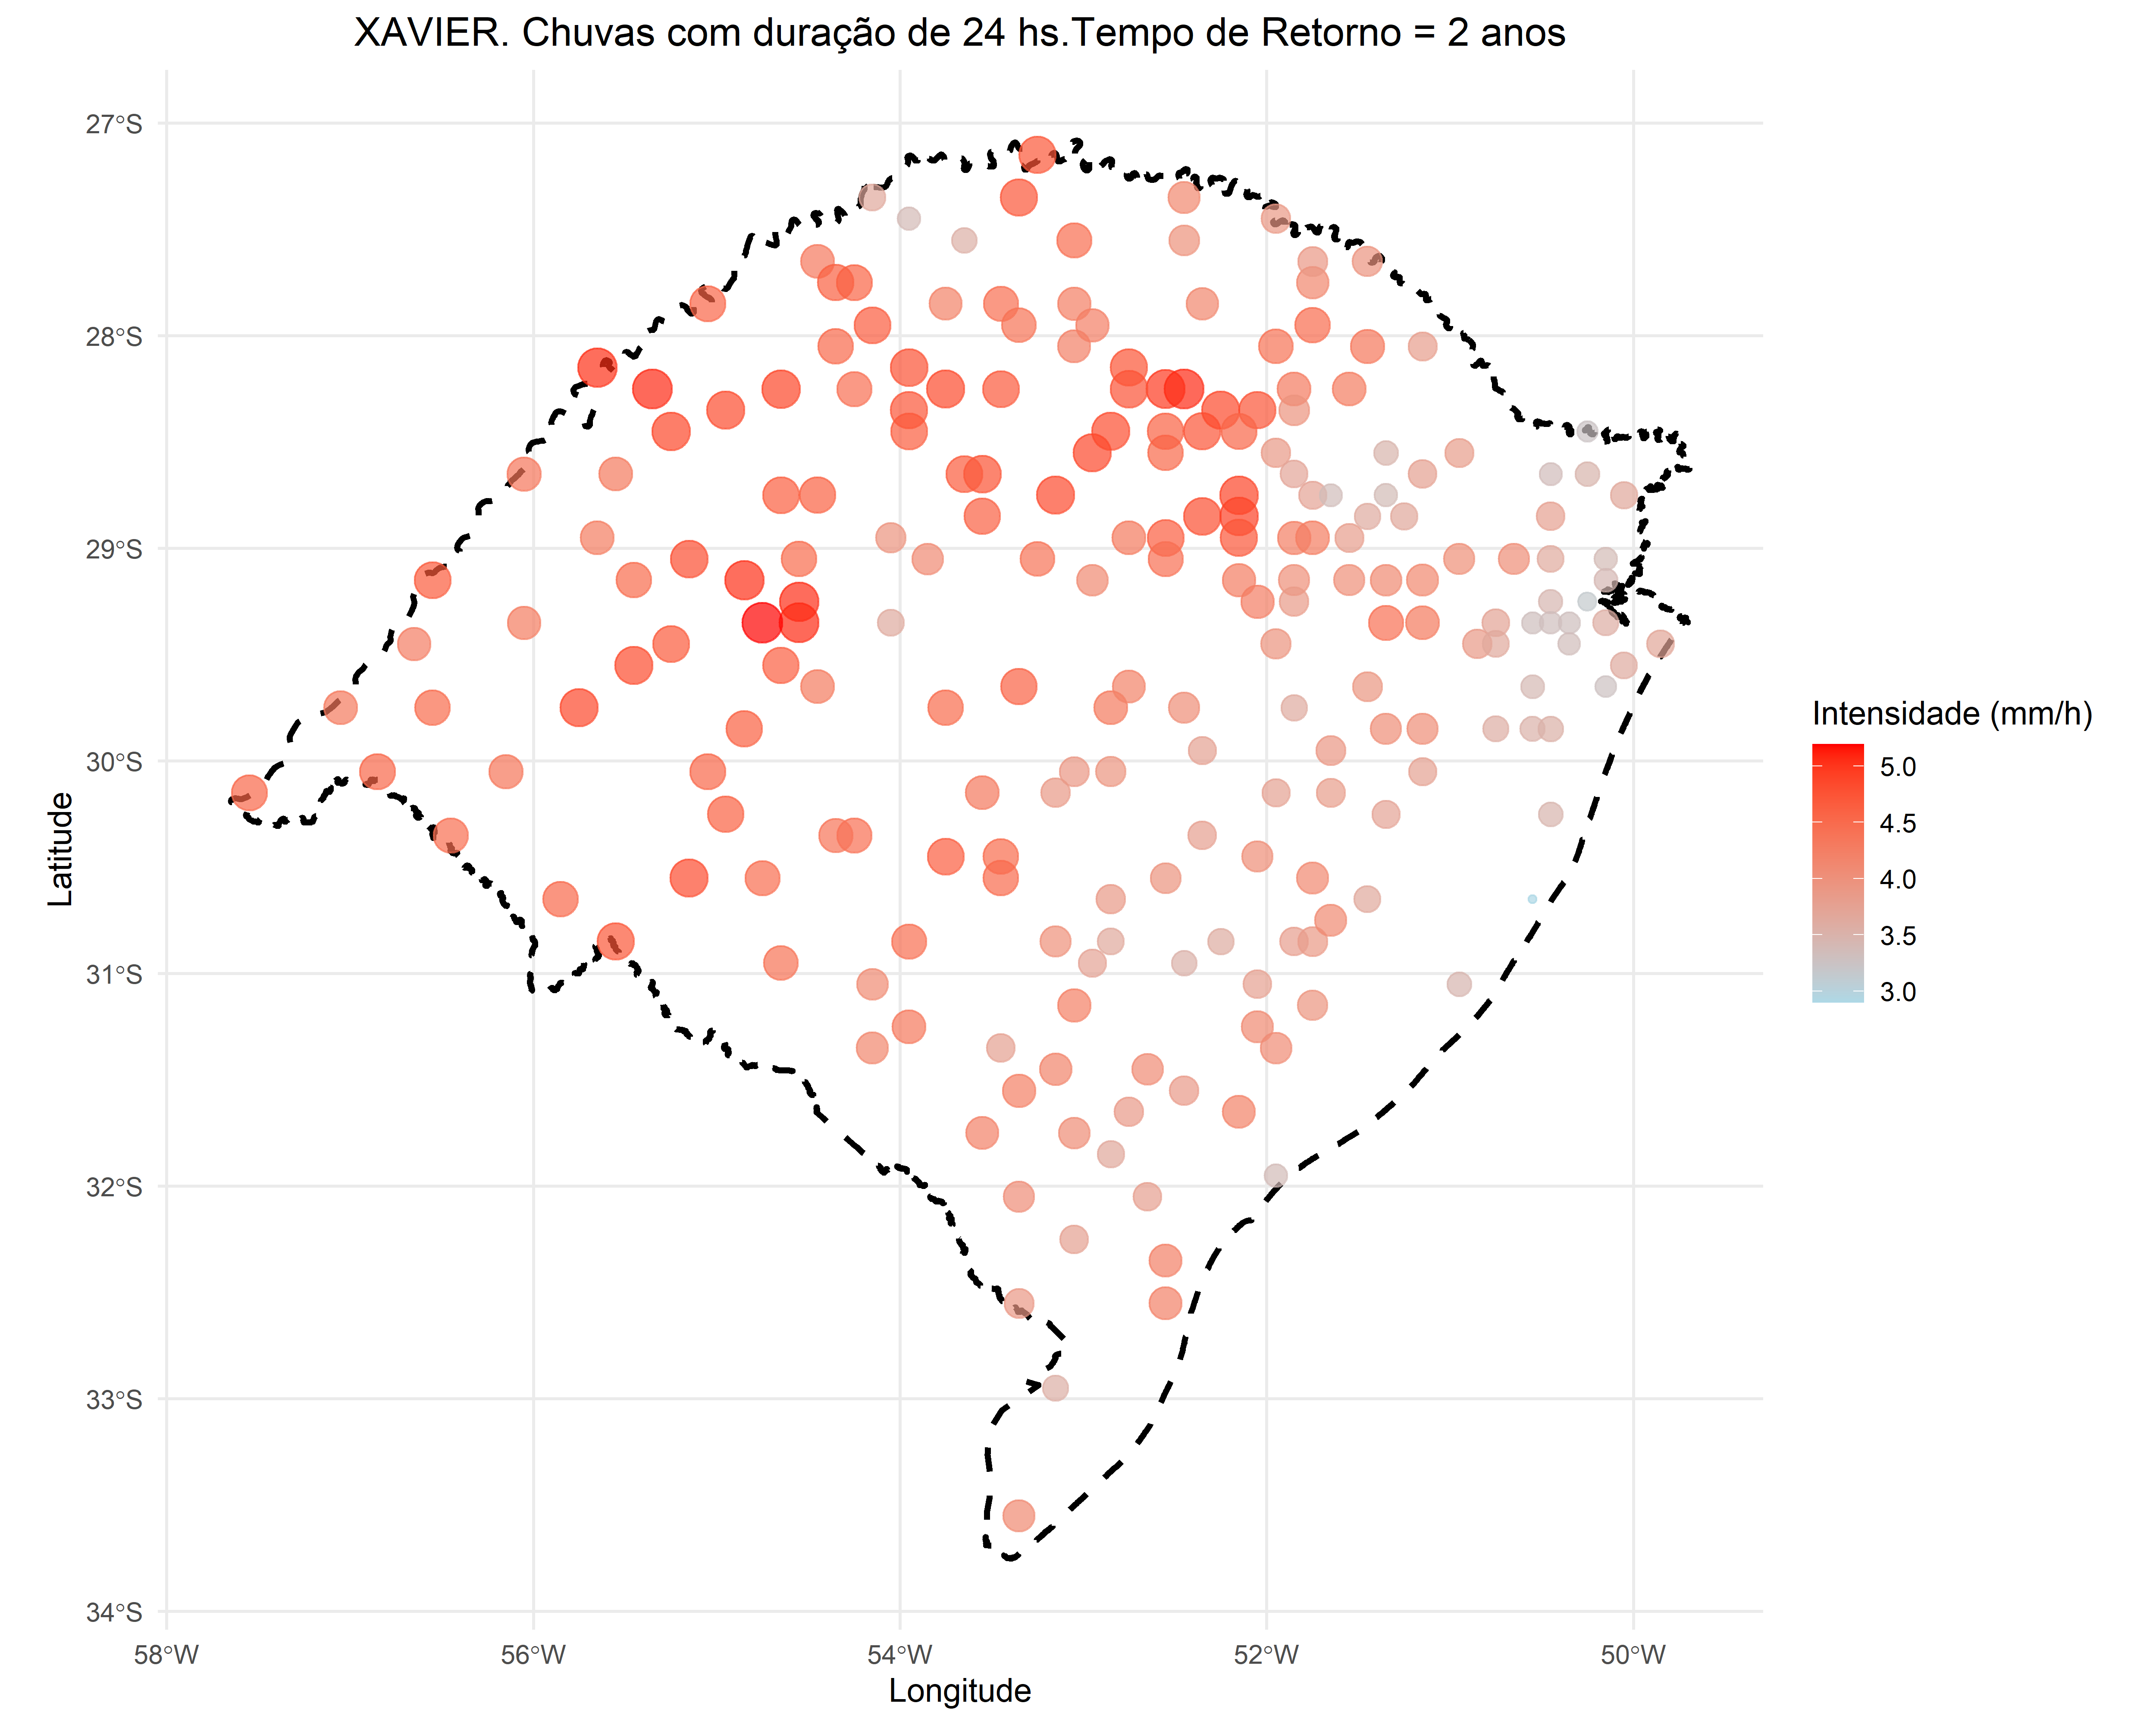
\includegraphics{Figuras/Figura3b.png}

}

\subcaption{\label{fig-Figura3b}Base de dados XAVIER}

\end{minipage}%
\newline
\begin{minipage}{\linewidth}

\centering{

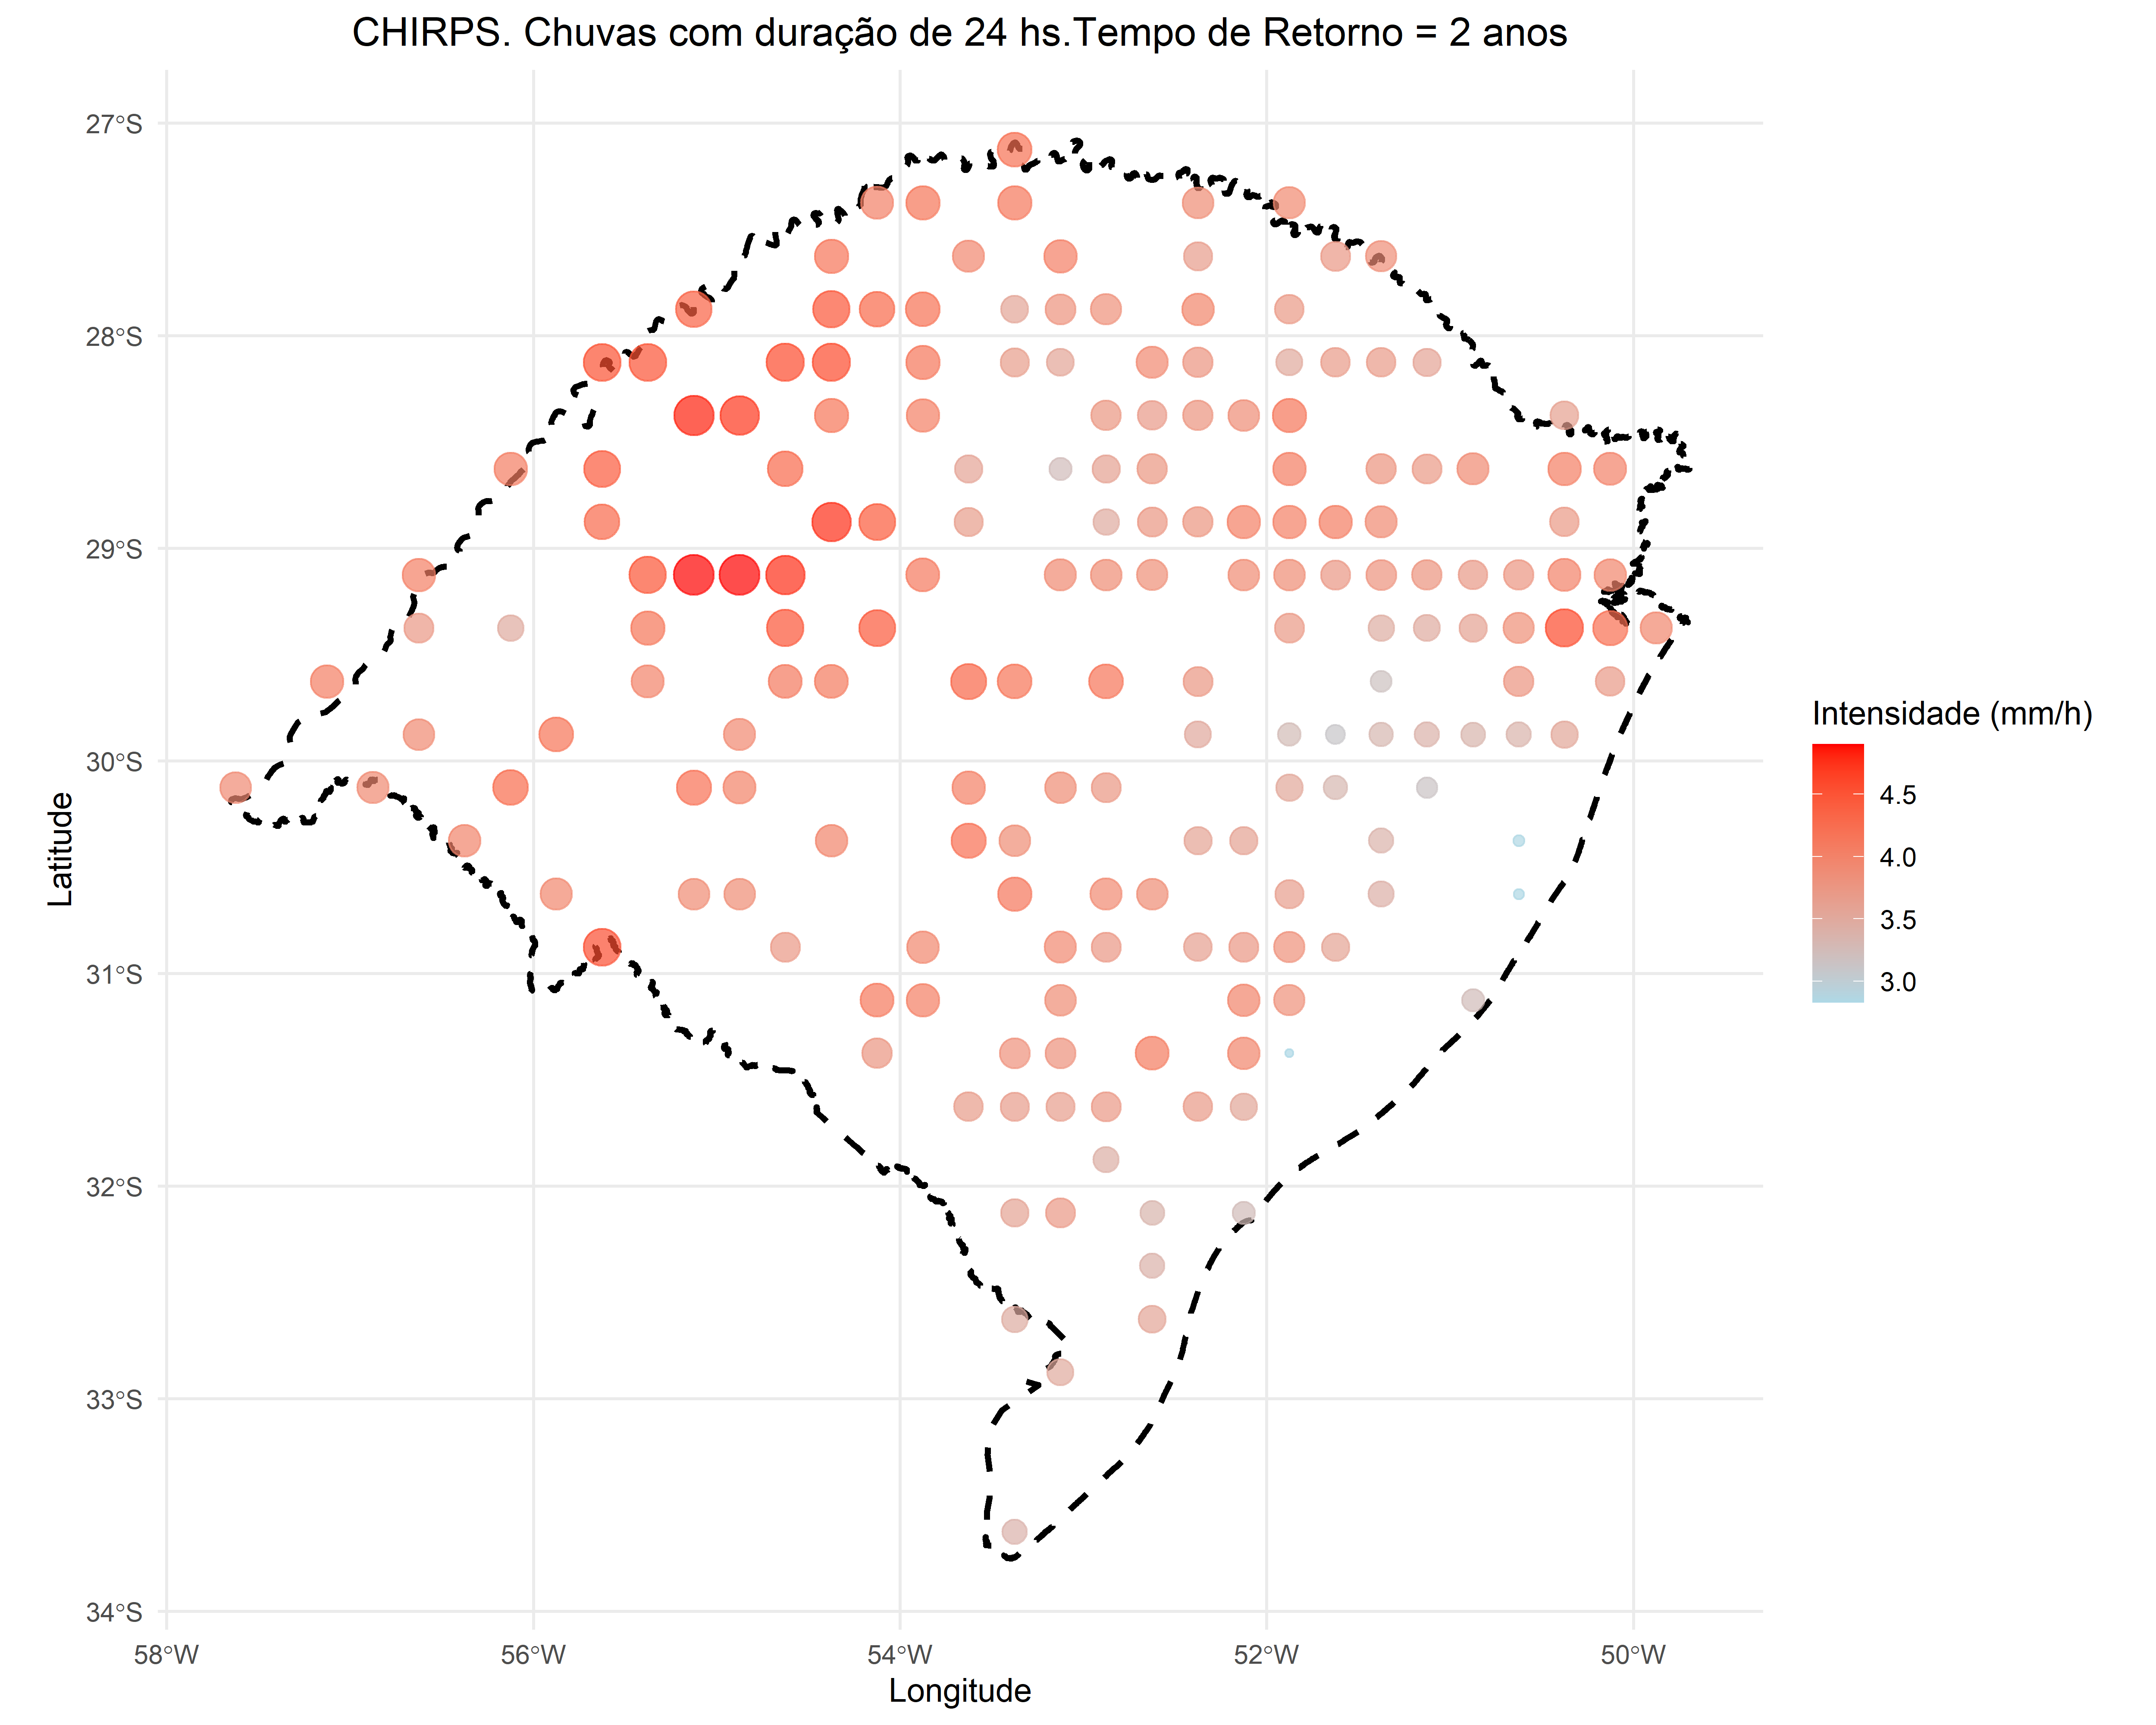
\includegraphics{Figuras/Figura3c.png}

}

\subcaption{\label{fig-Figura3c}Base de dados CHIRPS}

\end{minipage}%

\caption{\label{fig-Figura3}Magnitude da intensidade da precipitação com
duração de 24 horas para o tempo de retorno de 2 anos considerando a
base de dados HDIRO (a); XAVIER (b) e CHIRPS (c). O tamanho dos circulos
azuis indica a magnitude da intensidade das chuvas.}

\end{figure}%

\begin{figure}

\begin{minipage}{\linewidth}

\centering{

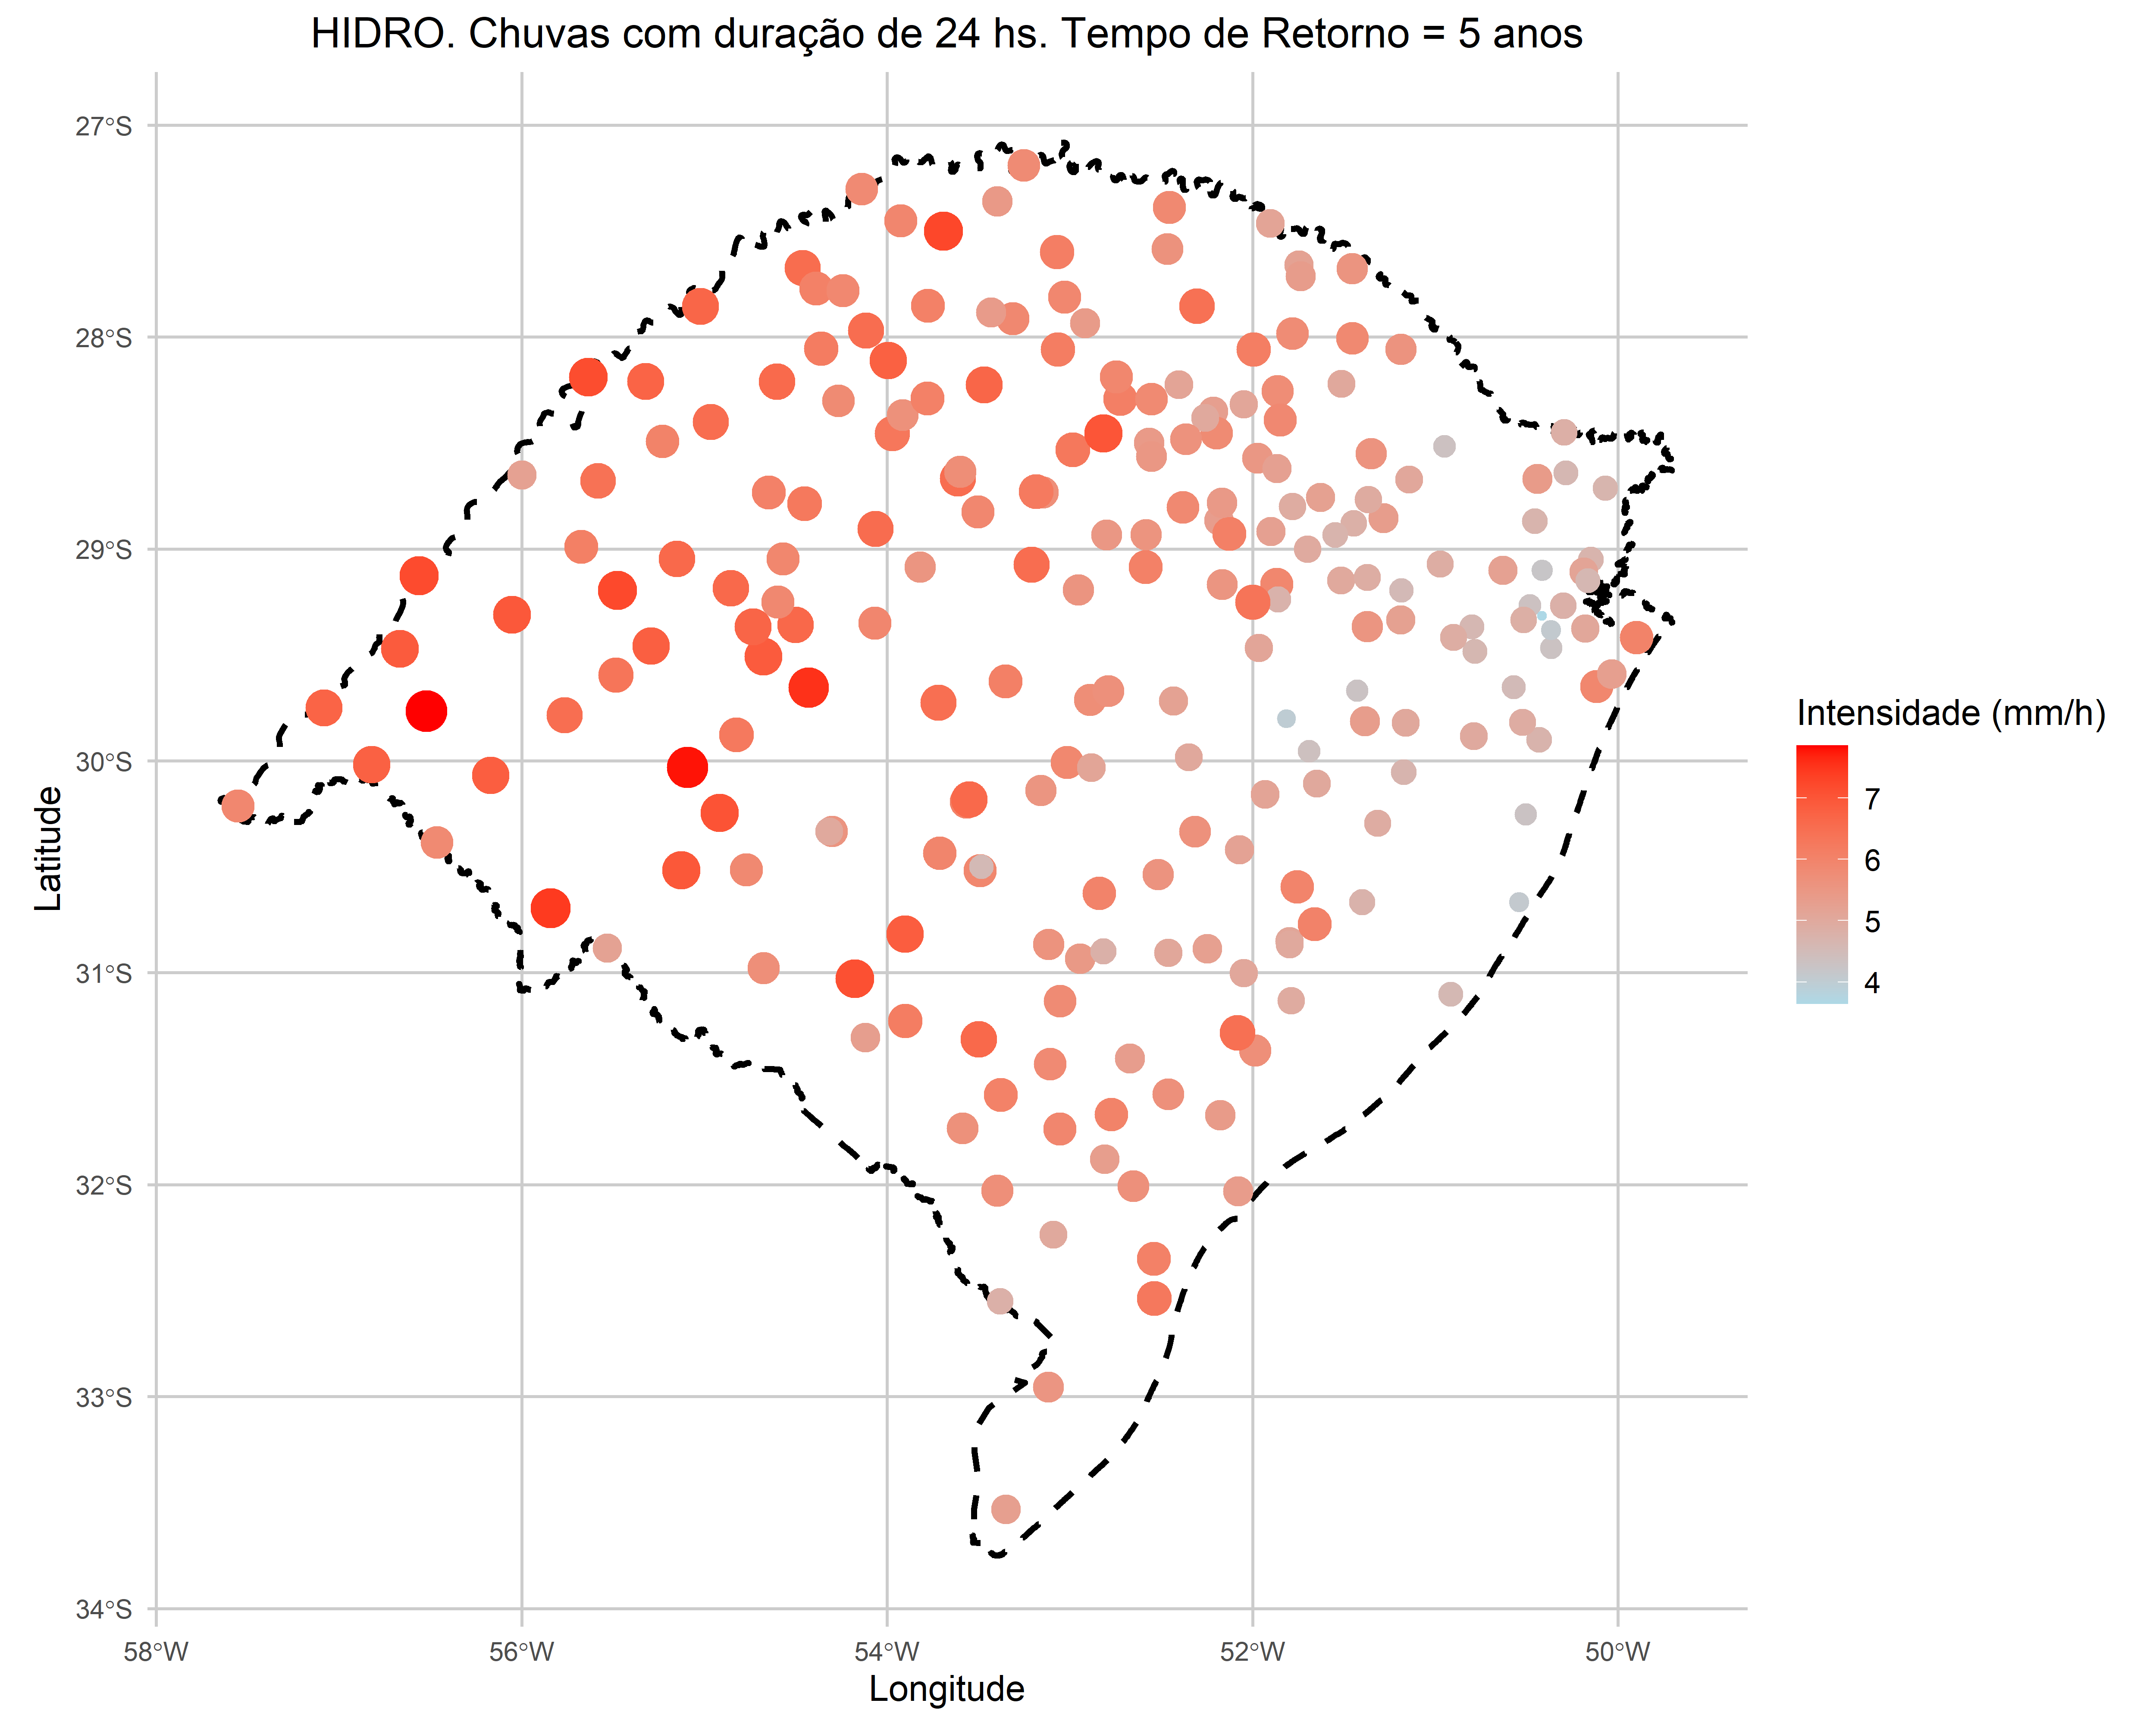
\includegraphics{Figuras/Figura4a.png}

}

\subcaption{\label{fig-Figura4a}Base de dados HIDRO}

\end{minipage}%
\newline
\begin{minipage}{\linewidth}

\centering{

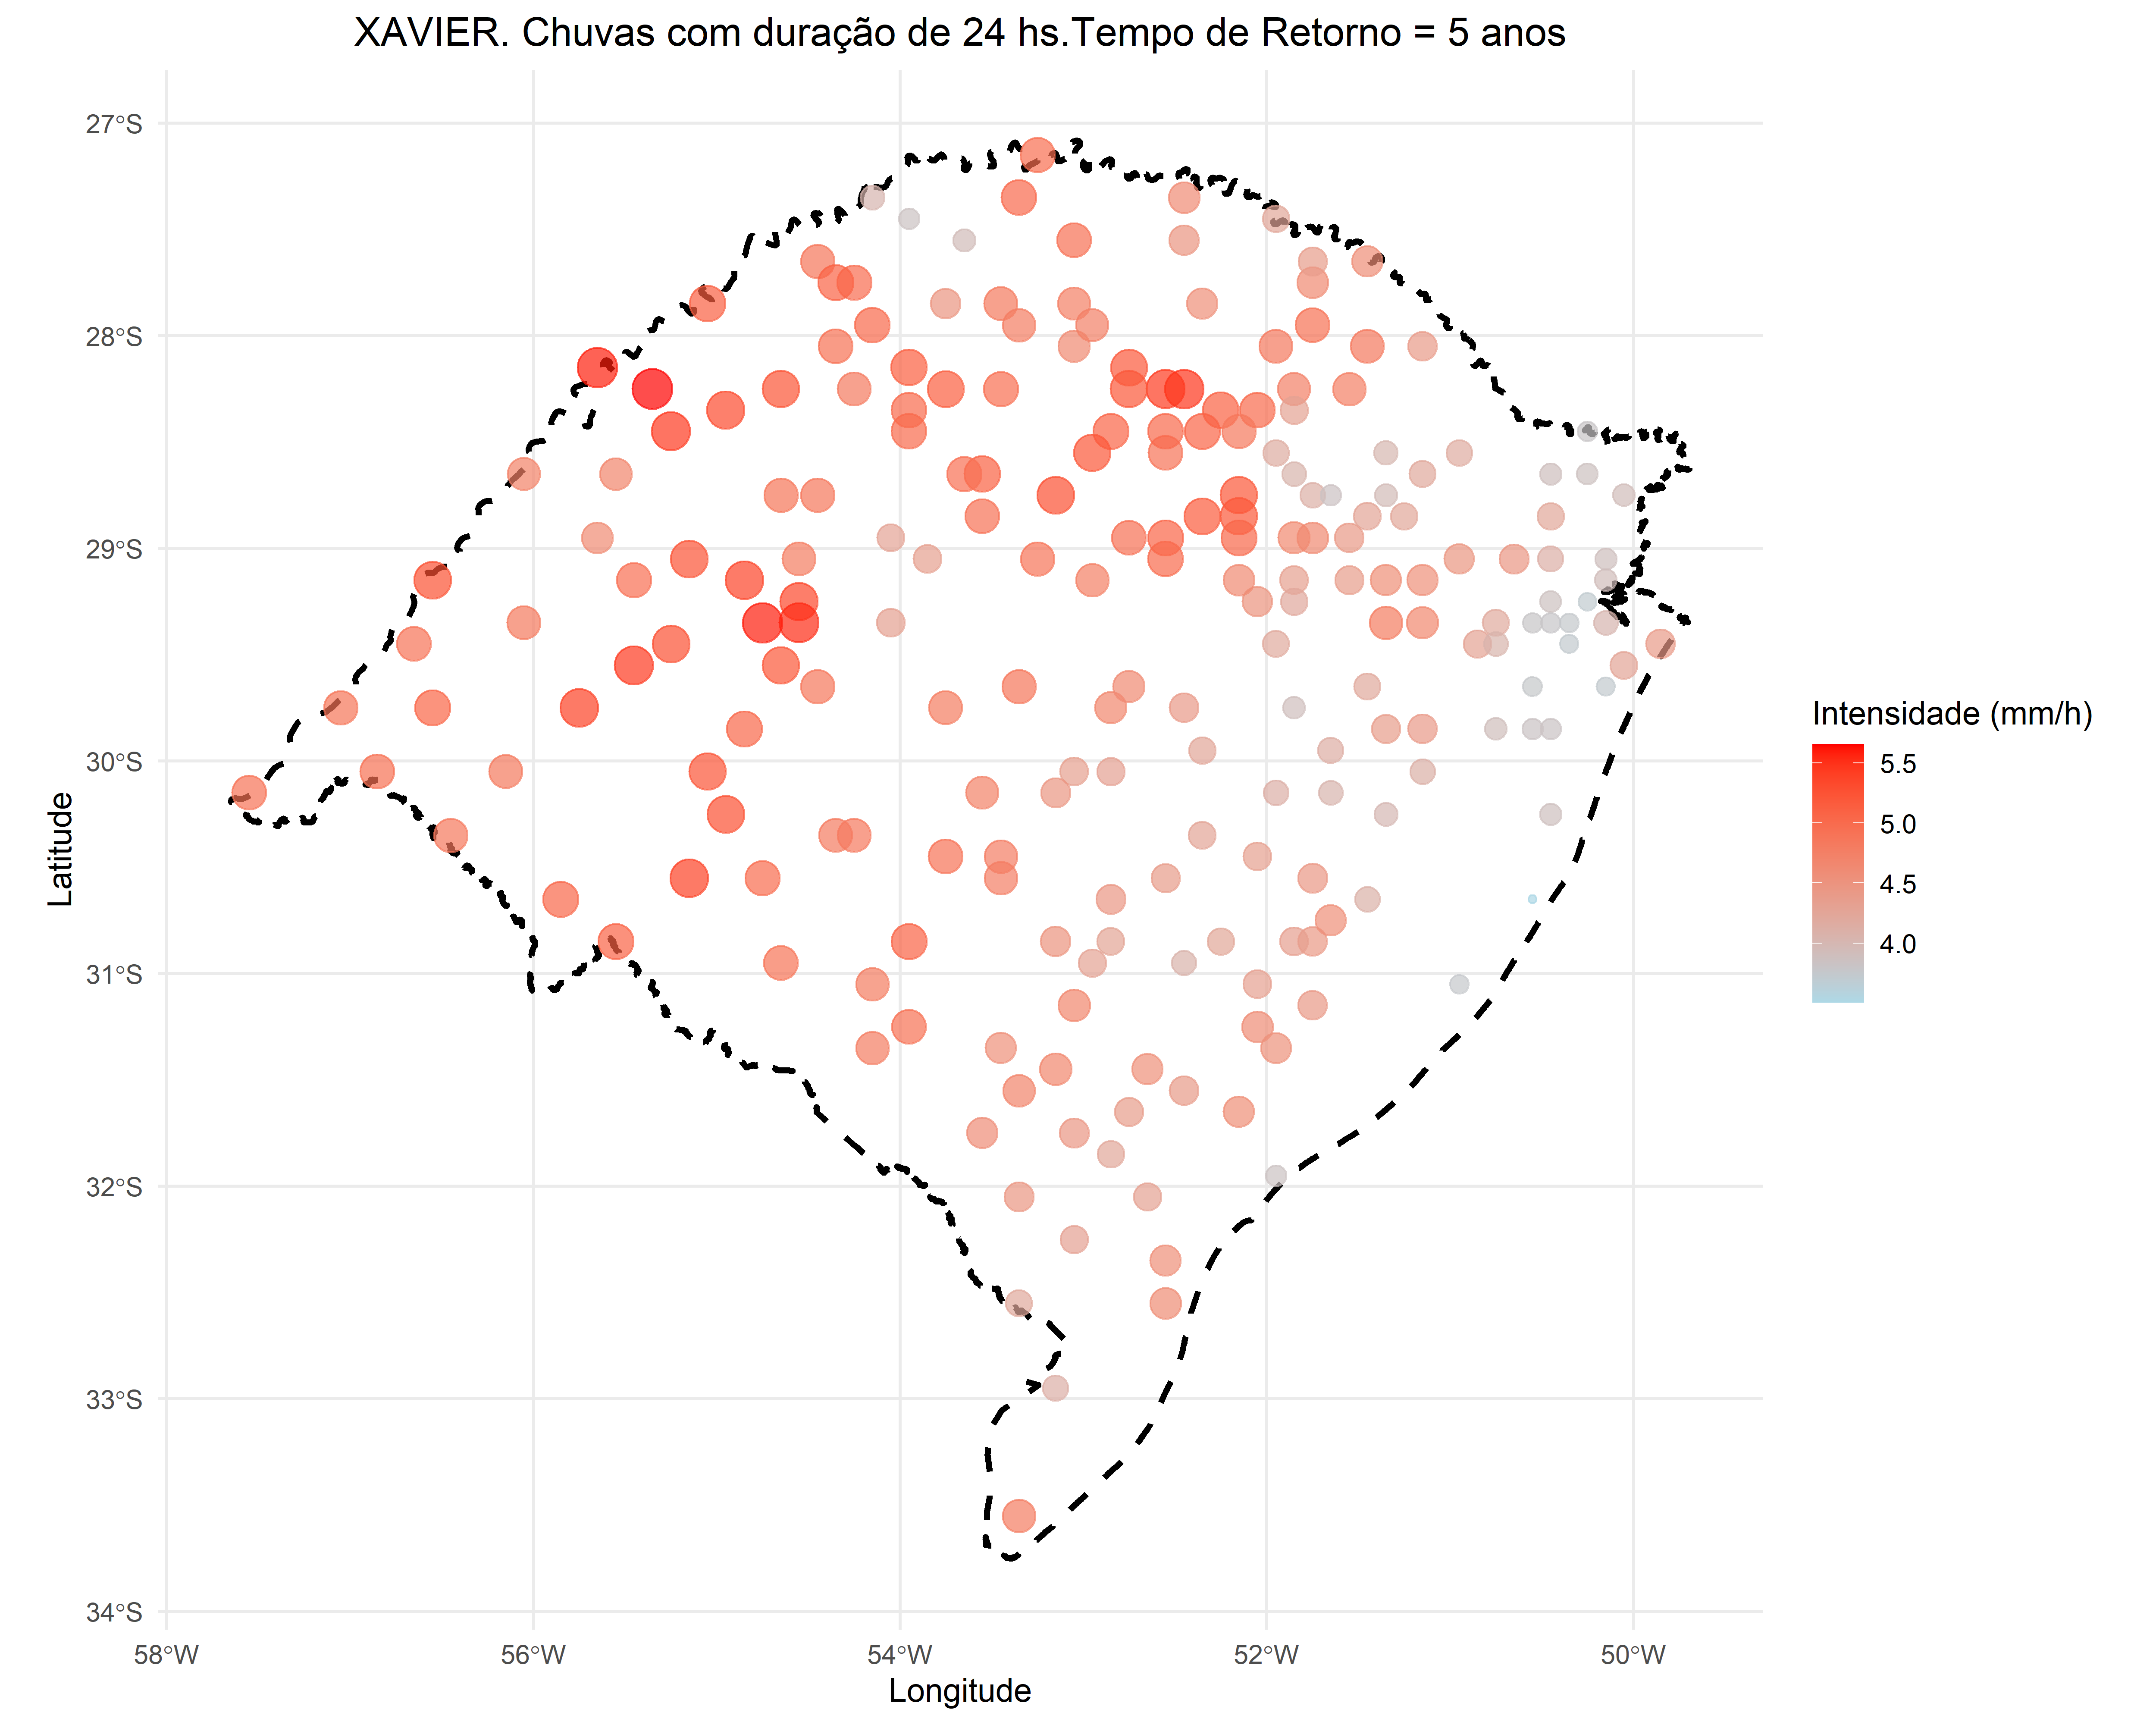
\includegraphics{Figuras/Figura4b.png}

}

\subcaption{\label{fig-Figura4b}Base de dados XAVIER}

\end{minipage}%
\newline
\begin{minipage}{\linewidth}

\centering{

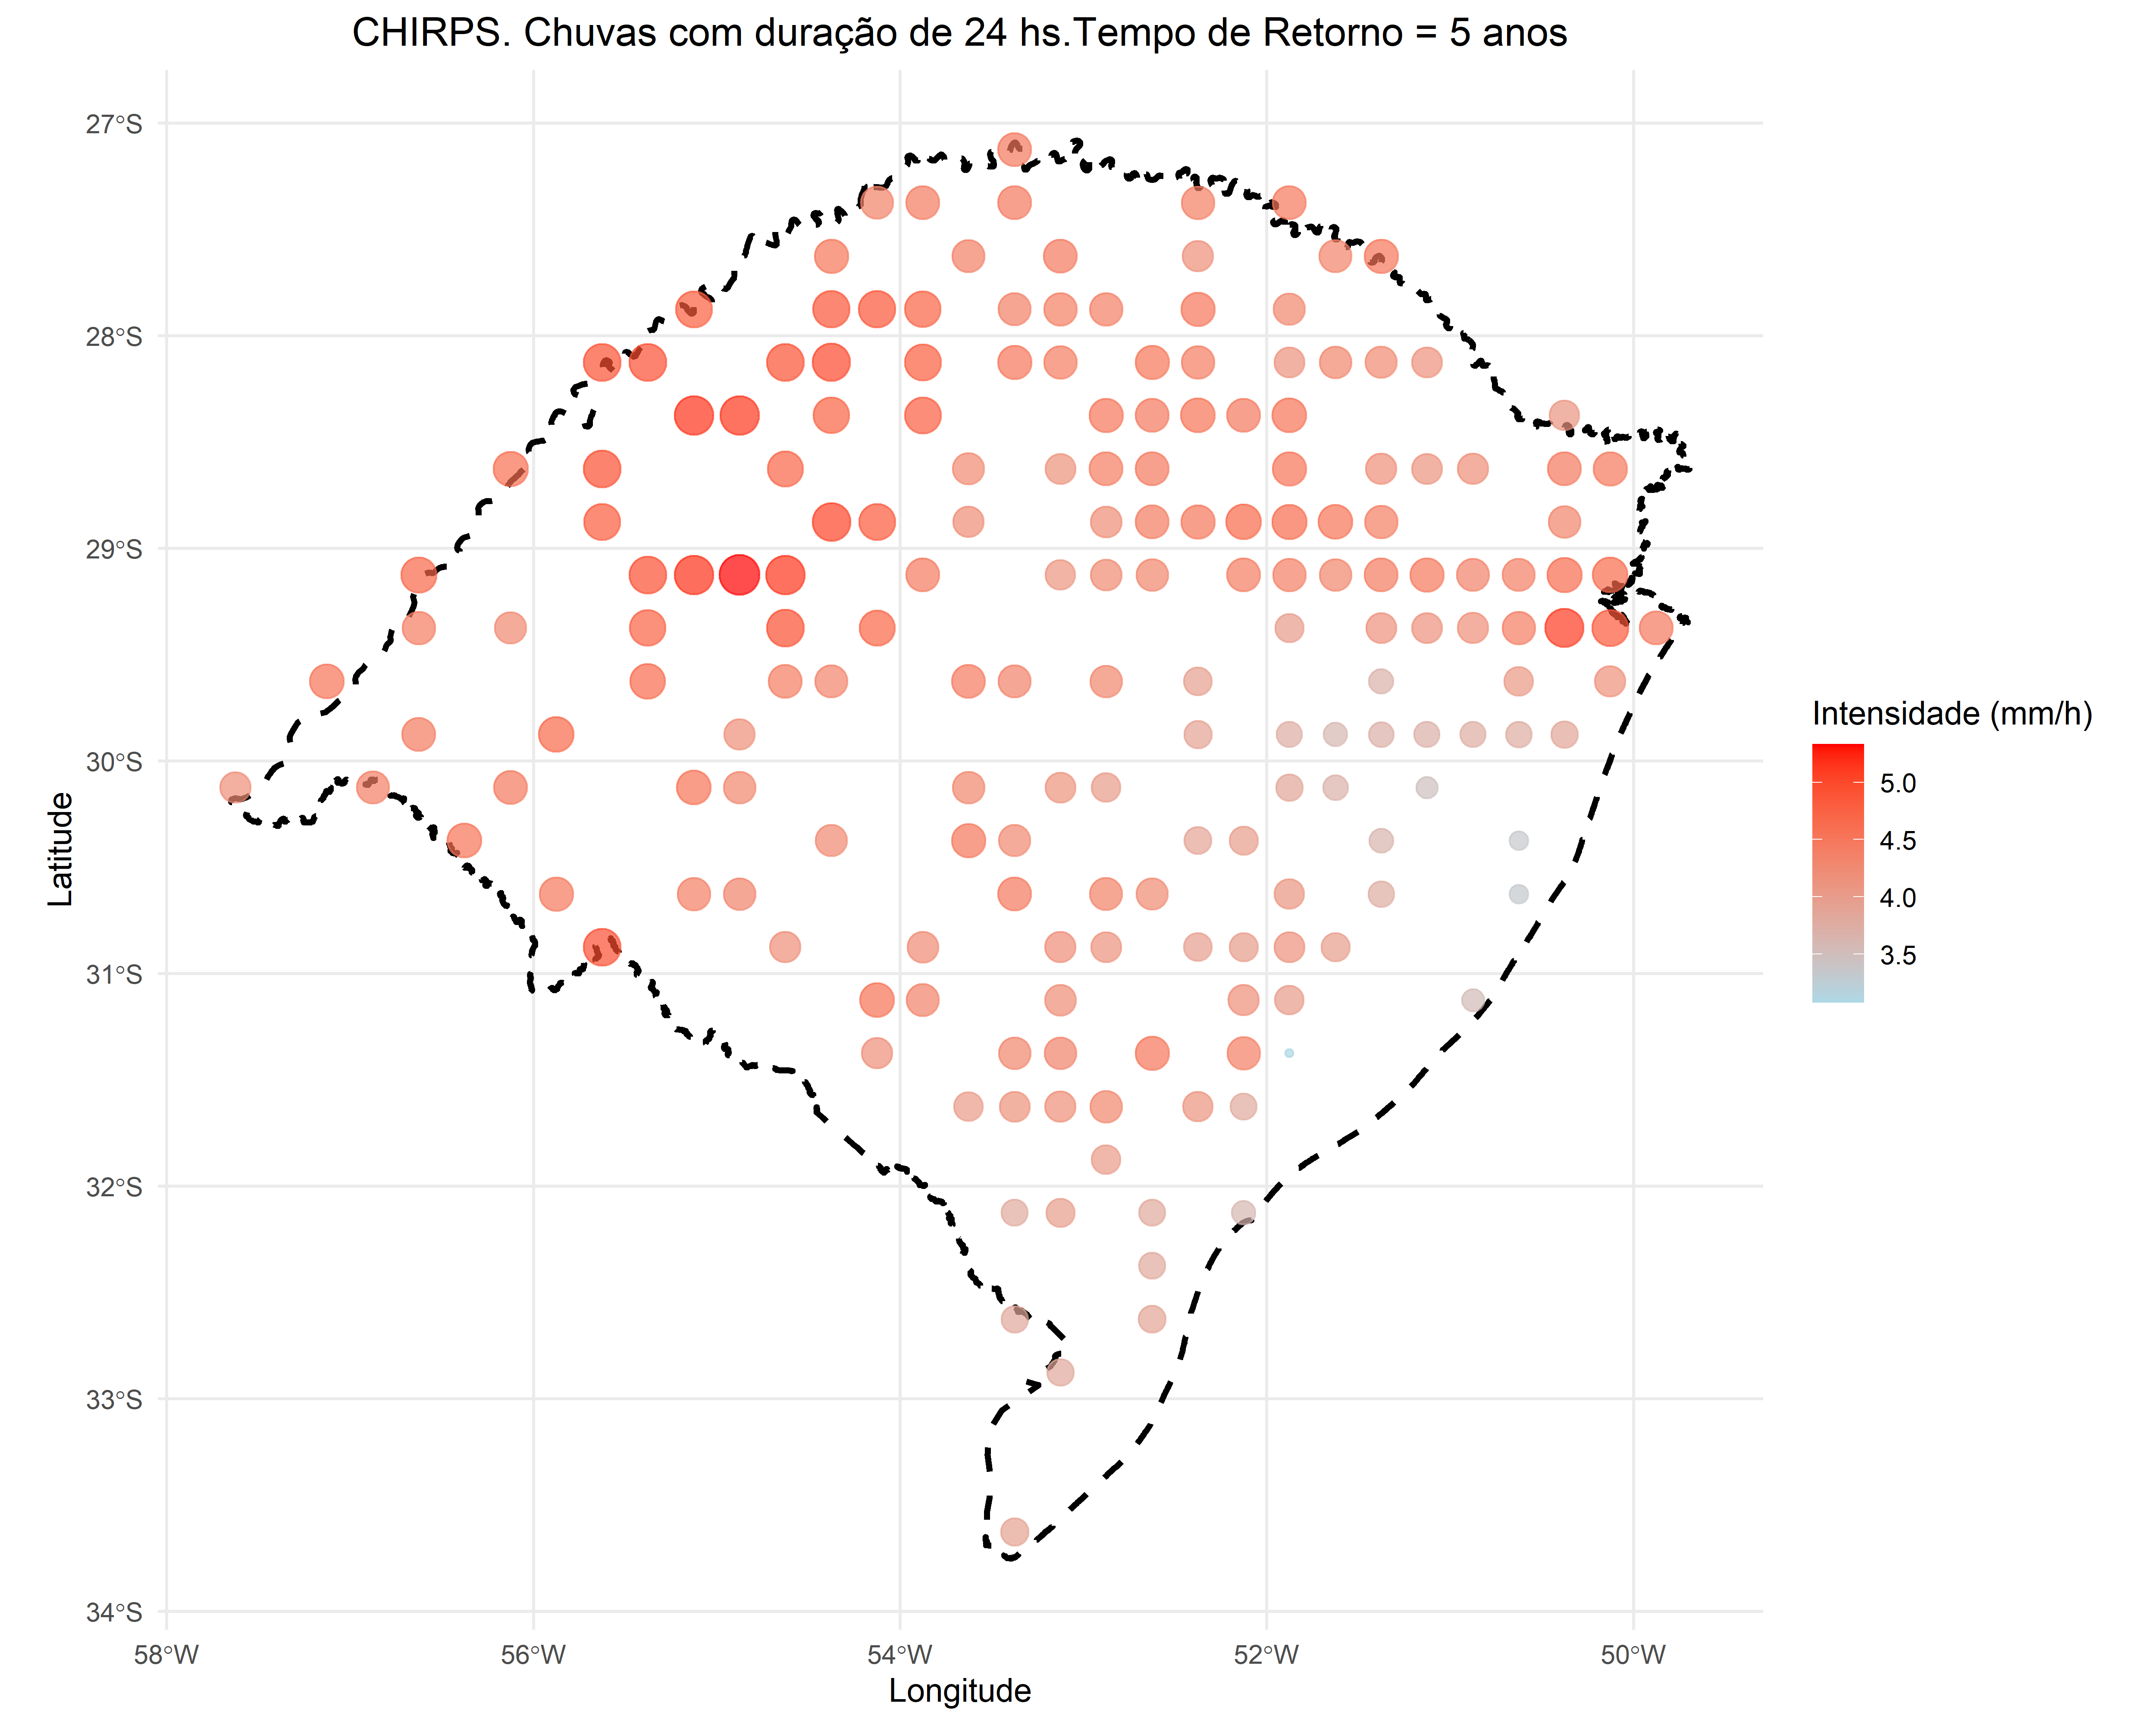
\includegraphics{Figuras/Figura4c.png}

}

\subcaption{\label{fig-Figura4c}Base de dados CHIRPS}

\end{minipage}%

\caption{\label{fig-Figura4}Magnitude da intensidade da precipitação com
duração de 24 horas para o tempo de retorno de 5 anos considerando a
base de dados HDIRO (a); XAVIER (b) e CHIRPS (c). O tamanho dos circulos
azuis indica a magnitude da intensidade das chuvas.}

\end{figure}%

\begin{figure}

\begin{minipage}{\linewidth}

\centering{

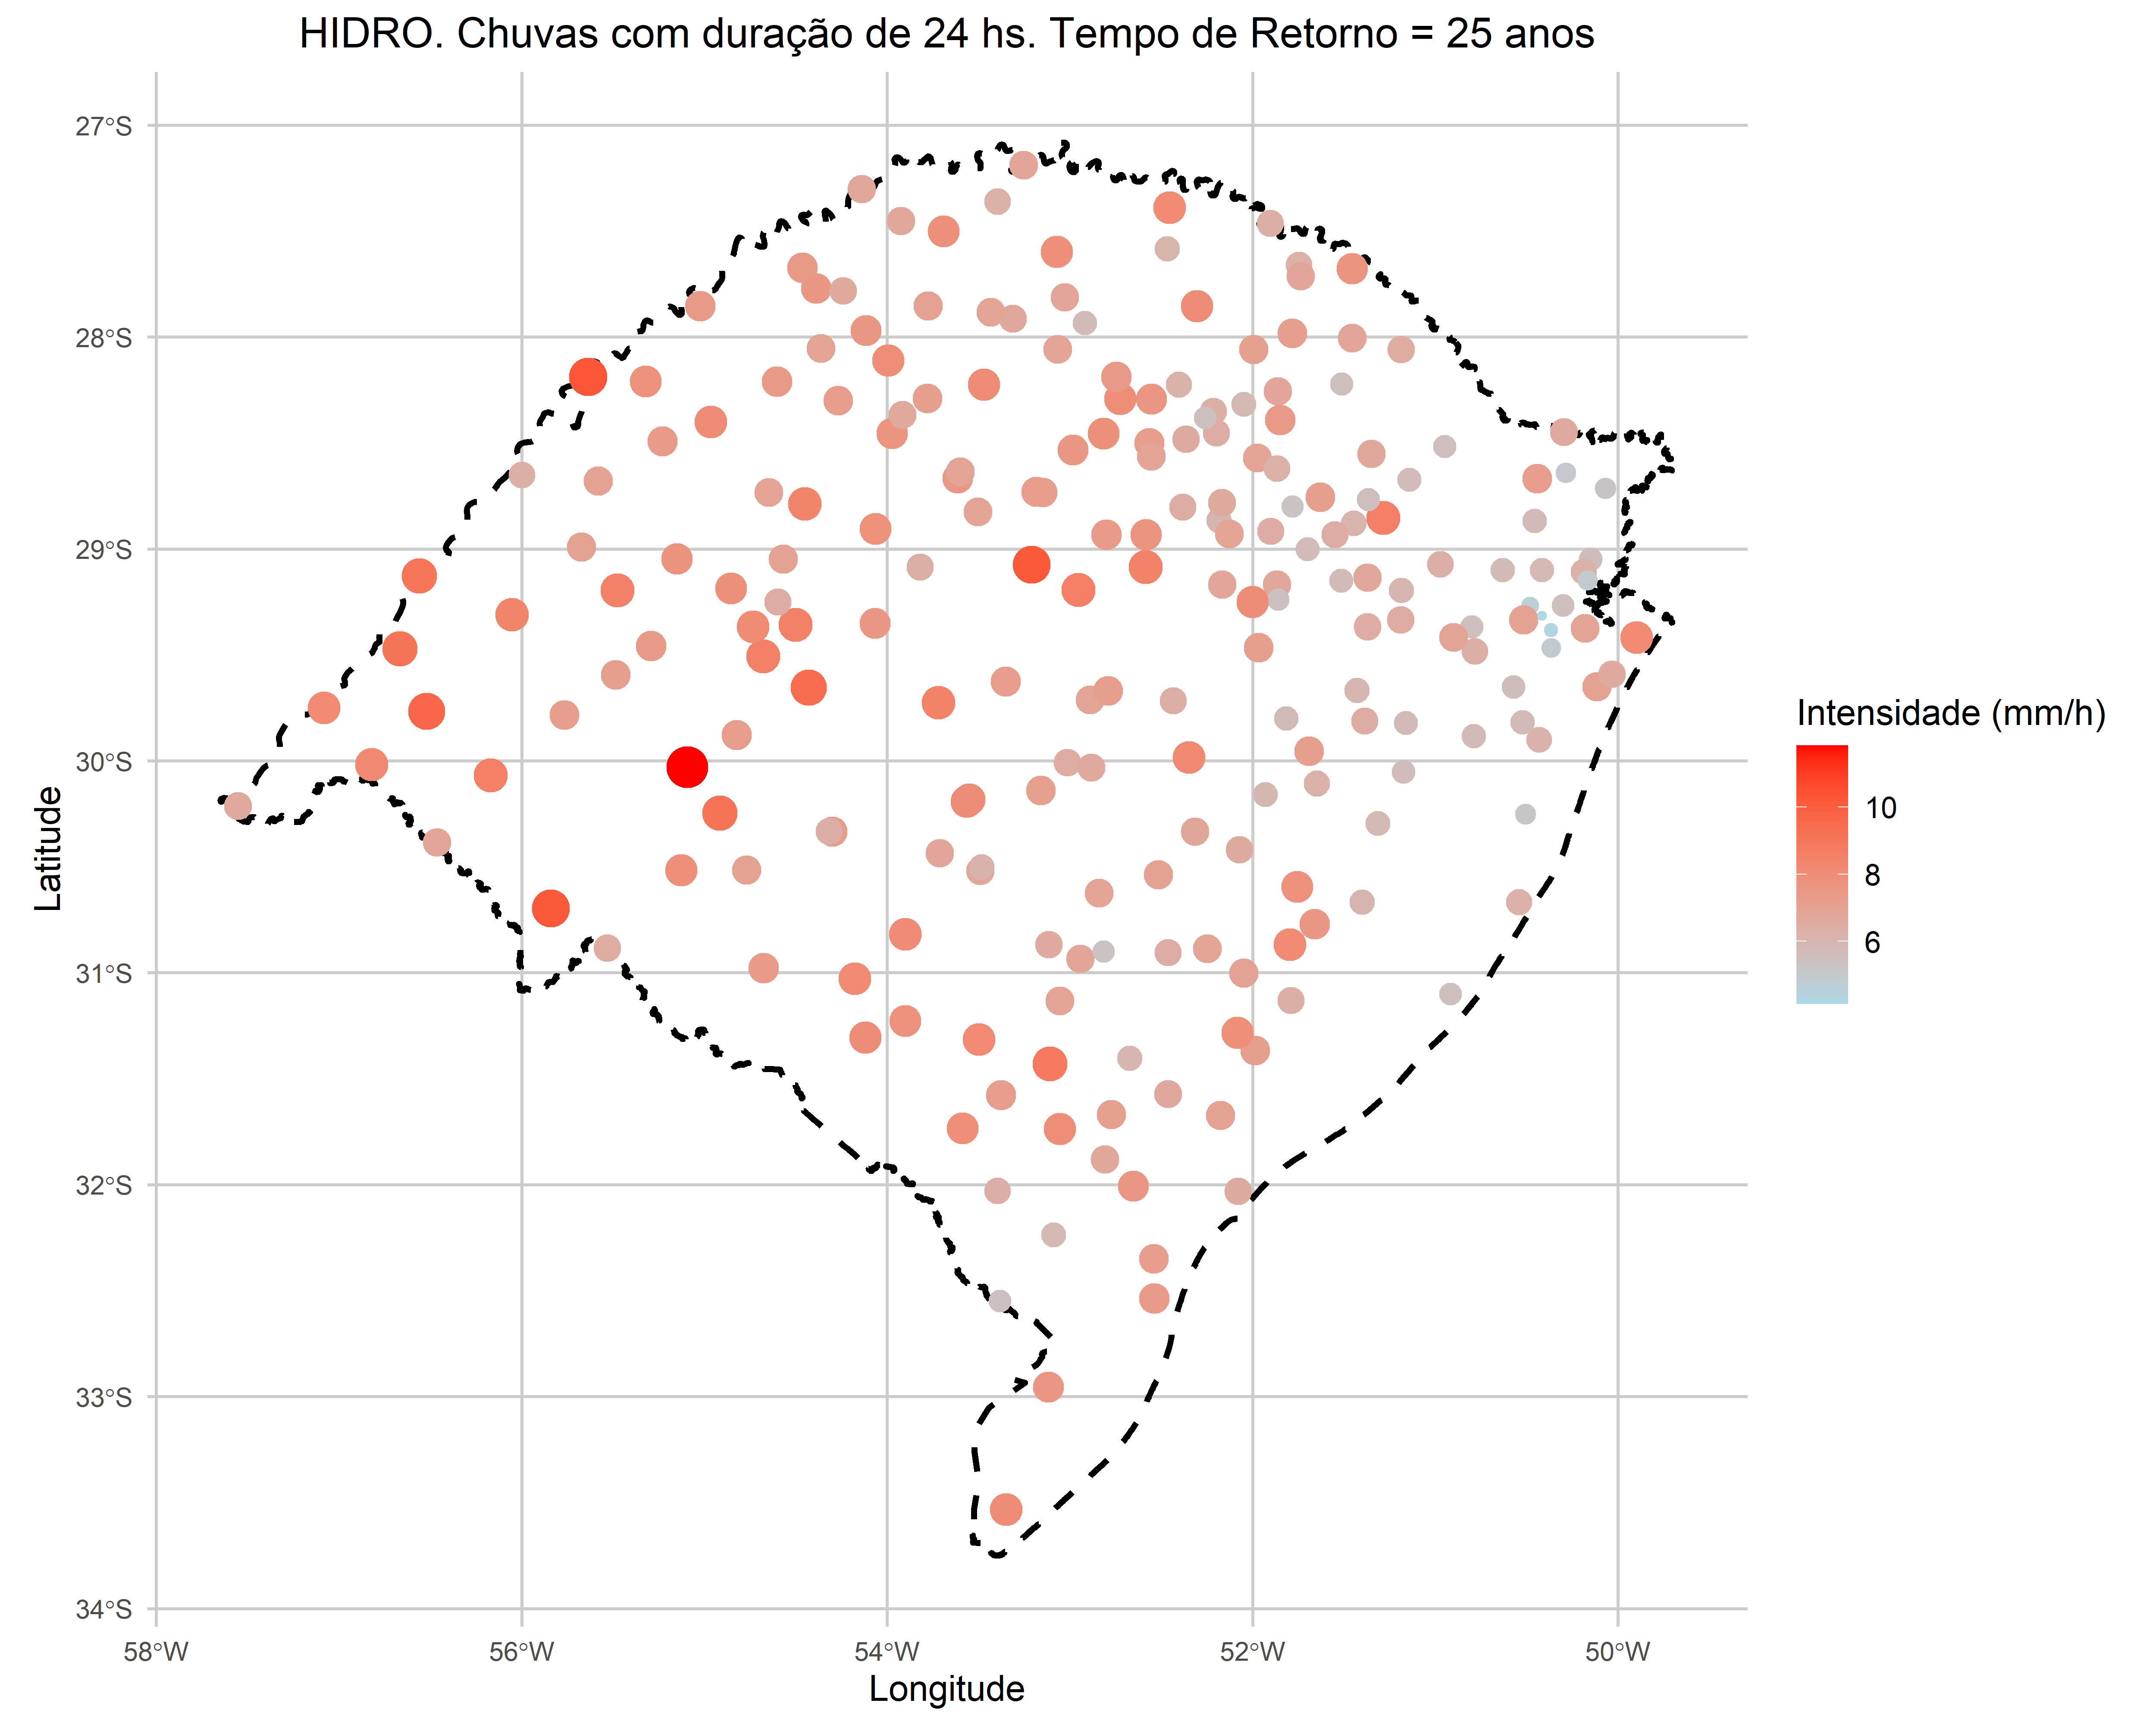
\includegraphics{Figuras/Figura5a.png}

}

\subcaption{\label{fig-Figura5a}Base de dados HIDRO}

\end{minipage}%
\newline
\begin{minipage}{\linewidth}

\centering{

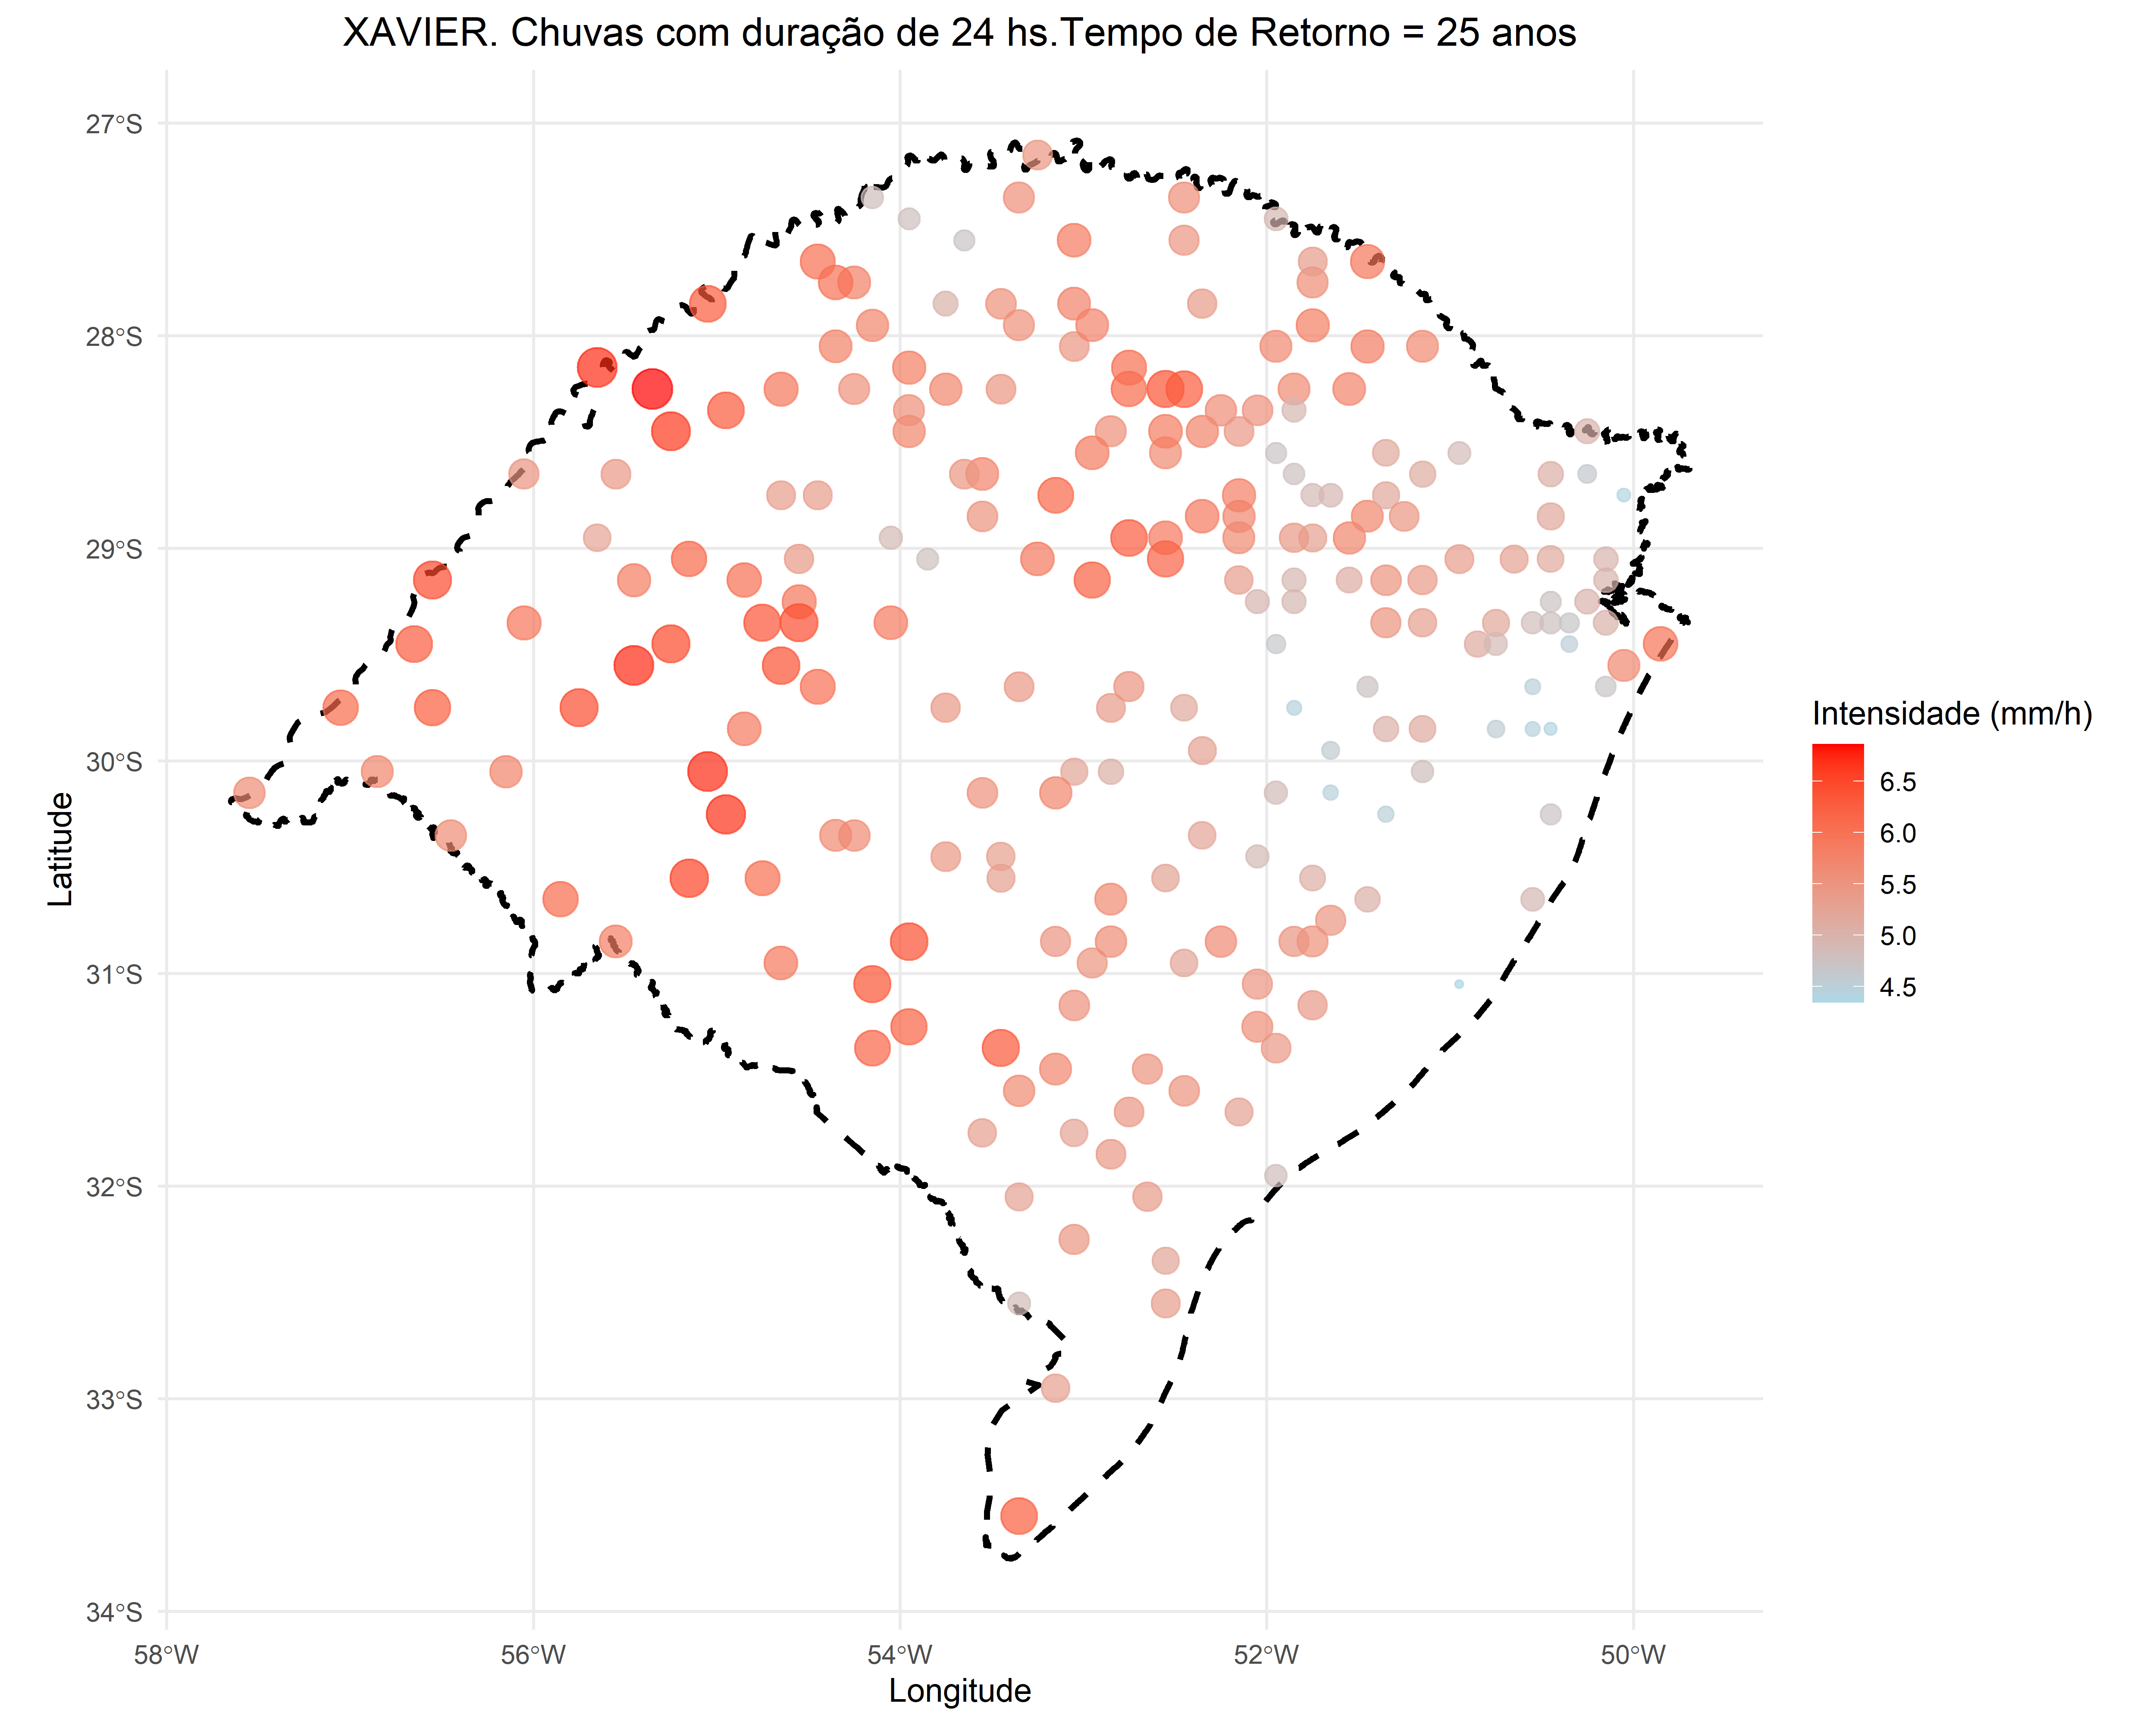
\includegraphics{Figuras/Figura5b.png}

}

\subcaption{\label{fig-Figura5b}Base de dados XAVIER}

\end{minipage}%
\newline
\begin{minipage}{\linewidth}

\centering{

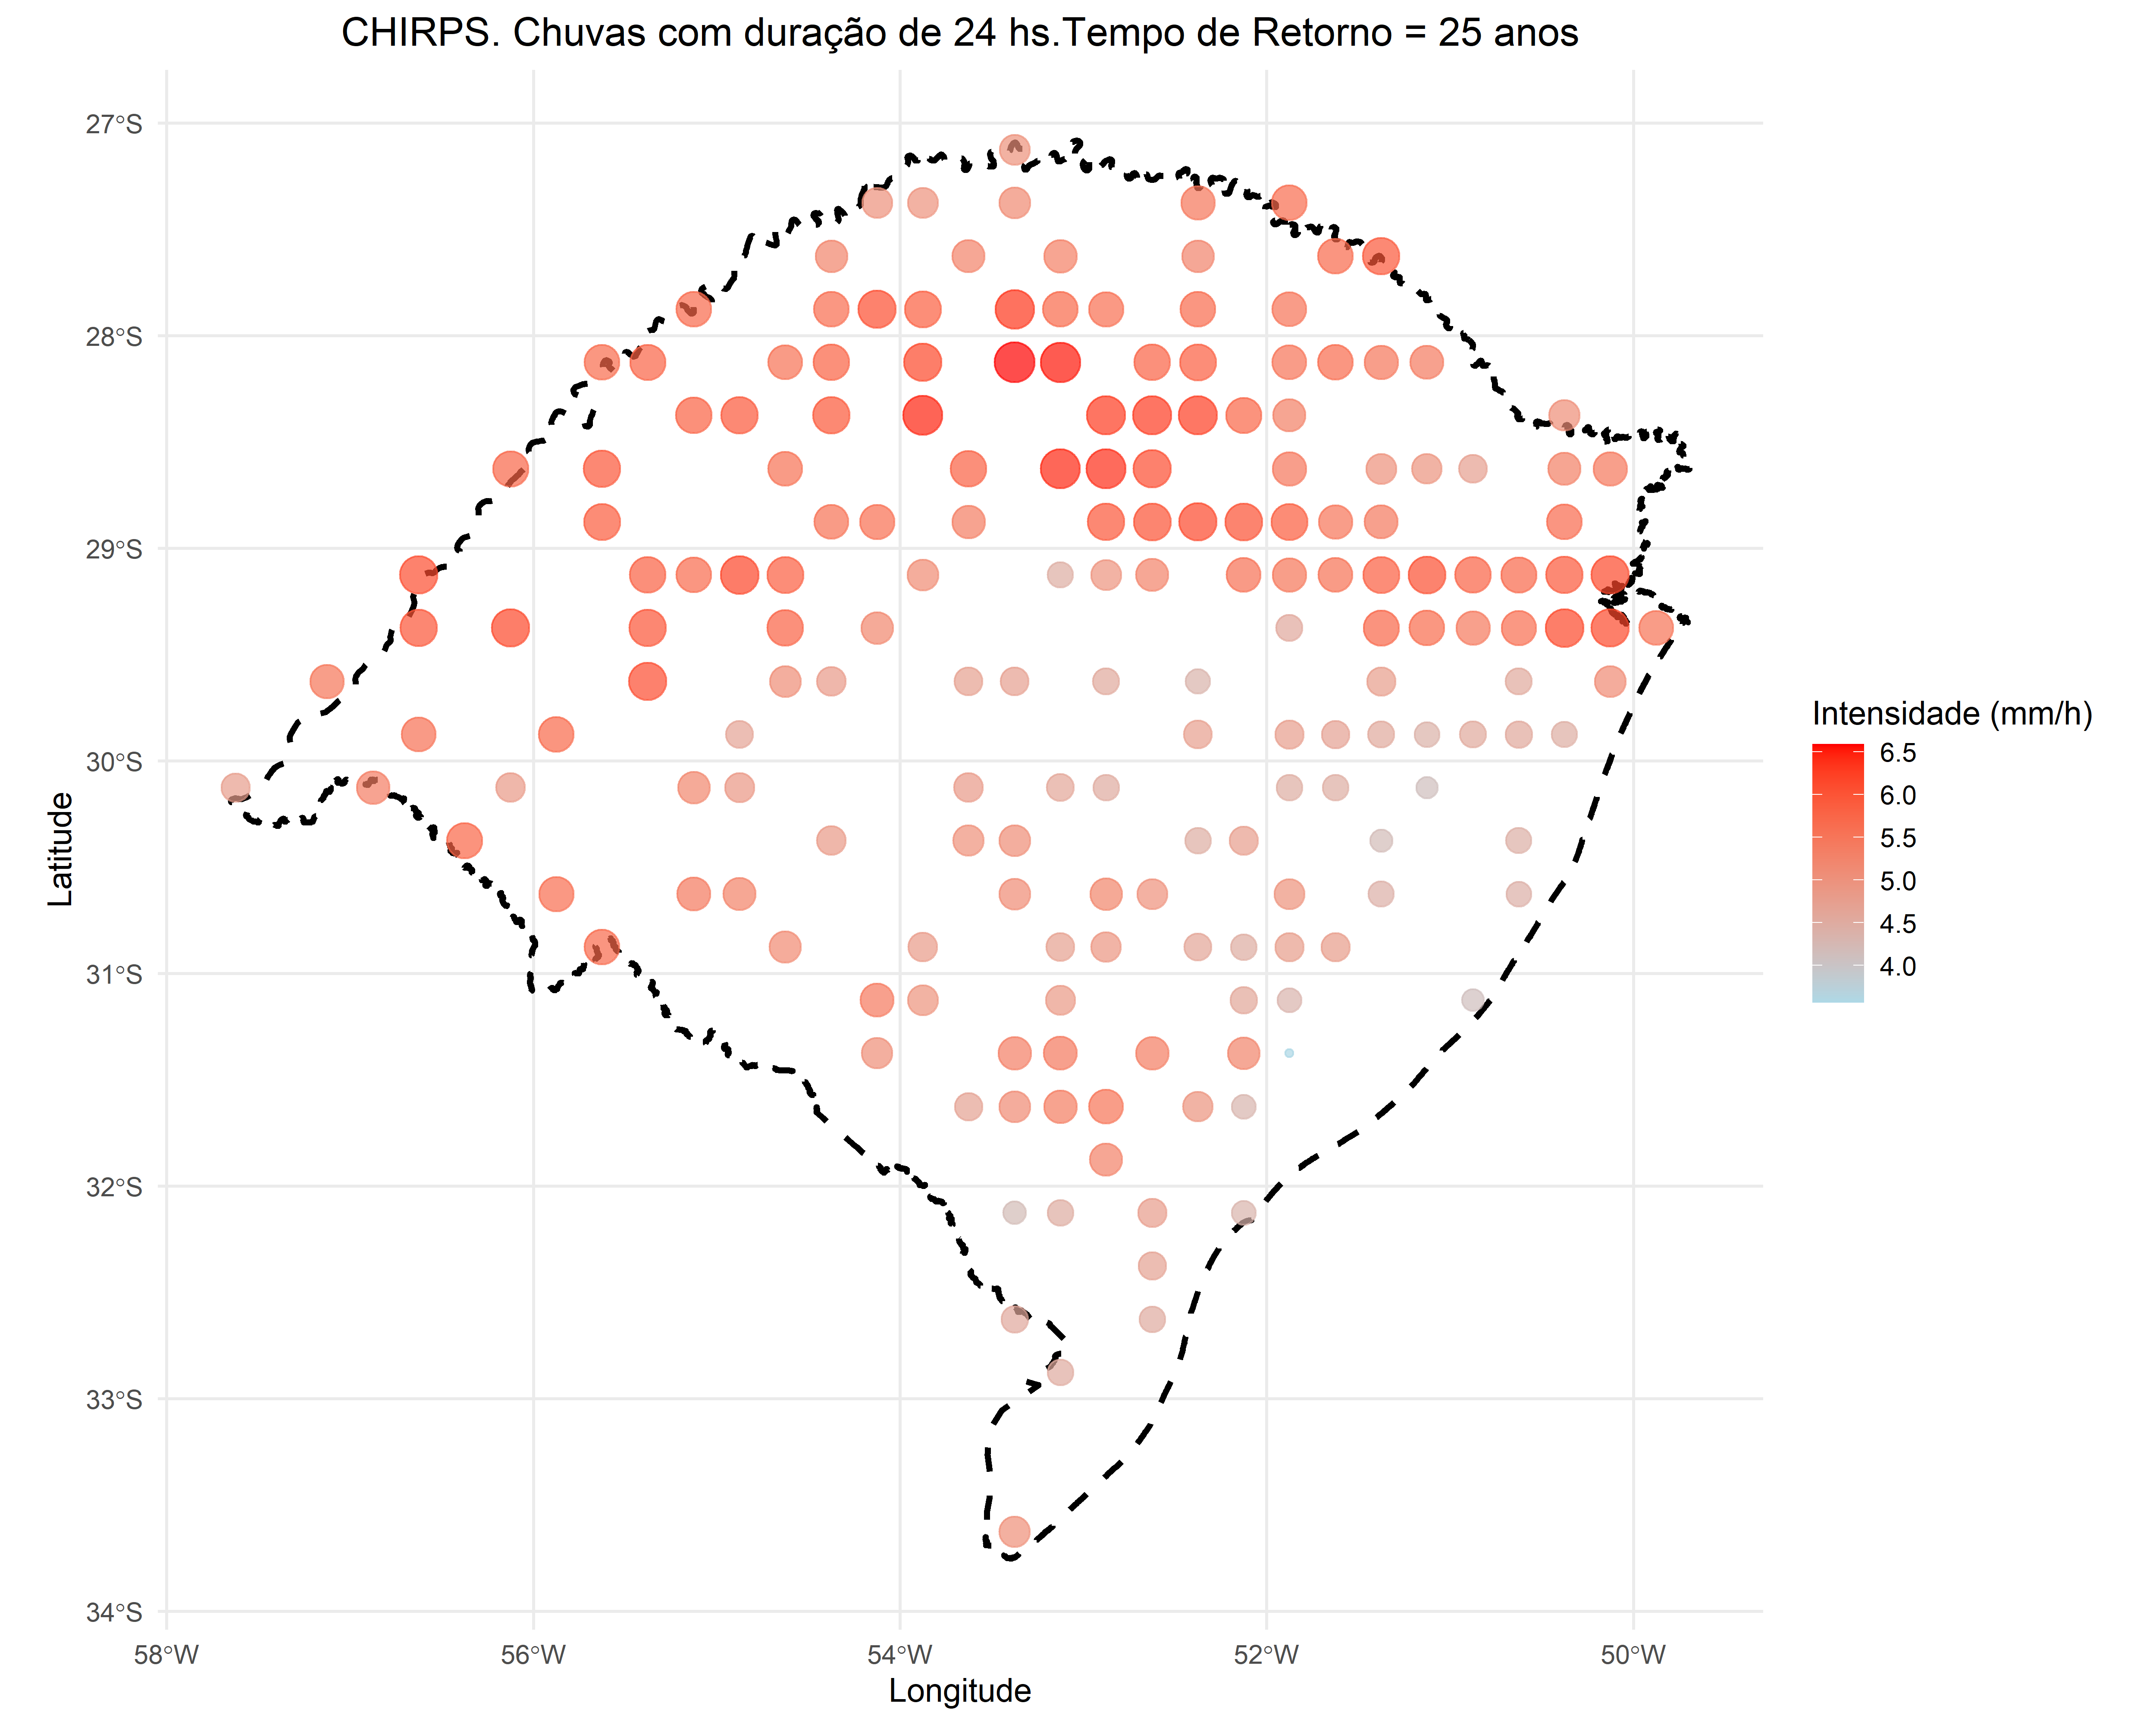
\includegraphics{Figuras/Figura5c.png}

}

\subcaption{\label{fig-Figura5c}Base de dados CHIRPS}

\end{minipage}%

\caption{\label{fig-Figura5}Magnitude da intensidade da precipitação com
duração de 24 horas para o tempo de retorno de 25 anos considerando a
base de dados HDIRO (a); XAVIER (b) e CHIRPS (c). O tamanho dos circulos
azuis indica a magnitude da intensidade das chuvas.}

\end{figure}%

\begin{figure}

\begin{minipage}{\linewidth}

\centering{

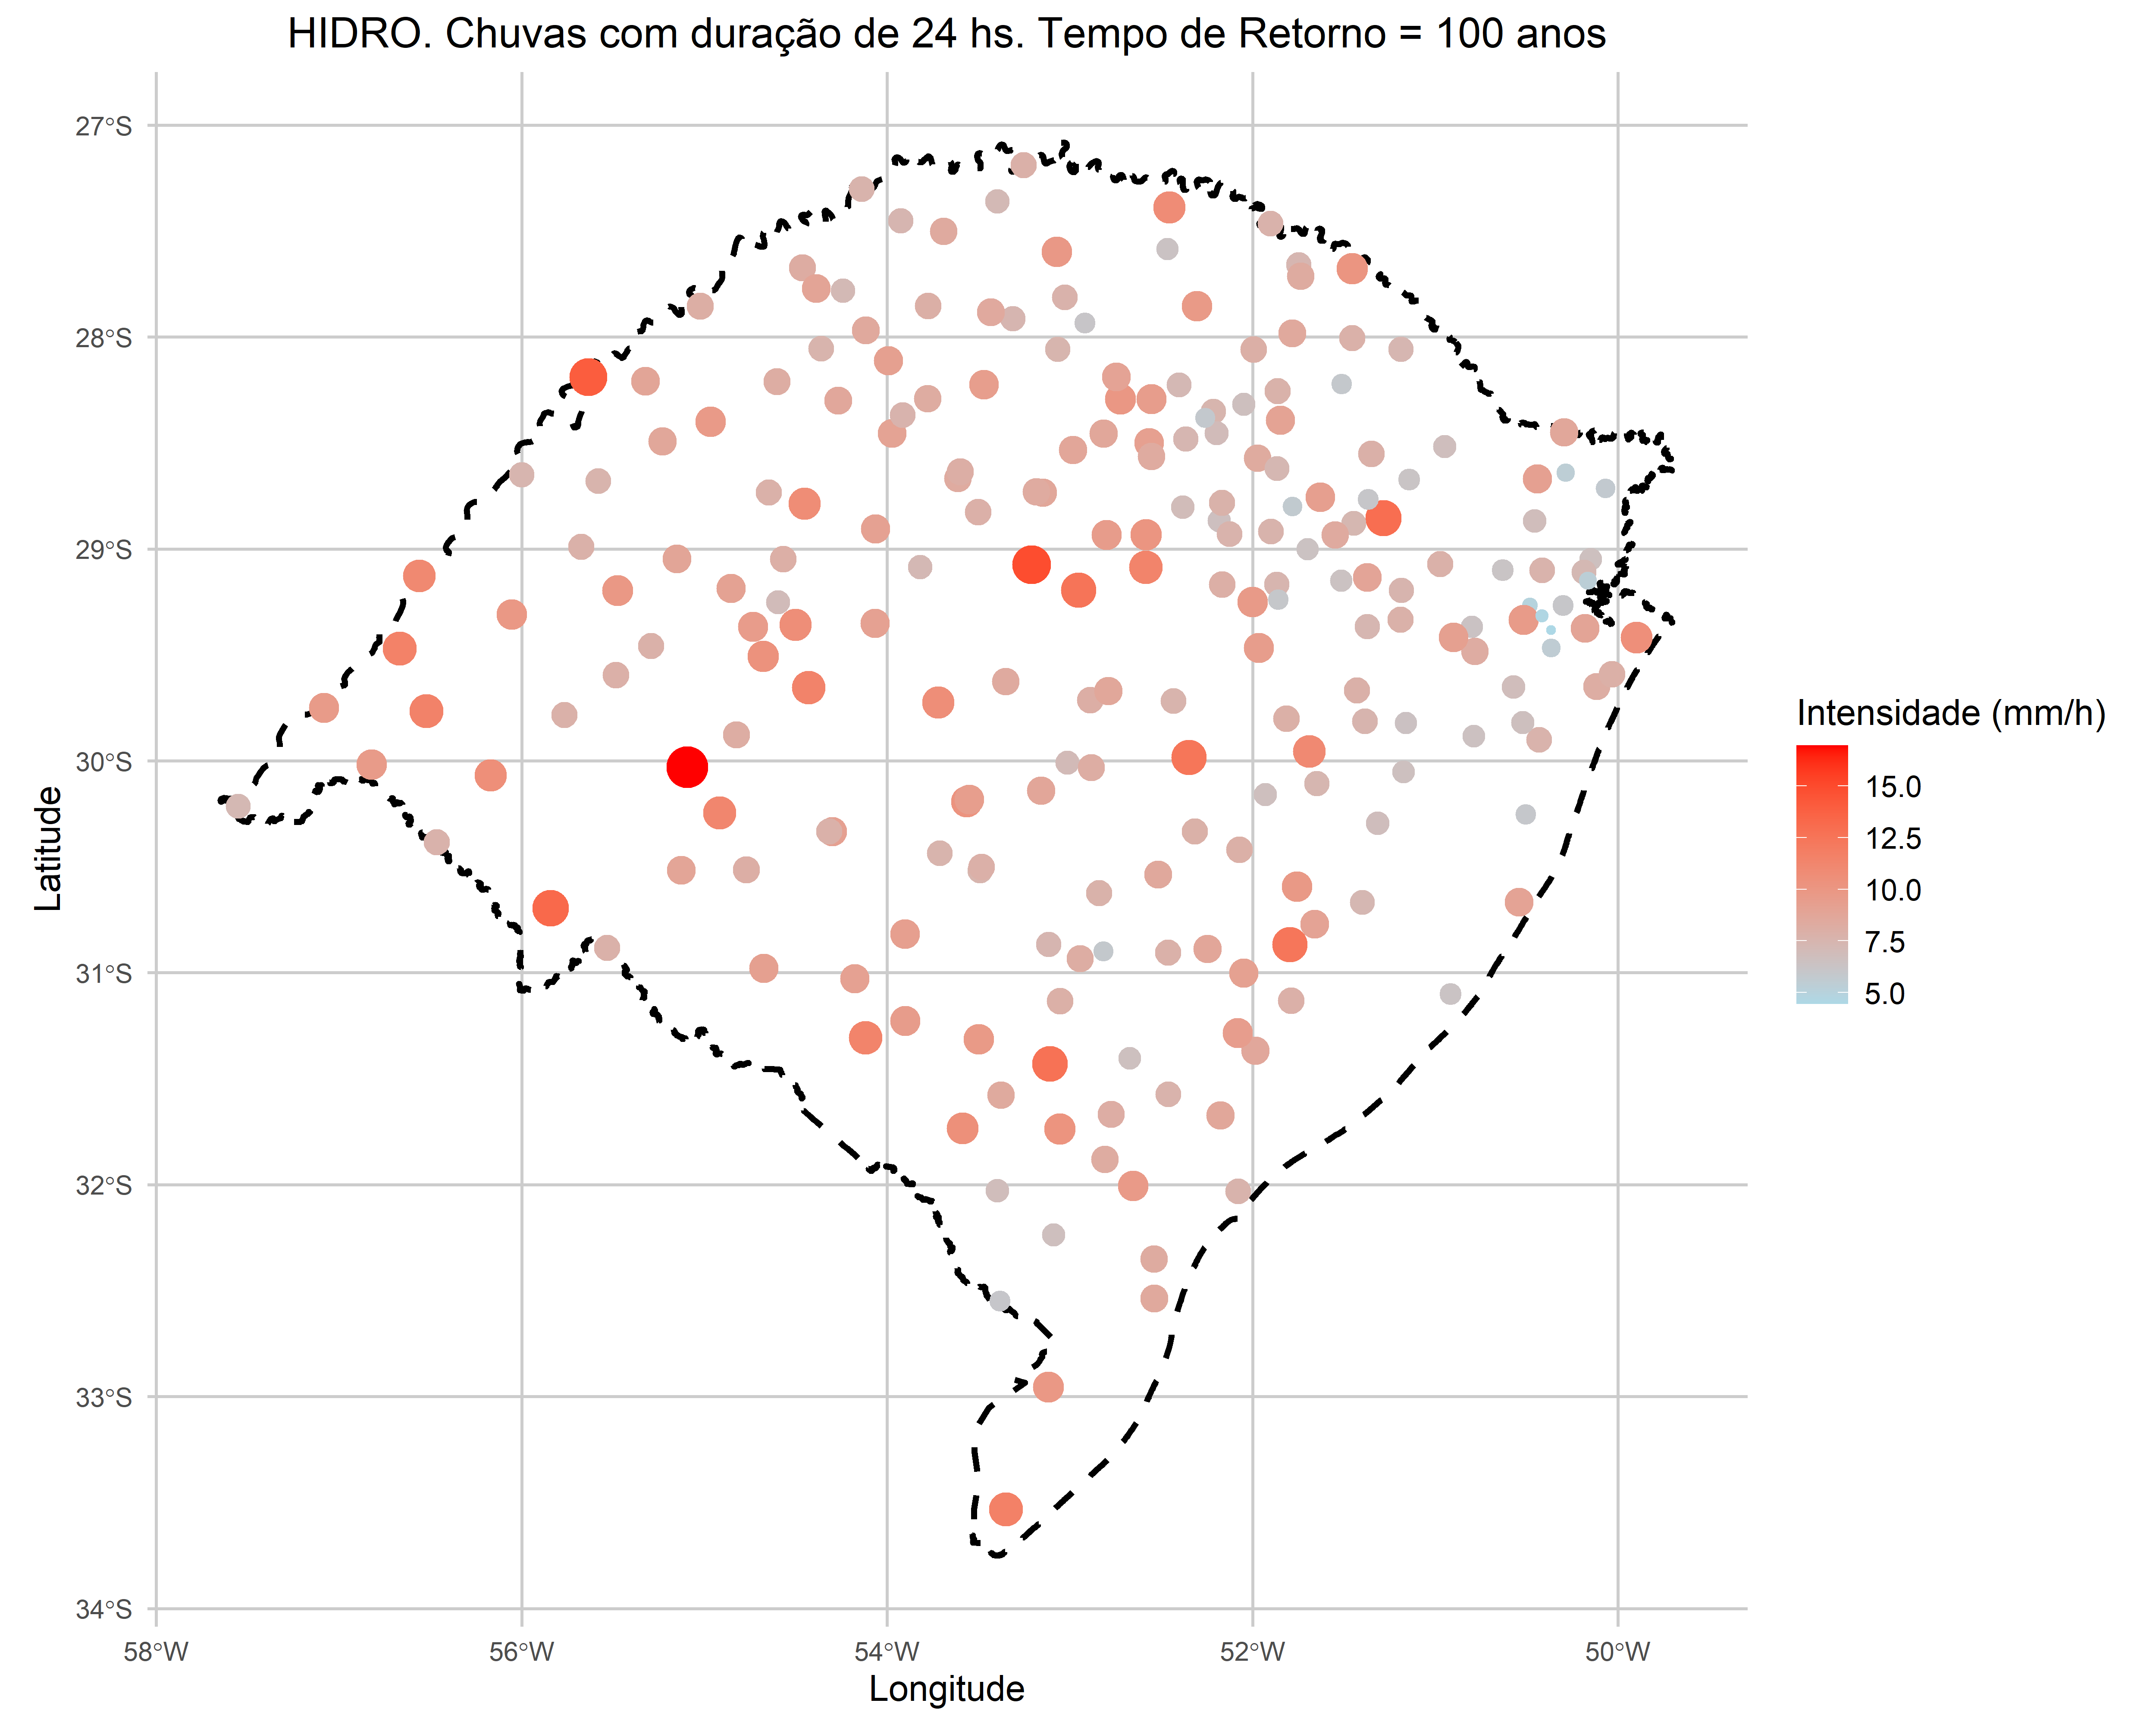
\includegraphics{Figuras/Figura6a.png}

}

\subcaption{\label{fig-Figura6a}Base de dados HIDRO}

\end{minipage}%
\newline
\begin{minipage}{\linewidth}

\centering{

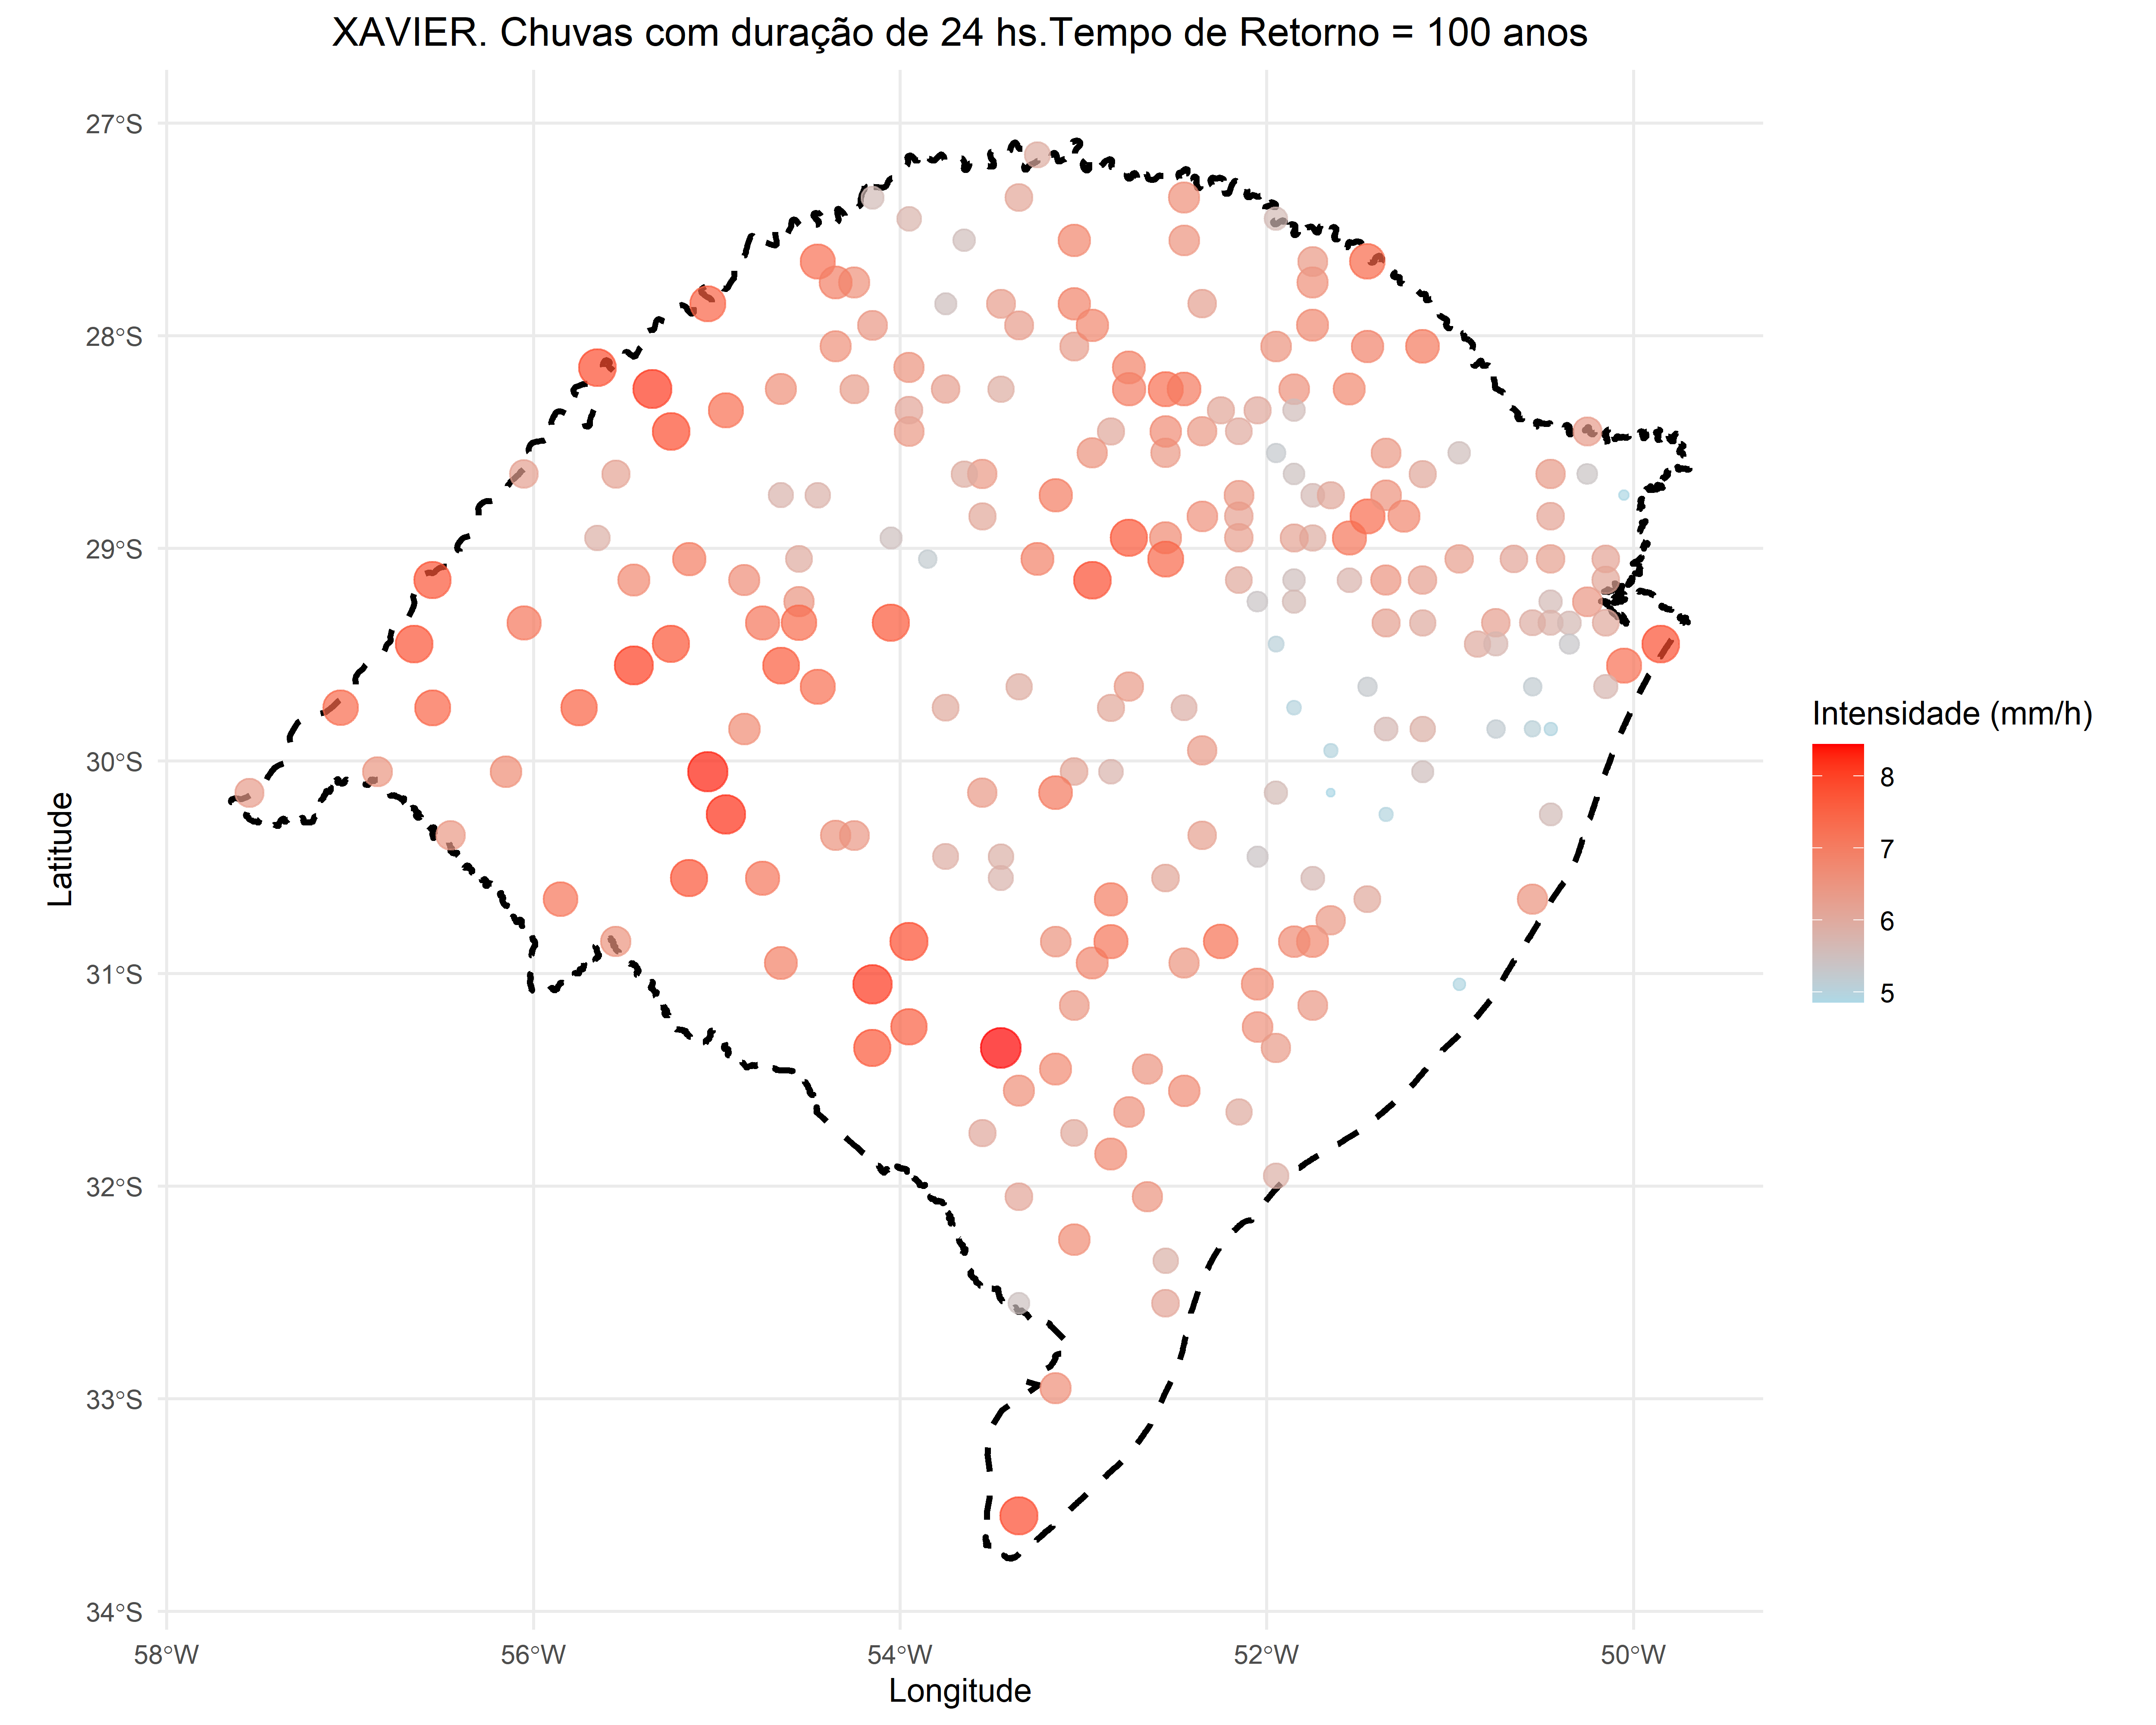
\includegraphics{Figuras/Figura6b.png}

}

\subcaption{\label{fig-Figura6b}Base de dados XAVIER}

\end{minipage}%
\newline
\begin{minipage}{\linewidth}

\centering{

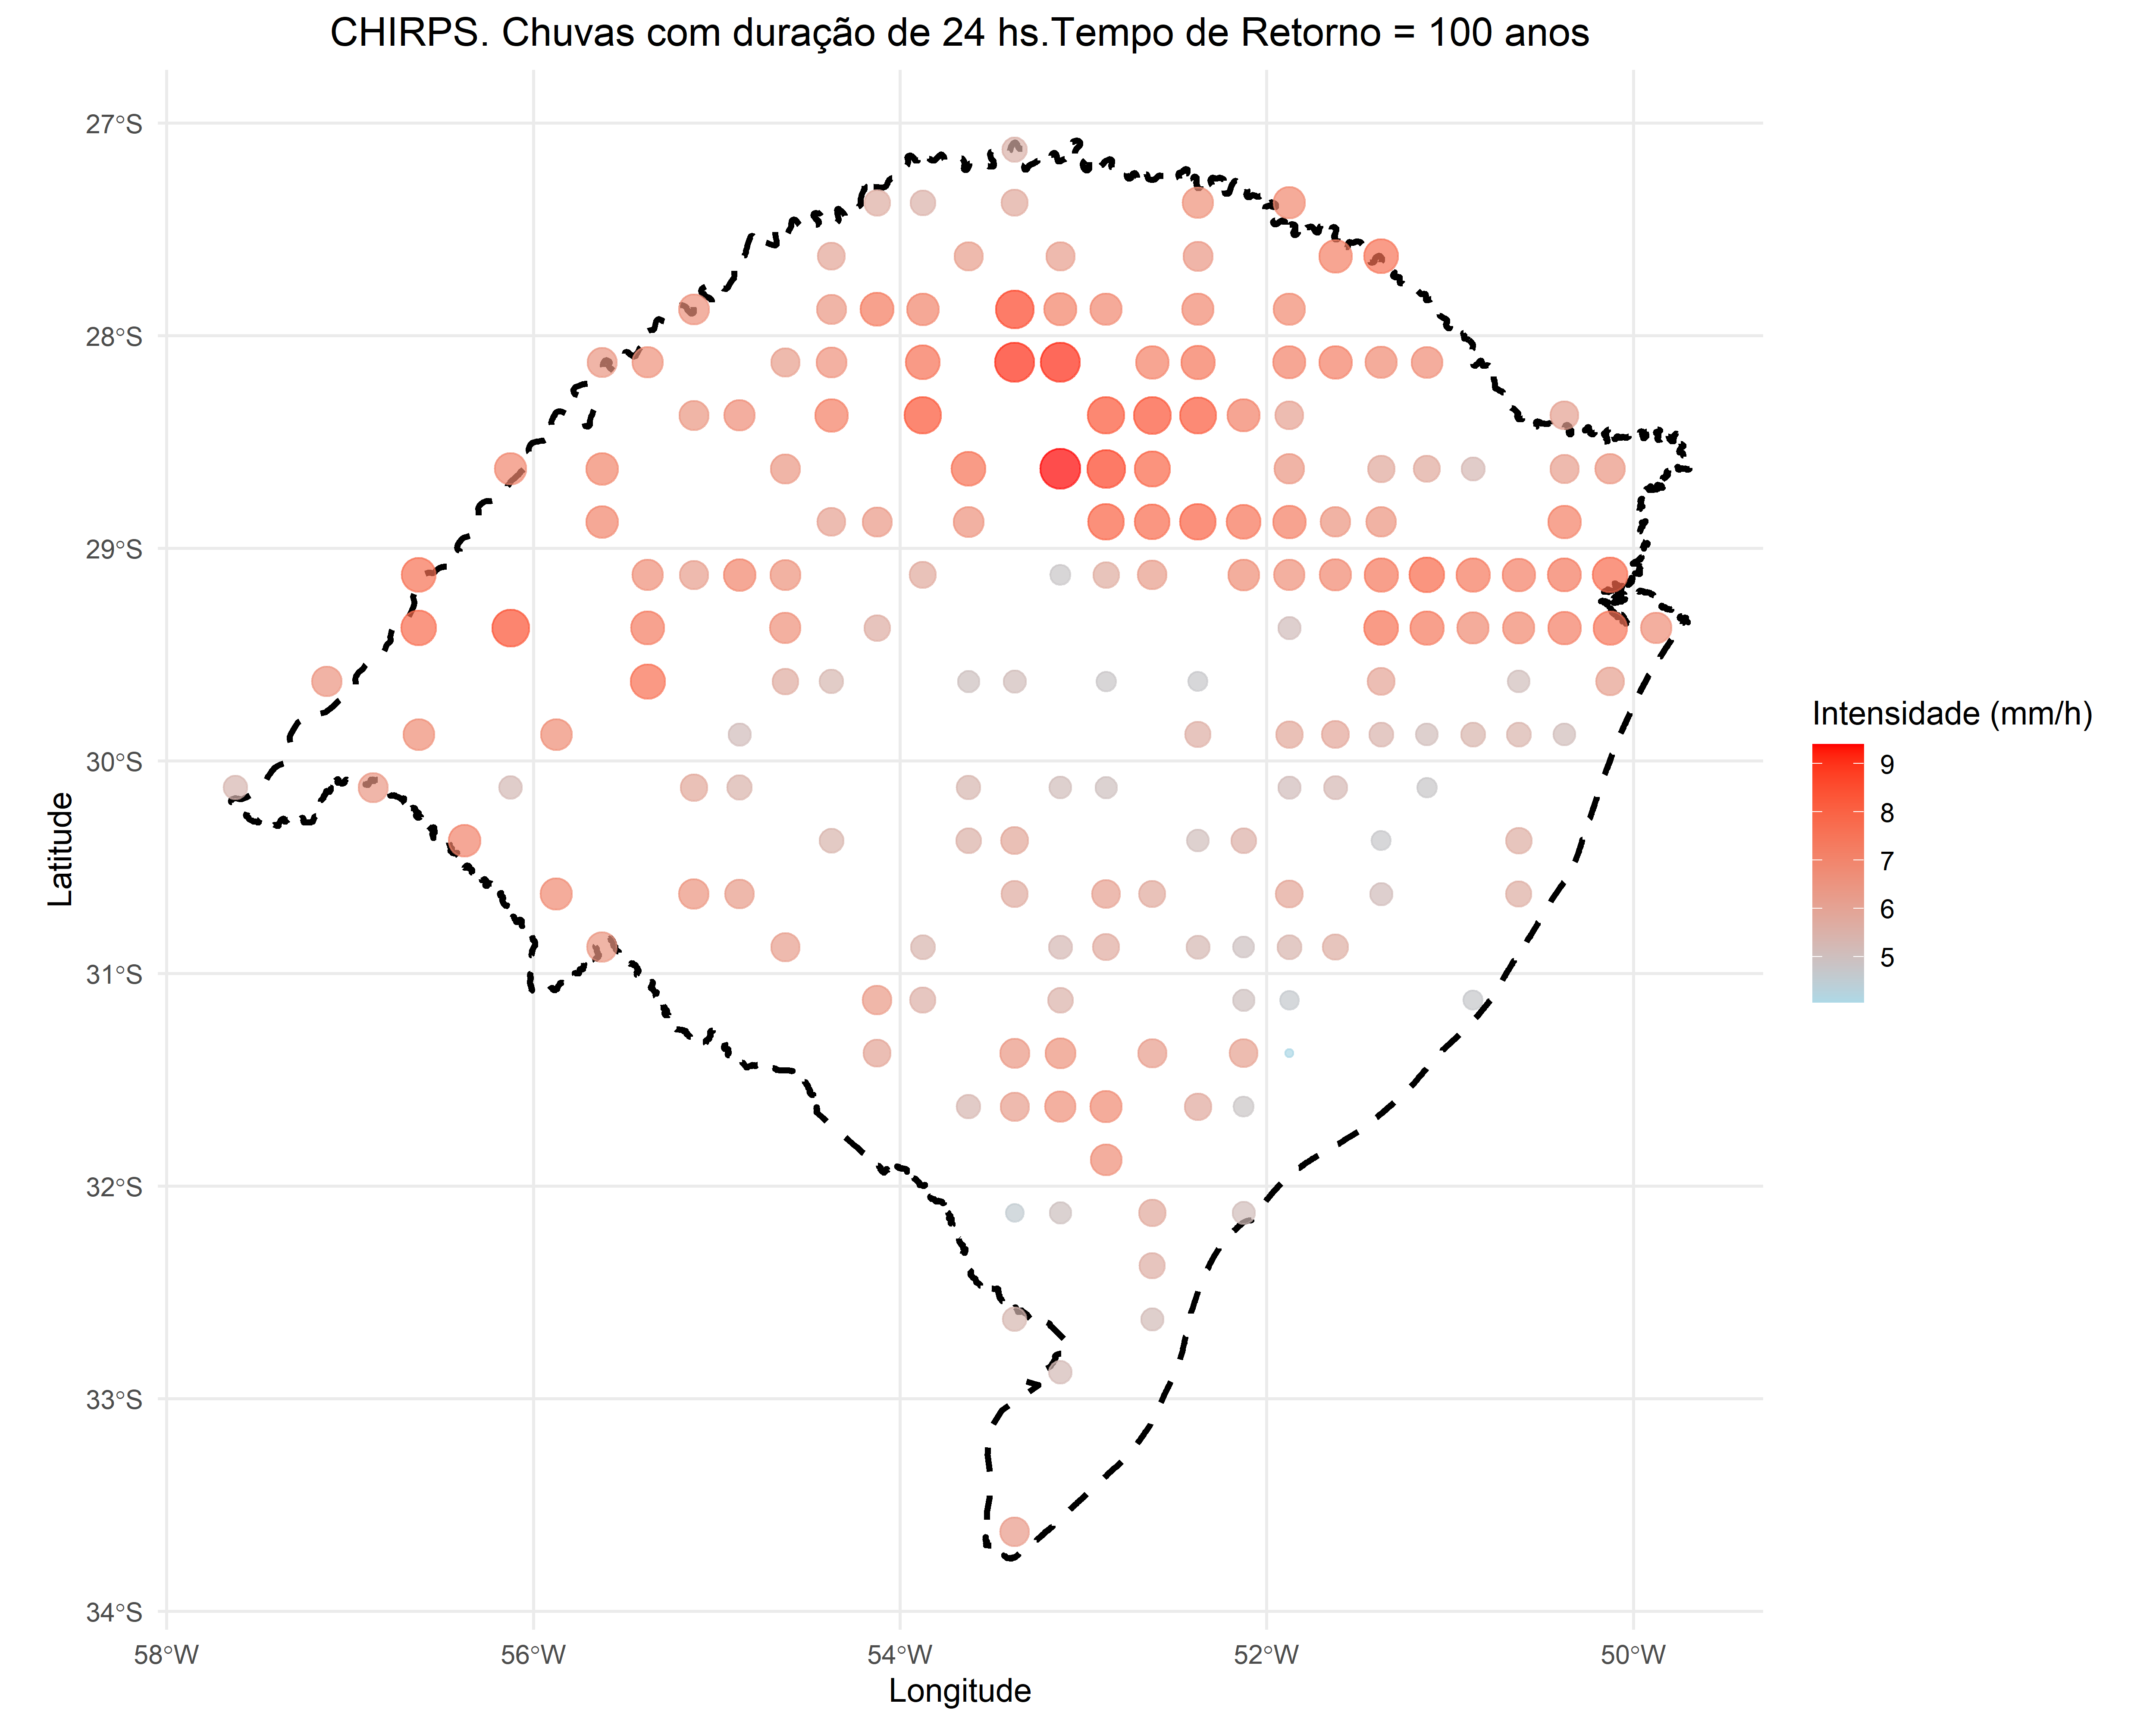
\includegraphics{Figuras/Figura6c.png}

}

\subcaption{\label{fig-Figura6c}Base de dados CHIRPS}

\end{minipage}%

\caption{\label{fig-Figura6}Magnitude da intensidade da precipitação com
duração de 24 horas para o tempo de retorno de 100 anos considerando a
base de dados HDIRO (a); XAVIER (b) e CHIRPS (c). O tamanho dos circulos
azuis indica a magnitude da intensidade das chuvas.}

\end{figure}%

\begin{figure}

\begin{minipage}{\linewidth}

\centering{

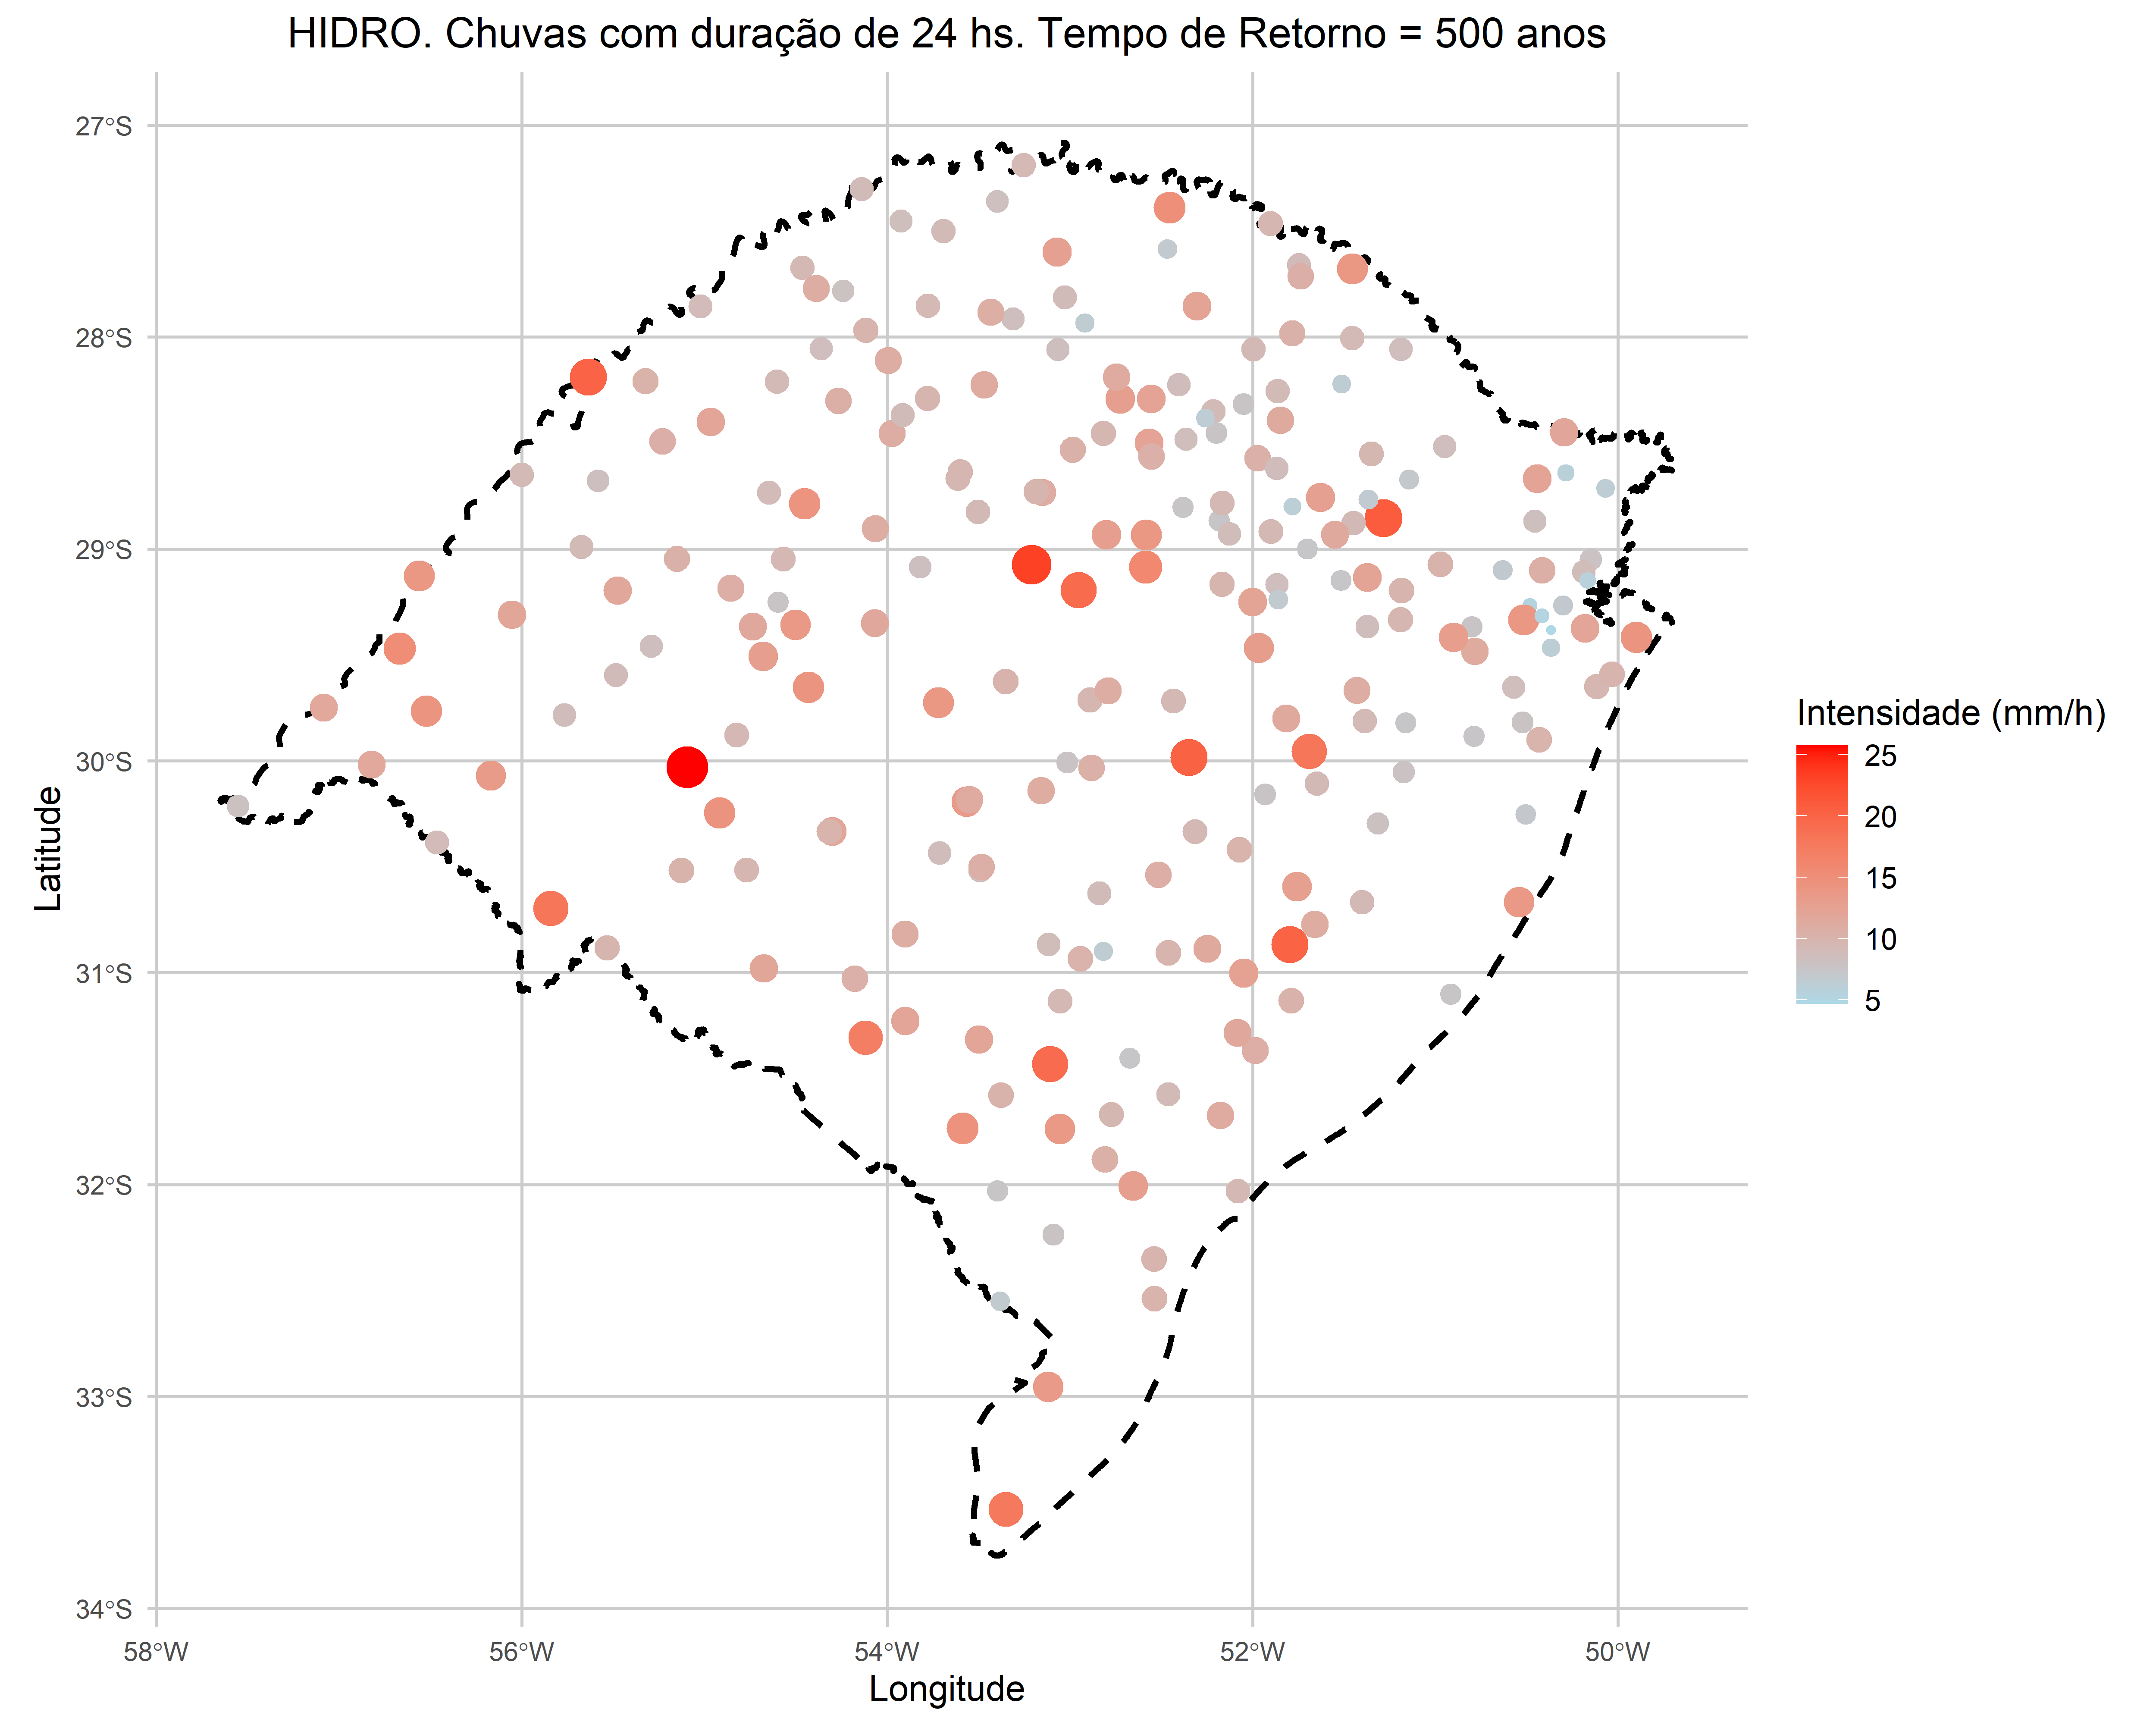
\includegraphics{Figuras/Figura7a.png}

}

\subcaption{\label{fig-Figura7a}Base de dados HIDRO}

\end{minipage}%
\newline
\begin{minipage}{\linewidth}

\centering{

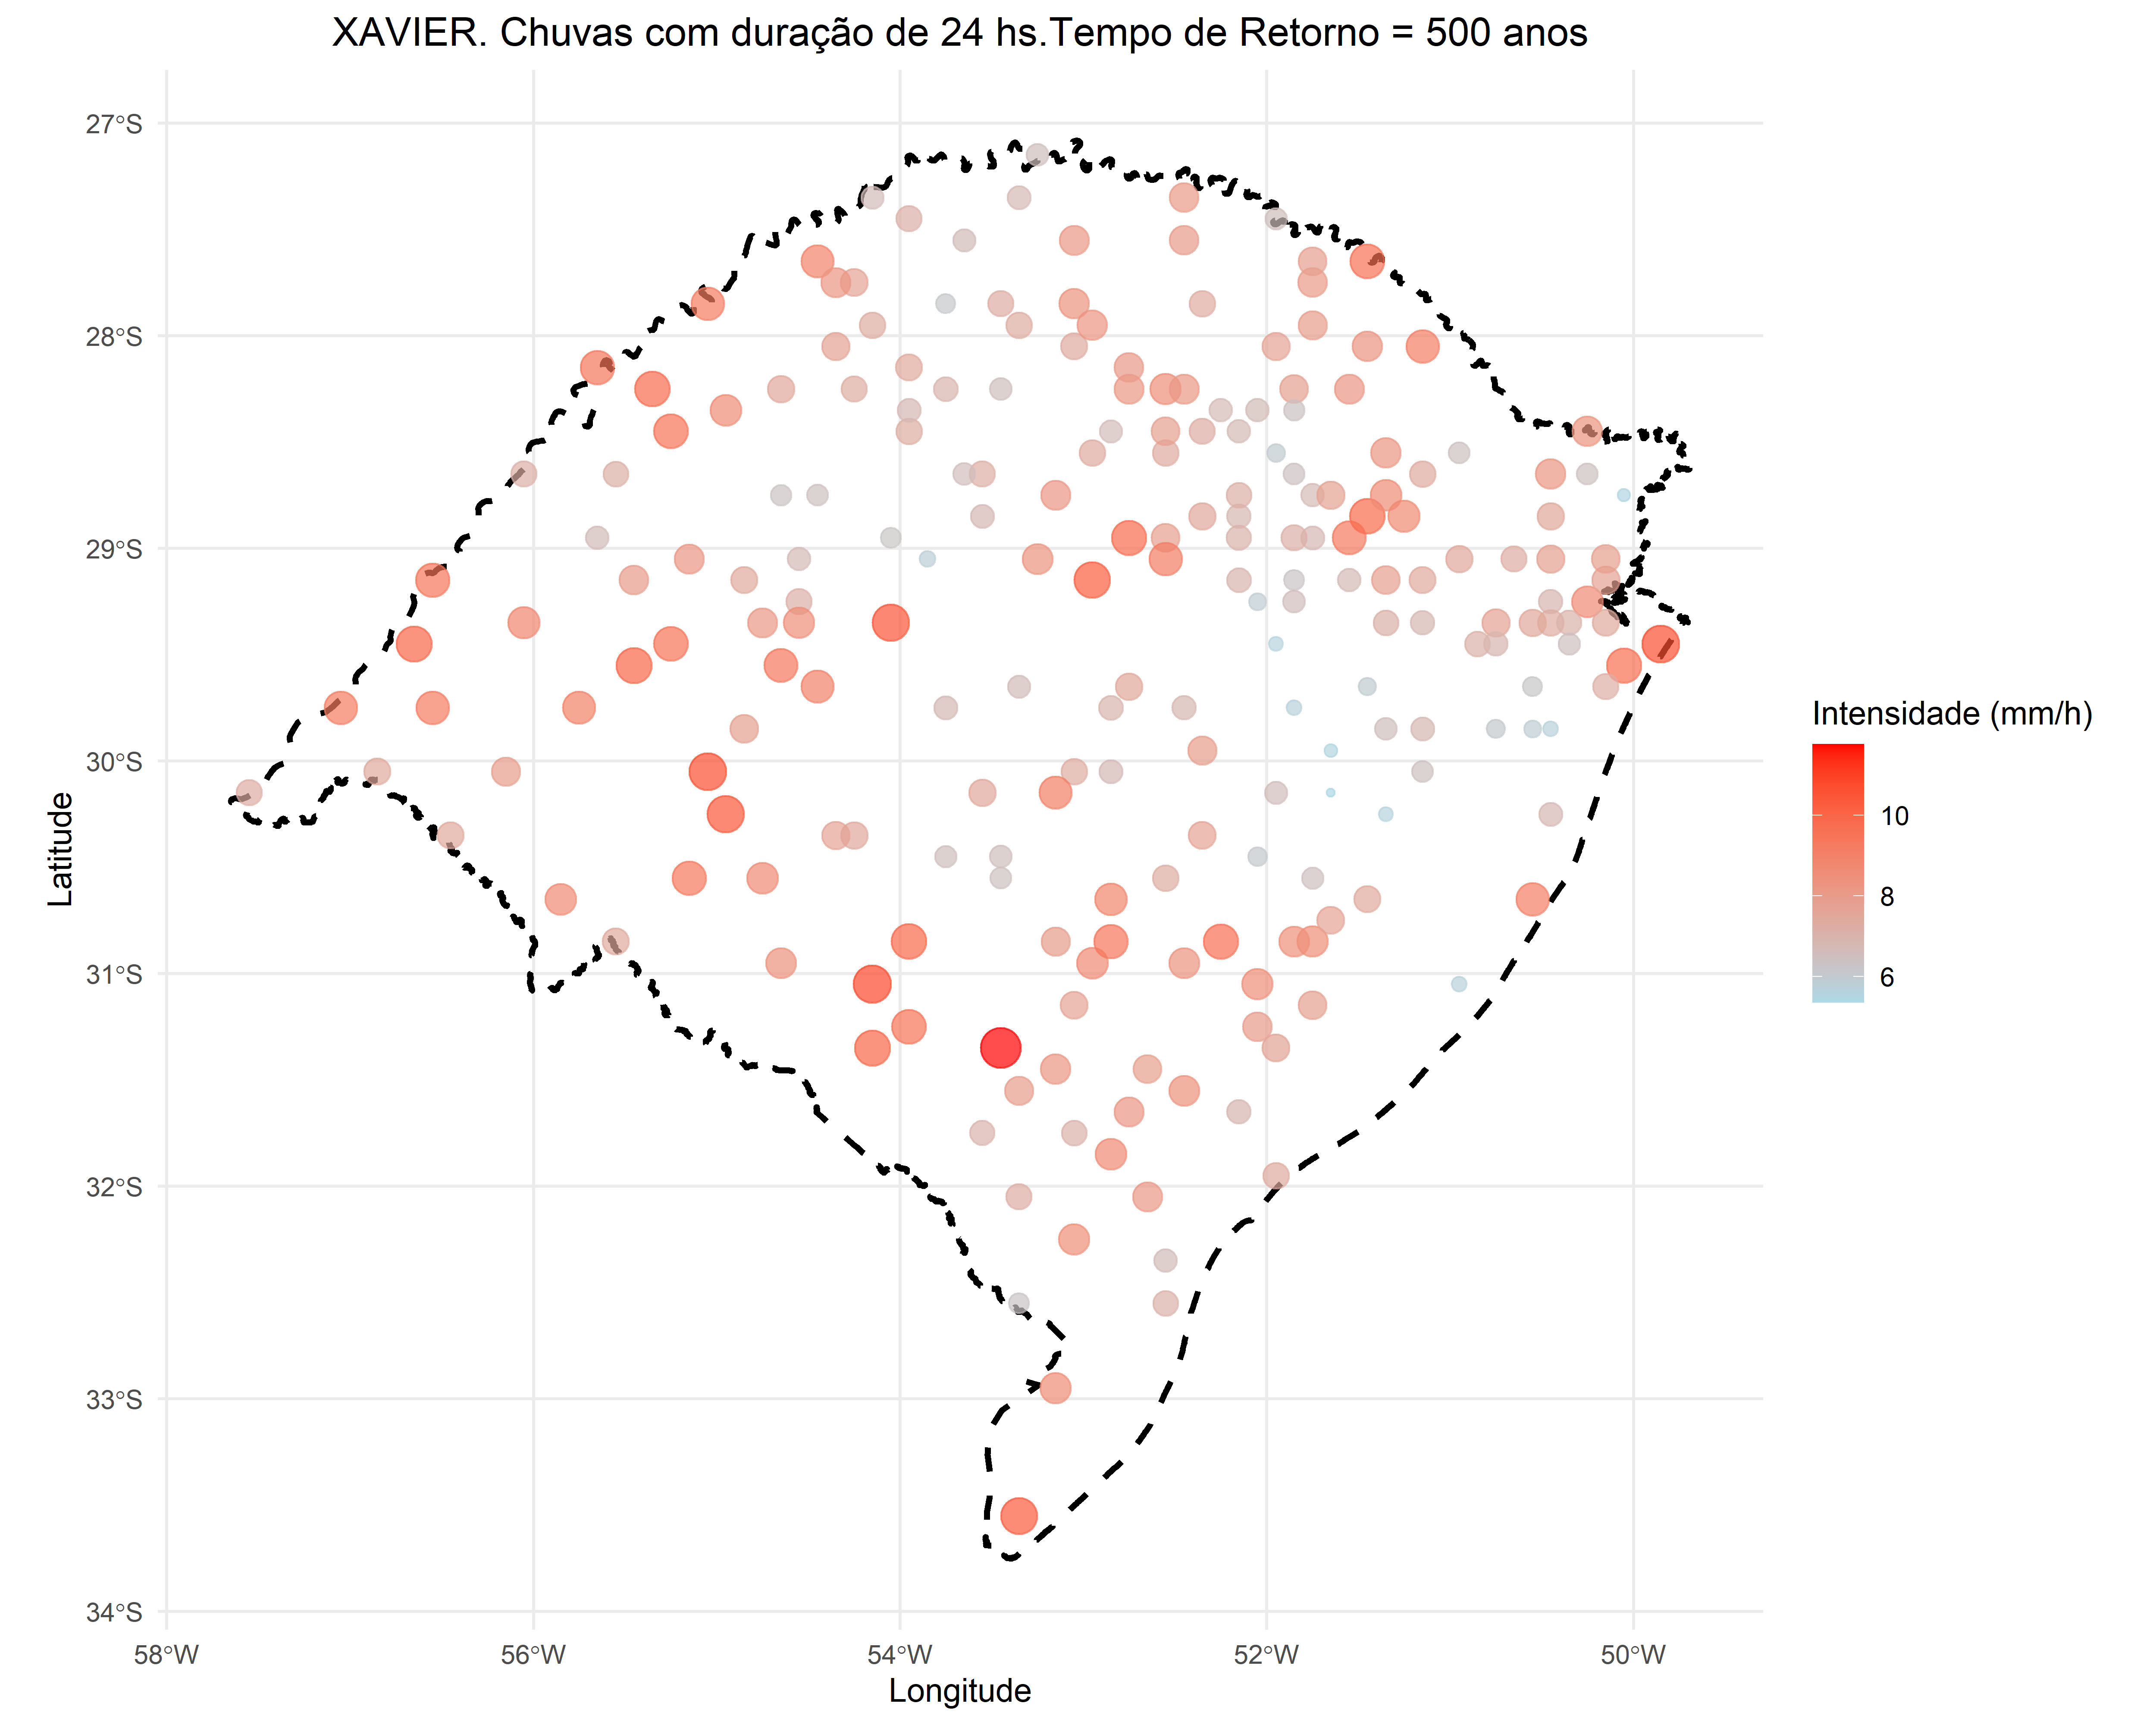
\includegraphics{Figuras/Figura7b.png}

}

\subcaption{\label{fig-Figura7b}Base de dados XAVIER}

\end{minipage}%
\newline
\begin{minipage}{\linewidth}

\centering{

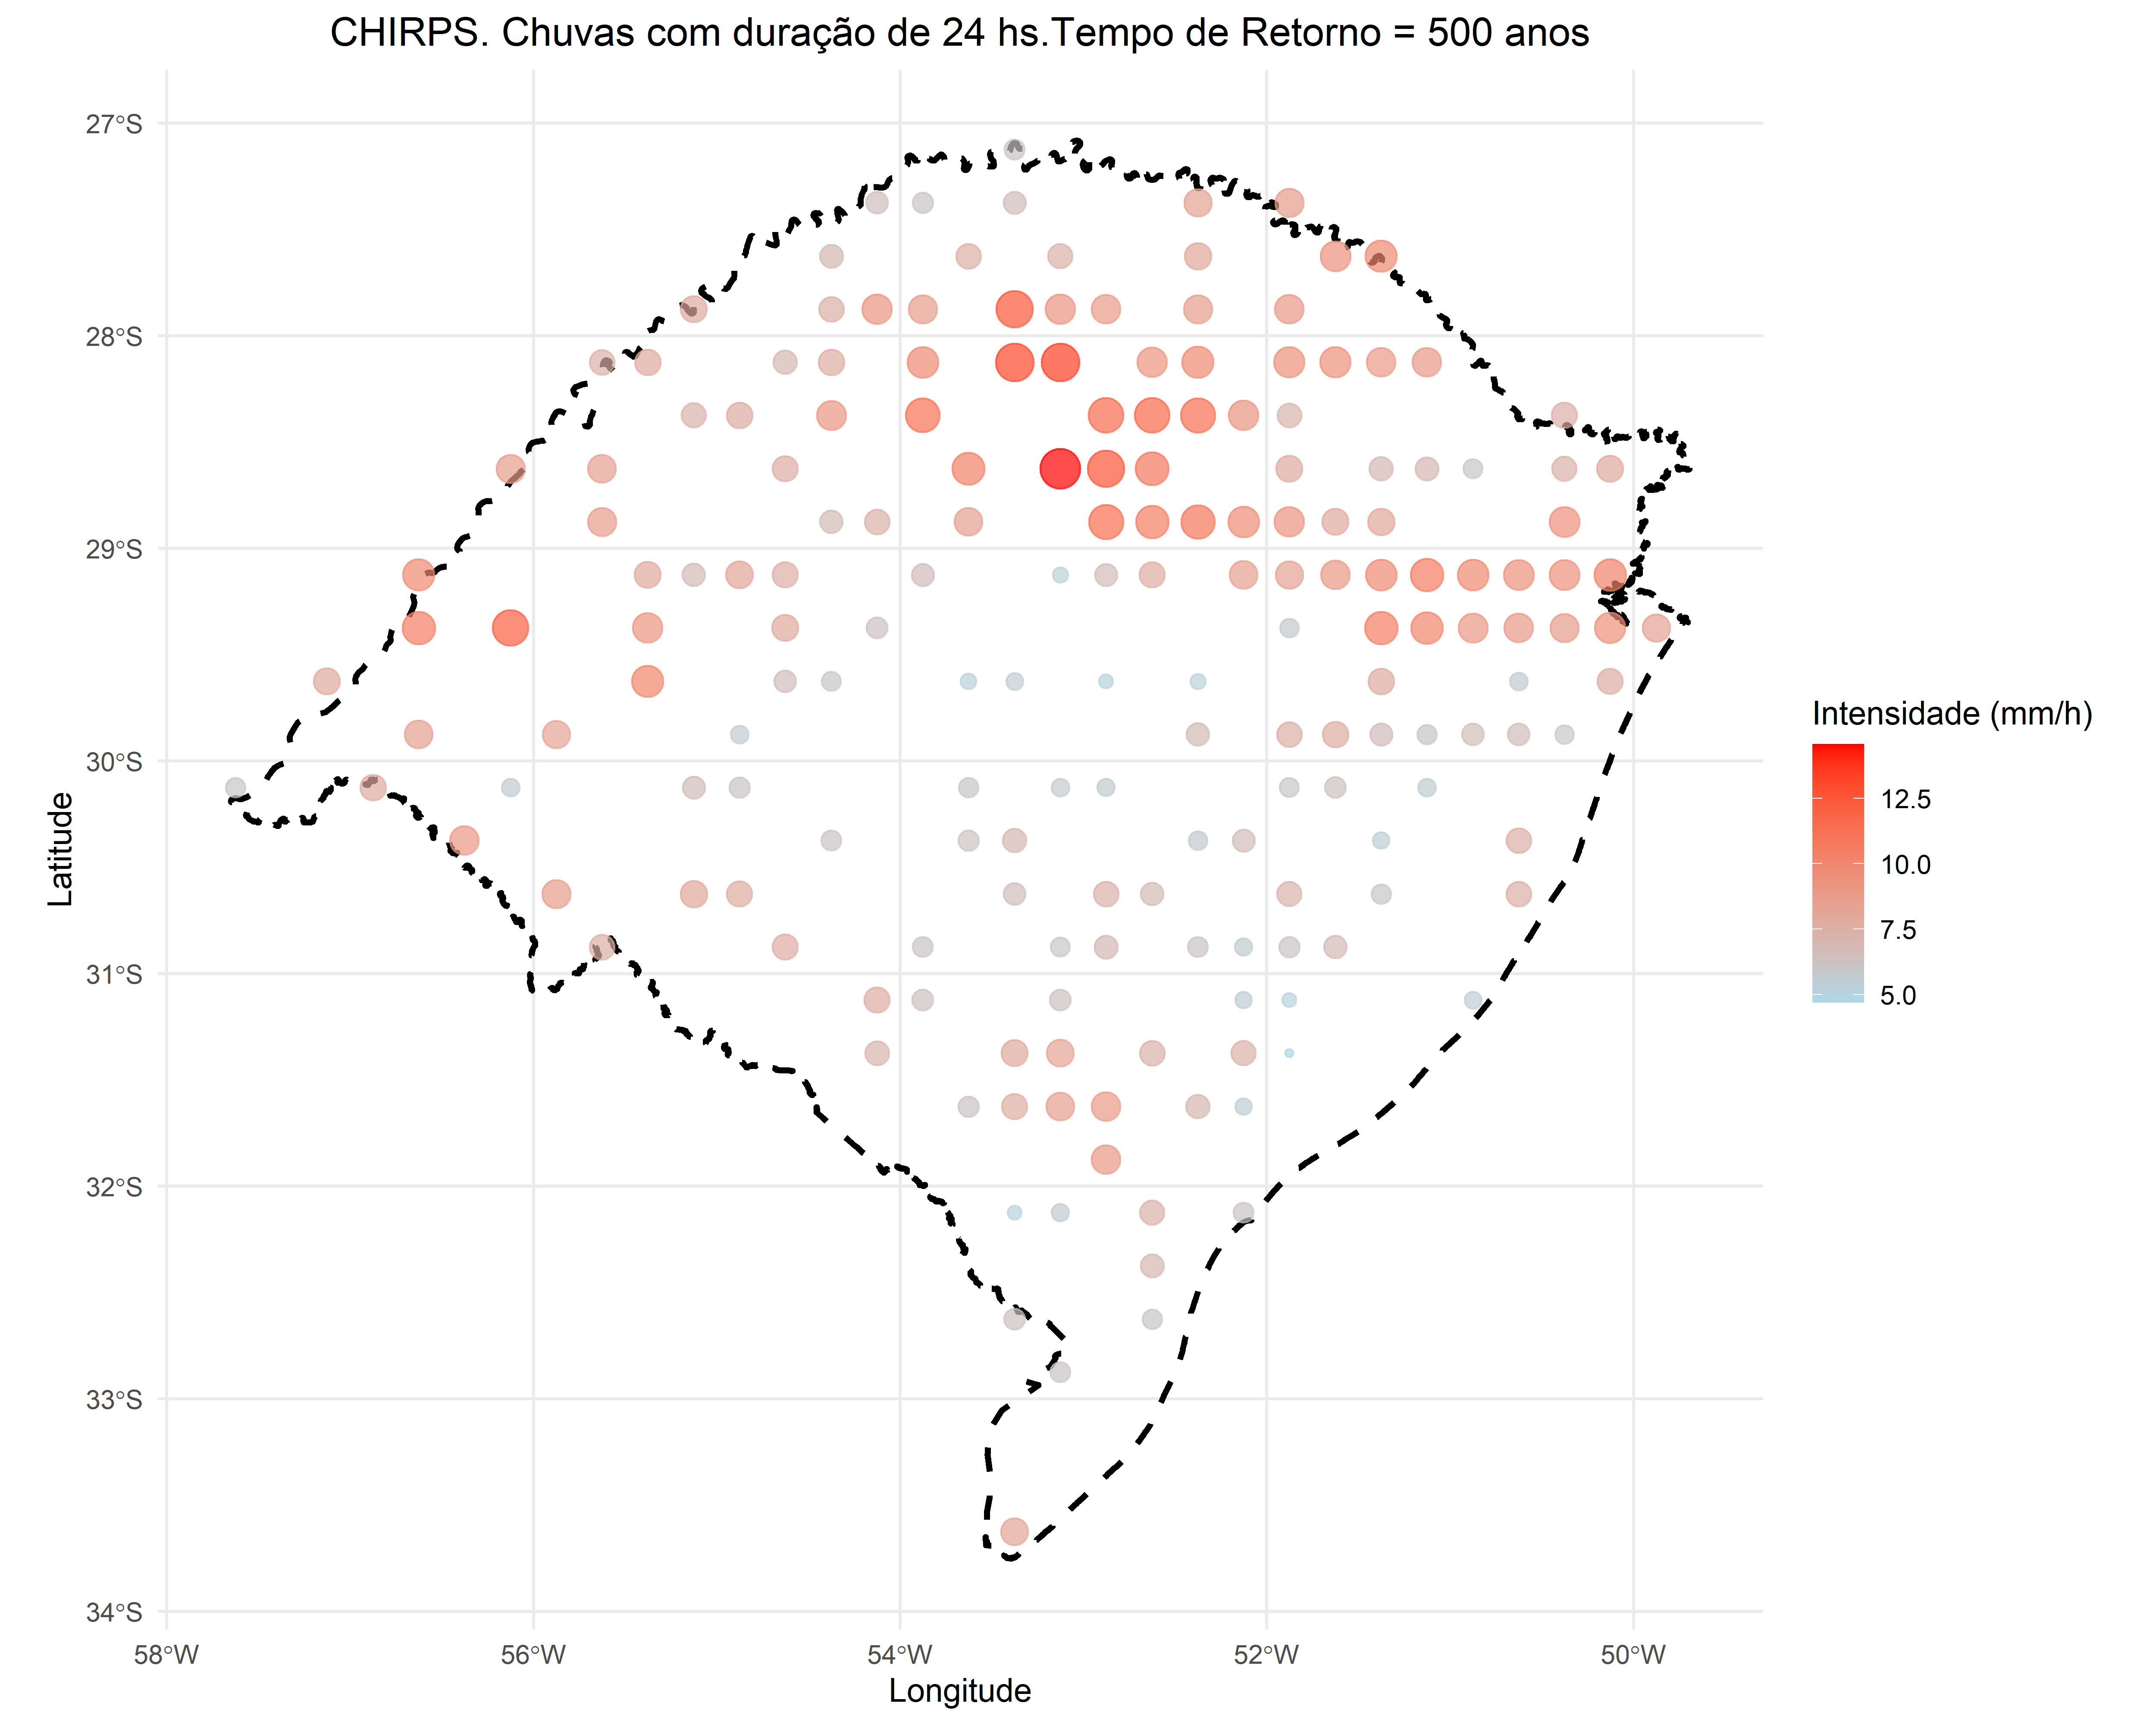
\includegraphics{Figuras/Figura7c.png}

}

\subcaption{\label{fig-Figura7c}Base de dados CHIRPS}

\end{minipage}%

\caption{\label{fig-Figura7}Magnitude da intensidade da precipitação com
duração de 24 horas para o tempo de retorno de 500 anos considerando a
base de dados HDIRO (a); XAVIER (b) e CHIRPS (c). O tamanho dos circulos
azuis indica a magnitude da intensidade das chuvas.}

\end{figure}%

\subsection{Avaliação da ABE}\label{avaliauxe7uxe3o-da-abe}

Conforme anteriormente descrito na seção de Métodos, a ABE buscou, a
partir de método de interpolação, espacializar o padrão das chuvas de
intensidade de 24 horas advindos da base HIDRO para uma resolução em
grade correspondente àquelas das bases XAVIER e CHIRPS. Na sequência,
esses padrões foram comparados com aqueles supostamente correspondentes,
oriundos diretamente de ambas as bases. Contudo, tal como descrito na
metodologia, inicialmente, foi realizada uma análise de sensibilidade
para avaliar o valor ótimo do expoente do polinômio de interpolação para
o método IDW, para cada tempo de retorno estudado, por meio da técnica
LOOCV. Na sequência, a interpolação por IDW obtida a partir da
otimização do parâmetro \(p\) foi confrontada com a espacialização por
krigagem. Só então, após definida a melhor técnica de espacialização
para este caso, realizou-se a comparação dos padrões de chuvas de 24
horas entre as diferentes bases (HIDRO, XAVIER E CHIRPS).

\subsubsection{\texorpdfstring{Otimização do parâmetro \(p\) para o
método
IDW}{Otimização do parâmetro p para o método IDW}}\label{otimizauxe7uxe3o-do-paruxe2metro-p-para-o-muxe9todo-idw}

A Figure~\ref{fig-Figura8} apresenta o resultado da análise de
sensibilidade obtida a partir da técnica LOOCV, exclusivamente, para a
métrica \(RMSE\), considerando os graus de expoente para o parâmetro
\(p\) e os diferentes tempos de retorno avaliados. No eixo vertical
apresenta-se o valor da métrica e no eixo horizontal os valores do
parâmetro \(p\). Os resultados evidenciam que o valor da métrica tende a
aumentar a medida que o tempo de retorno aumenta, independente do valor
do parâmetro \(p\). Ou seja, há um decréscimo da qualidade de
representatividade do modelo para maiores tempos de retorno. O aumento
dos níveis de incerteza para chuvas de maior recorrência pode estar
associado com este comportamento. Outro aspecto visível, consiste no
comportamento padrão das curvas que indicam a existência de um valor
ótimo (menor valor da métrica) para cada tempo de retorno.

\begin{figure}

\begin{minipage}{\linewidth}

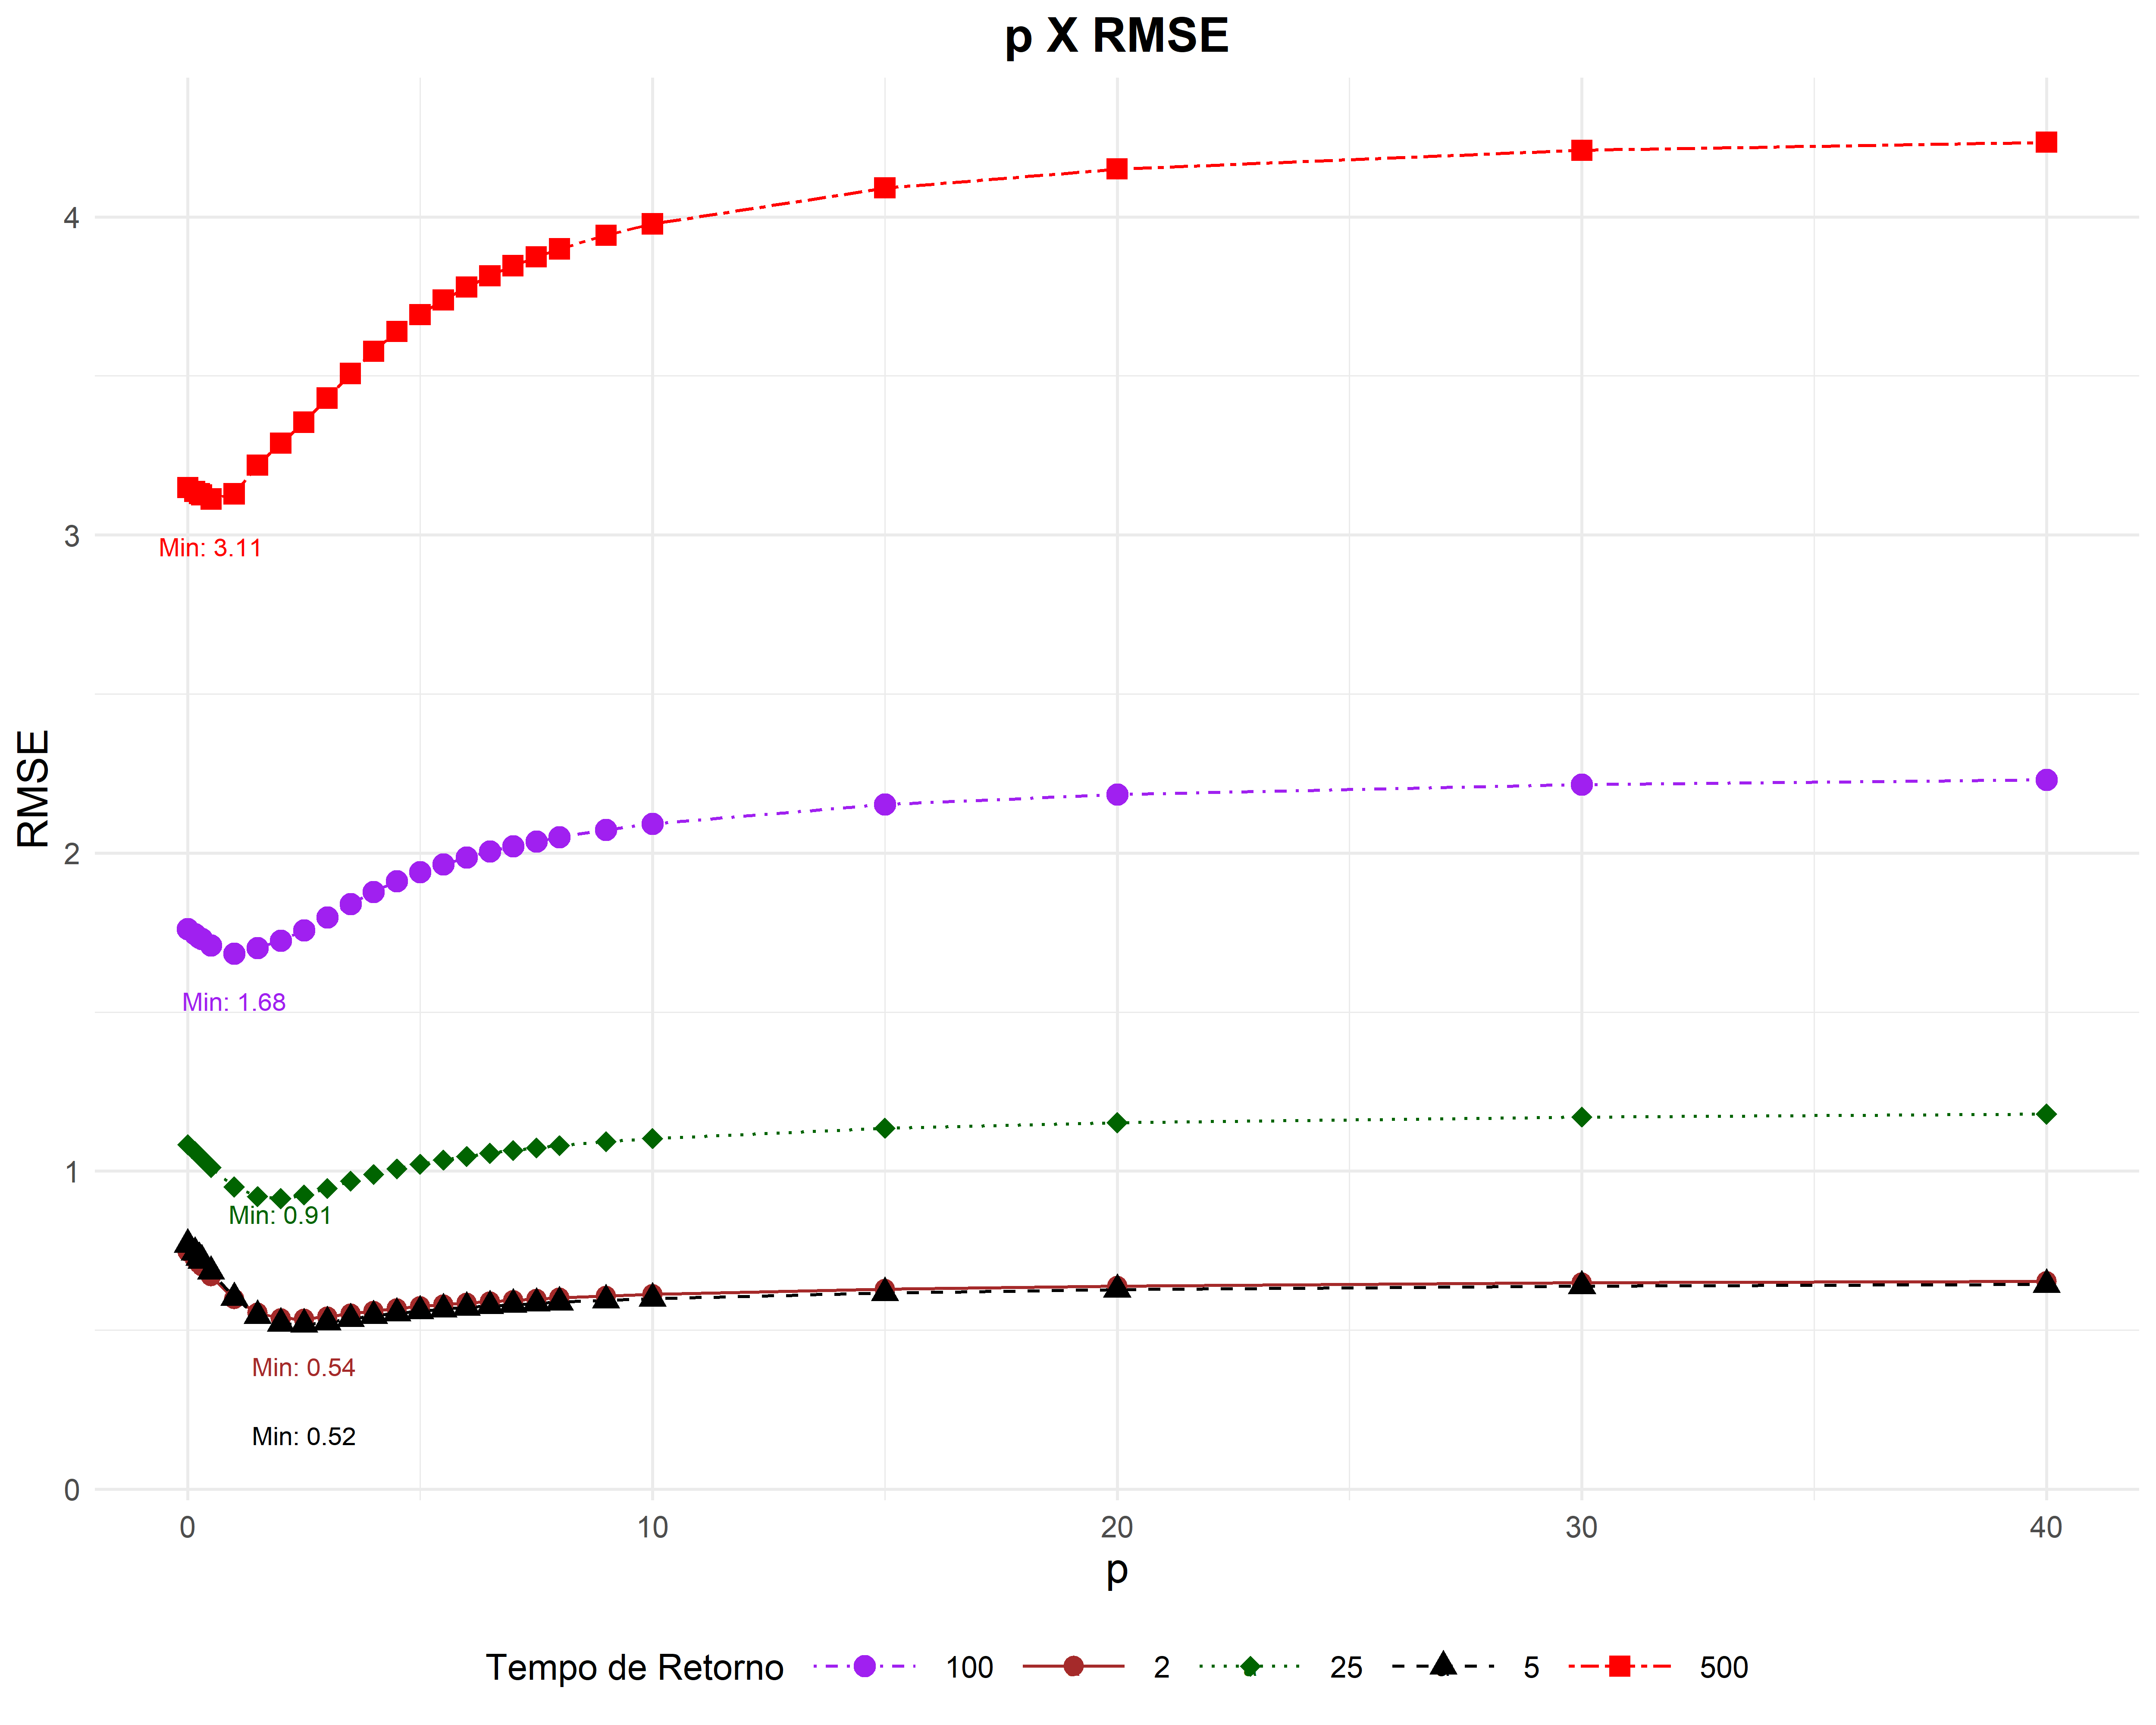
\includegraphics{Figuras/Figura8.png}

\end{minipage}%

\caption{\label{fig-Figura8}Valores da métrica RMSE em função do valor
do parâmetro \(p\) que consiste no expoente do termo correspondente ao
inverso da distância no método IDW. Cada curva representa o
comportamento para um tempo de retorno diferente. Os menores valores da
métrica são indicados para cada curva correspondente}

\end{figure}%

A Figure~\ref{fig-Figura9} mostra os mesmos valores obtidos para métrica
RMSE, porém, confrontados com o percentual de diferença entre a reta 1:1
(predição perfeita) e o coeficiente angular da reta de regressão, entre
os valores preditos e observados (\%\(\Delta\)S). São verificadas as
frentes de Pareto para essas duas métricas, em que os valores mais
próximos da origem indicam os melhores valores para \(p\), que estão
destacados em cada curva. Esses resultados também mostram que que todos
os coeficientes angulares resultaram em valores negativos confirmando a
tendência de que o modelo sempre tende a subestimar os valores preditos
(viés de subestimativa dos valores).

\begin{figure}

\begin{minipage}{\linewidth}

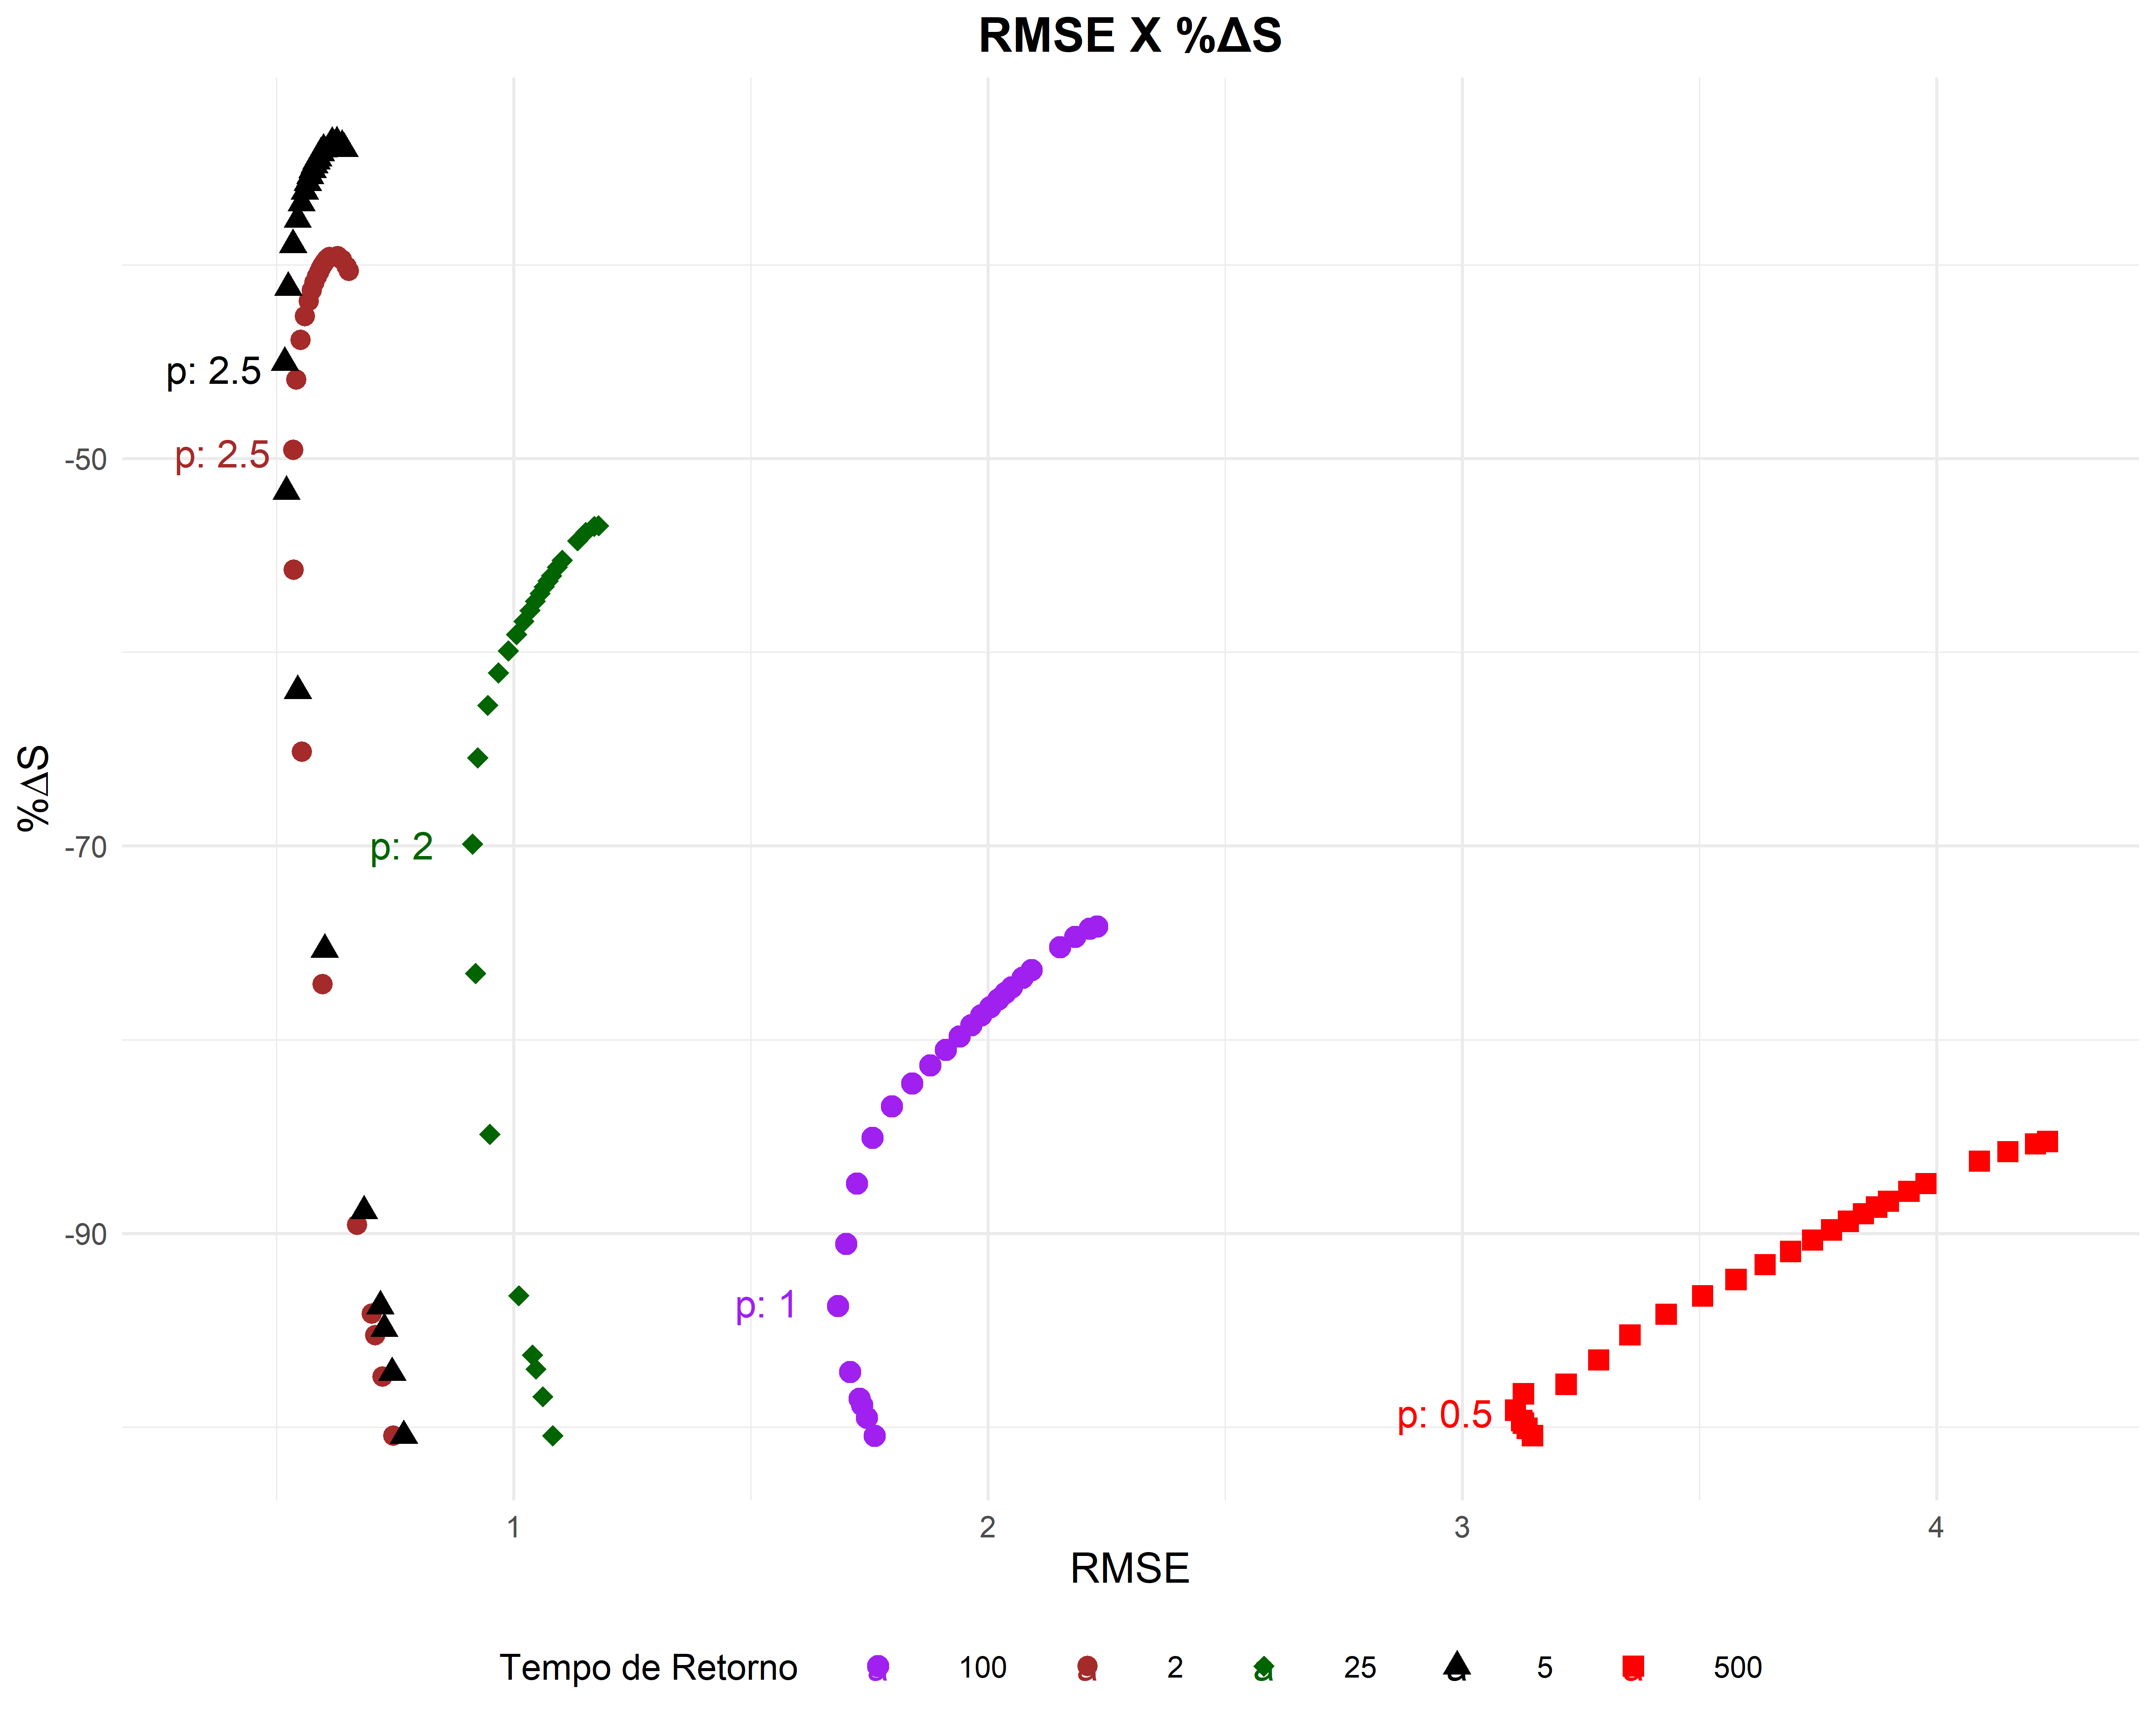
\includegraphics{Figuras/Figura9.png}

\end{minipage}%

\caption{\label{fig-Figura9}Frentes de pareto para os valores de RMSE e
\%\(\Delta\)S. Cada curva representa o comportamento para um tempo de
retorno diferente. Os valores ótimos do parâmetro \(p\) são destacados
em cada curva.}

\end{figure}%

A Table~\ref{tbl-Tab6} apresenta um resumo dos resultados para os
valores ótimos do parâmetro \(p\) em função do tempo de retorno.
Verifica-se que quanto maior o tempo de retorno menor o valor do
parâmetro \(p\). Valores menores de \(p\) indicam que a influência da
distância é menor (ou seja, as estações distantes têm uma influência
maior). Se o tempo de retorno maior está associado a um menor valor de
\(p\), isso sugere que, em eventos de alta intensidade, a influência das
estações mais próximas é relativamente menor em comparação com eventos
de baixa intensidade. Dessa forma, a alta intensidade de precipitação
pode ter uma correlação espacial diferente comparada com eventos de
menor intensidade. Uma possível explicação é que em áreas de maior
intensidade de chuva (tempos de retorno maiores), pode haver uma
distribuição mais homogênea da precipitação em comparação com áreas de
menor intensidade. Se a chuva é mais intensa e distribuída uniformemente
em áreas maiores, o impacto relativo das distâncias nas estimativas pode
ser menor, resultando em um menor valor de \(p\) (o que indica um menor
peso para estações distantes). Contudo, esse fenômeno pode ser complexo
e depender de diversos outros fatores interrelacionados que não foram
objetos desta análise e precisam ser melhor investigados.

\begin{longtable}[]{@{}ll@{}}
\caption{Valores ótimos para o parâmetro \(p\) do método IDW em função
do tempo de retorno.}\label{tbl-Tab6}\tabularnewline
\toprule\noalign{}
Tempo de Retorno (anos) & Parâmetro Ótimo \(p\) \\
\midrule\noalign{}
\endfirsthead
\toprule\noalign{}
Tempo de Retorno (anos) & Parâmetro Ótimo \(p\) \\
\midrule\noalign{}
\endhead
\bottomrule\noalign{}
\endlastfoot
2 & 2,5 \\
5 & 2,5 \\
25 & 2,0 \\
100 & 1,0 \\
500 & 0,5 \\
\end{longtable}

\subsubsection{Comparação IDW X
Krigagem}\label{comparauxe7uxe3o-idw-x-krigagem}

As Figuras 10 a 14 apresentam os resultados comparativos das
interpolações realizadas por IDW e OK para os diferentes tempos de
retorno testados (2, 5, 25, 100 e 500 anos), respectivamente. Para cada
figura dessa sequência são apresentados os resultados da espacialização
por IDW (a) e OK (b) e os resultados das predições em função dos valores
observados, juntamente com as retas de regressão linear e a reta de
referência 1:1, incluindo as métricas \(RMSE\) e \(MAPE\) para os
modelos IDW (c) e OK (d).

Tal como esperado, o modelo IDW tende a atribuir mais pesos à influência
localizada de cada estação, de tal forma que visualmente os valores
interpolados parecem reproduzir com mais proximidade aqueles observados
na própria estação, quando se compara a escala de cores dos valores
observados nas estações e aqueles interpolados. O modelo OK , por sua
vez, por levar em consideração a variabilidade espacial dos dados além
da distância, distribui de forma mais homogeneizada e suave a
interpolação dos valores. Outro comportamento que pode ser observado
independente da técnica de interpolação é que para maiores valores de
tempos de retorno a performance do modelo diminui.

\begin{figure}

\begin{minipage}{\linewidth}

\centering{

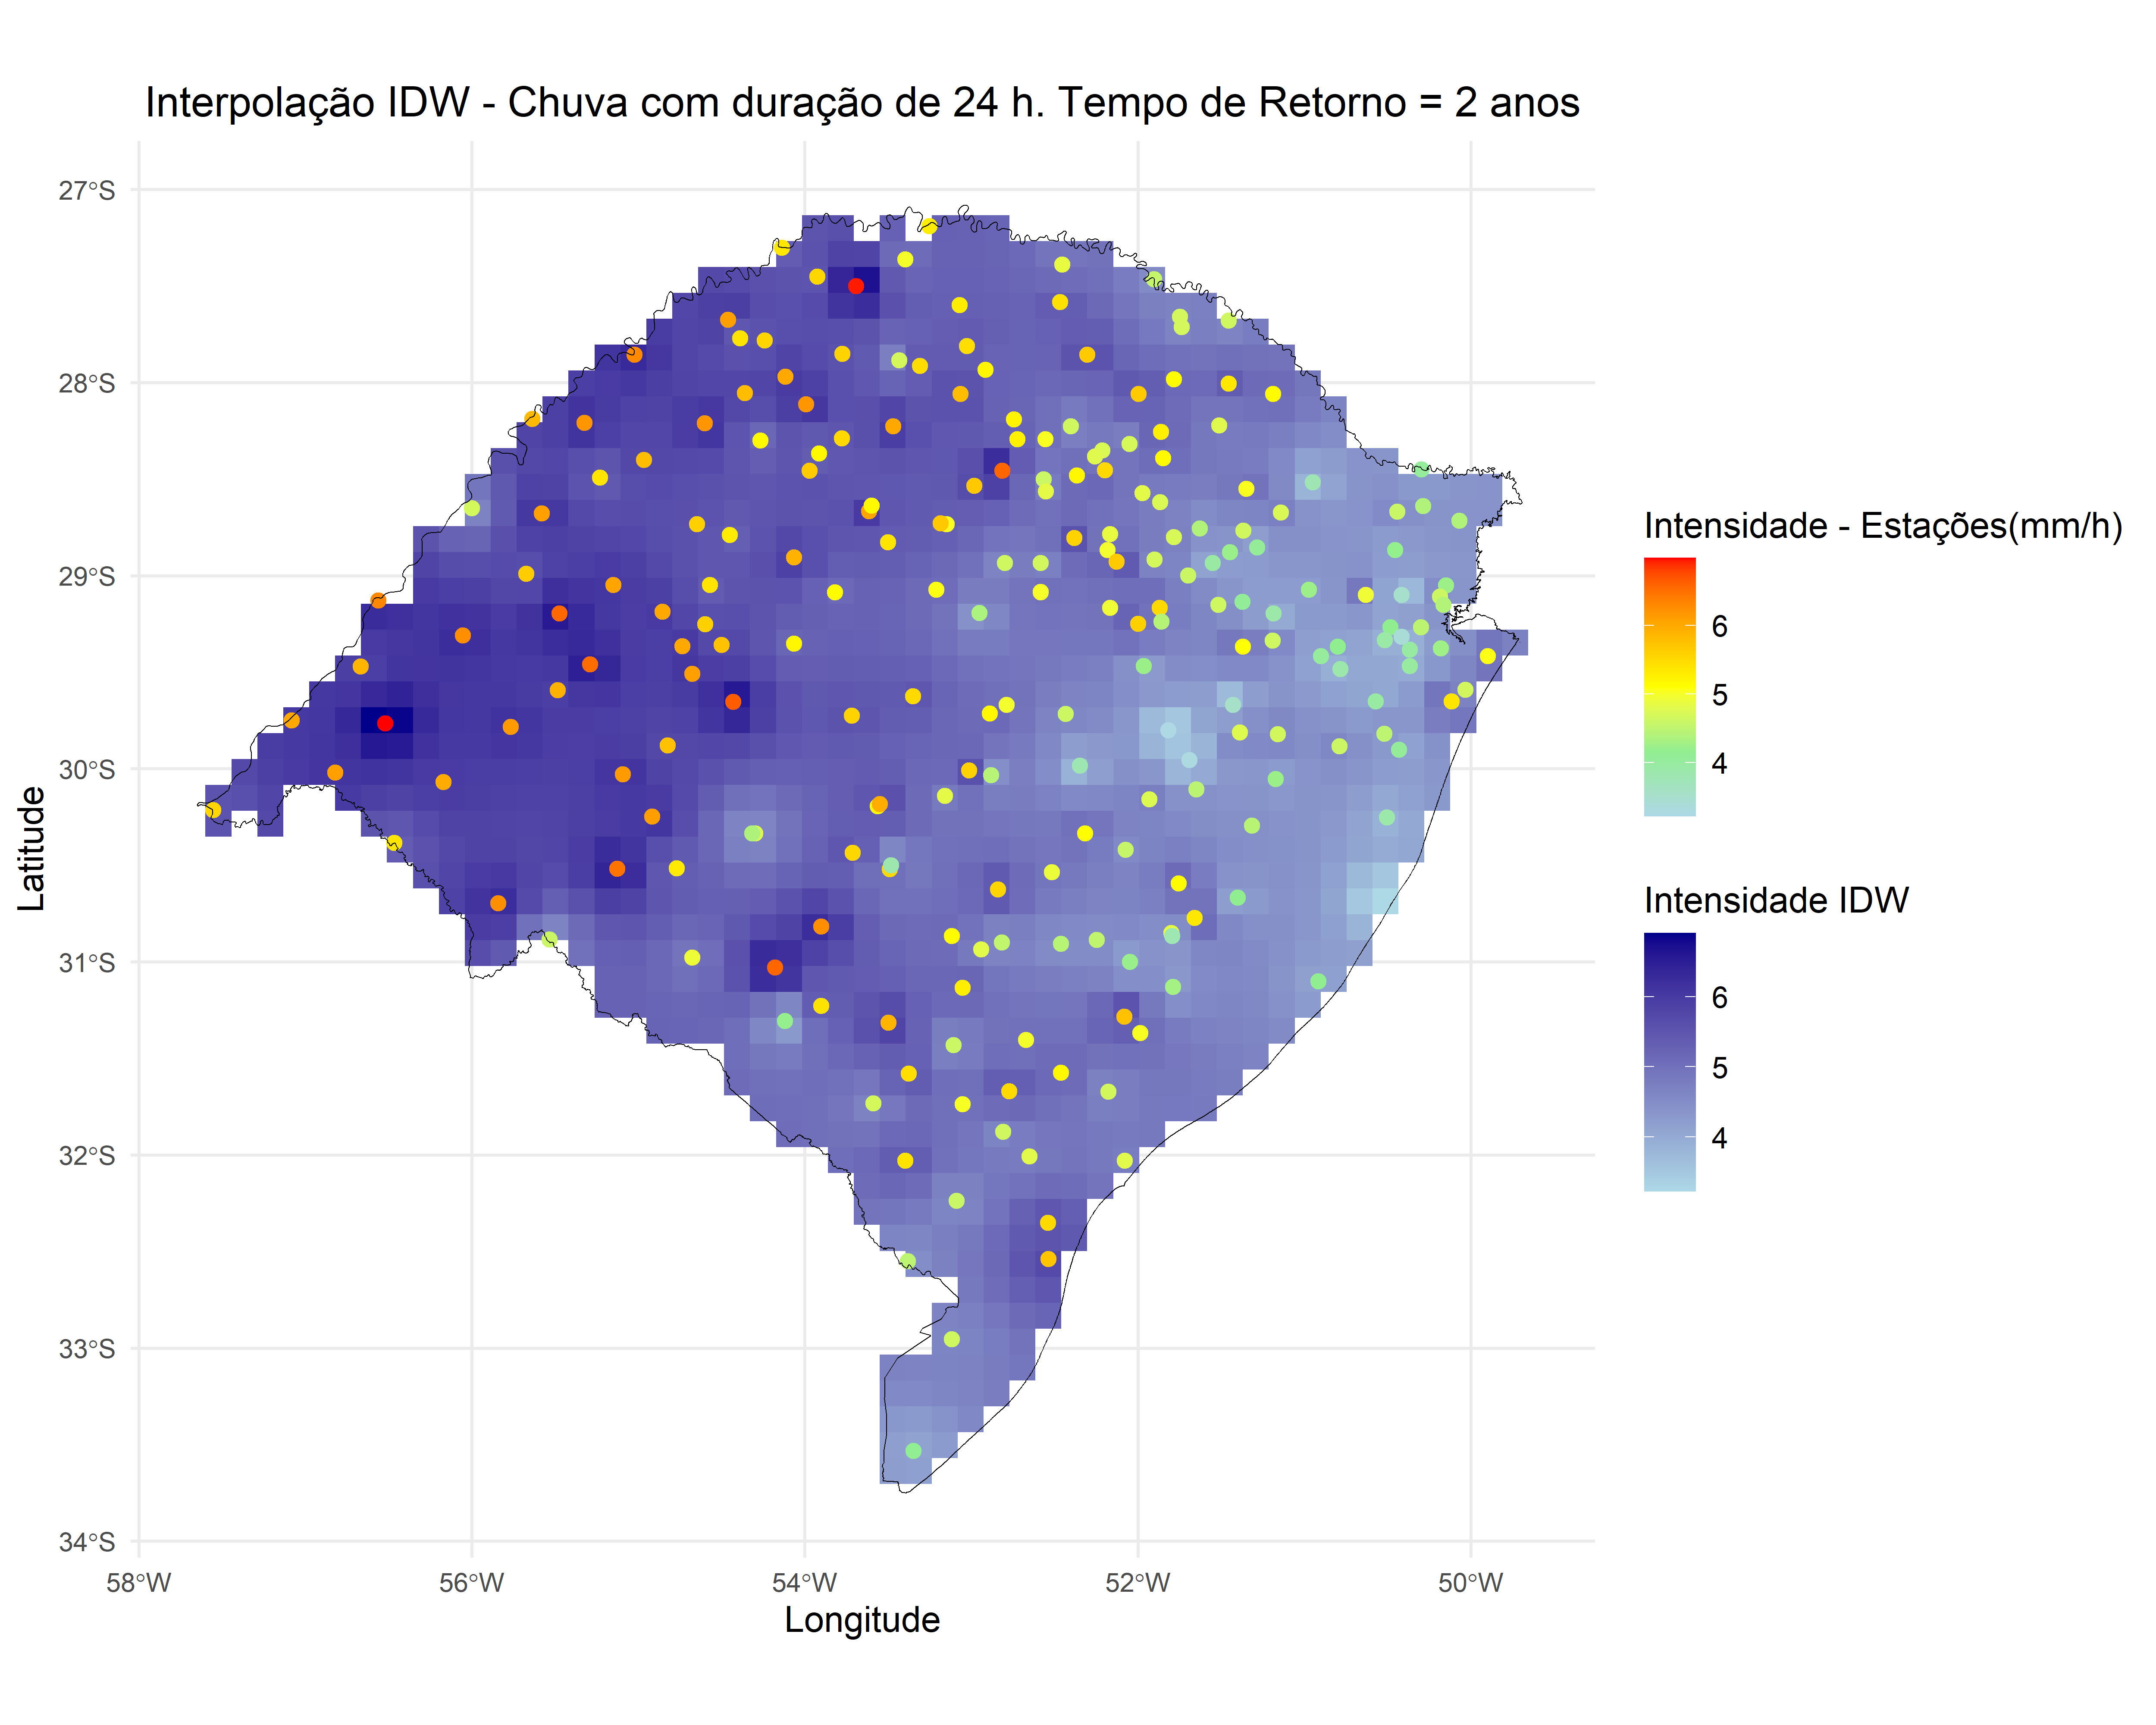
\includegraphics{Figuras/Figura10a.png}

}

\subcaption{\label{fig-Figura10a}Espacialização por IDW (p=2,5). Tempo
de Retorno =2 anos}

\end{minipage}%
\newline
\begin{minipage}{\linewidth}

\centering{

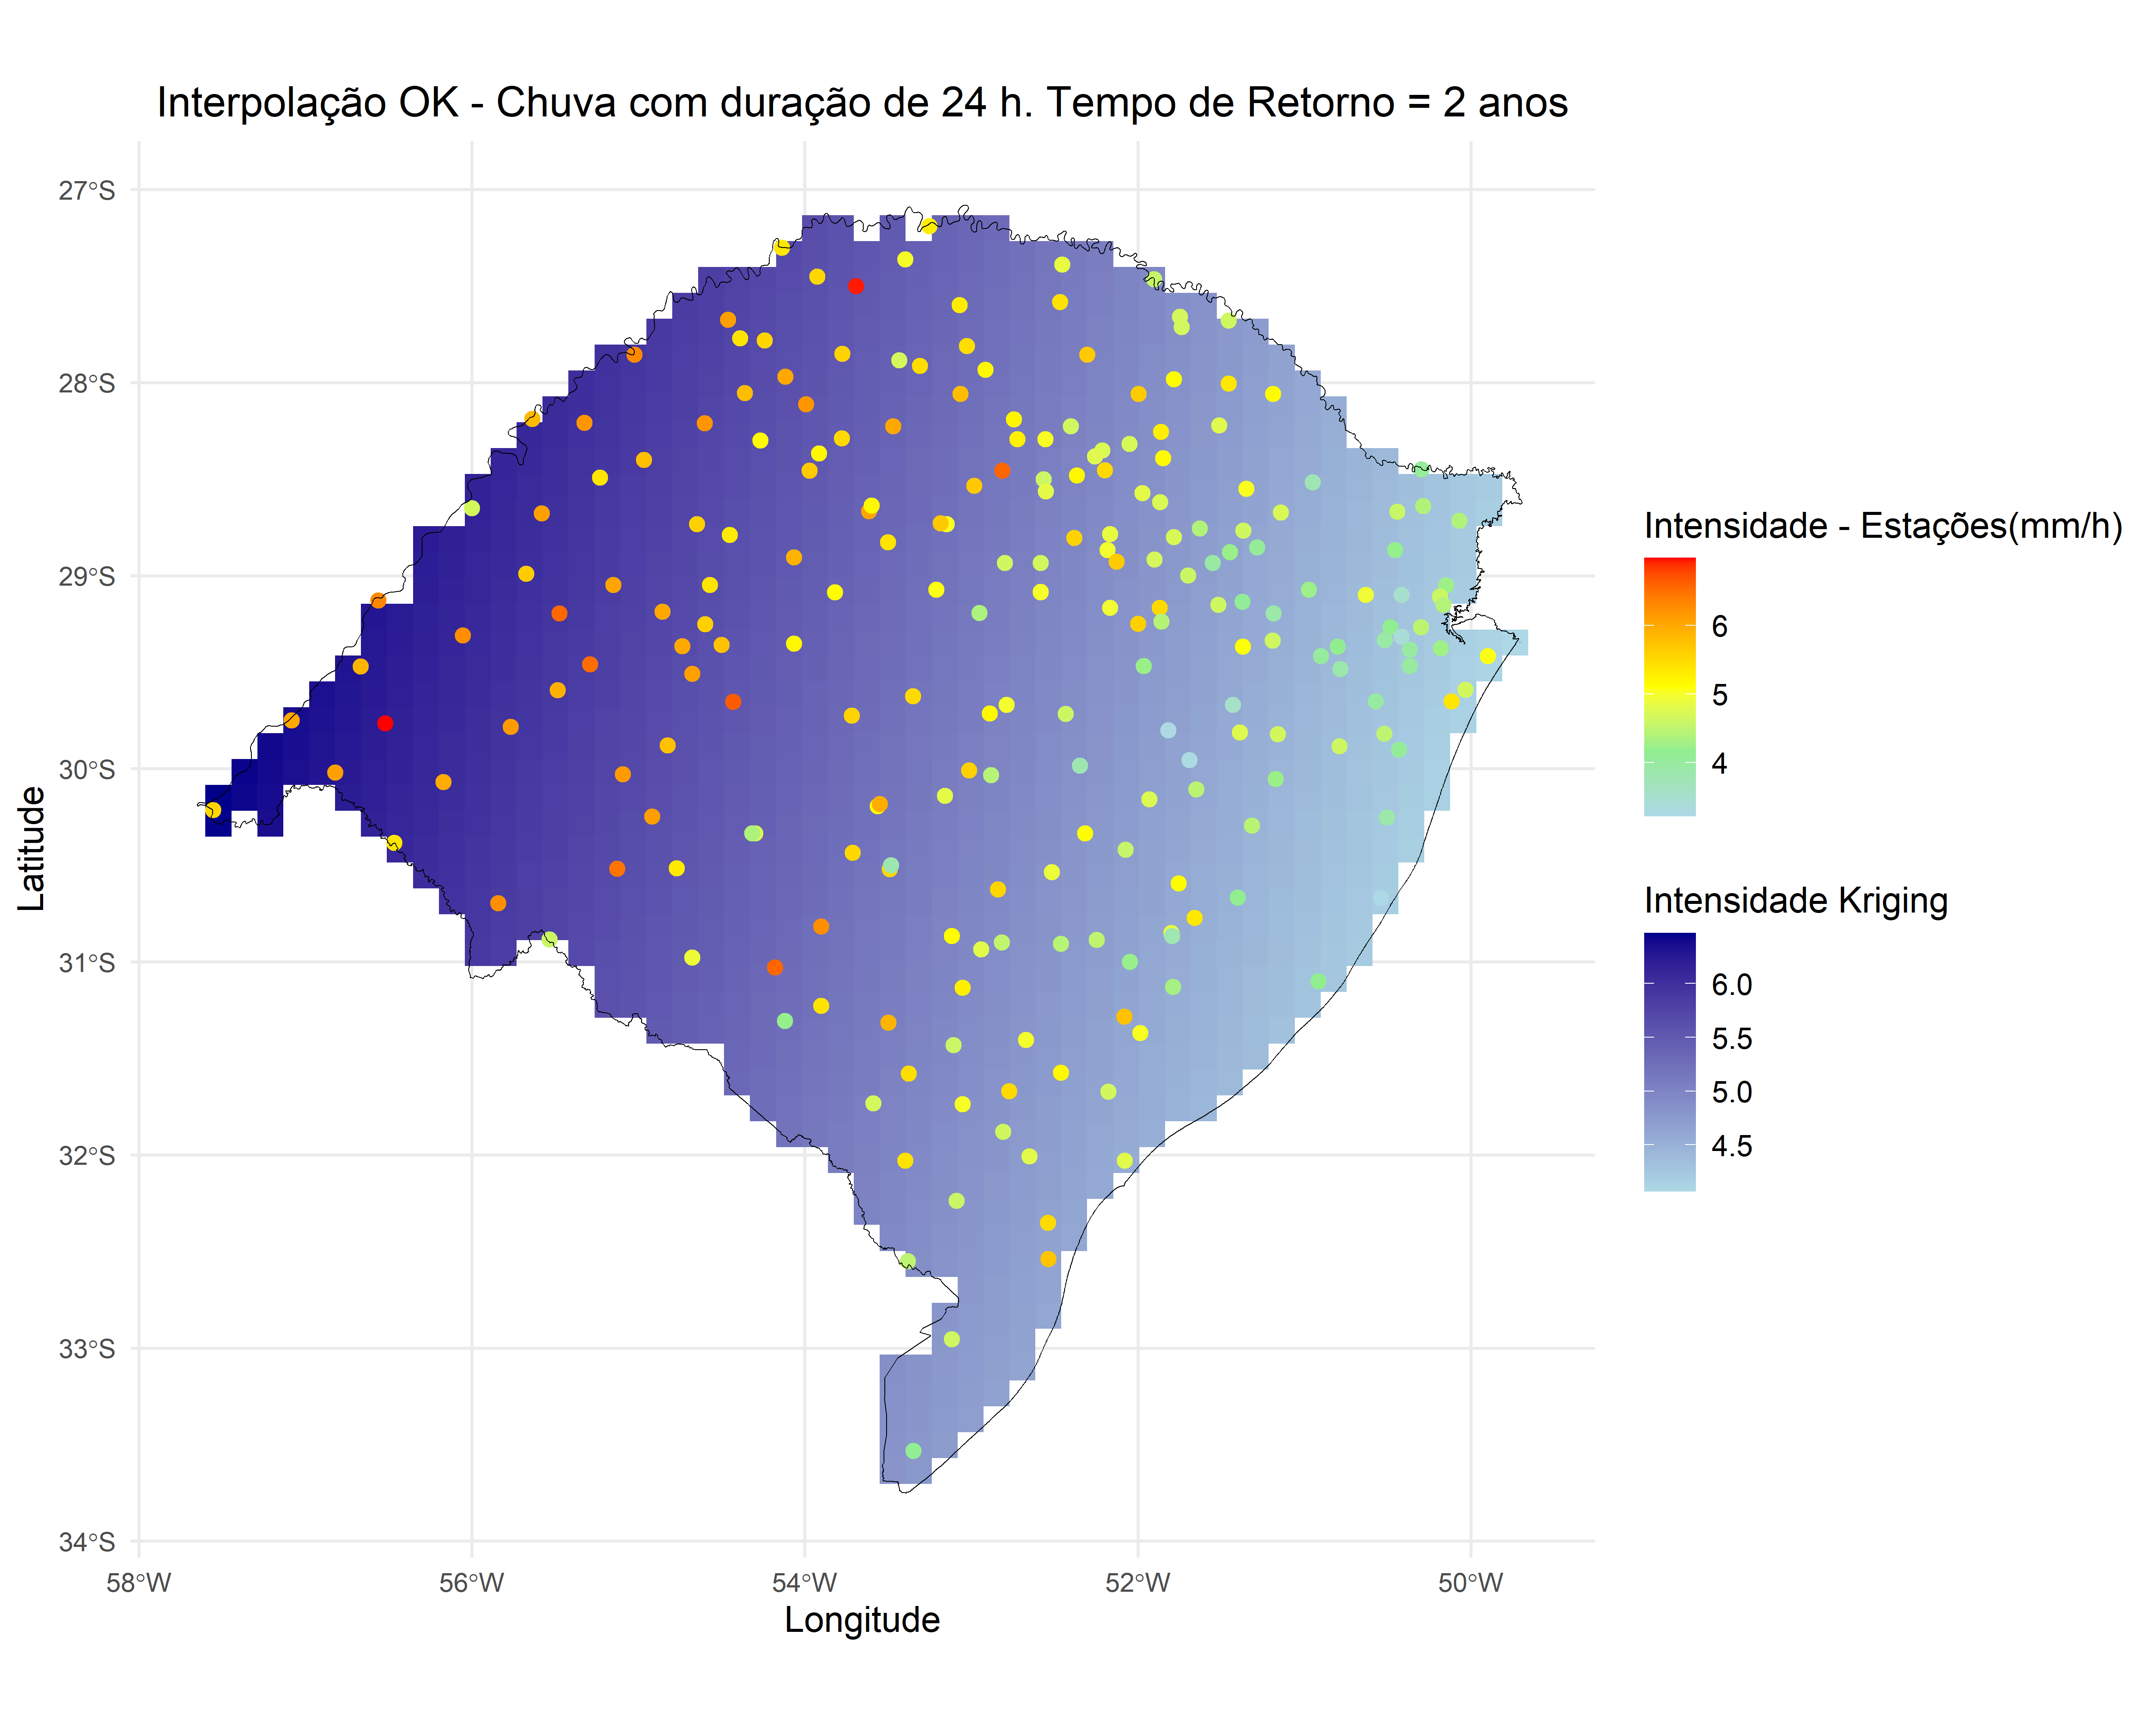
\includegraphics{Figuras/Figura10b.png}

}

\subcaption{\label{fig-Figura10b}Espacialização por OK. Tempo de Retorno
=2 anos}

\end{minipage}%
\newline
\begin{minipage}{\linewidth}
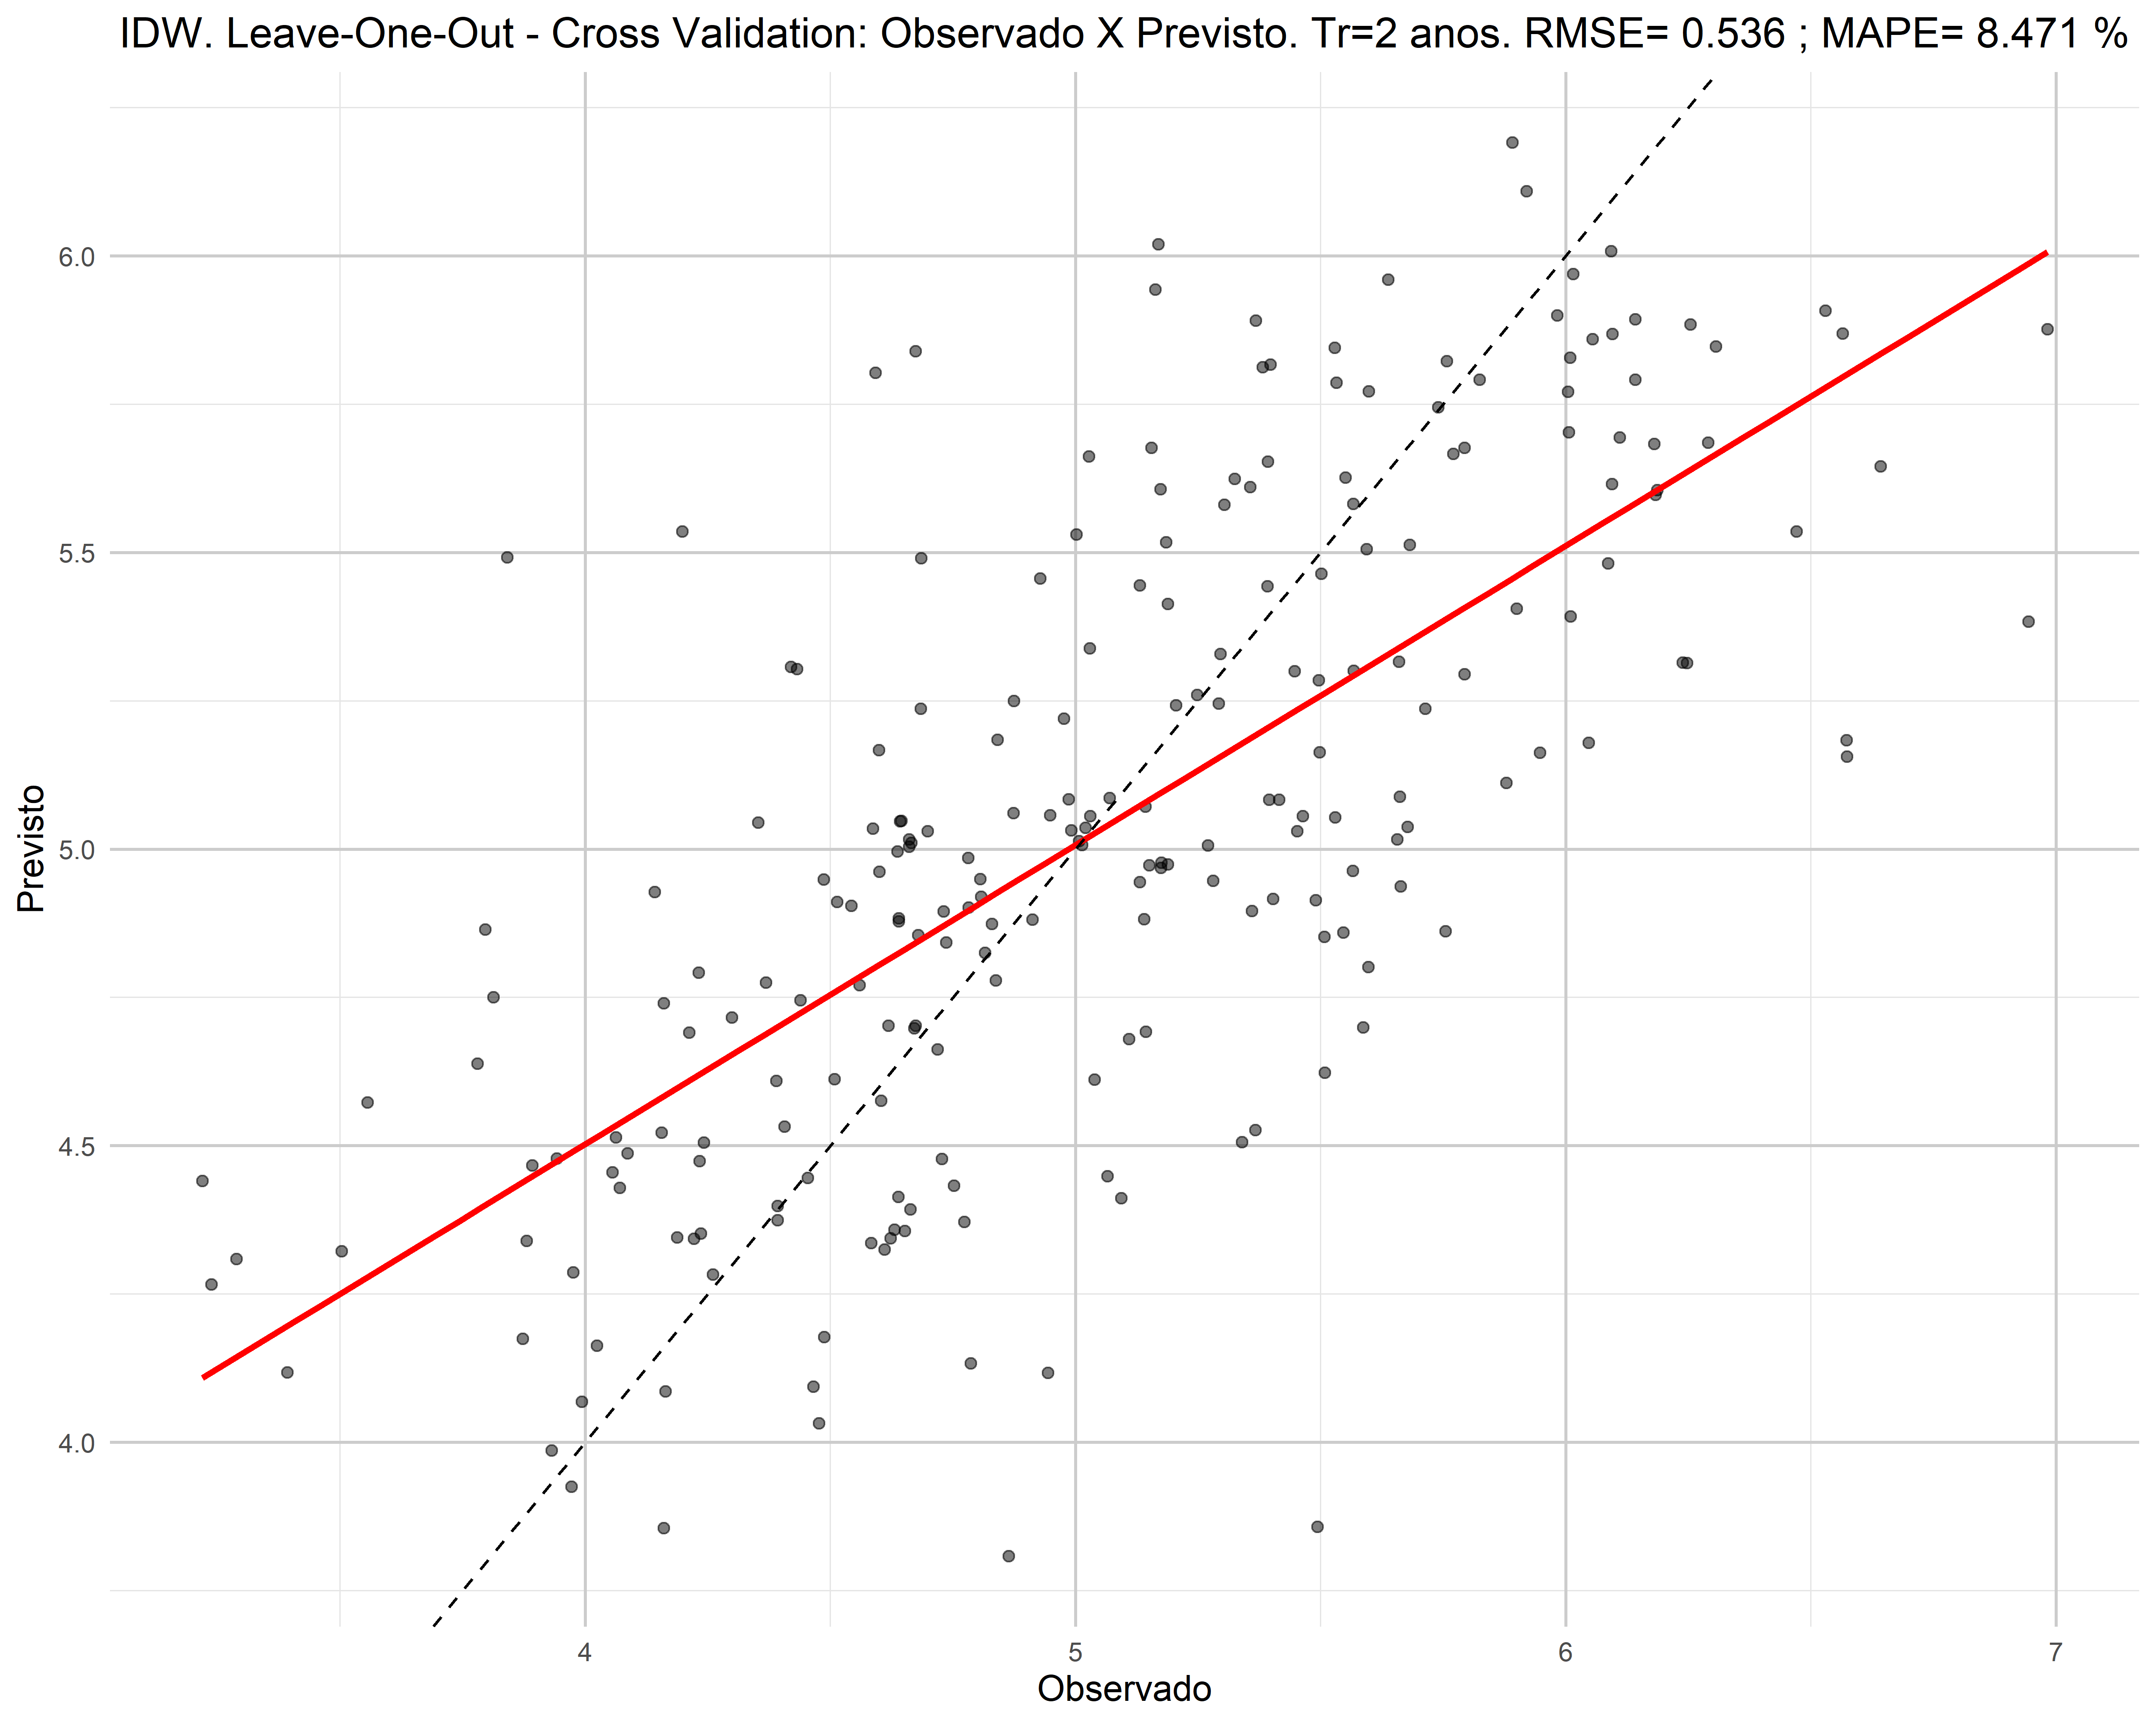
\includegraphics{Figuras/Figura10c.png}
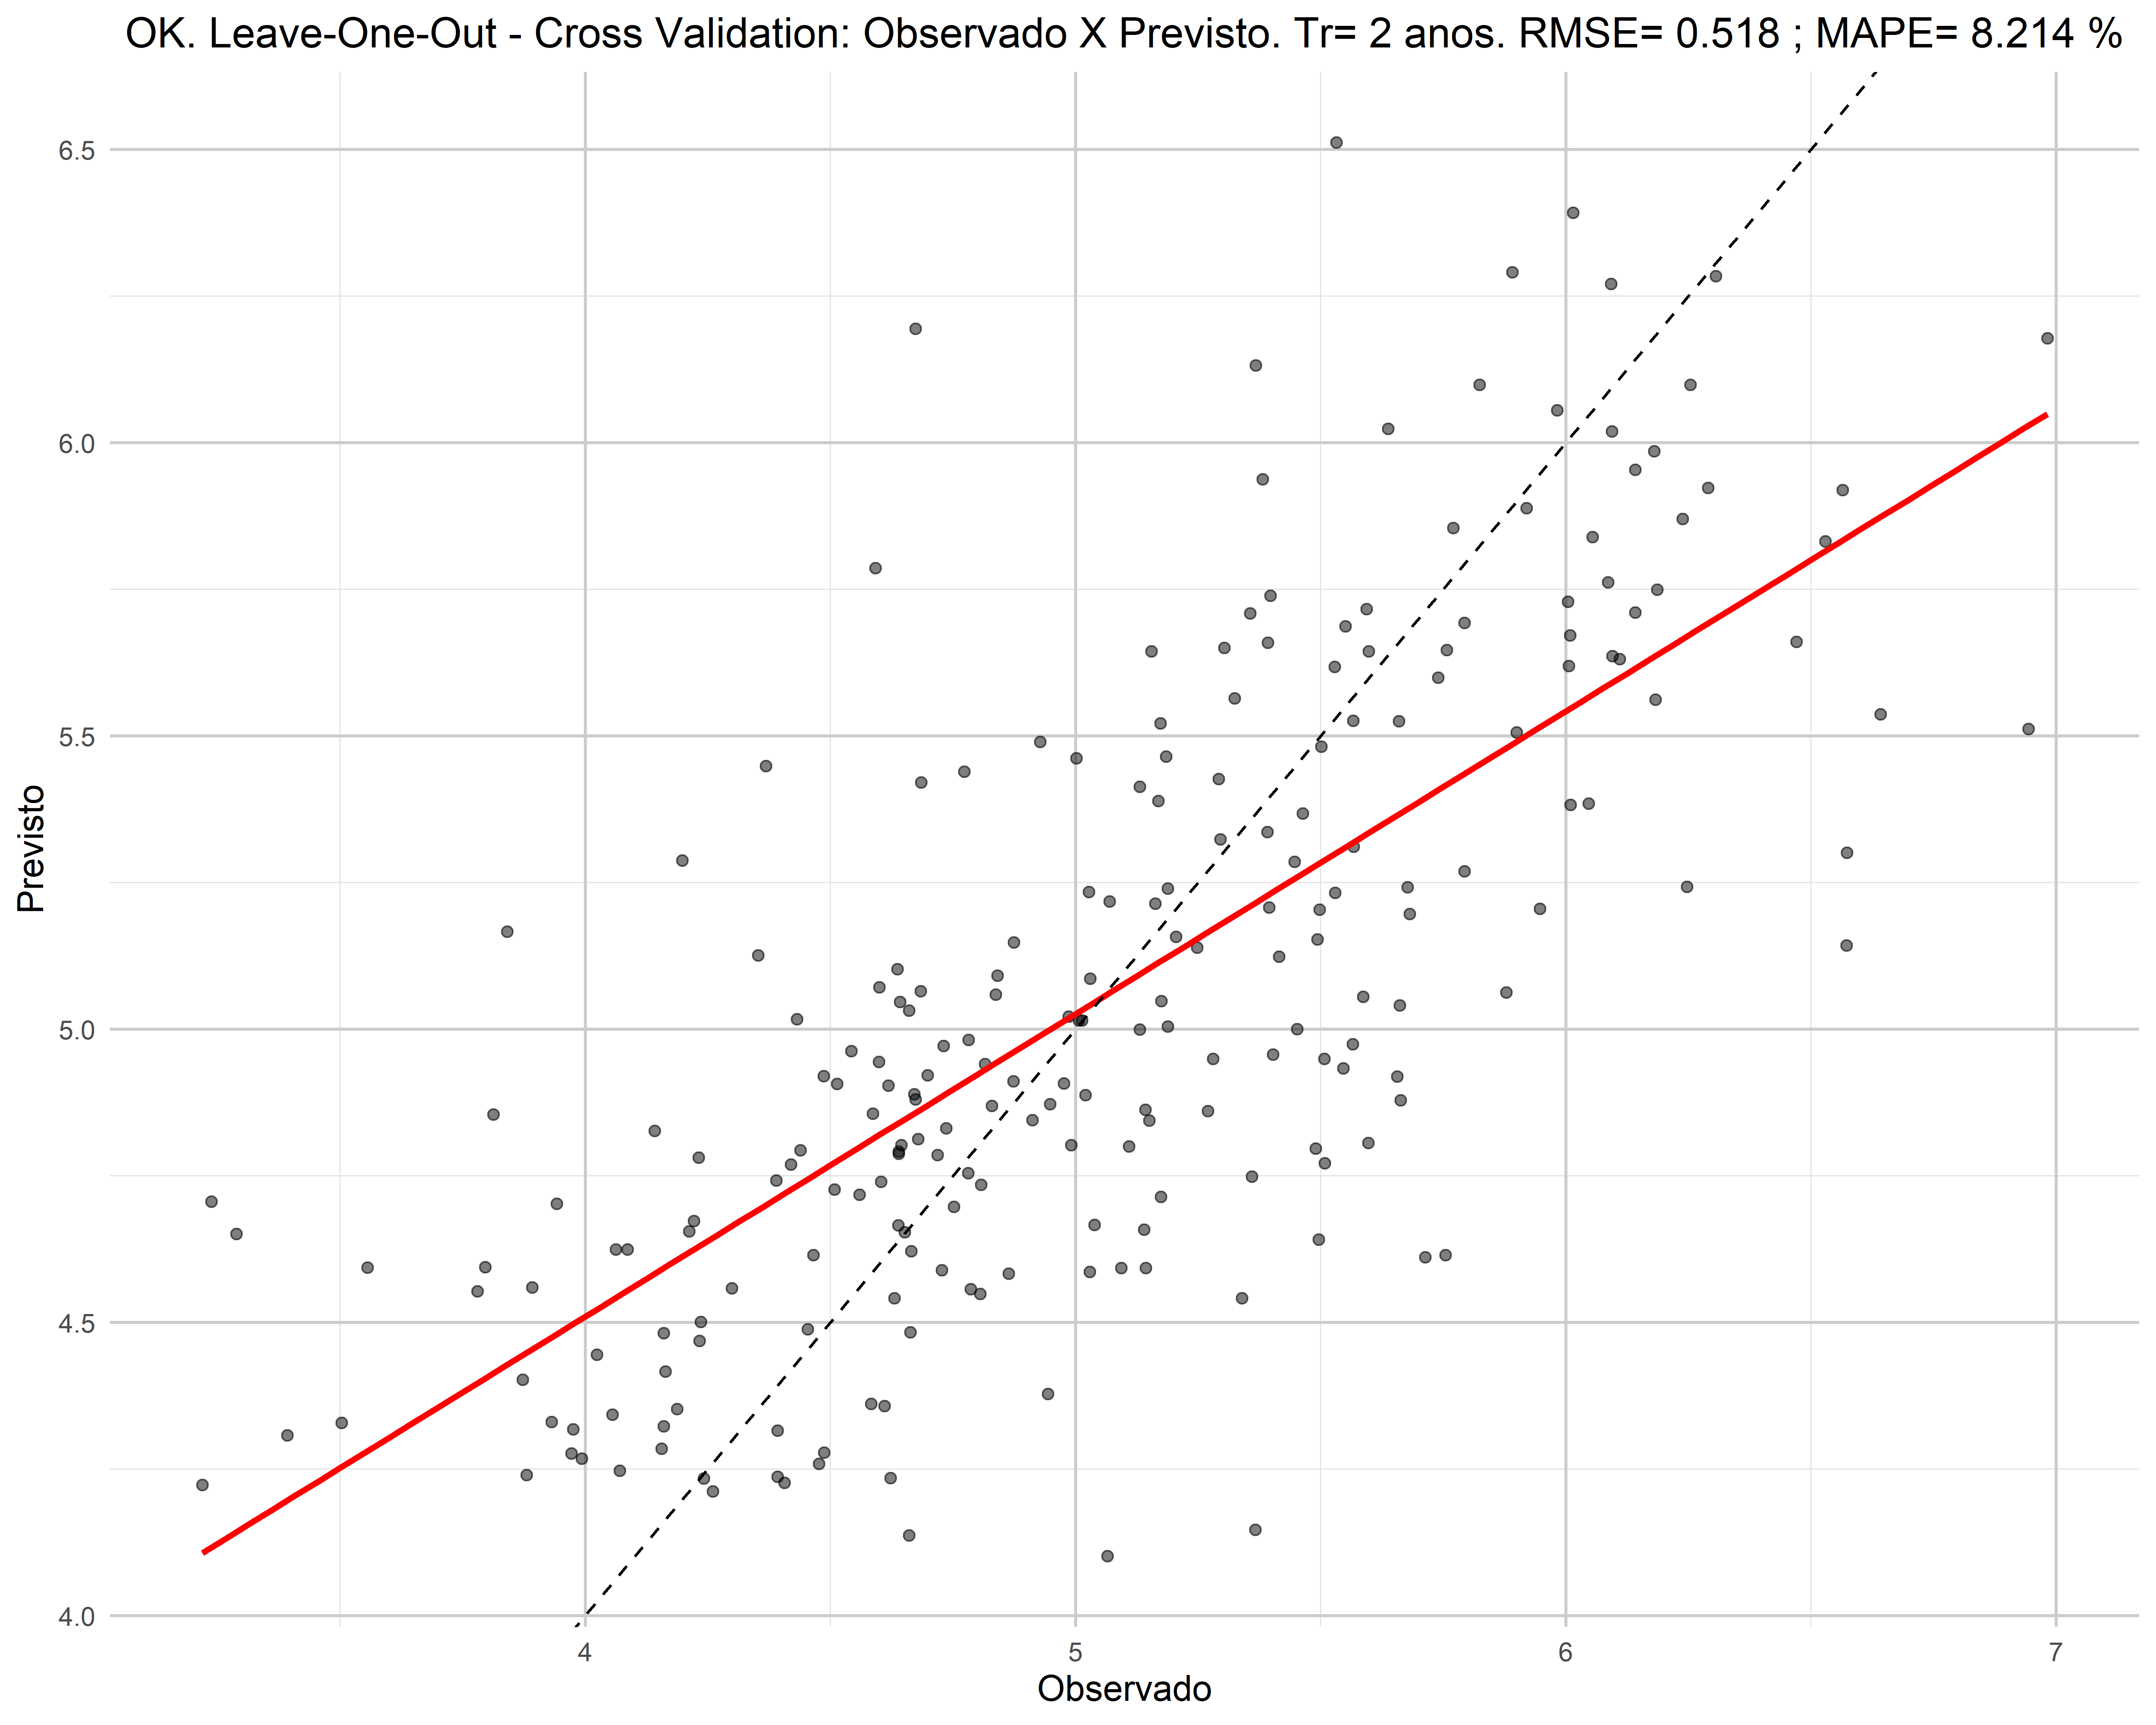
\includegraphics{Figuras/Figura10d.png}\end{minipage}%

\caption{\label{fig-Figura10}Resultados obtidos para intensidade da
chuva de duração de 24 h e tempo de retorno de 2 anos para interpolação
por IDW (a) e por krigagem ordinária, OK (b). Valores preditos em função
dos valores observados e resultados das métricas RMSE e MAPE para
interpolação por IDW (c) e OK (d).}

\end{figure}%

\begin{figure}

\begin{minipage}{\linewidth}

\centering{

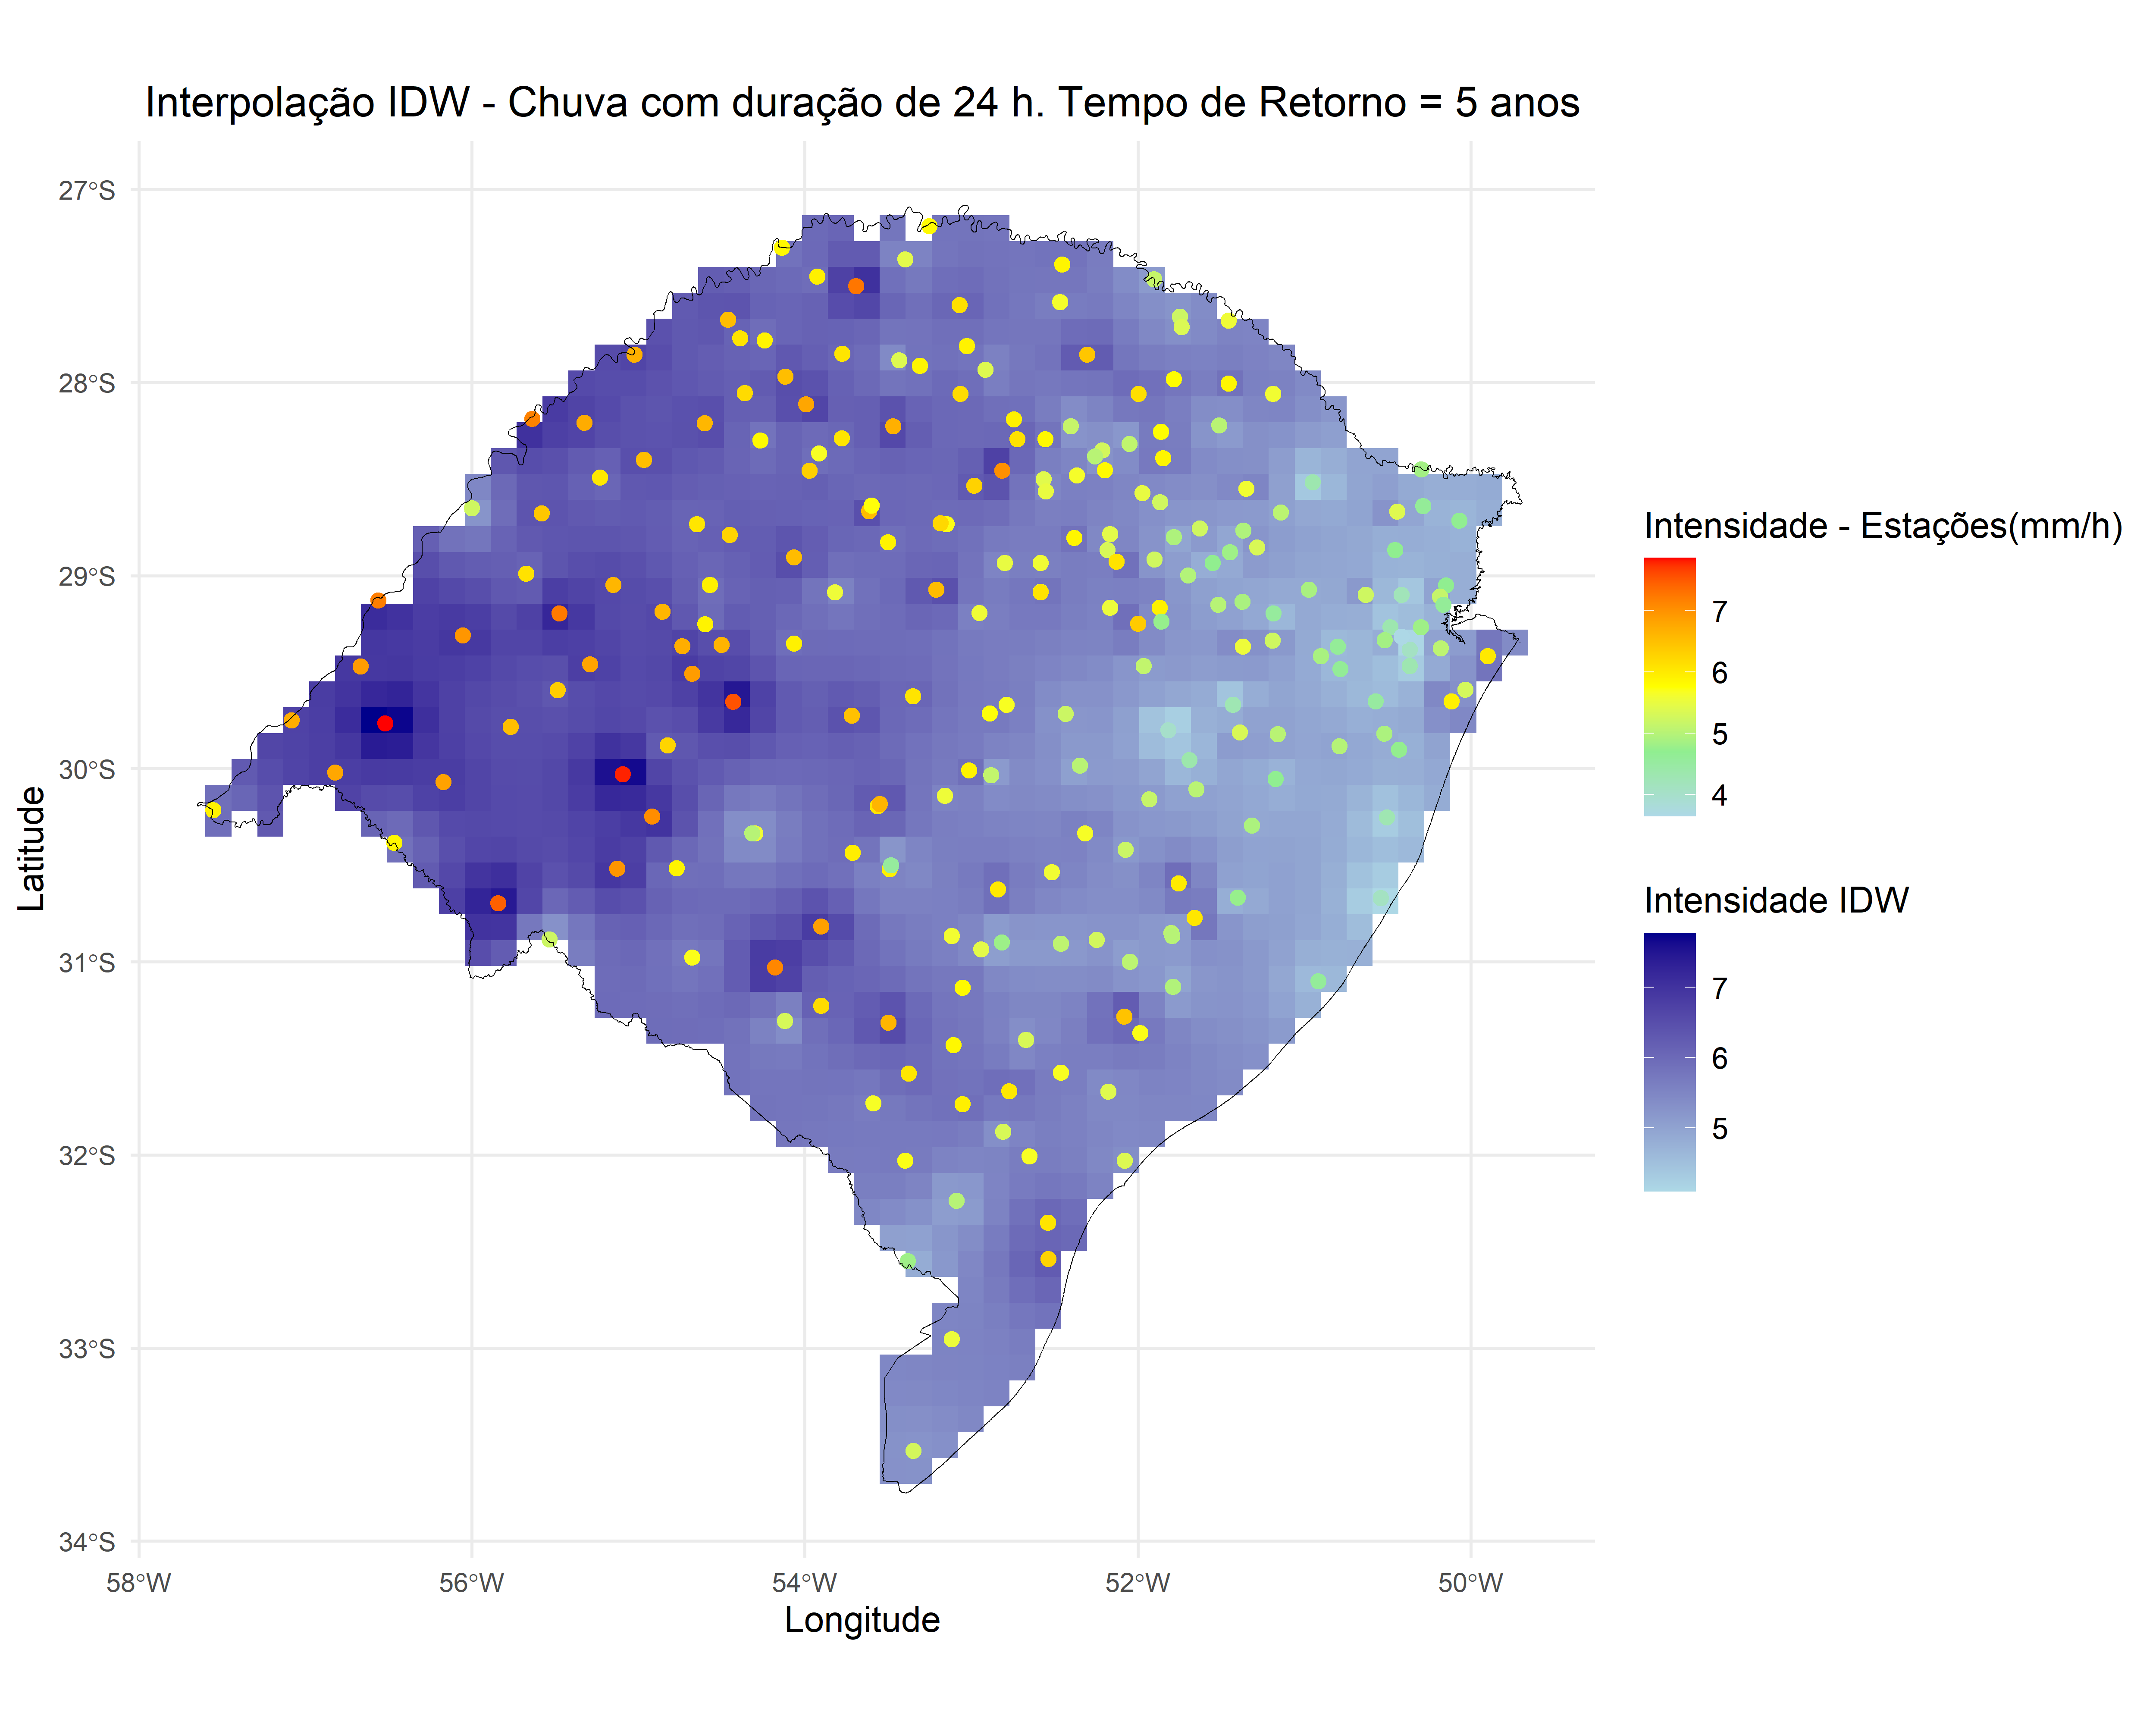
\includegraphics{Figuras/Figura11a.png}

}

\subcaption{\label{fig-Figura11a}Espacialização por IDW (p=2,5). Tempo
de Retorno =5 anos}

\end{minipage}%
\newline
\begin{minipage}{\linewidth}

\centering{

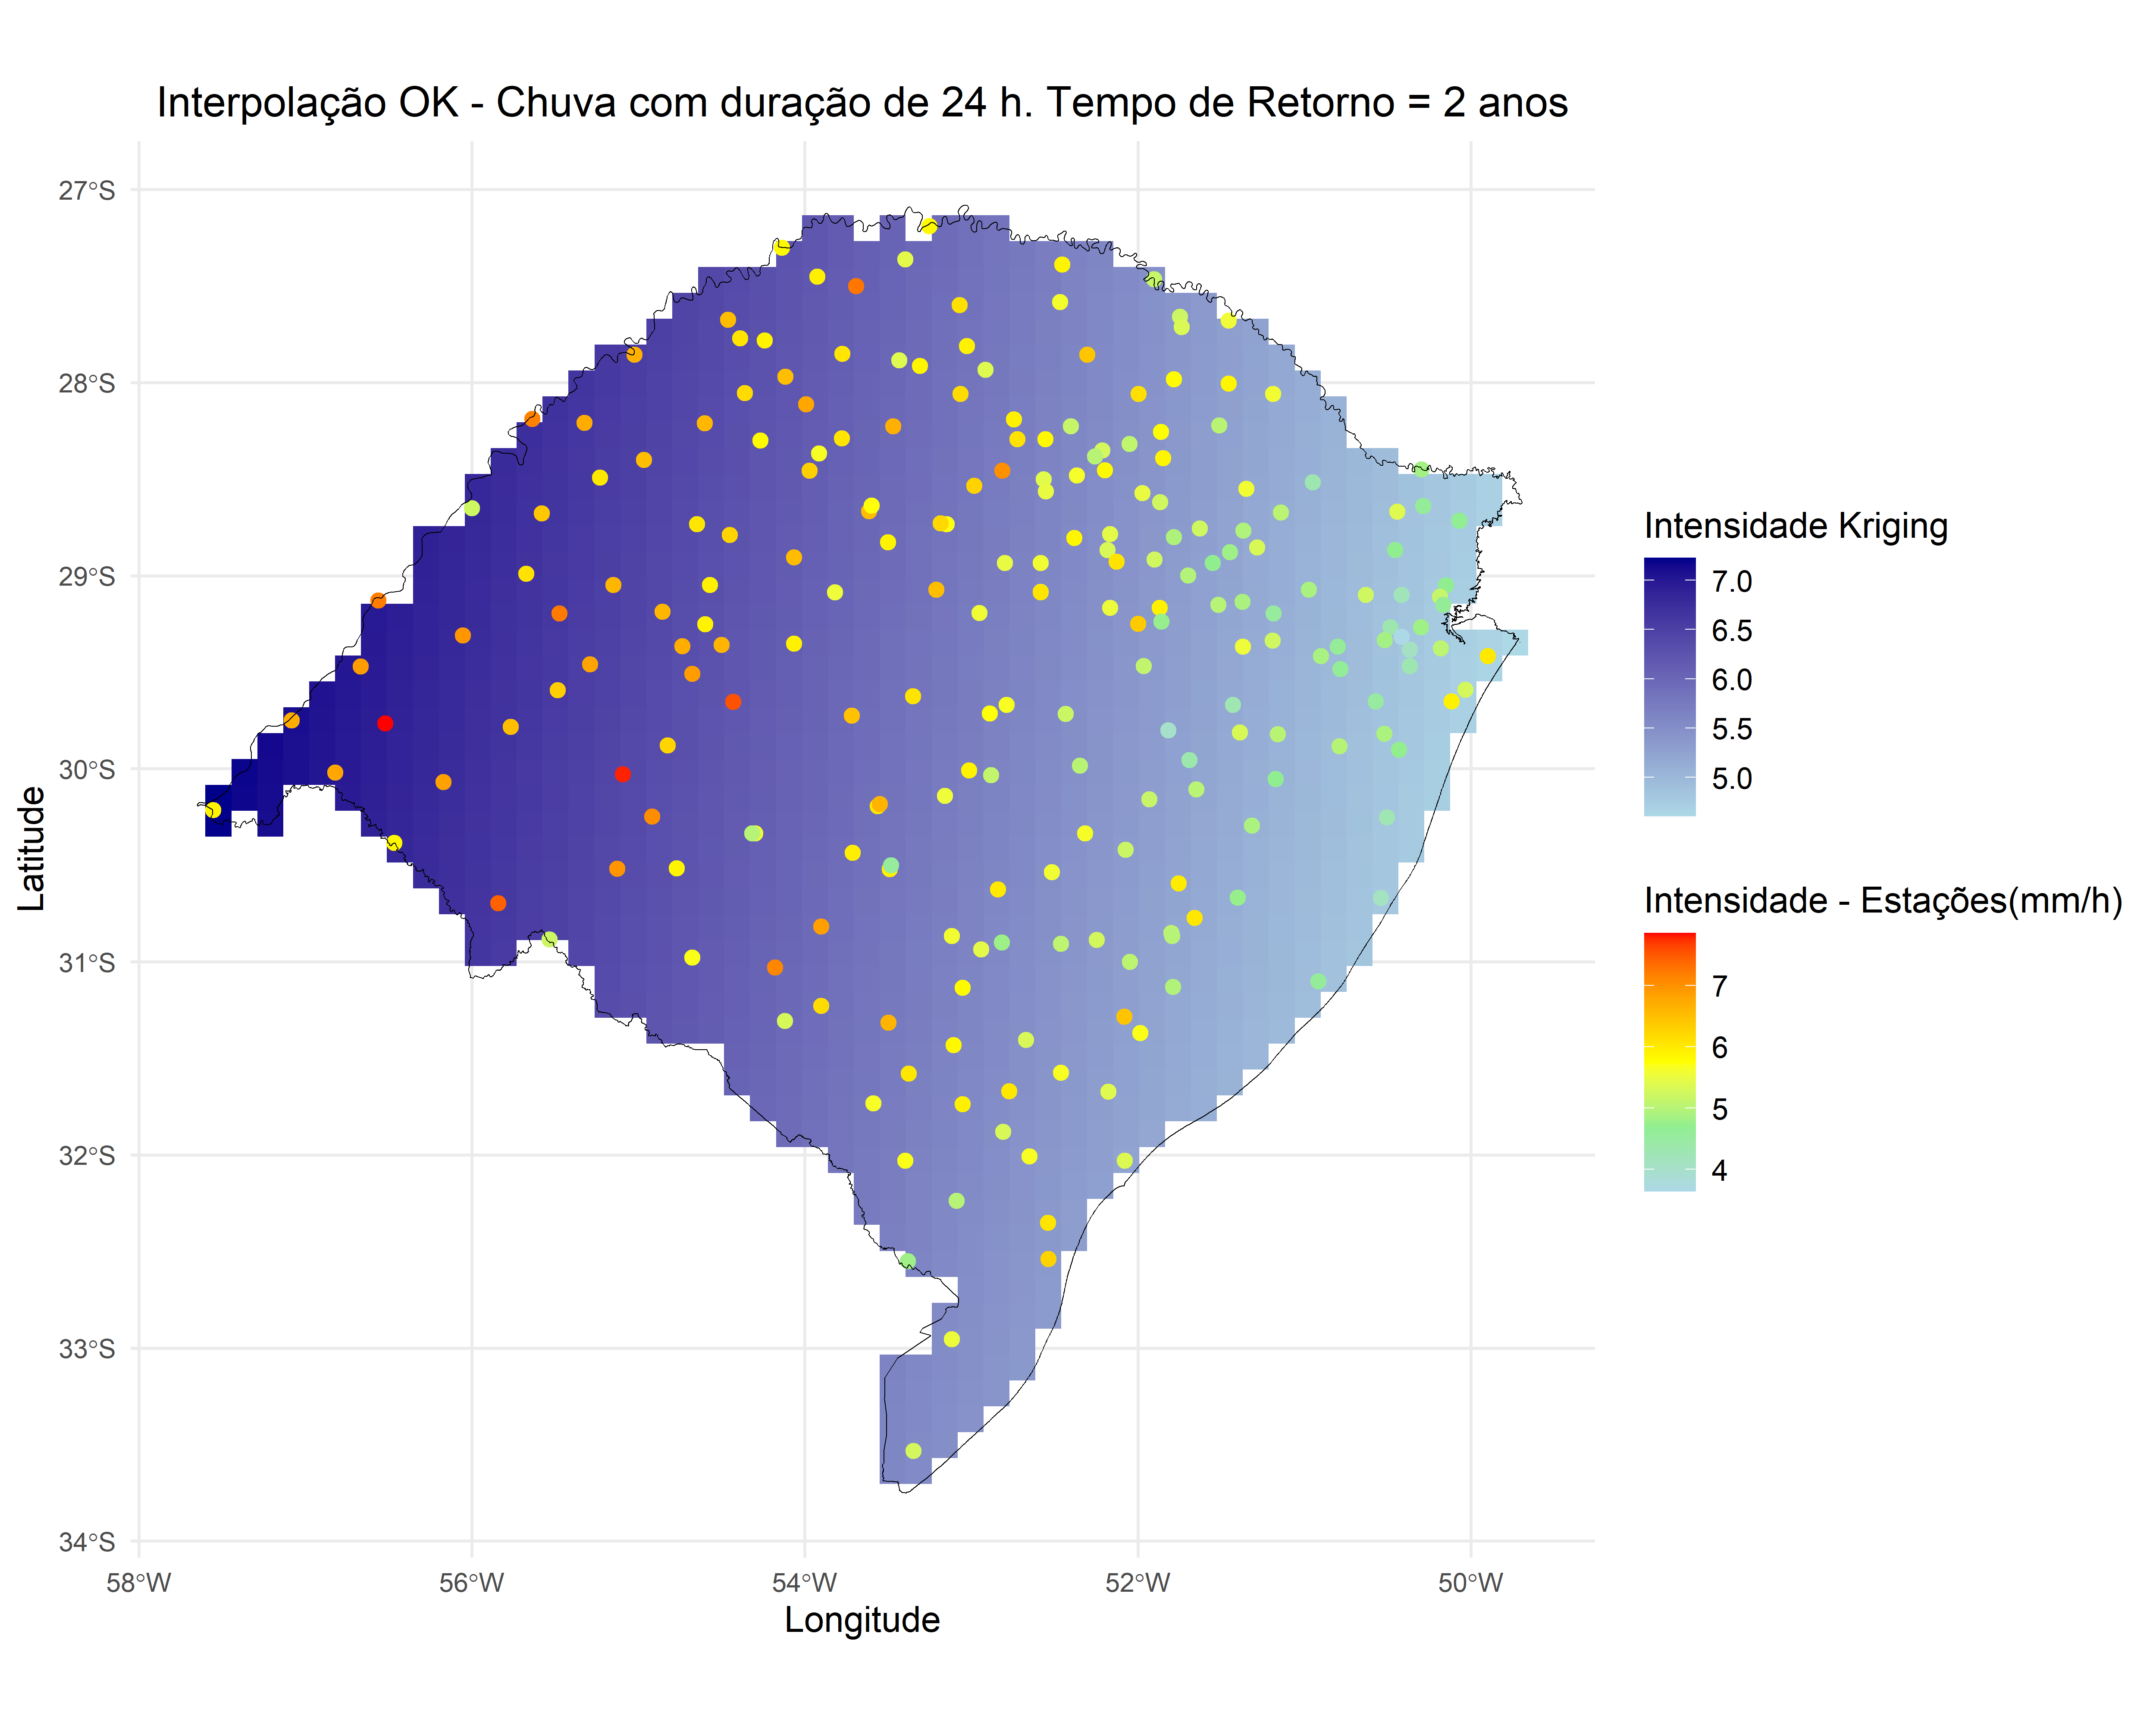
\includegraphics{Figuras/Figura11b.png}

}

\subcaption{\label{fig-Figura11b}Espacialização por OK. Tempo de Retorno
=5 anos}

\end{minipage}%
\newline
\begin{minipage}{\linewidth}
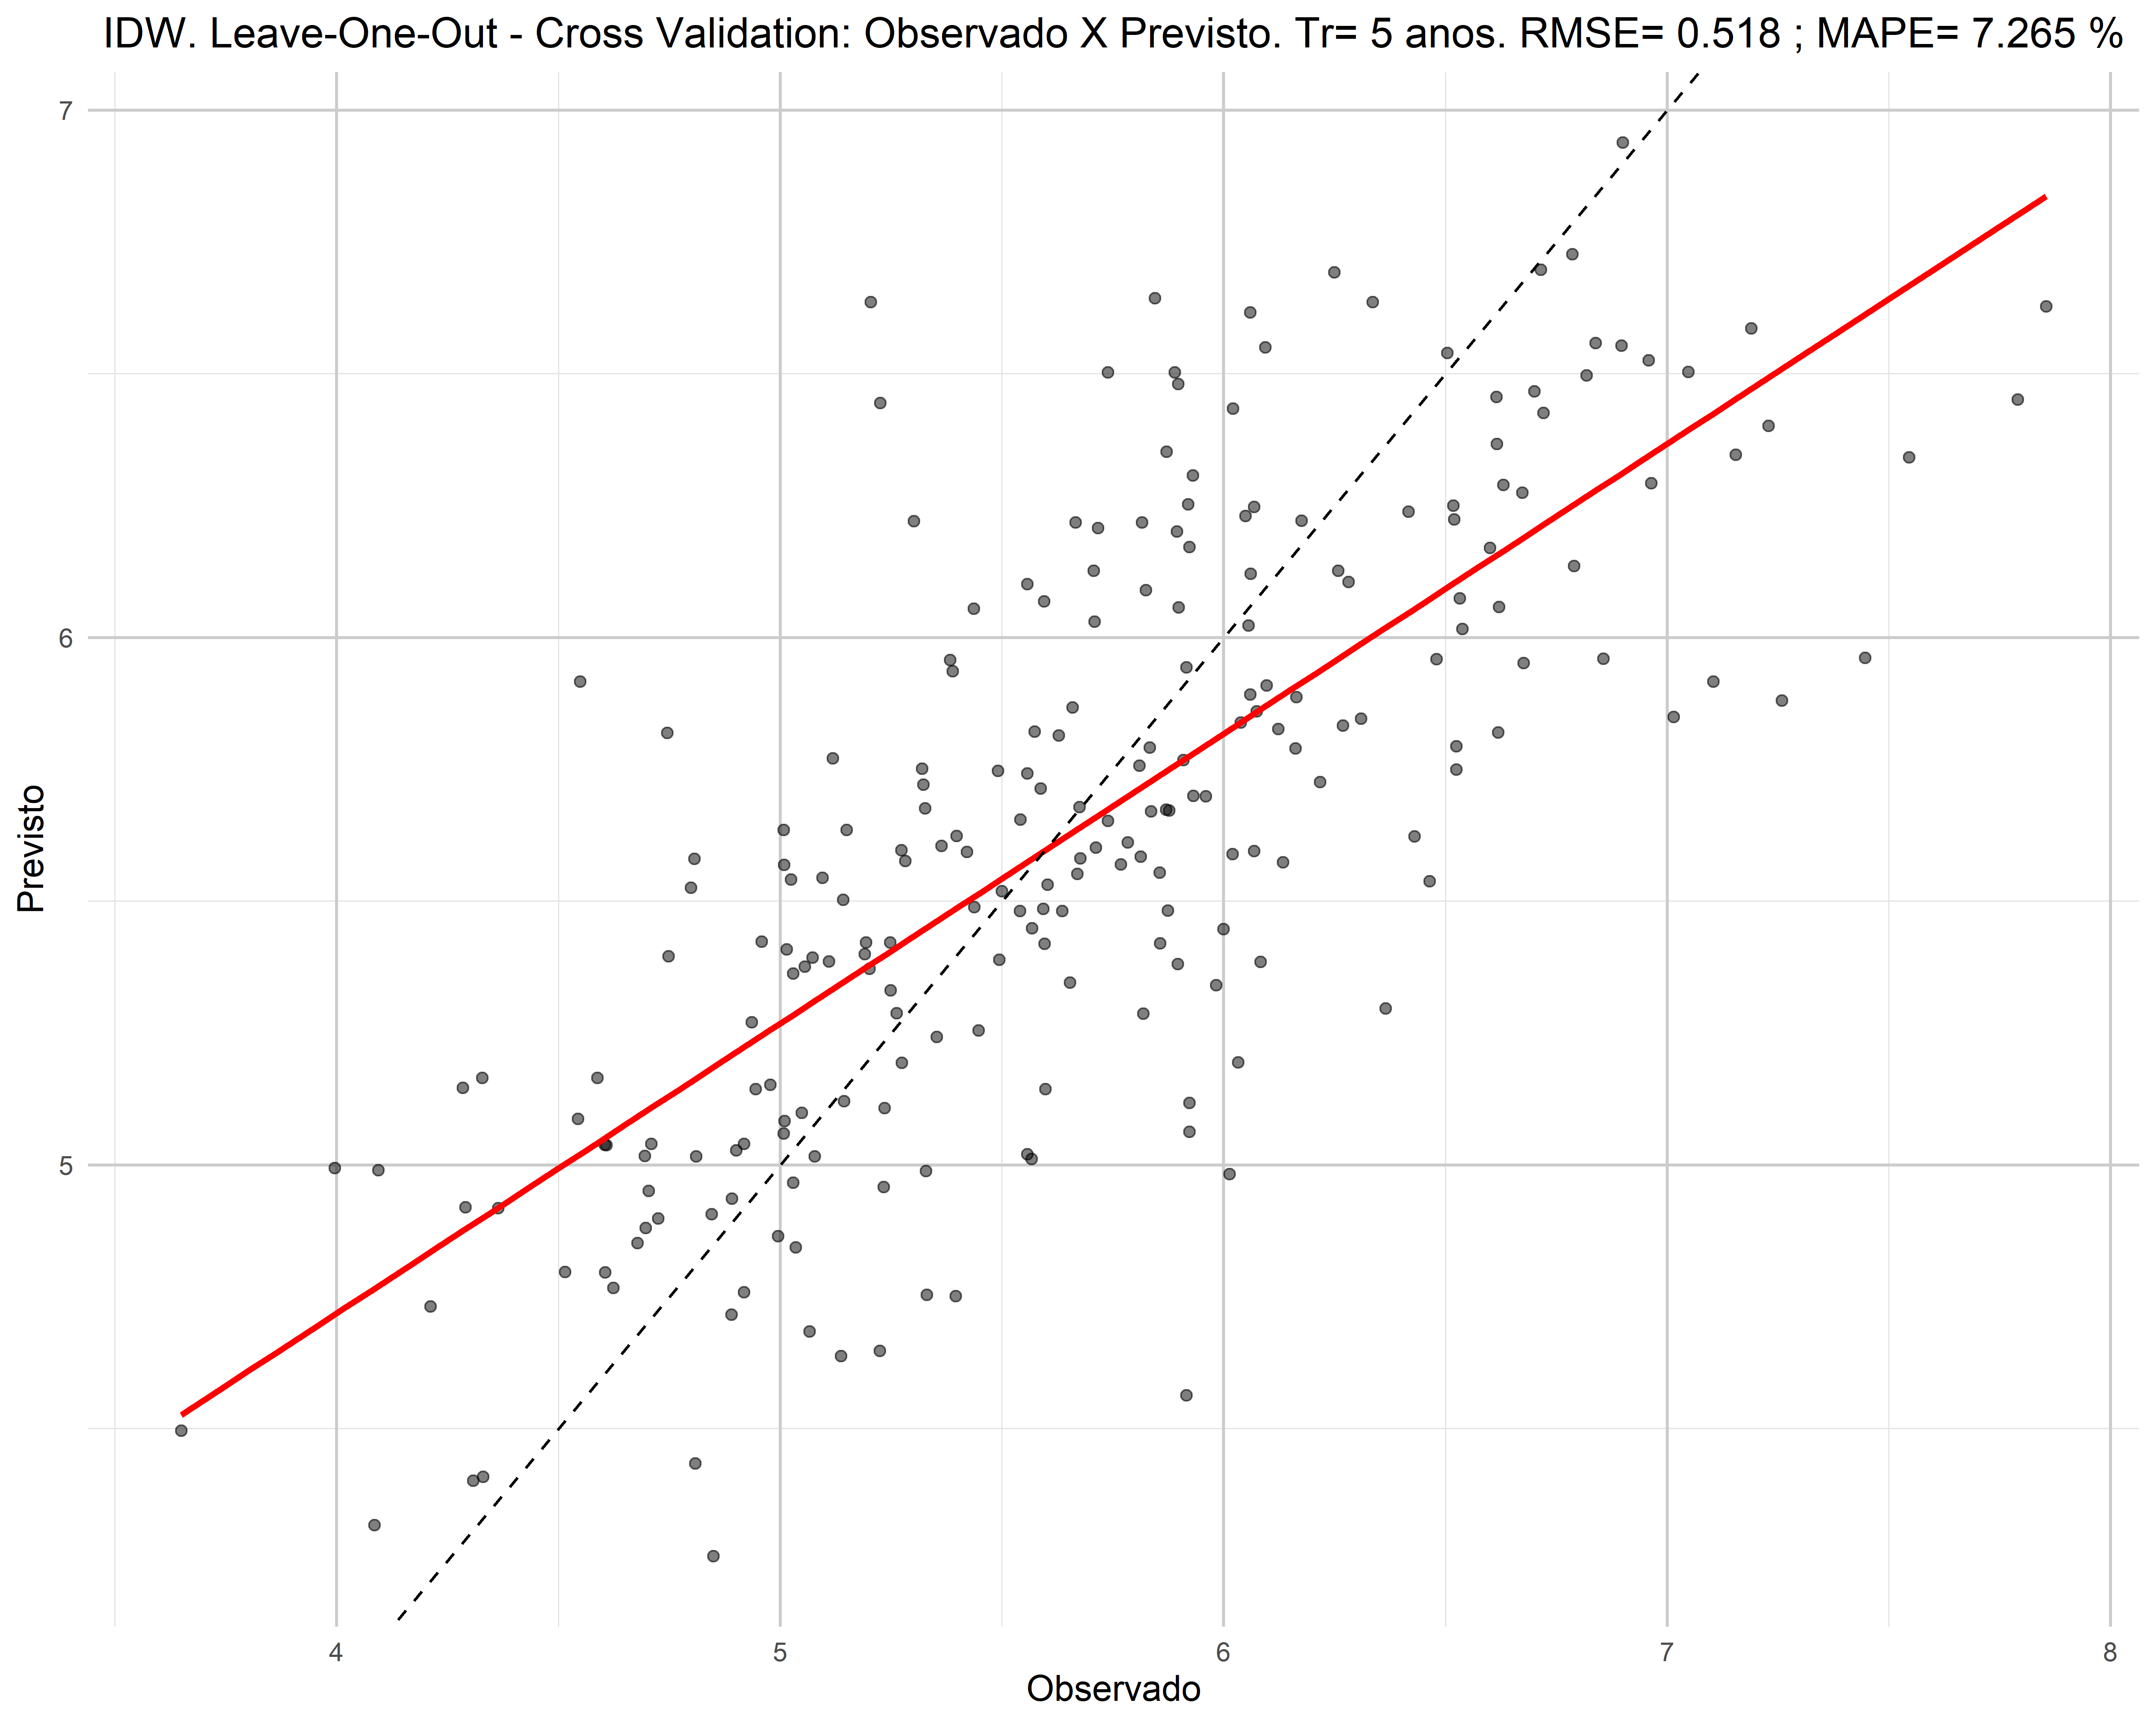
\includegraphics{Figuras/Figura11c.png}
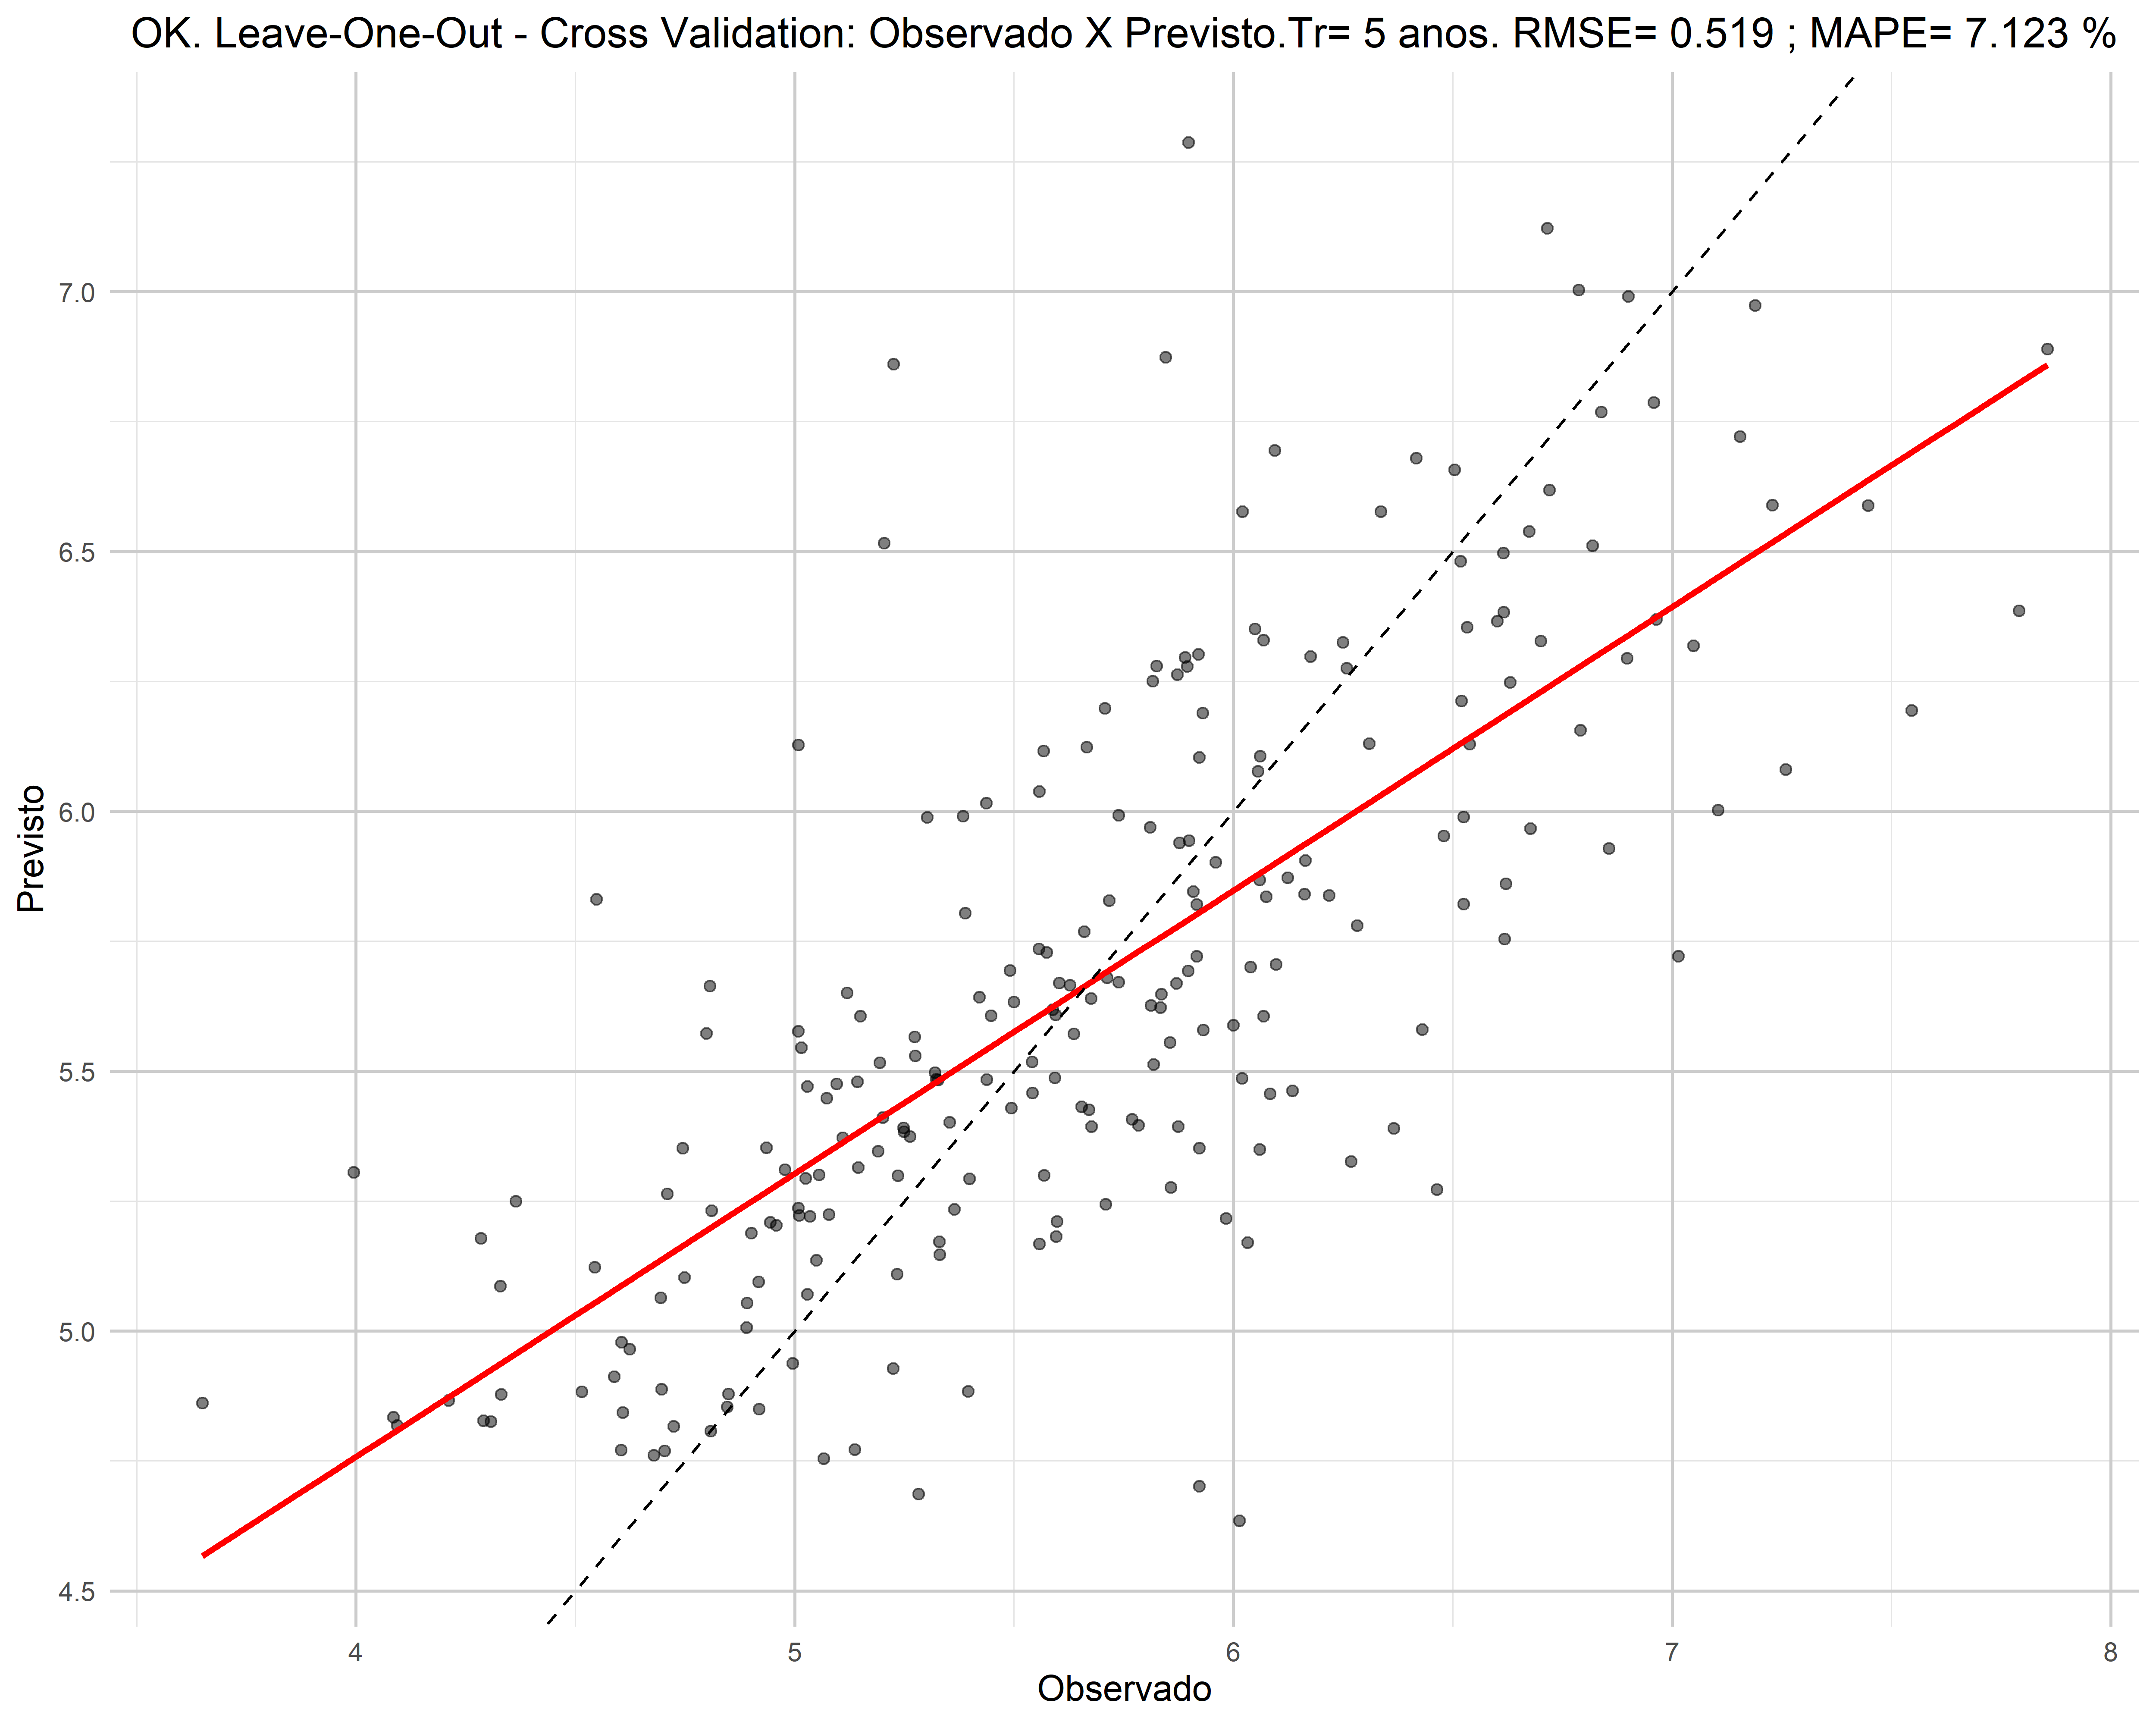
\includegraphics{Figuras/Figura11d.png}\end{minipage}%

\caption{\label{fig-Figura11}Resultados obtidos para intensidade da
chuva de duração de 24 h e tempo de retorno de 5 anos para interpolação
por IDW (a) e por krigagem ordinária, OK (b). Valores preditos em função
dos valores observados e resultados das métricas RMSE e MAPE para
interpolação por IDW (c) e OK (d).}

\end{figure}%

\begin{figure}

\begin{minipage}{\linewidth}

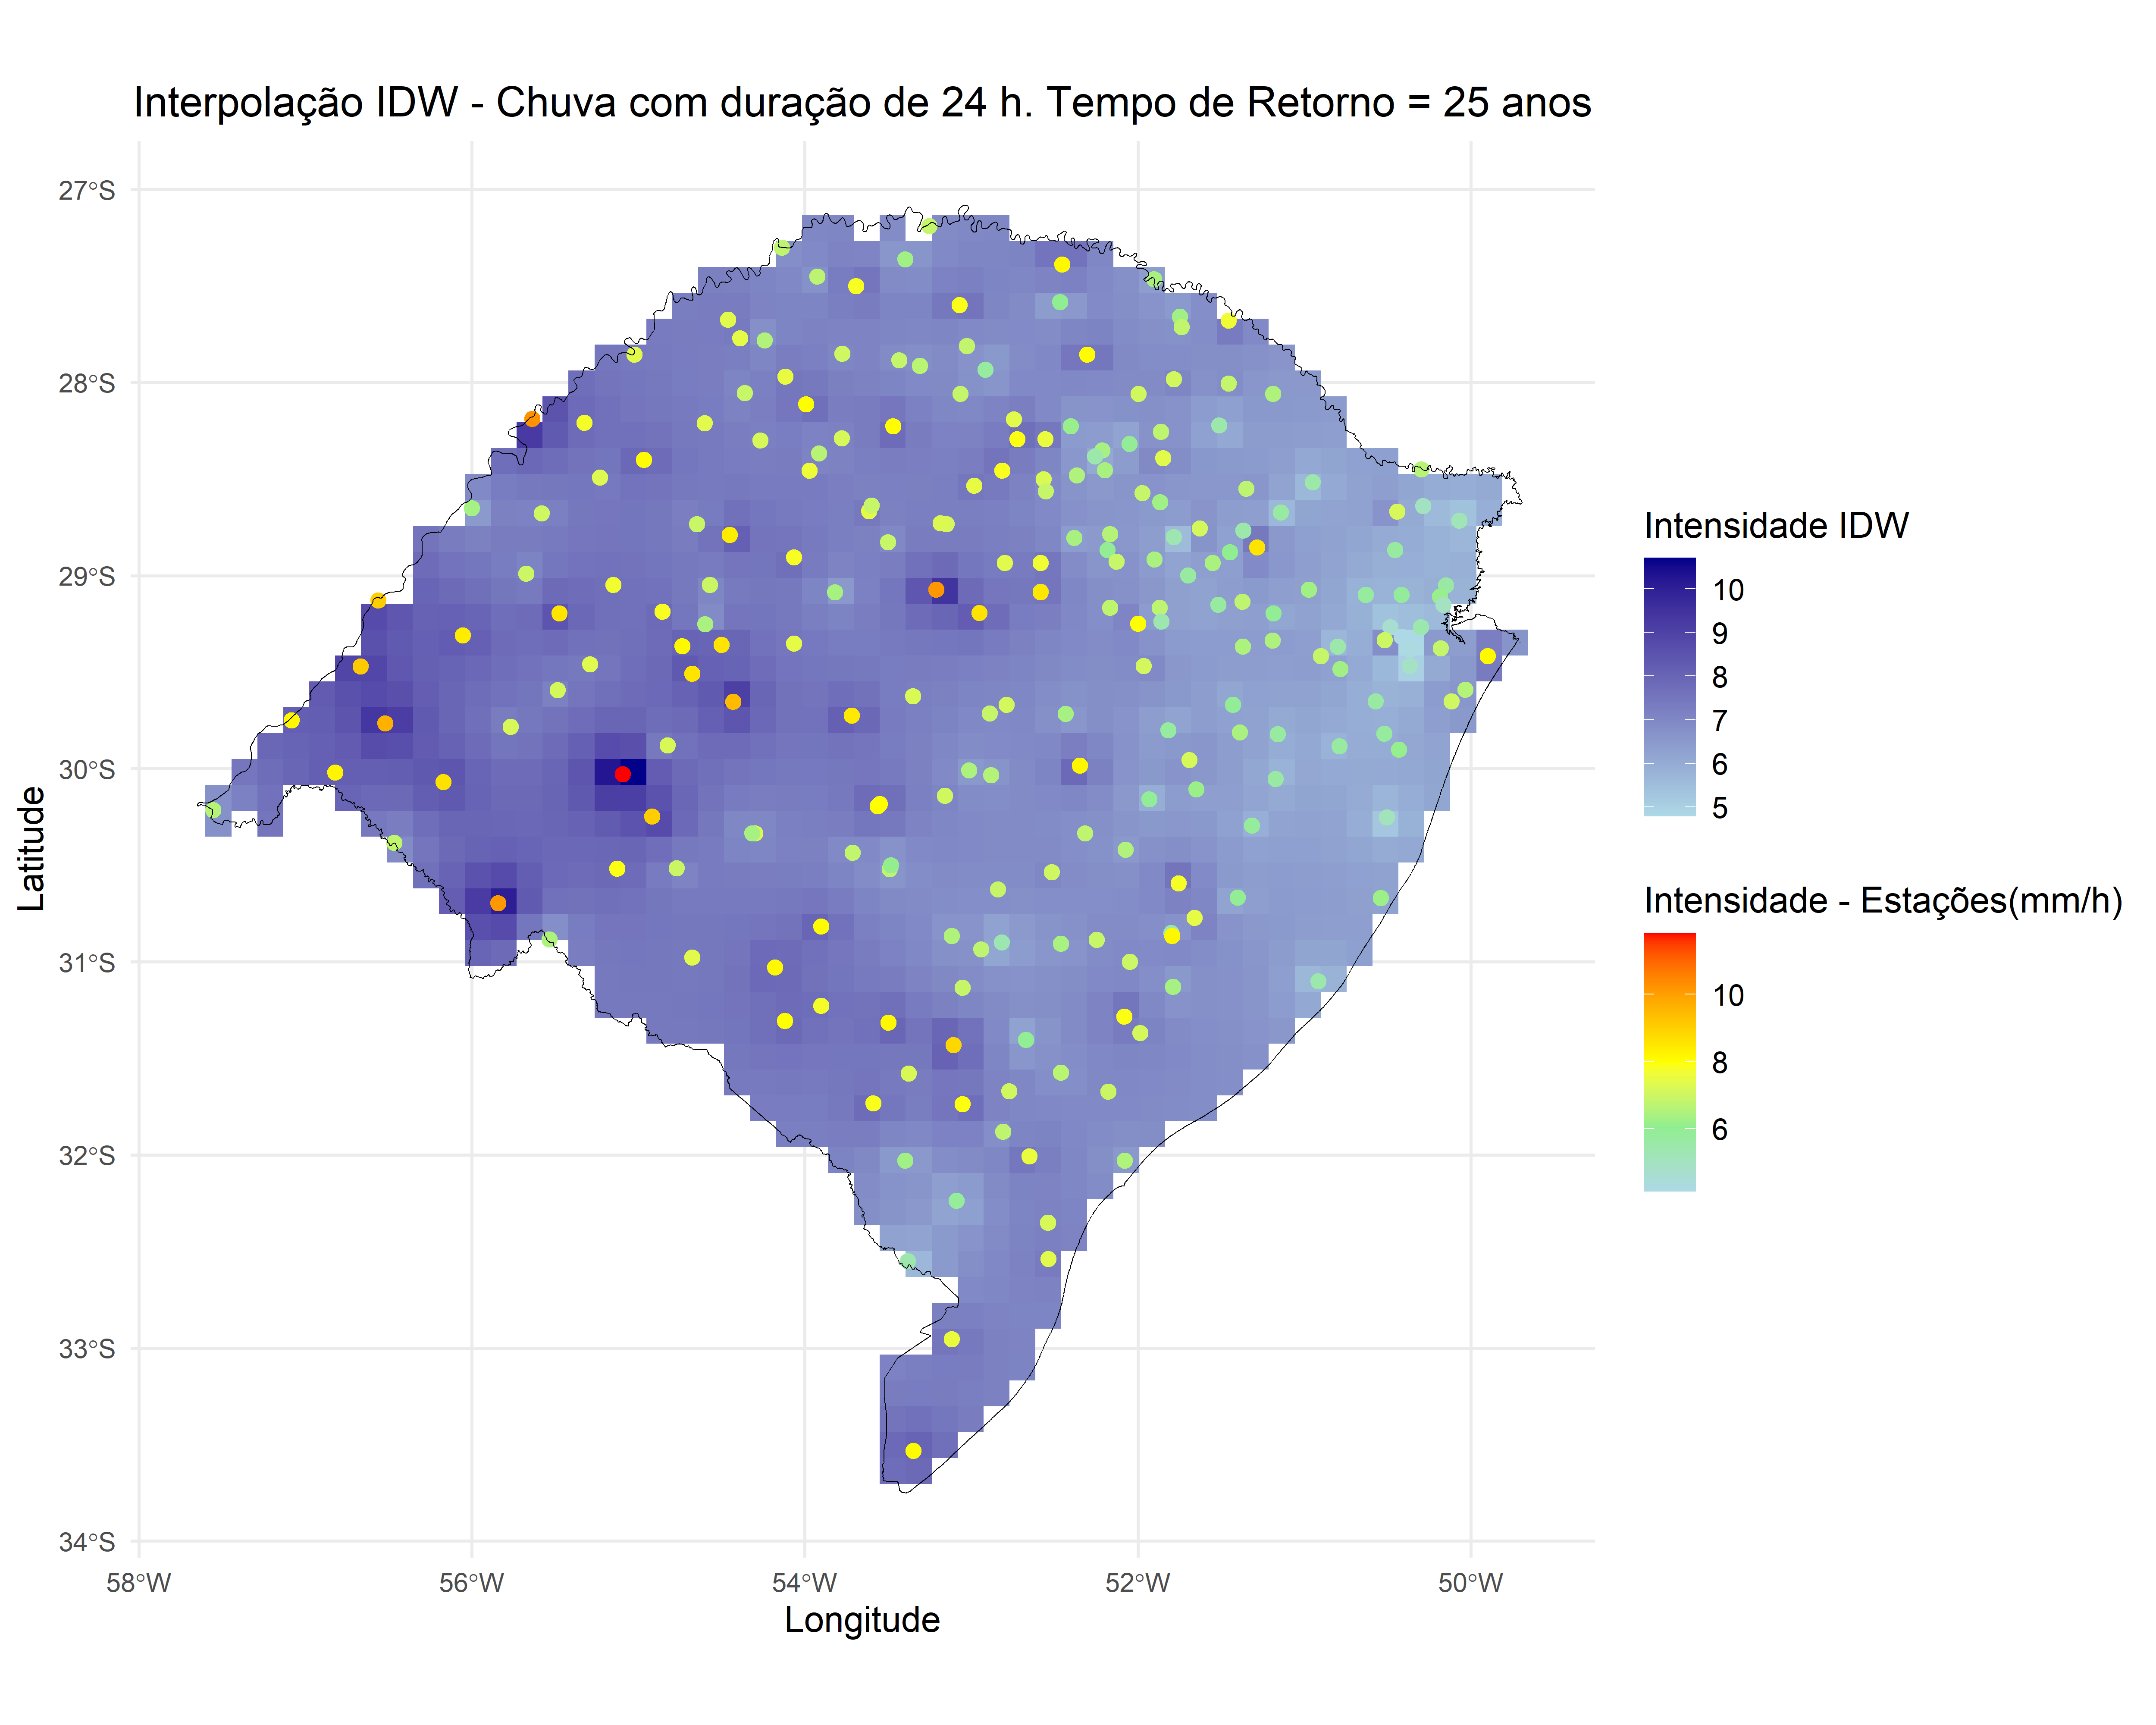
\includegraphics{Figuras/Figura12a.png}

\subcaption{\label{}Espacialização por IDW (p=2). Tempo de Retorno =25
anos}
\end{minipage}%
\newline
\begin{minipage}{\linewidth}

\centering{

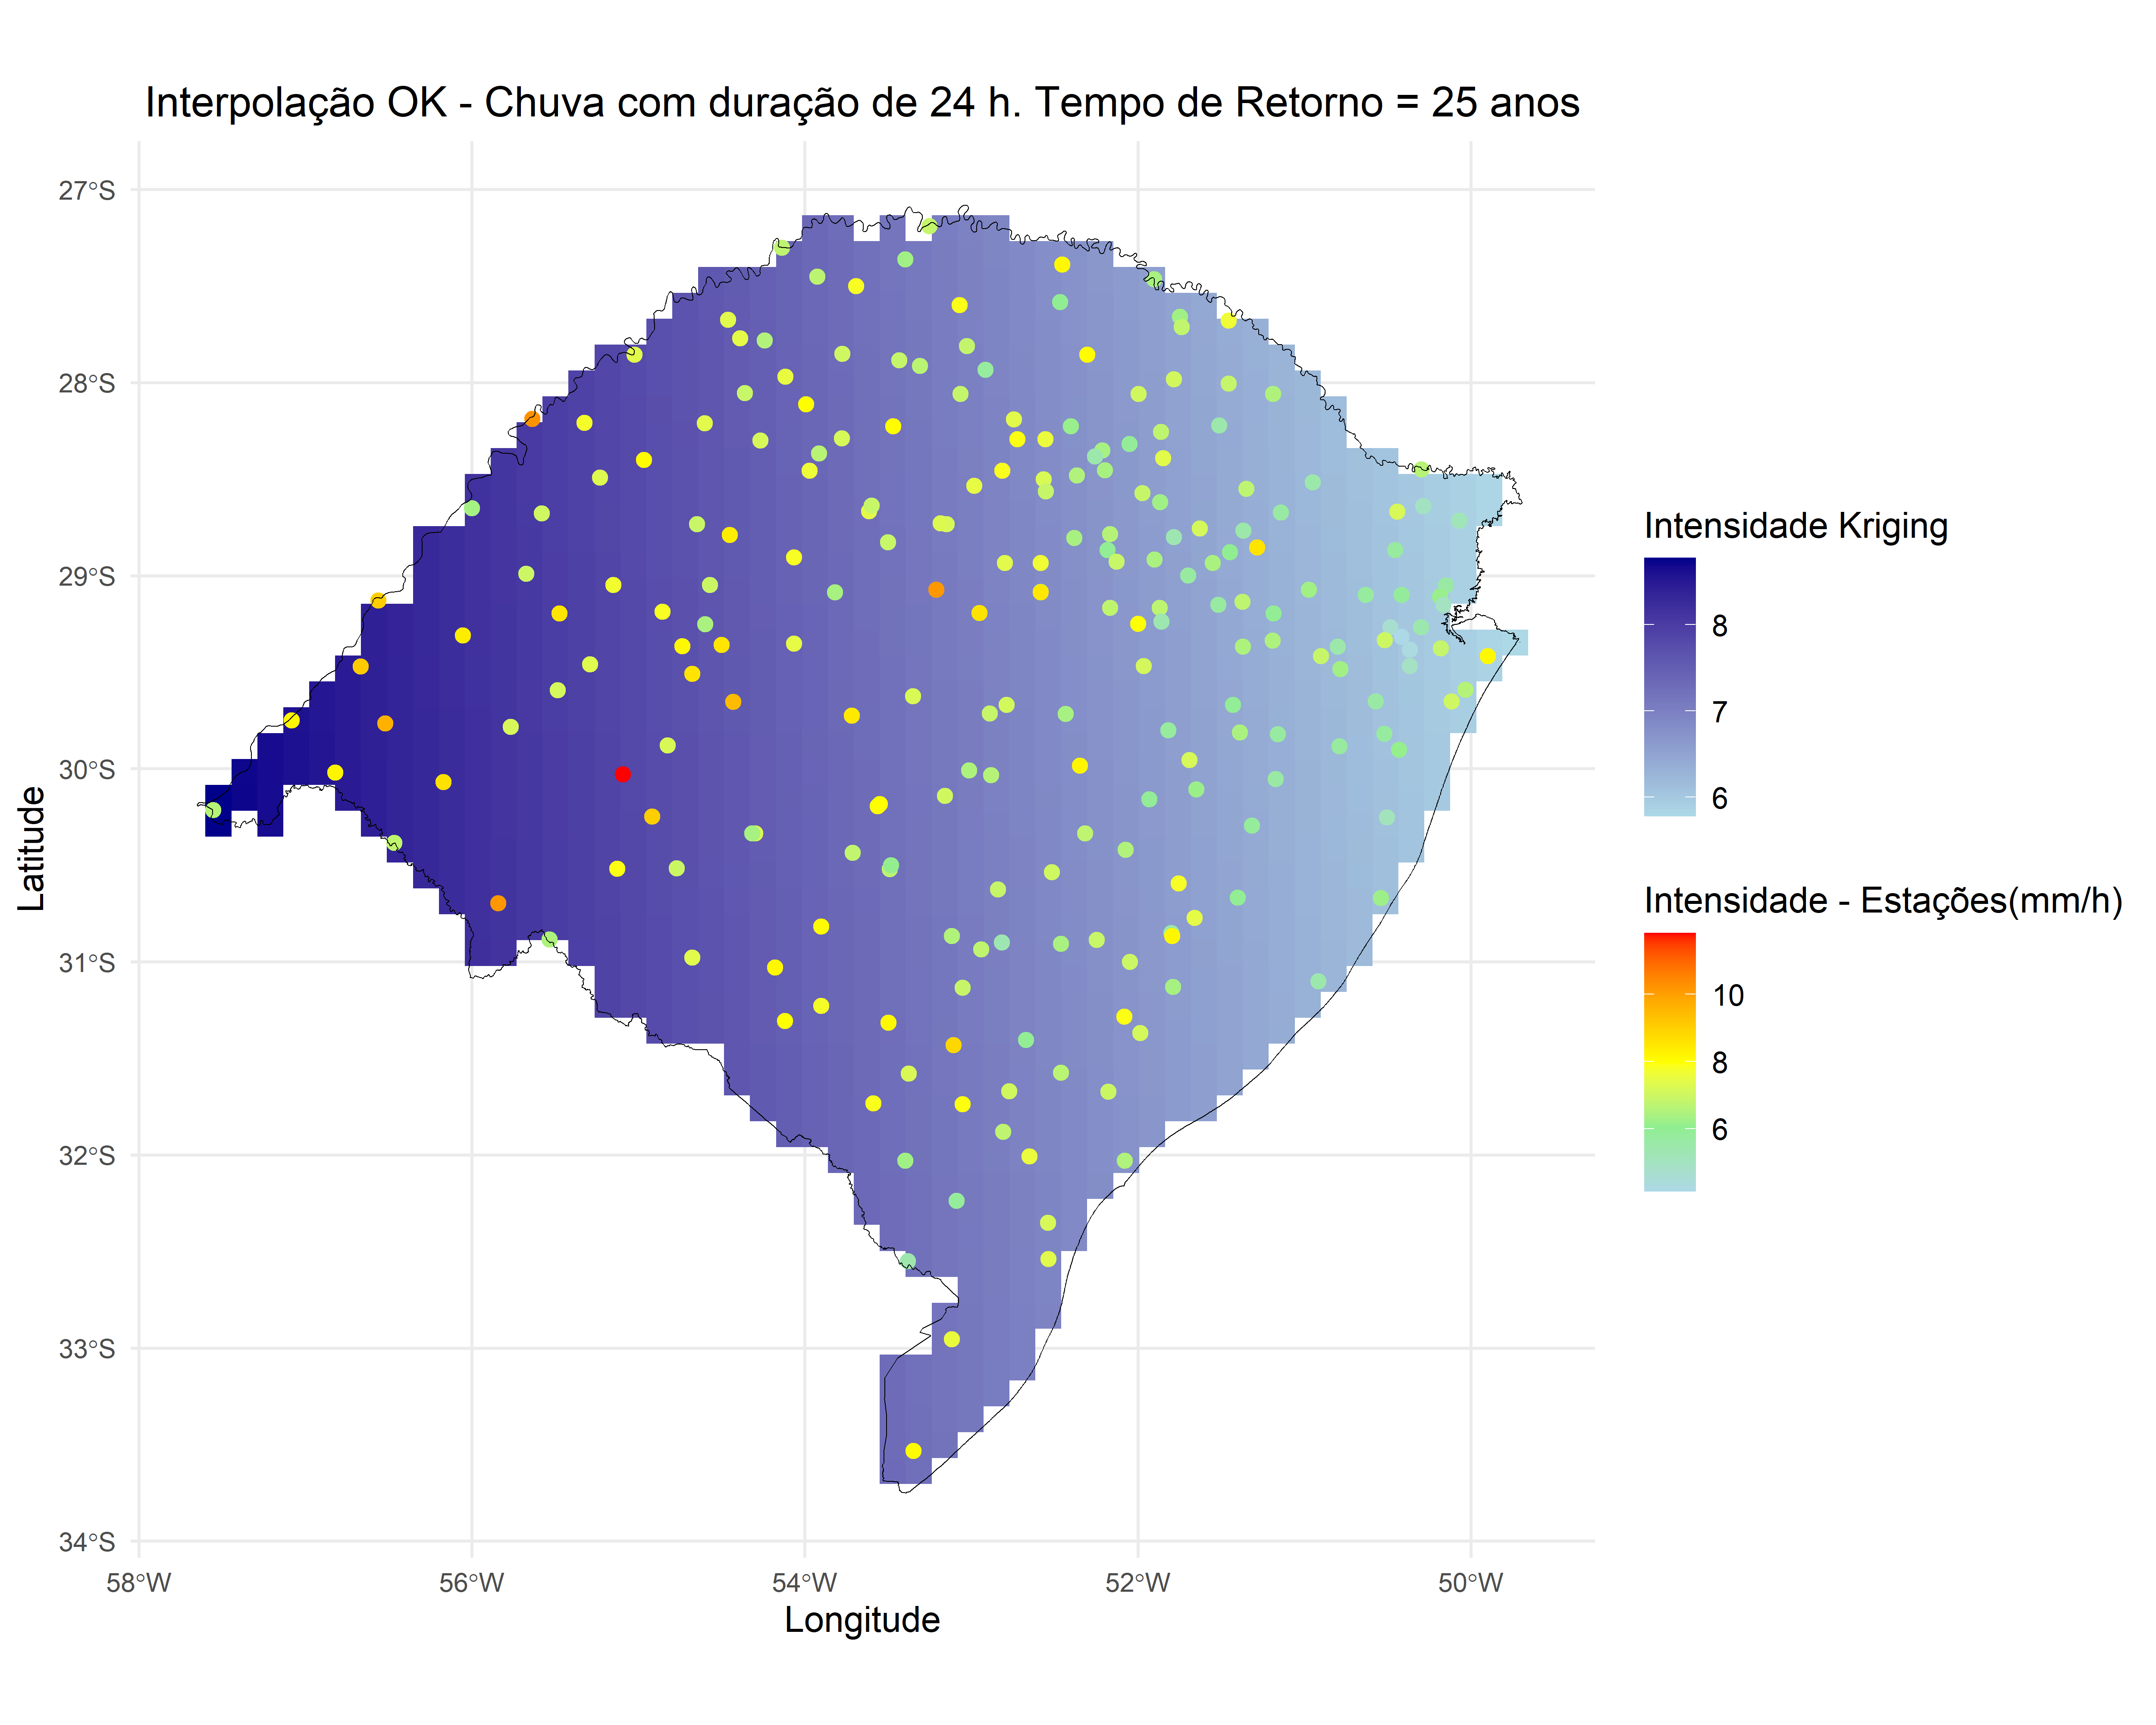
\includegraphics{Figuras/Figura12b.png}

}

\subcaption{\label{fig-Figura12b}Espacialização por OK. Tempo de Retorno
=25 anos}

\end{minipage}%
\newline
\begin{minipage}{\linewidth}
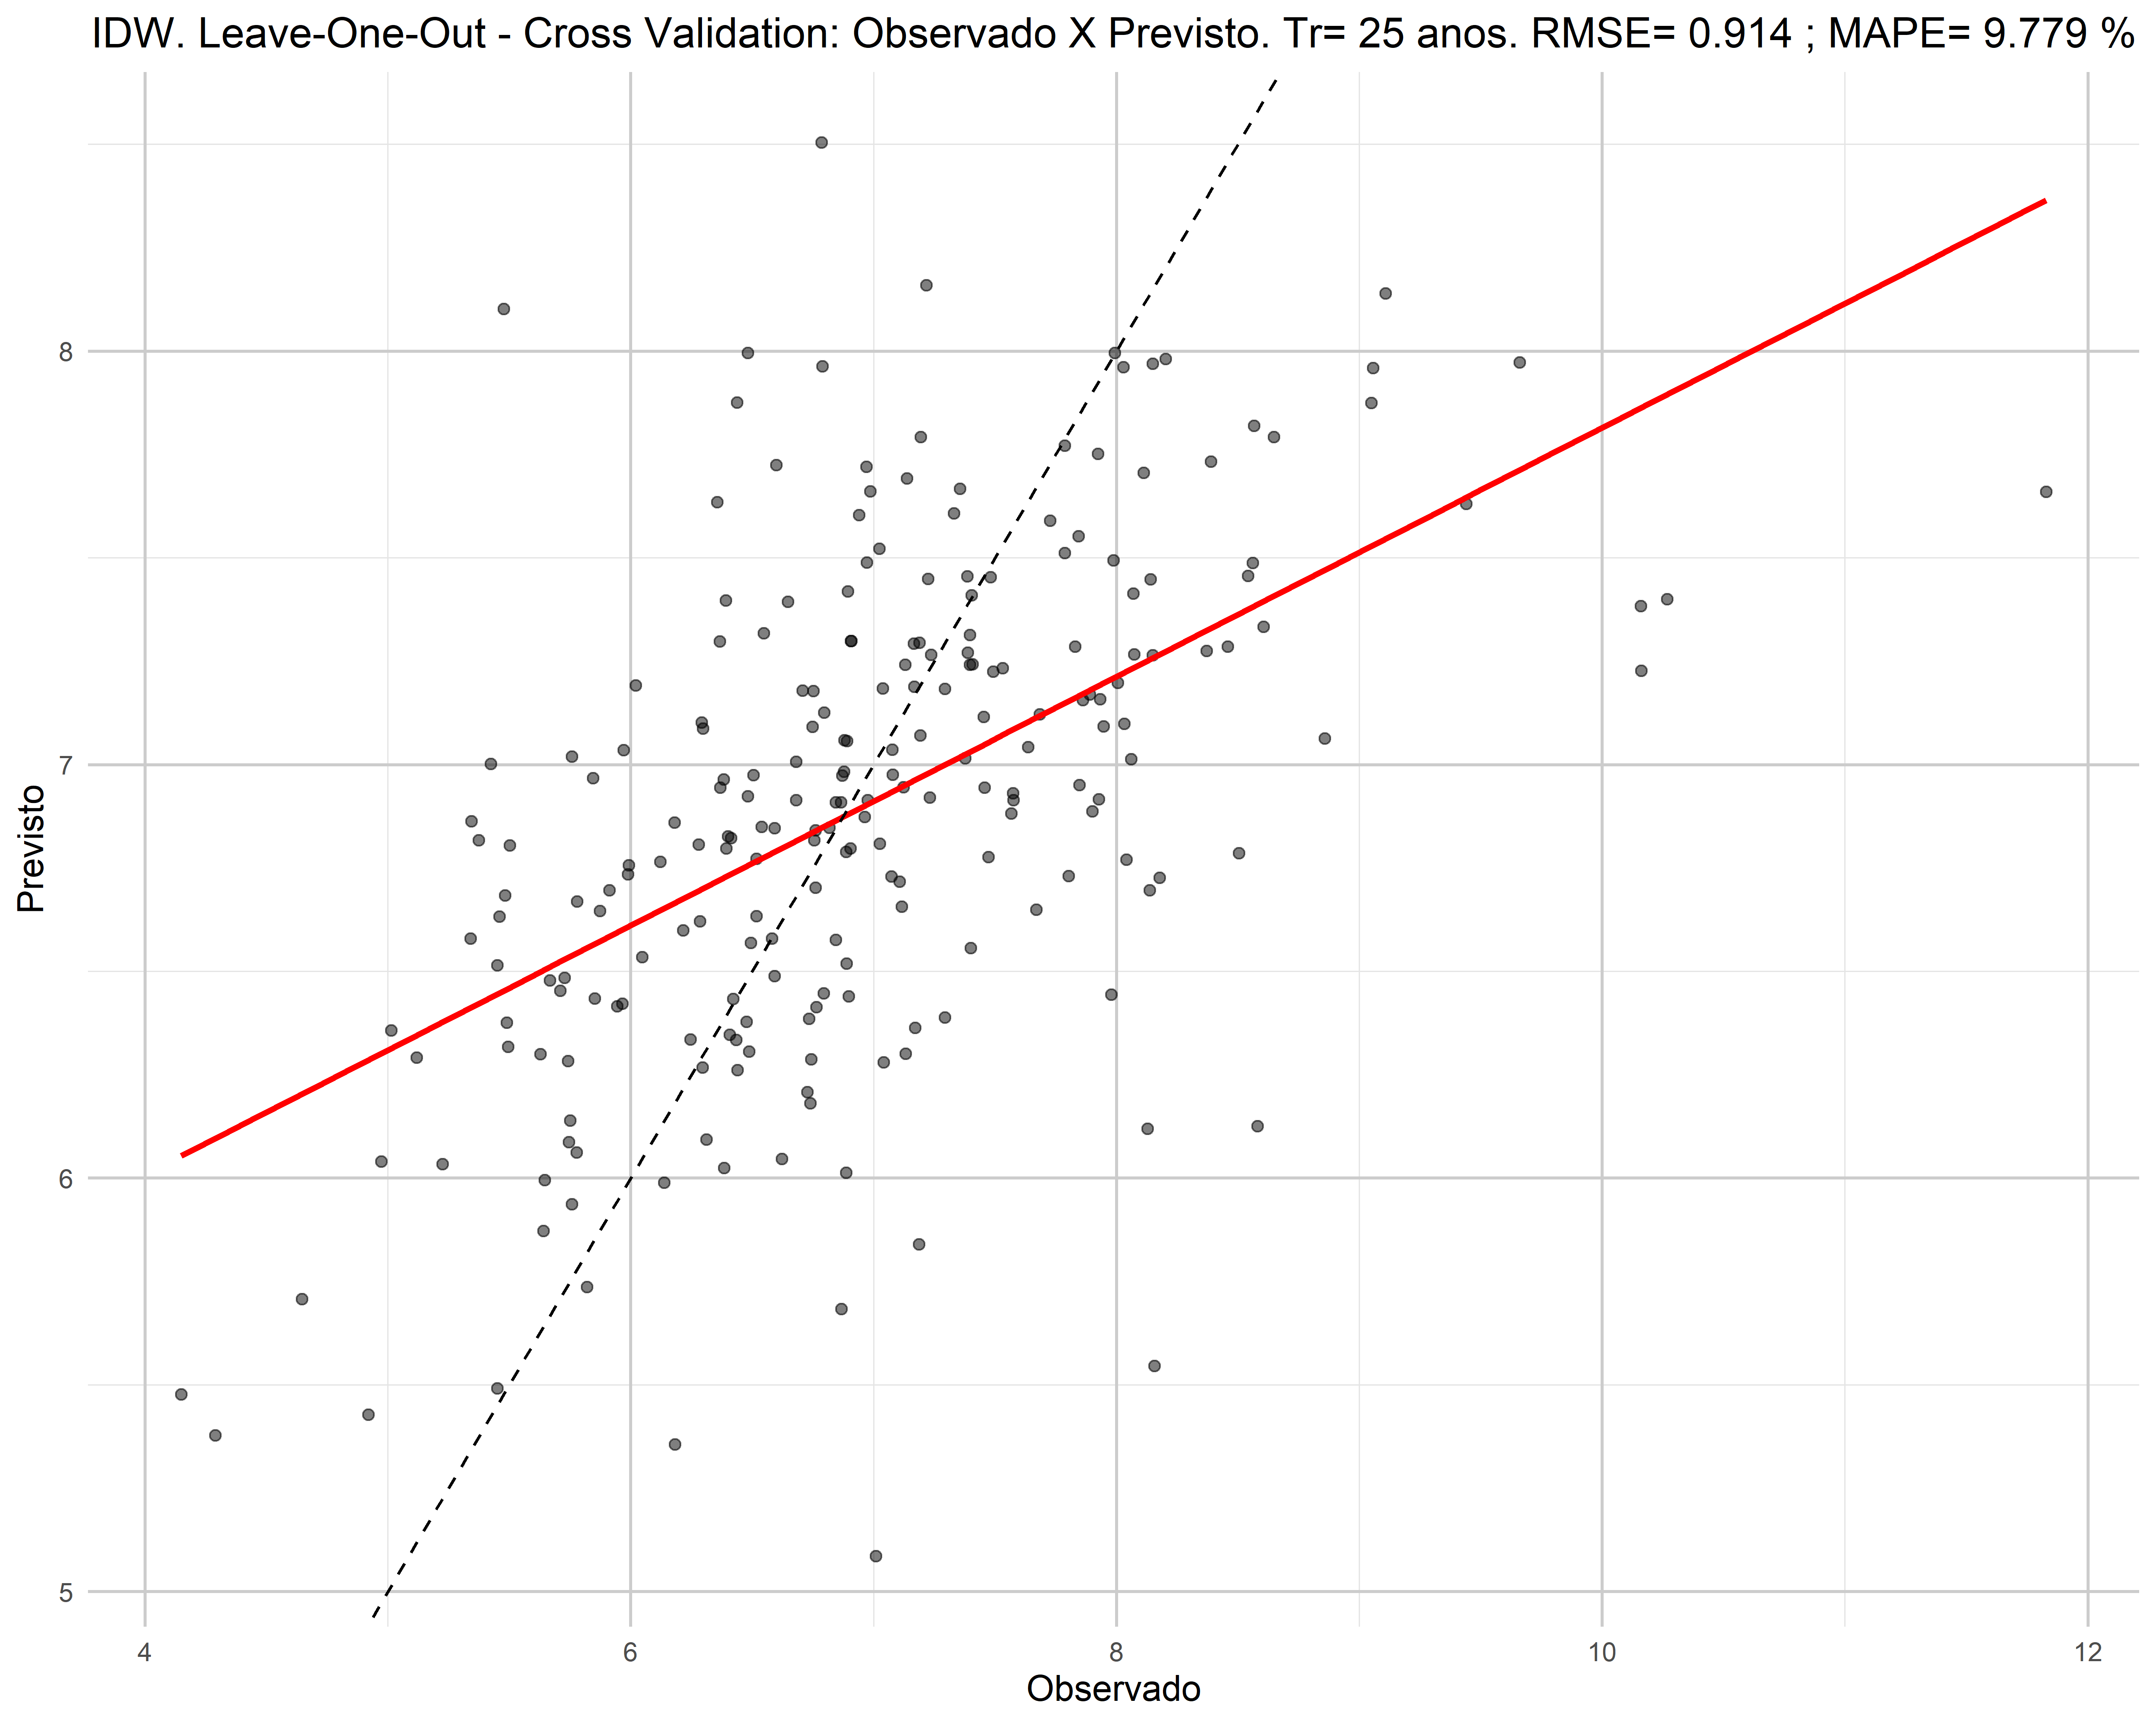
\includegraphics{Figuras/Figura12c.png}
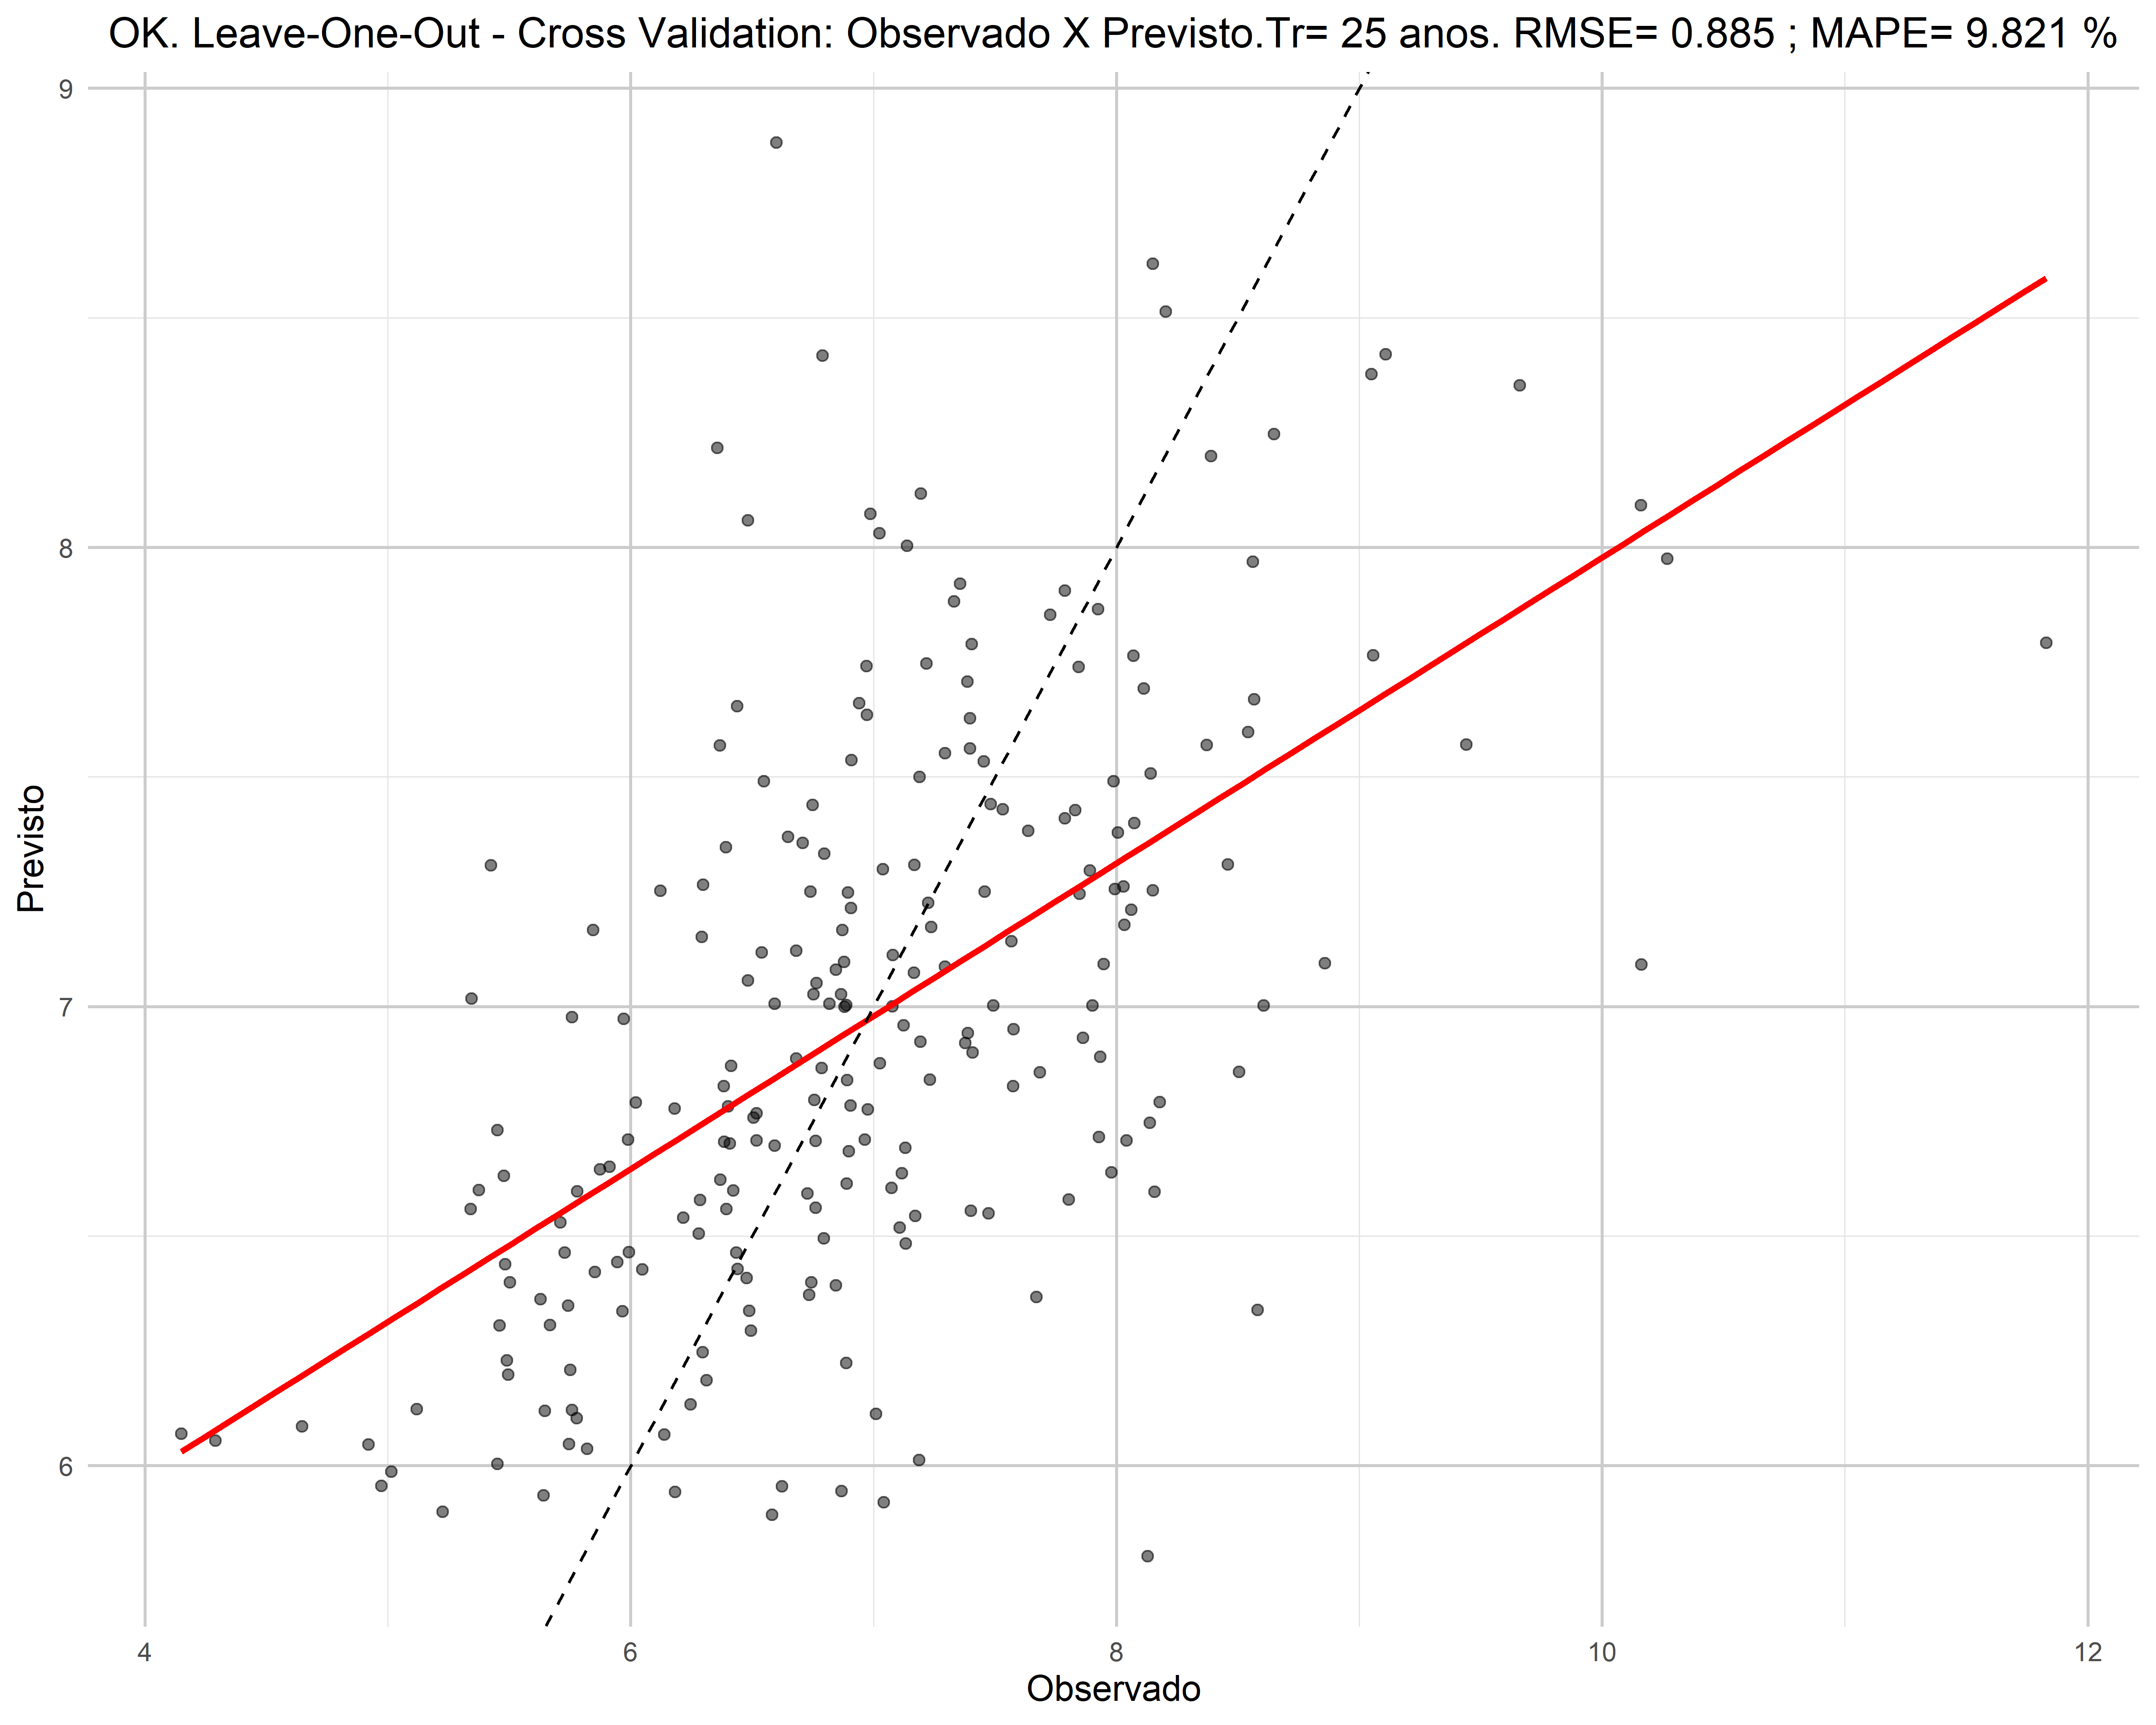
\includegraphics{Figuras/Figura12d.png}\end{minipage}%

\caption{\label{fig-Figura12}Resultados obtidos para intensidade da
chuva de duração de 24 h e tempo de retorno de 25 anos para interpolação
por IDW (a) e por krigagem ordinária, OK (b). Valores preditos em função
dos valores observados e resultados das métricas RMSE e MAPE para
interpolação por IDW (c) e OK (d).}

\end{figure}%

\begin{figure}

\begin{minipage}{\linewidth}

\centering{

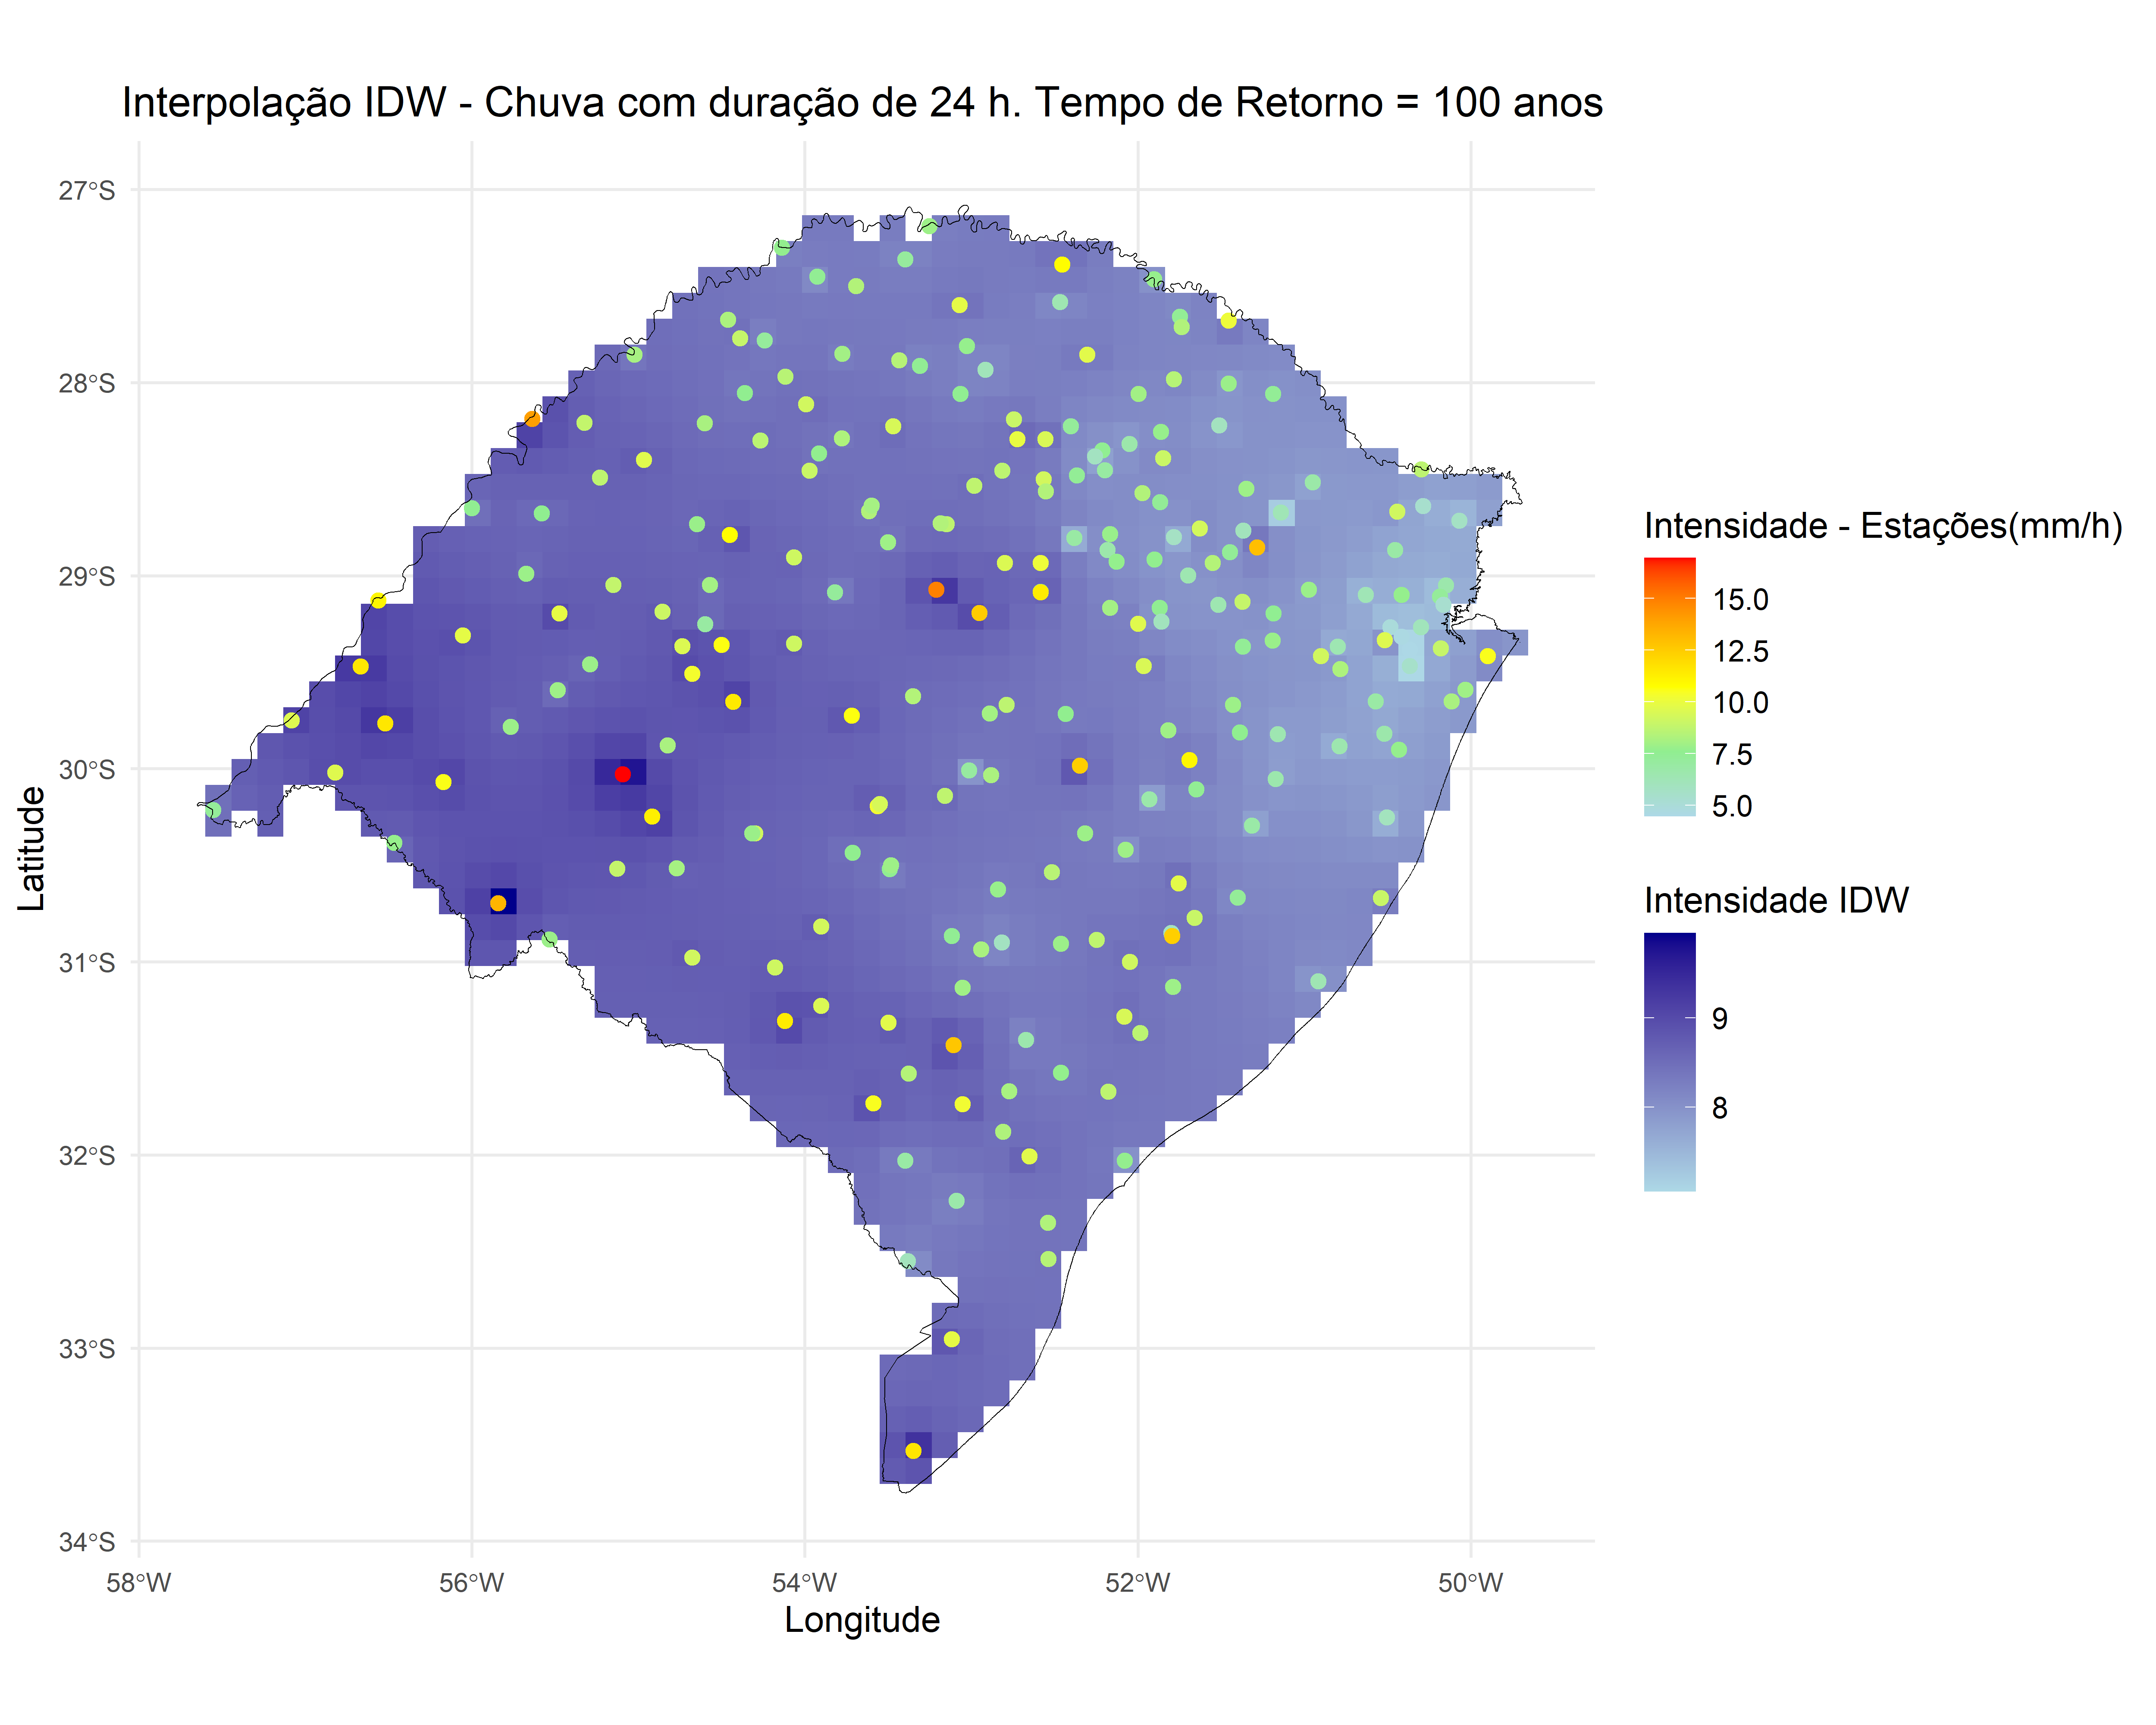
\includegraphics{Figuras/Figura13a.png}

}

\subcaption{\label{fig-Figura13a}Espacialização por IDW (p=1). Tempo de
Retorno =100 anos}

\end{minipage}%
\newline
\begin{minipage}{\linewidth}

\centering{

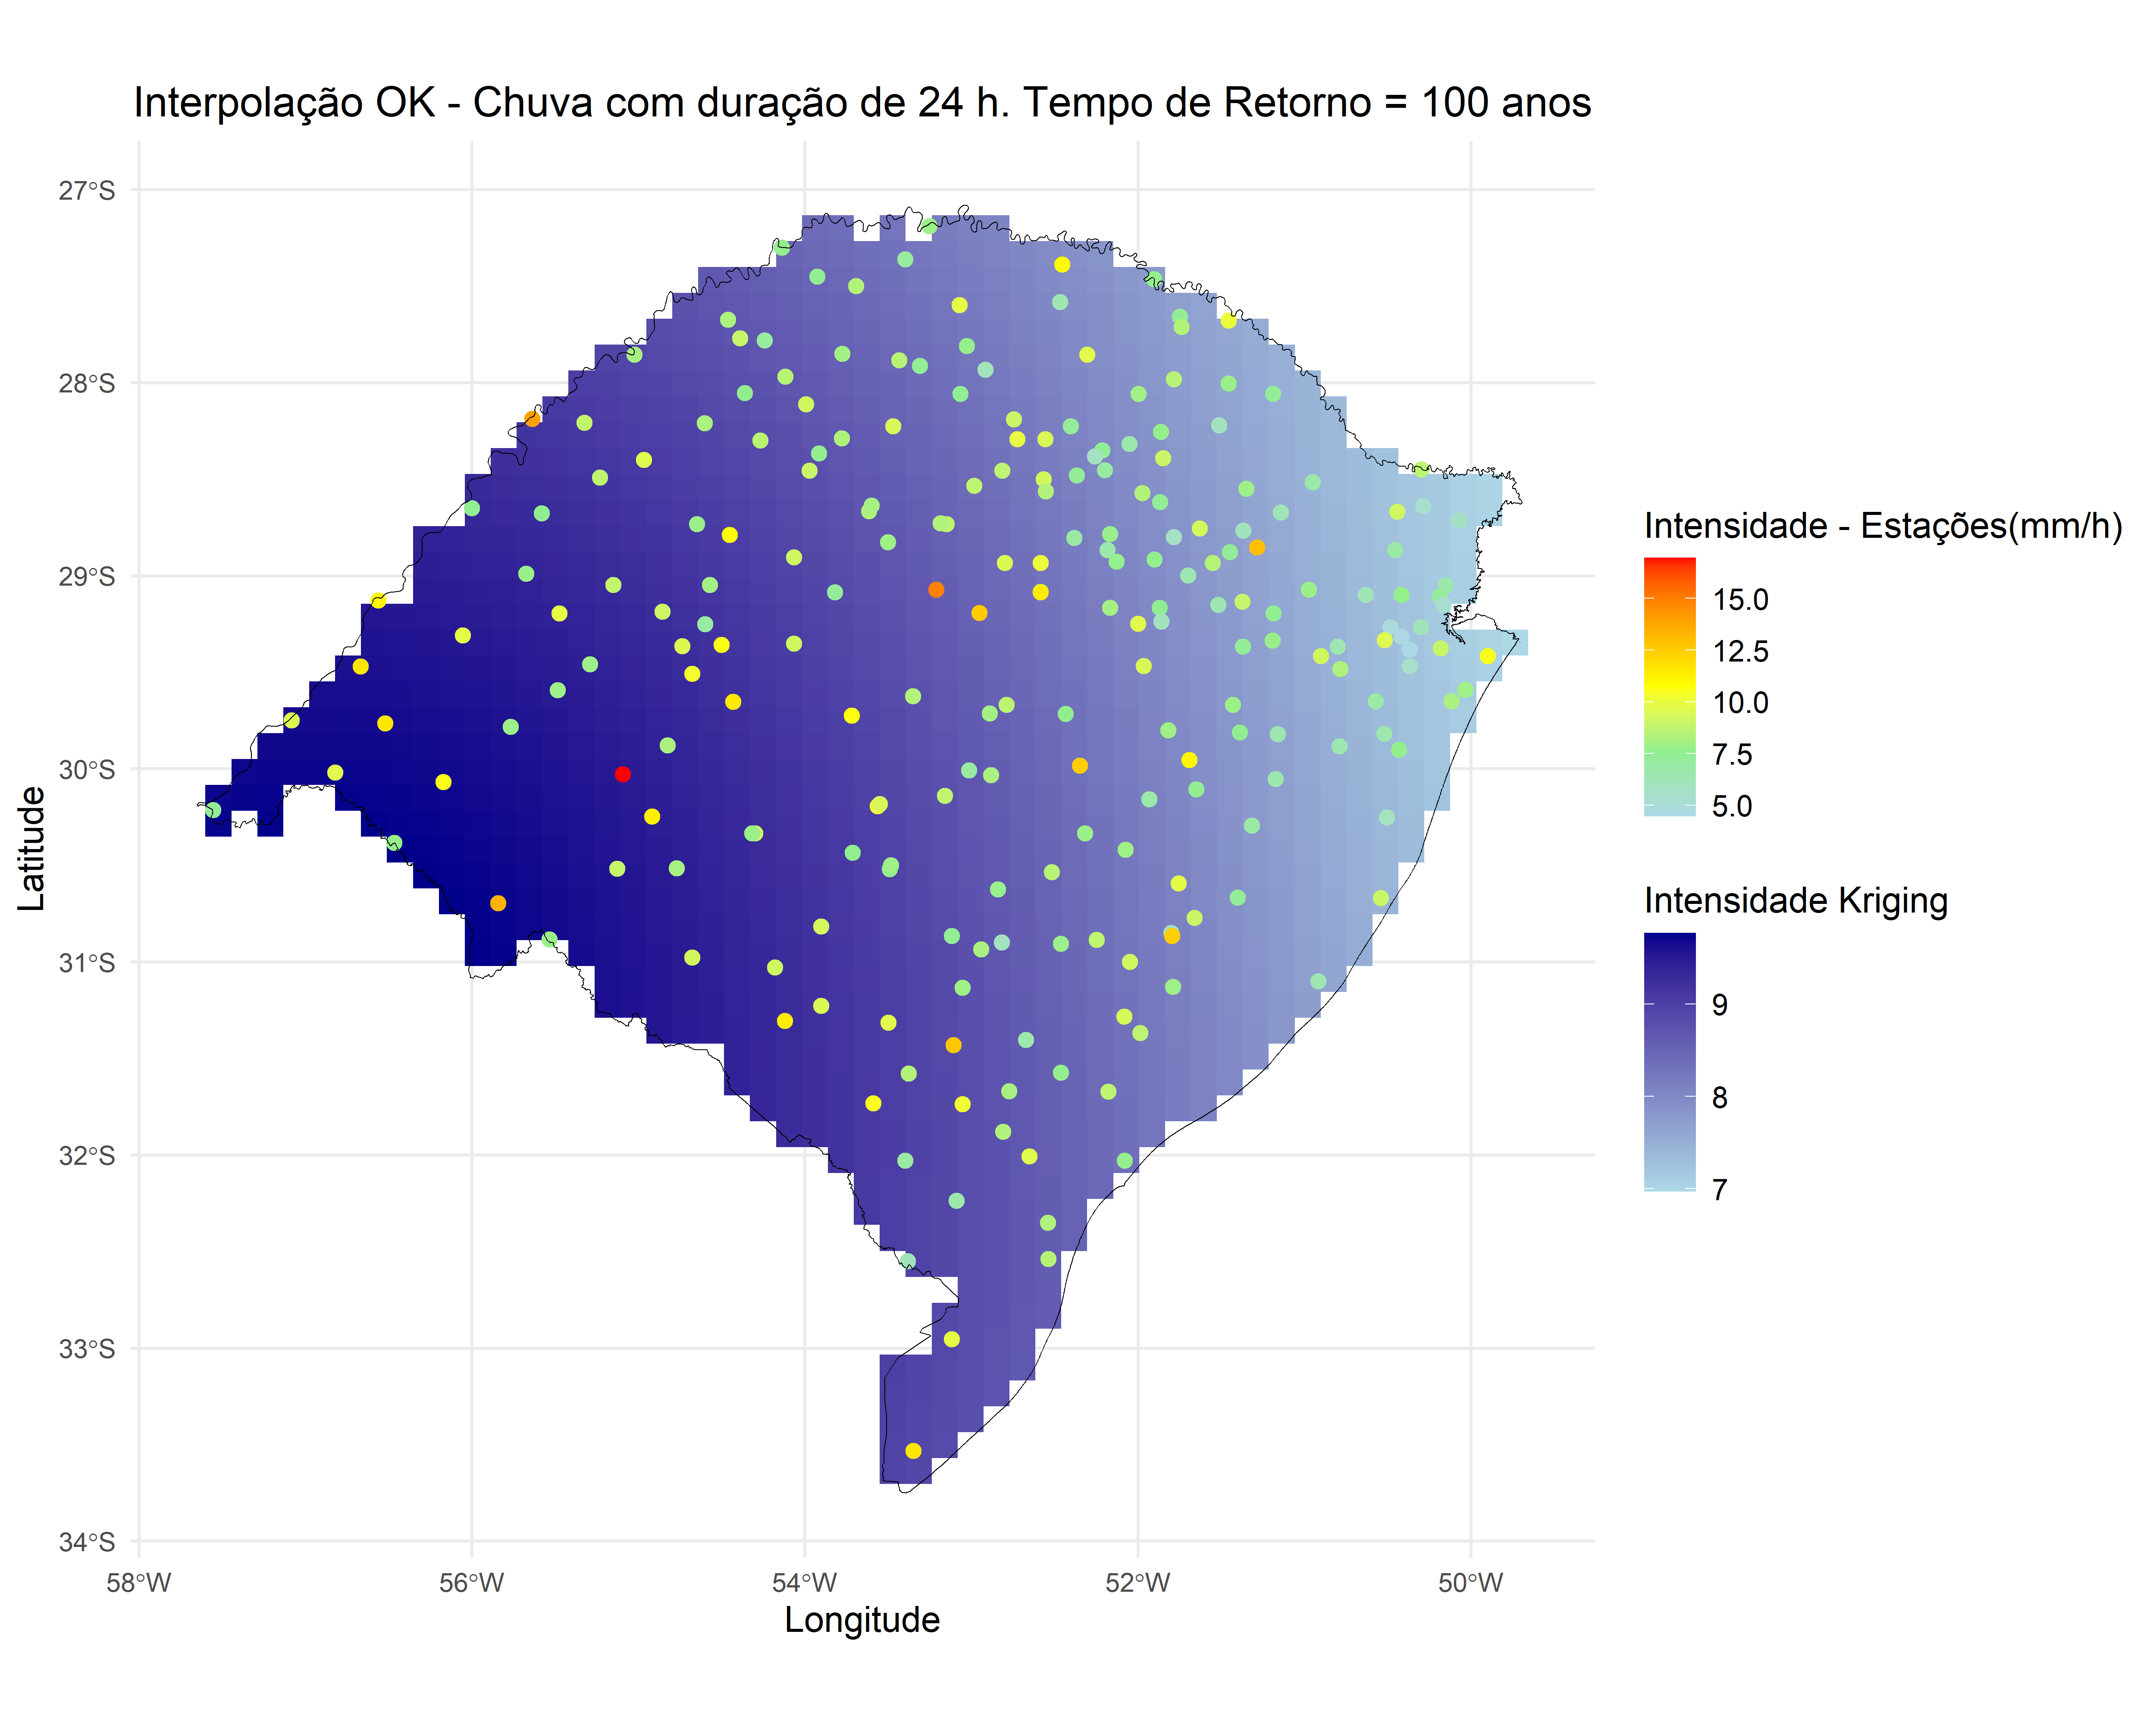
\includegraphics{Figuras/Figura13b.png}

}

\subcaption{\label{fig-Figura13b}Espacialização por OK. Tempo de Retorno
=100 anos}

\end{minipage}%
\newline
\begin{minipage}{\linewidth}
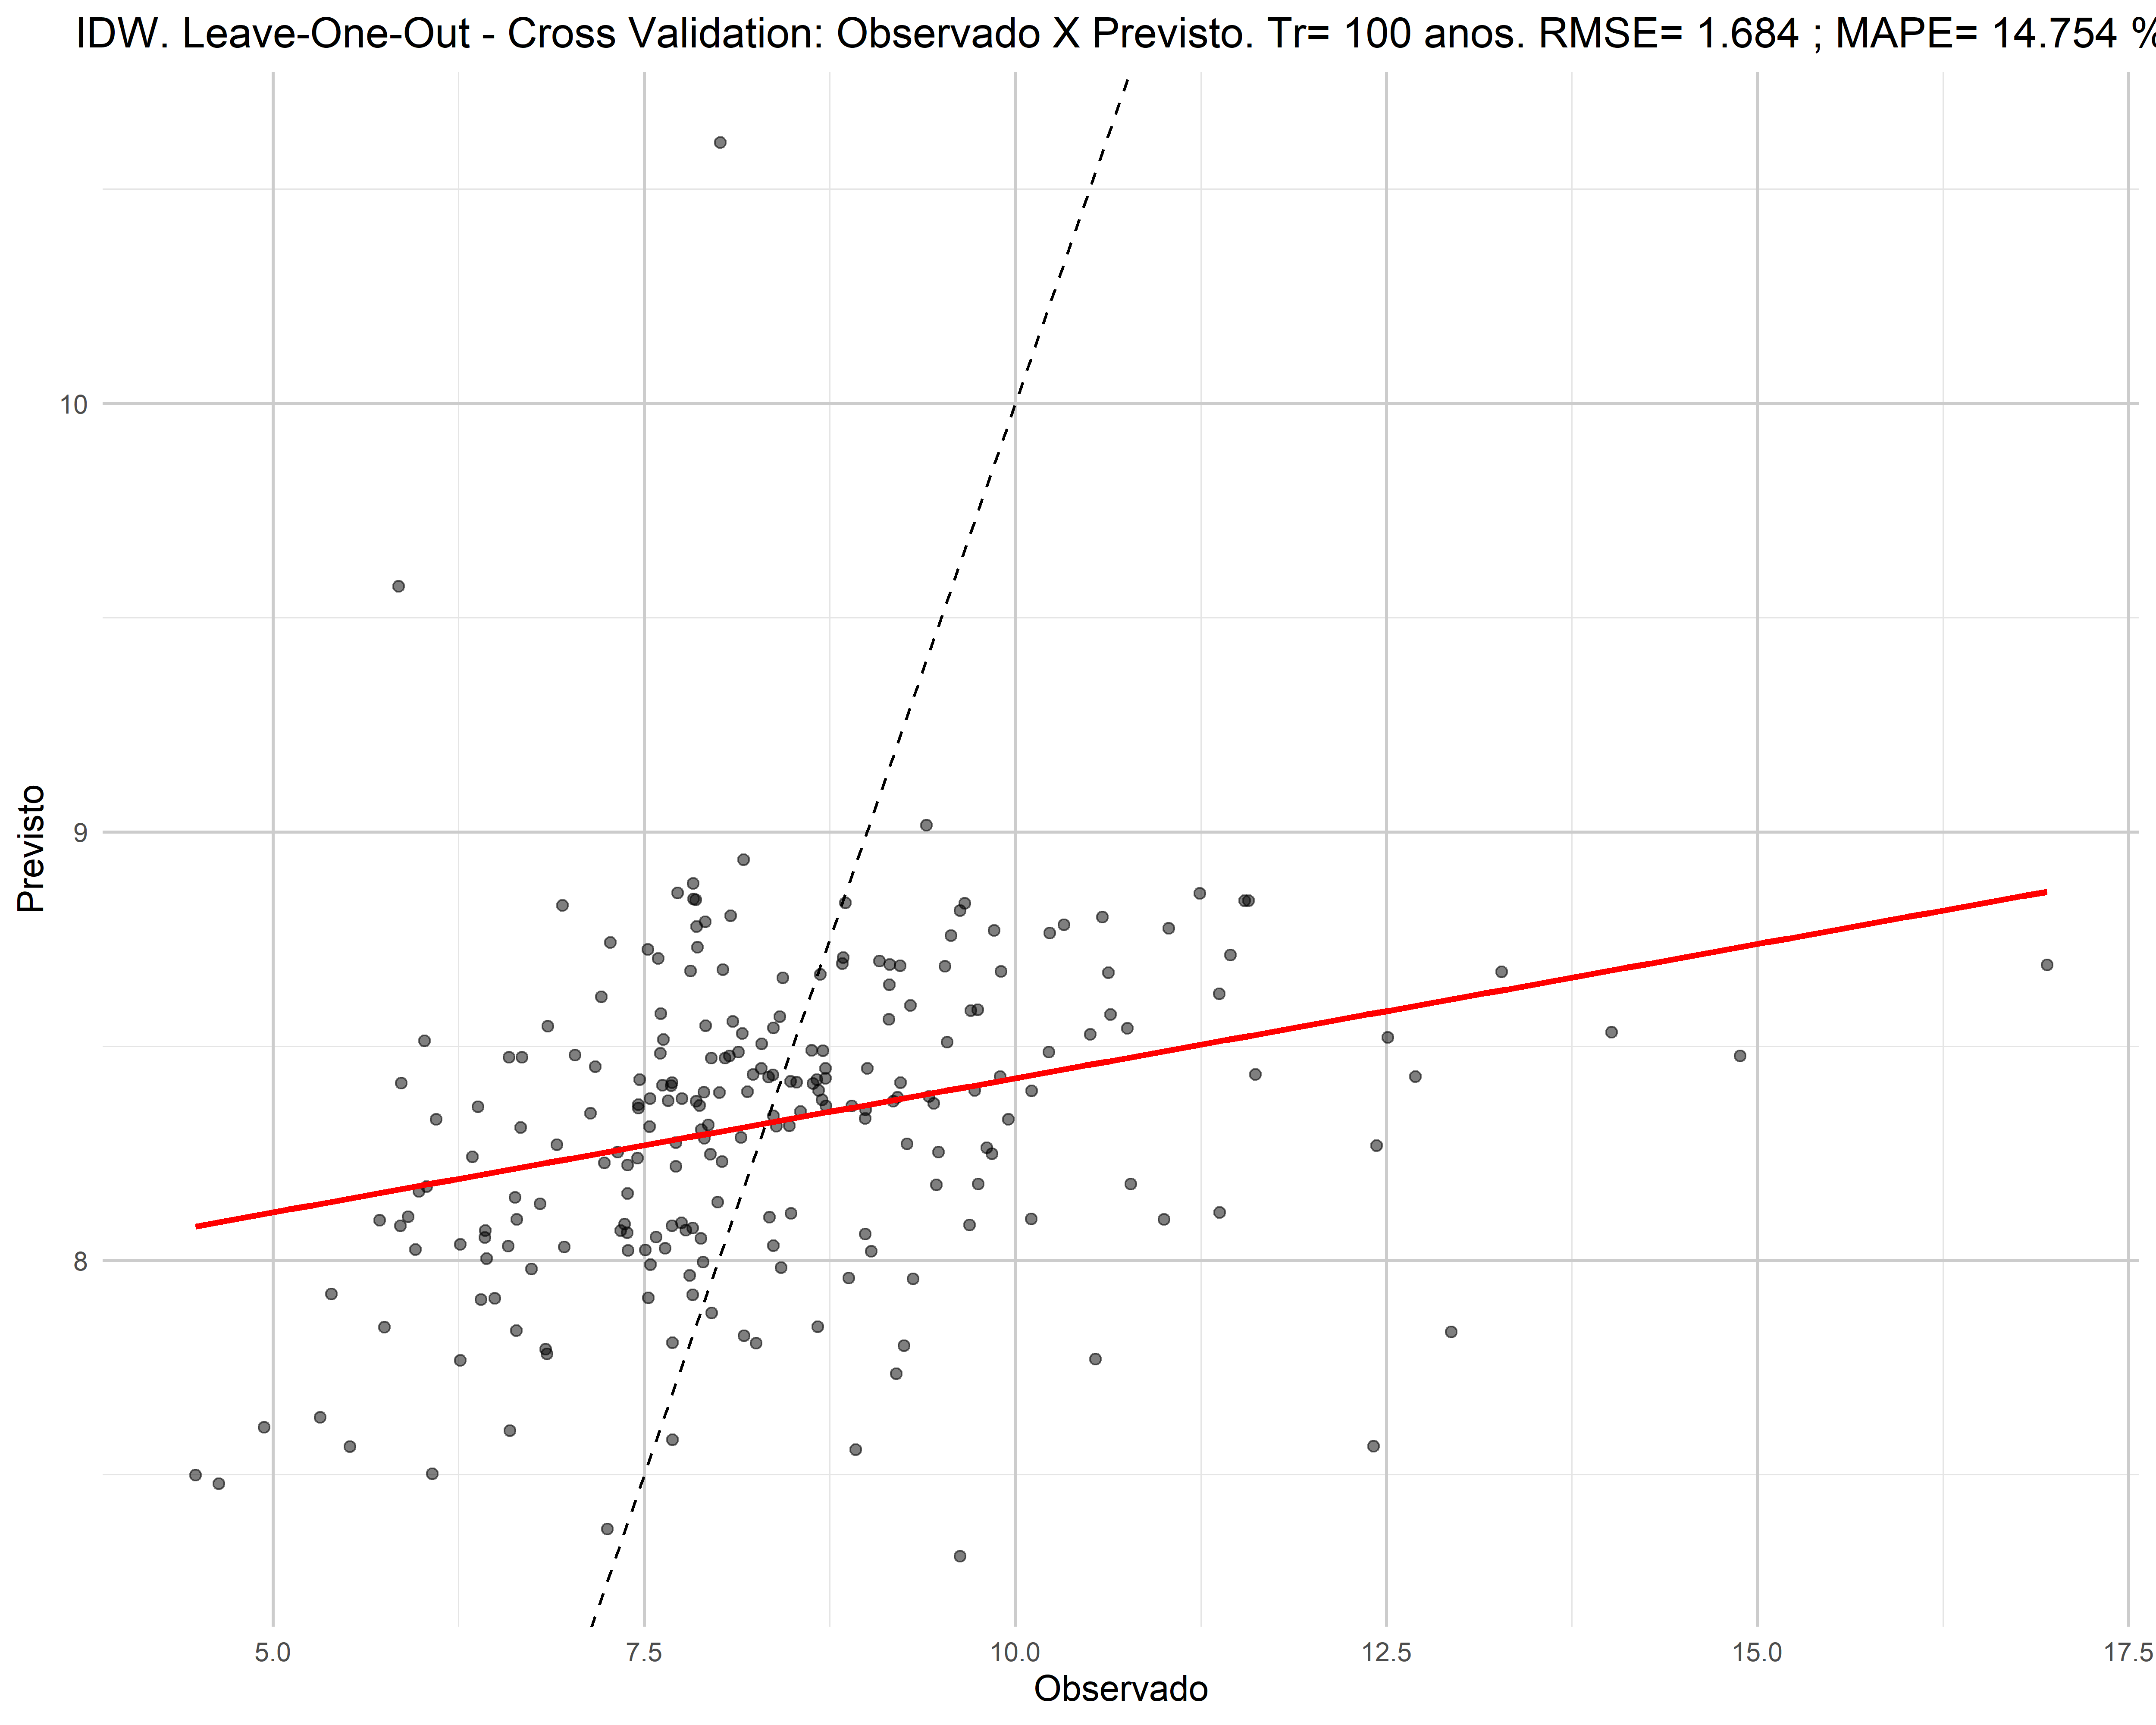
\includegraphics{Figuras/Figura13c.png}
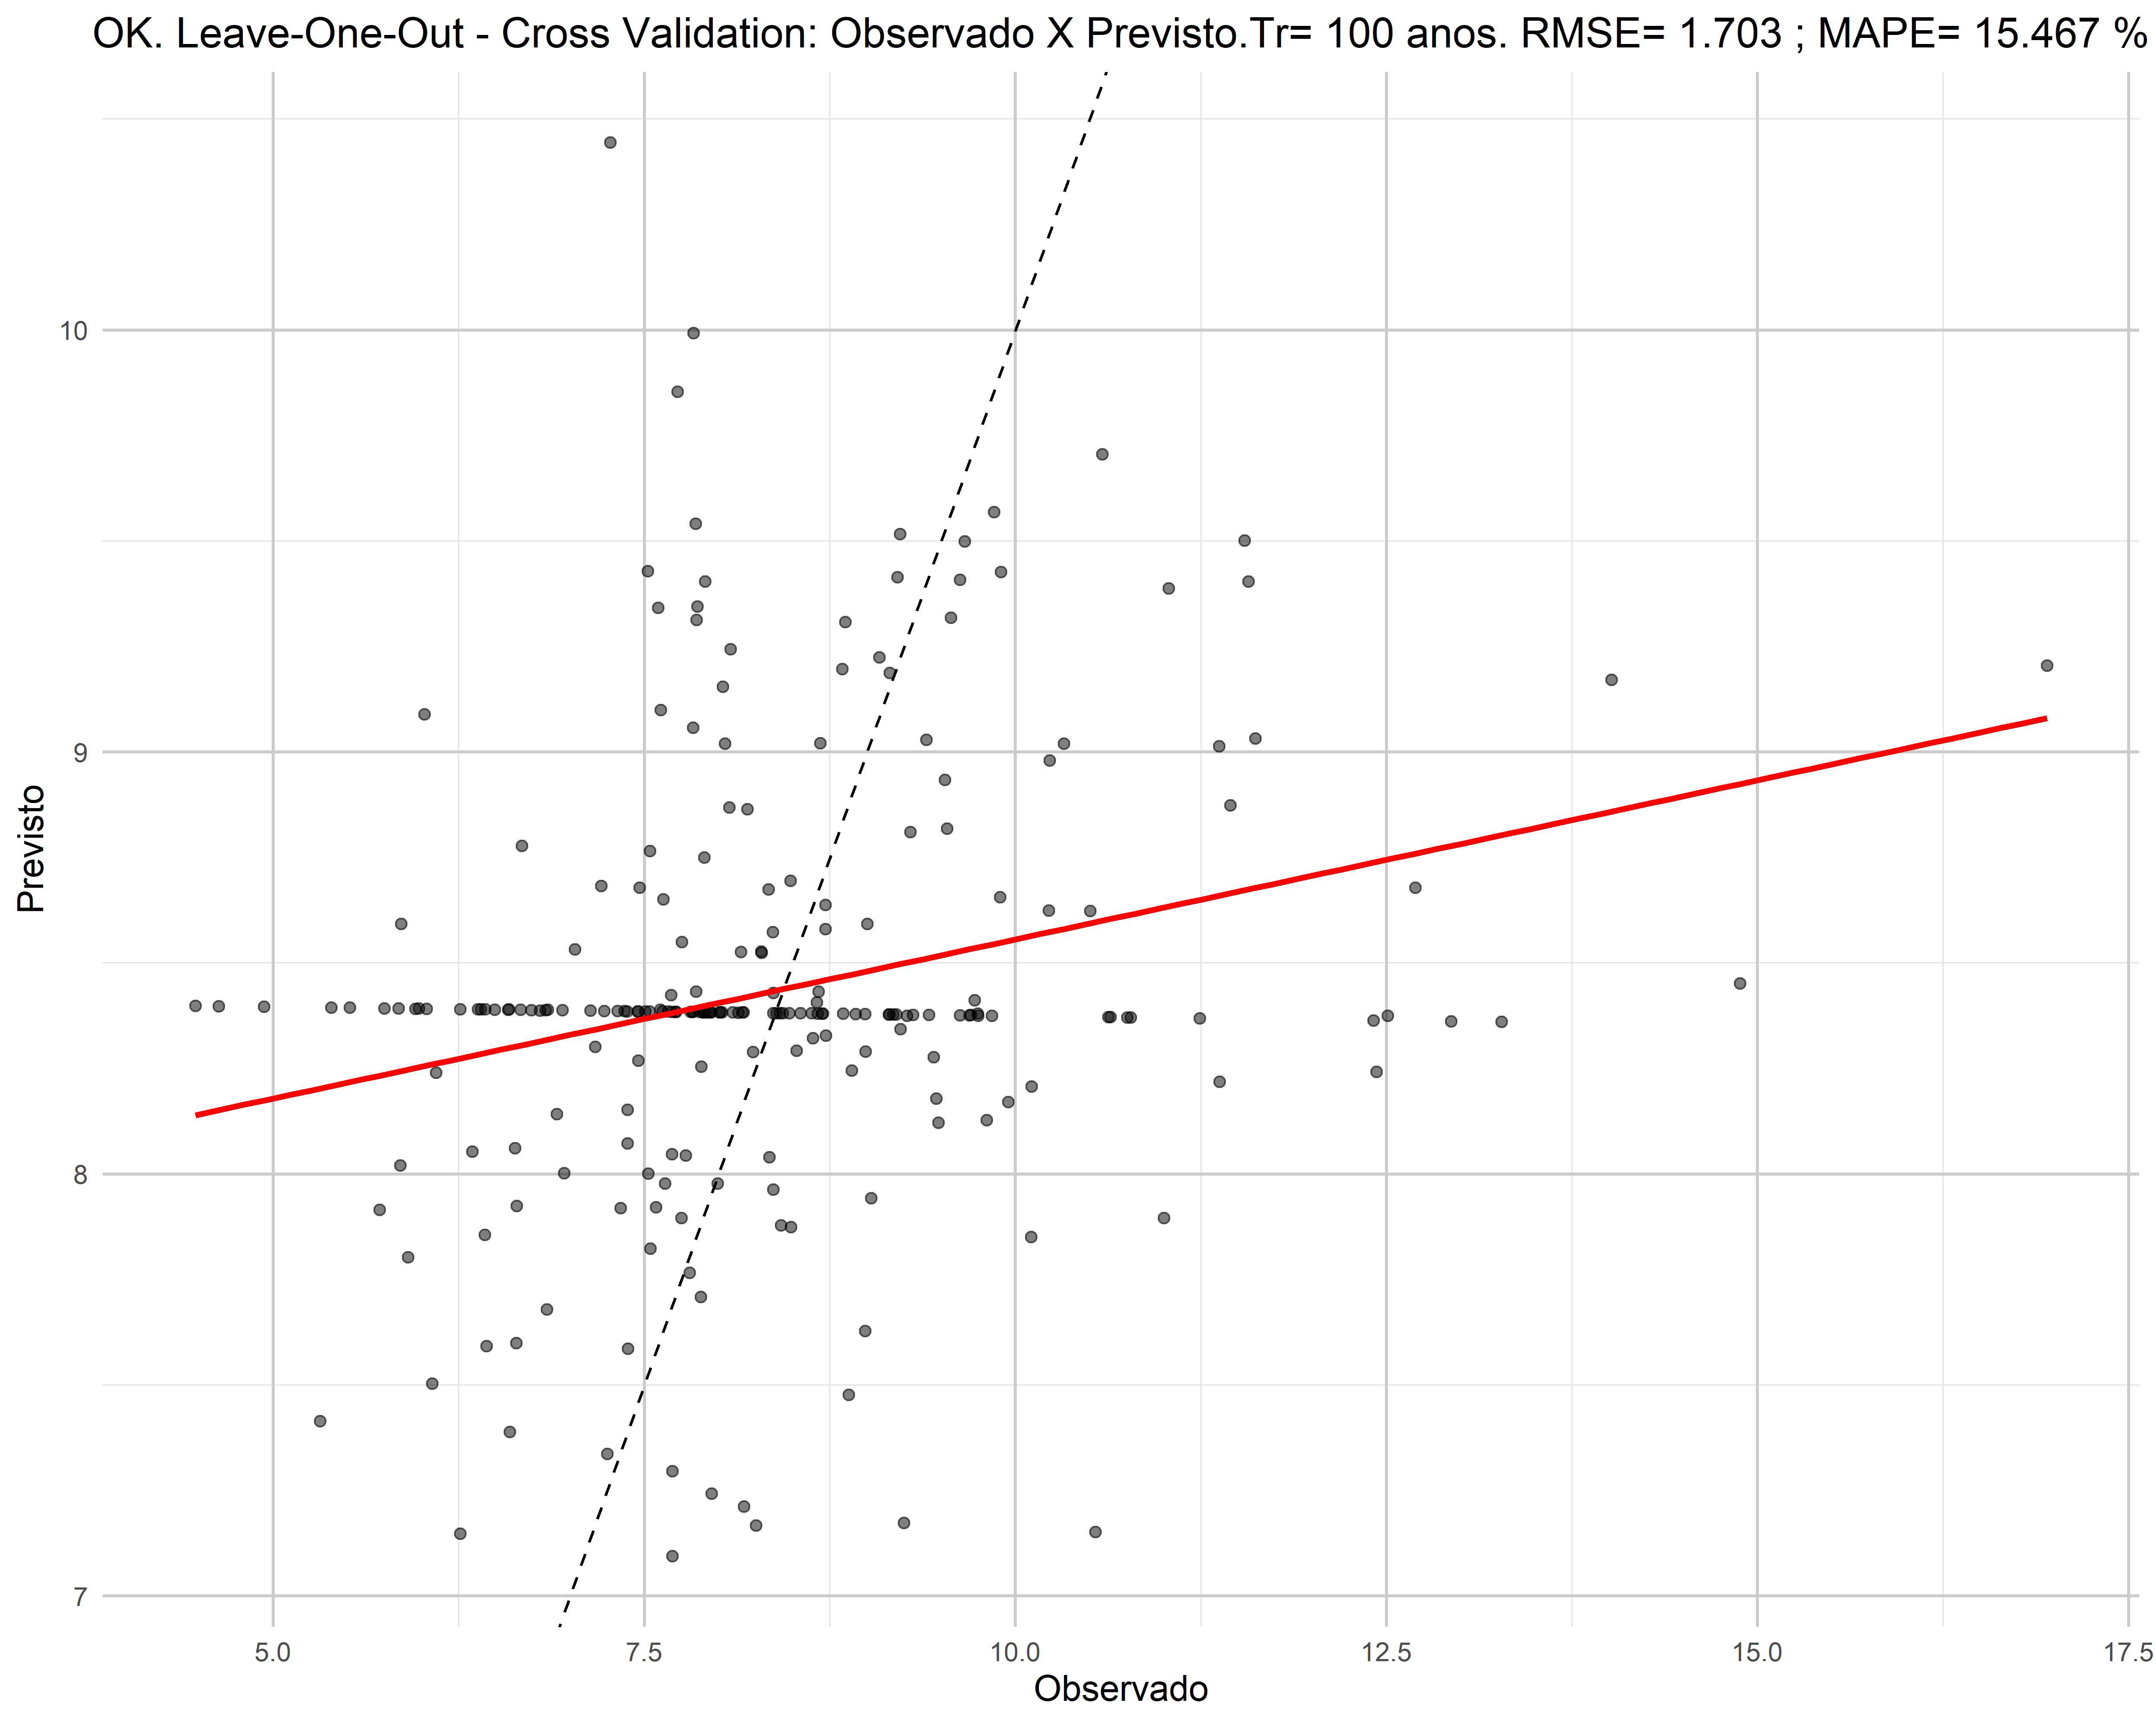
\includegraphics{Figuras/Figura13d.png}\end{minipage}%

\caption{\label{fig-Figura13}Resultados obtidos para intensidade da
chuva de duração de 24 h e tempo de retorno de 100 anos para
interpolação por IDW (a) e por krigagem ordinária, OK (b). Valores
preditos em função dos valores observados e resultados das métricas RMSE
e MAPE para interpolação por IDW (c) e OK (d).}

\end{figure}%

\begin{figure}

\begin{minipage}{\linewidth}

\centering{

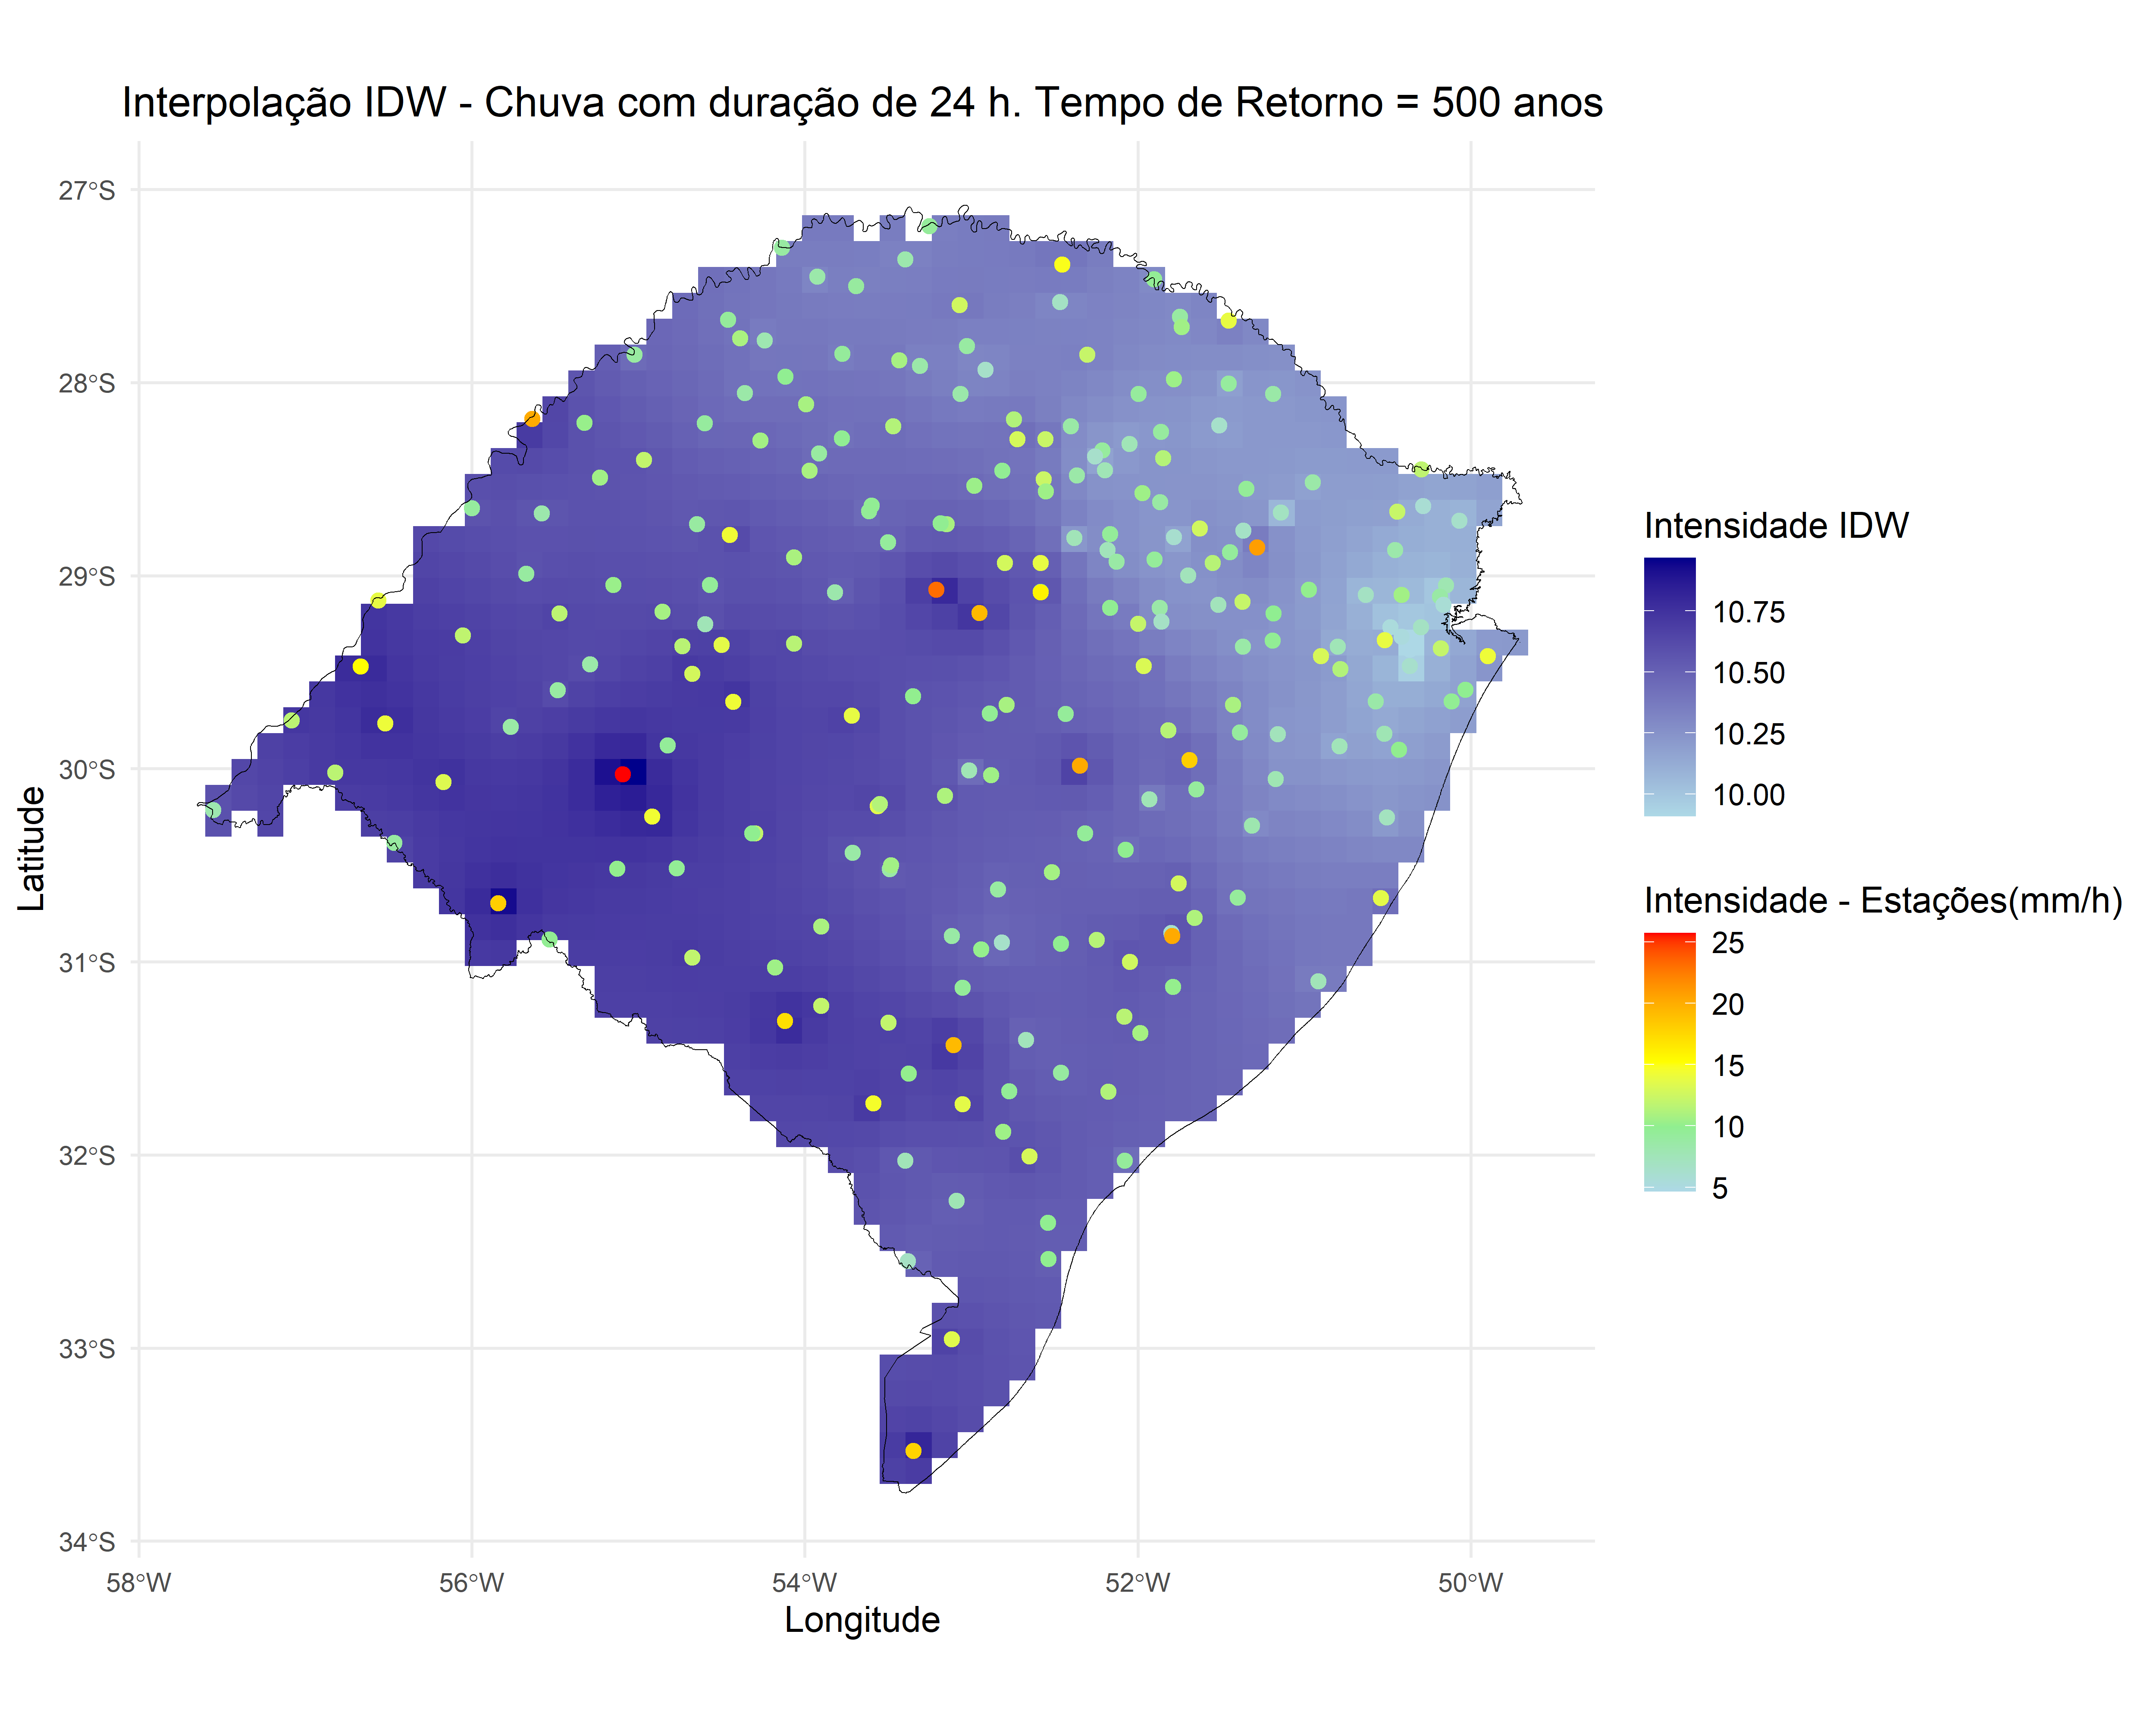
\includegraphics{Figuras/Figura14a.png}

}

\subcaption{\label{fig-Figura14a}Espacialização por IDW (p=1). Tempo de
Retorno =500 anos}

\end{minipage}%
\newline
\begin{minipage}{\linewidth}

\centering{

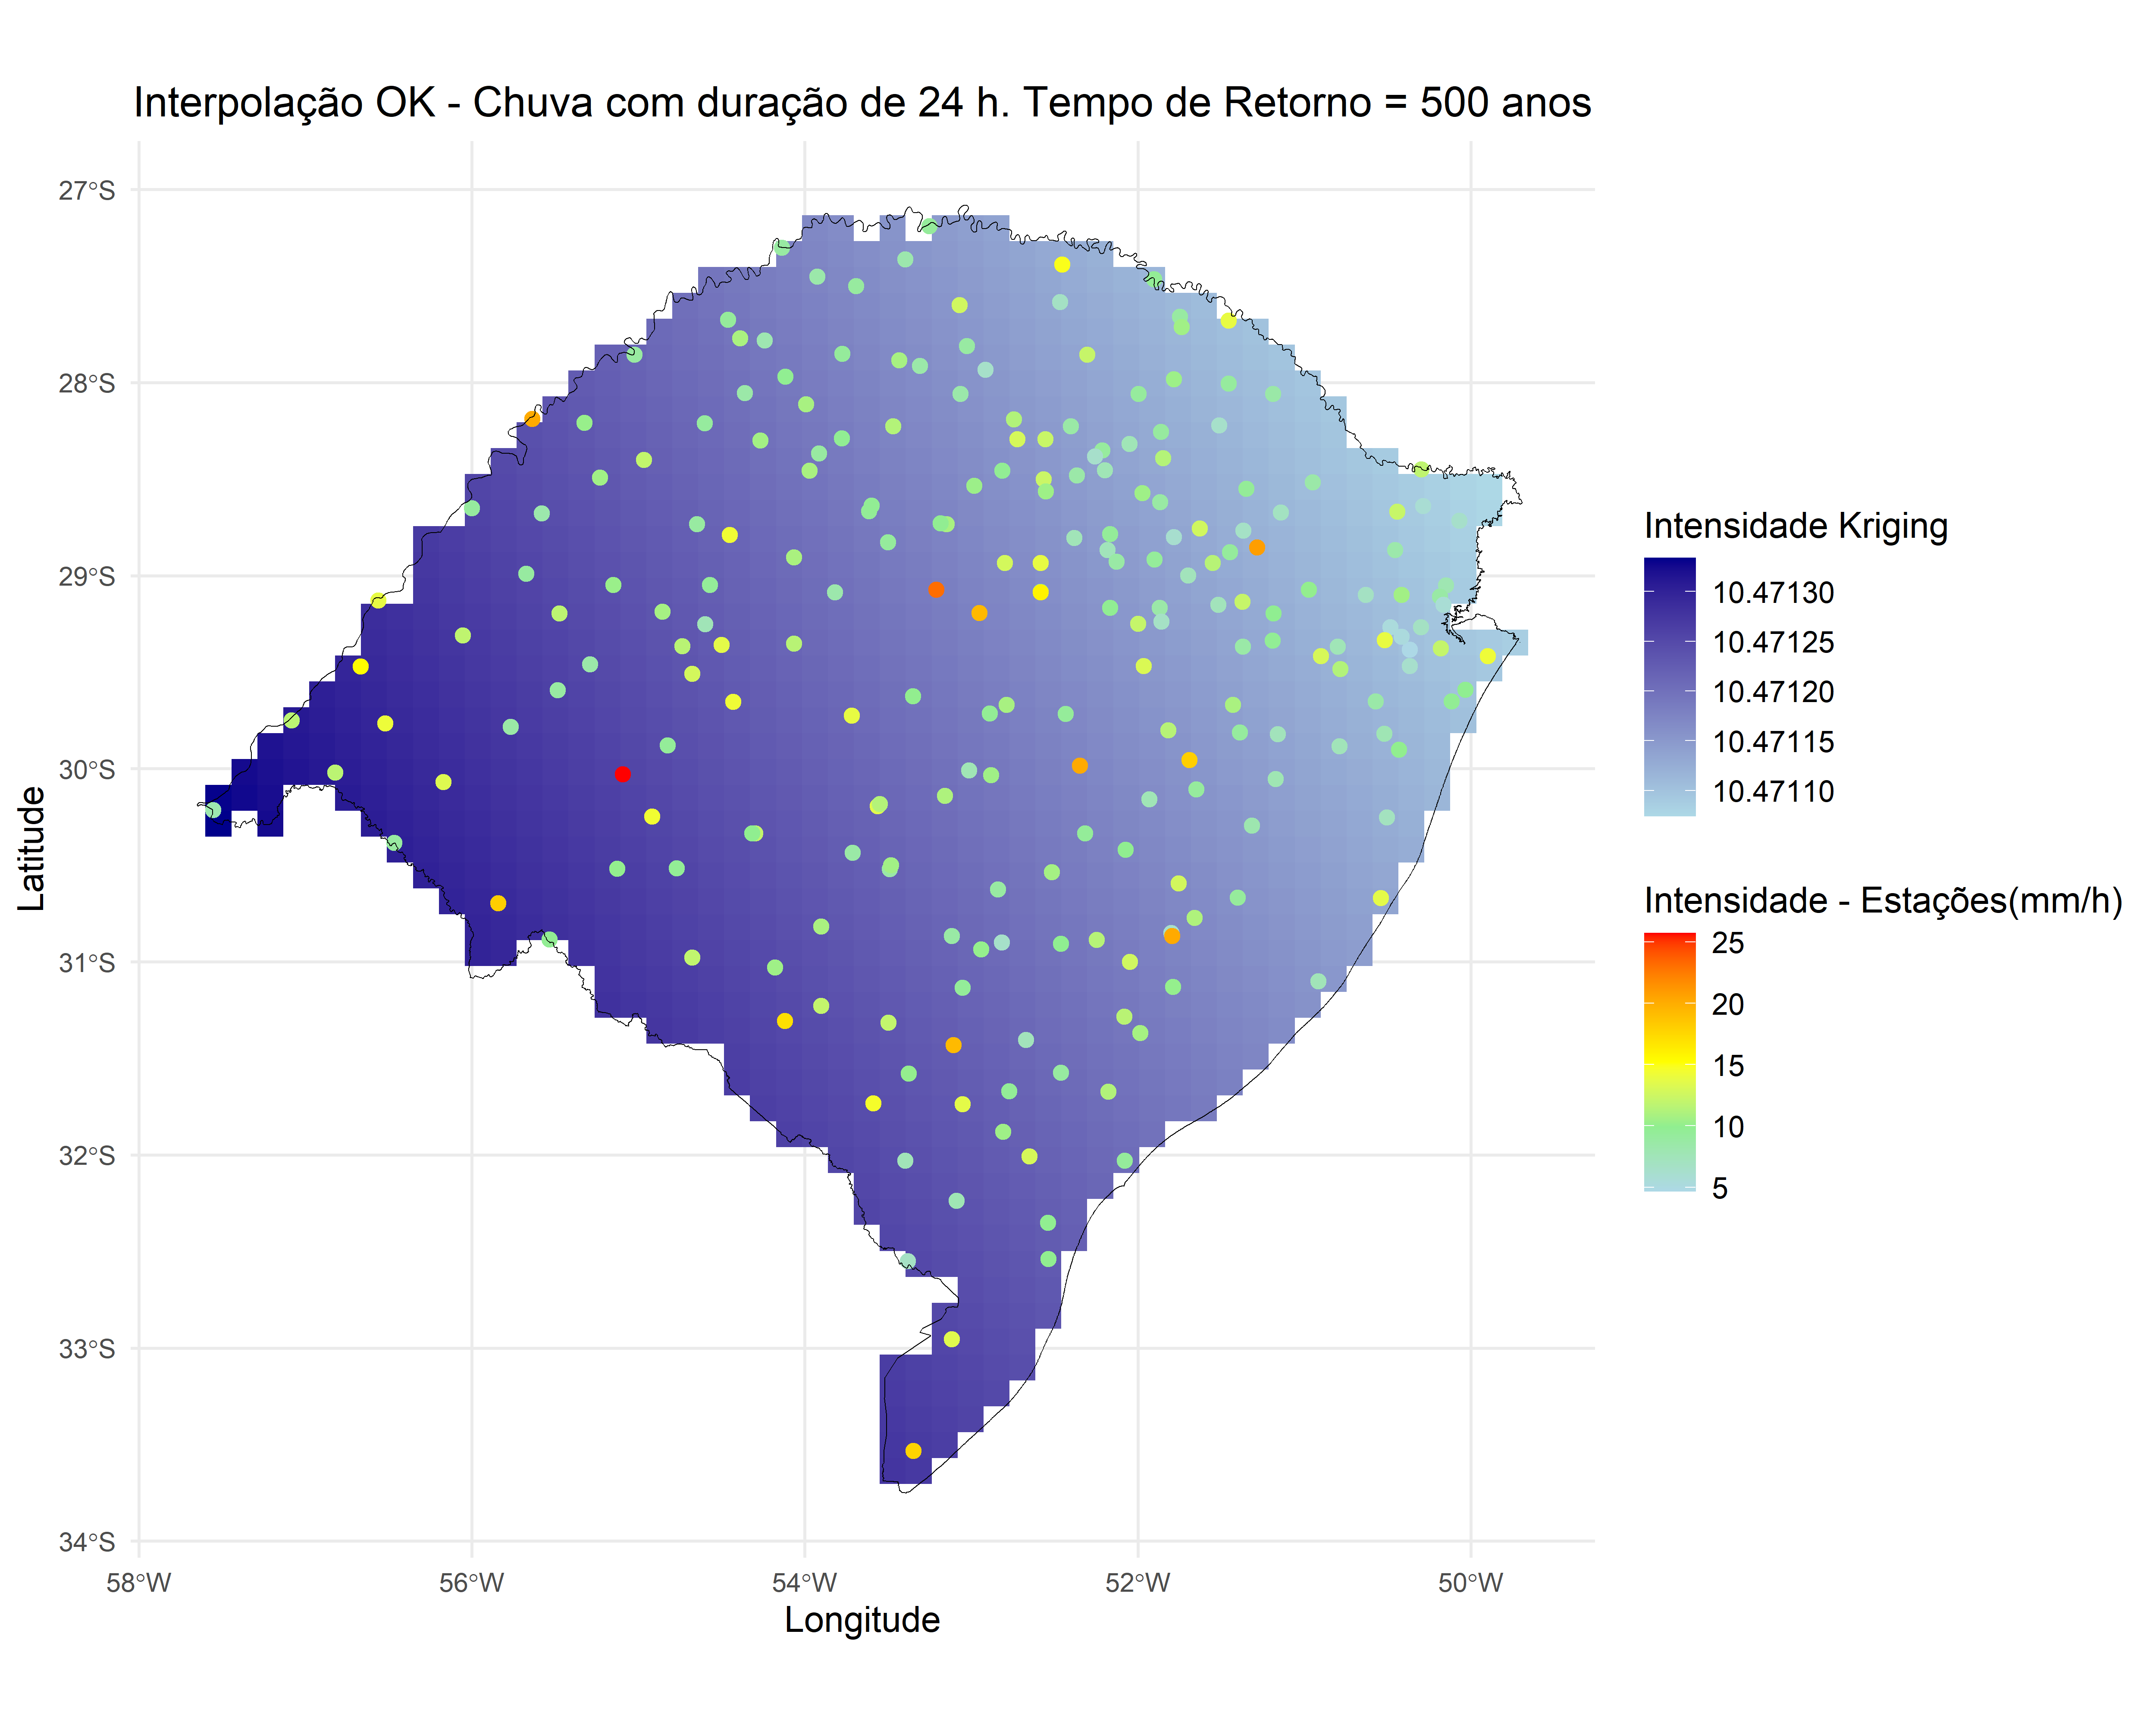
\includegraphics{Figuras/Figura14b.png}

}

\subcaption{\label{fig-Figura14b}Espacialização por OK. Tempo de Retorno
=500 anos}

\end{minipage}%
\newline
\begin{minipage}{\linewidth}
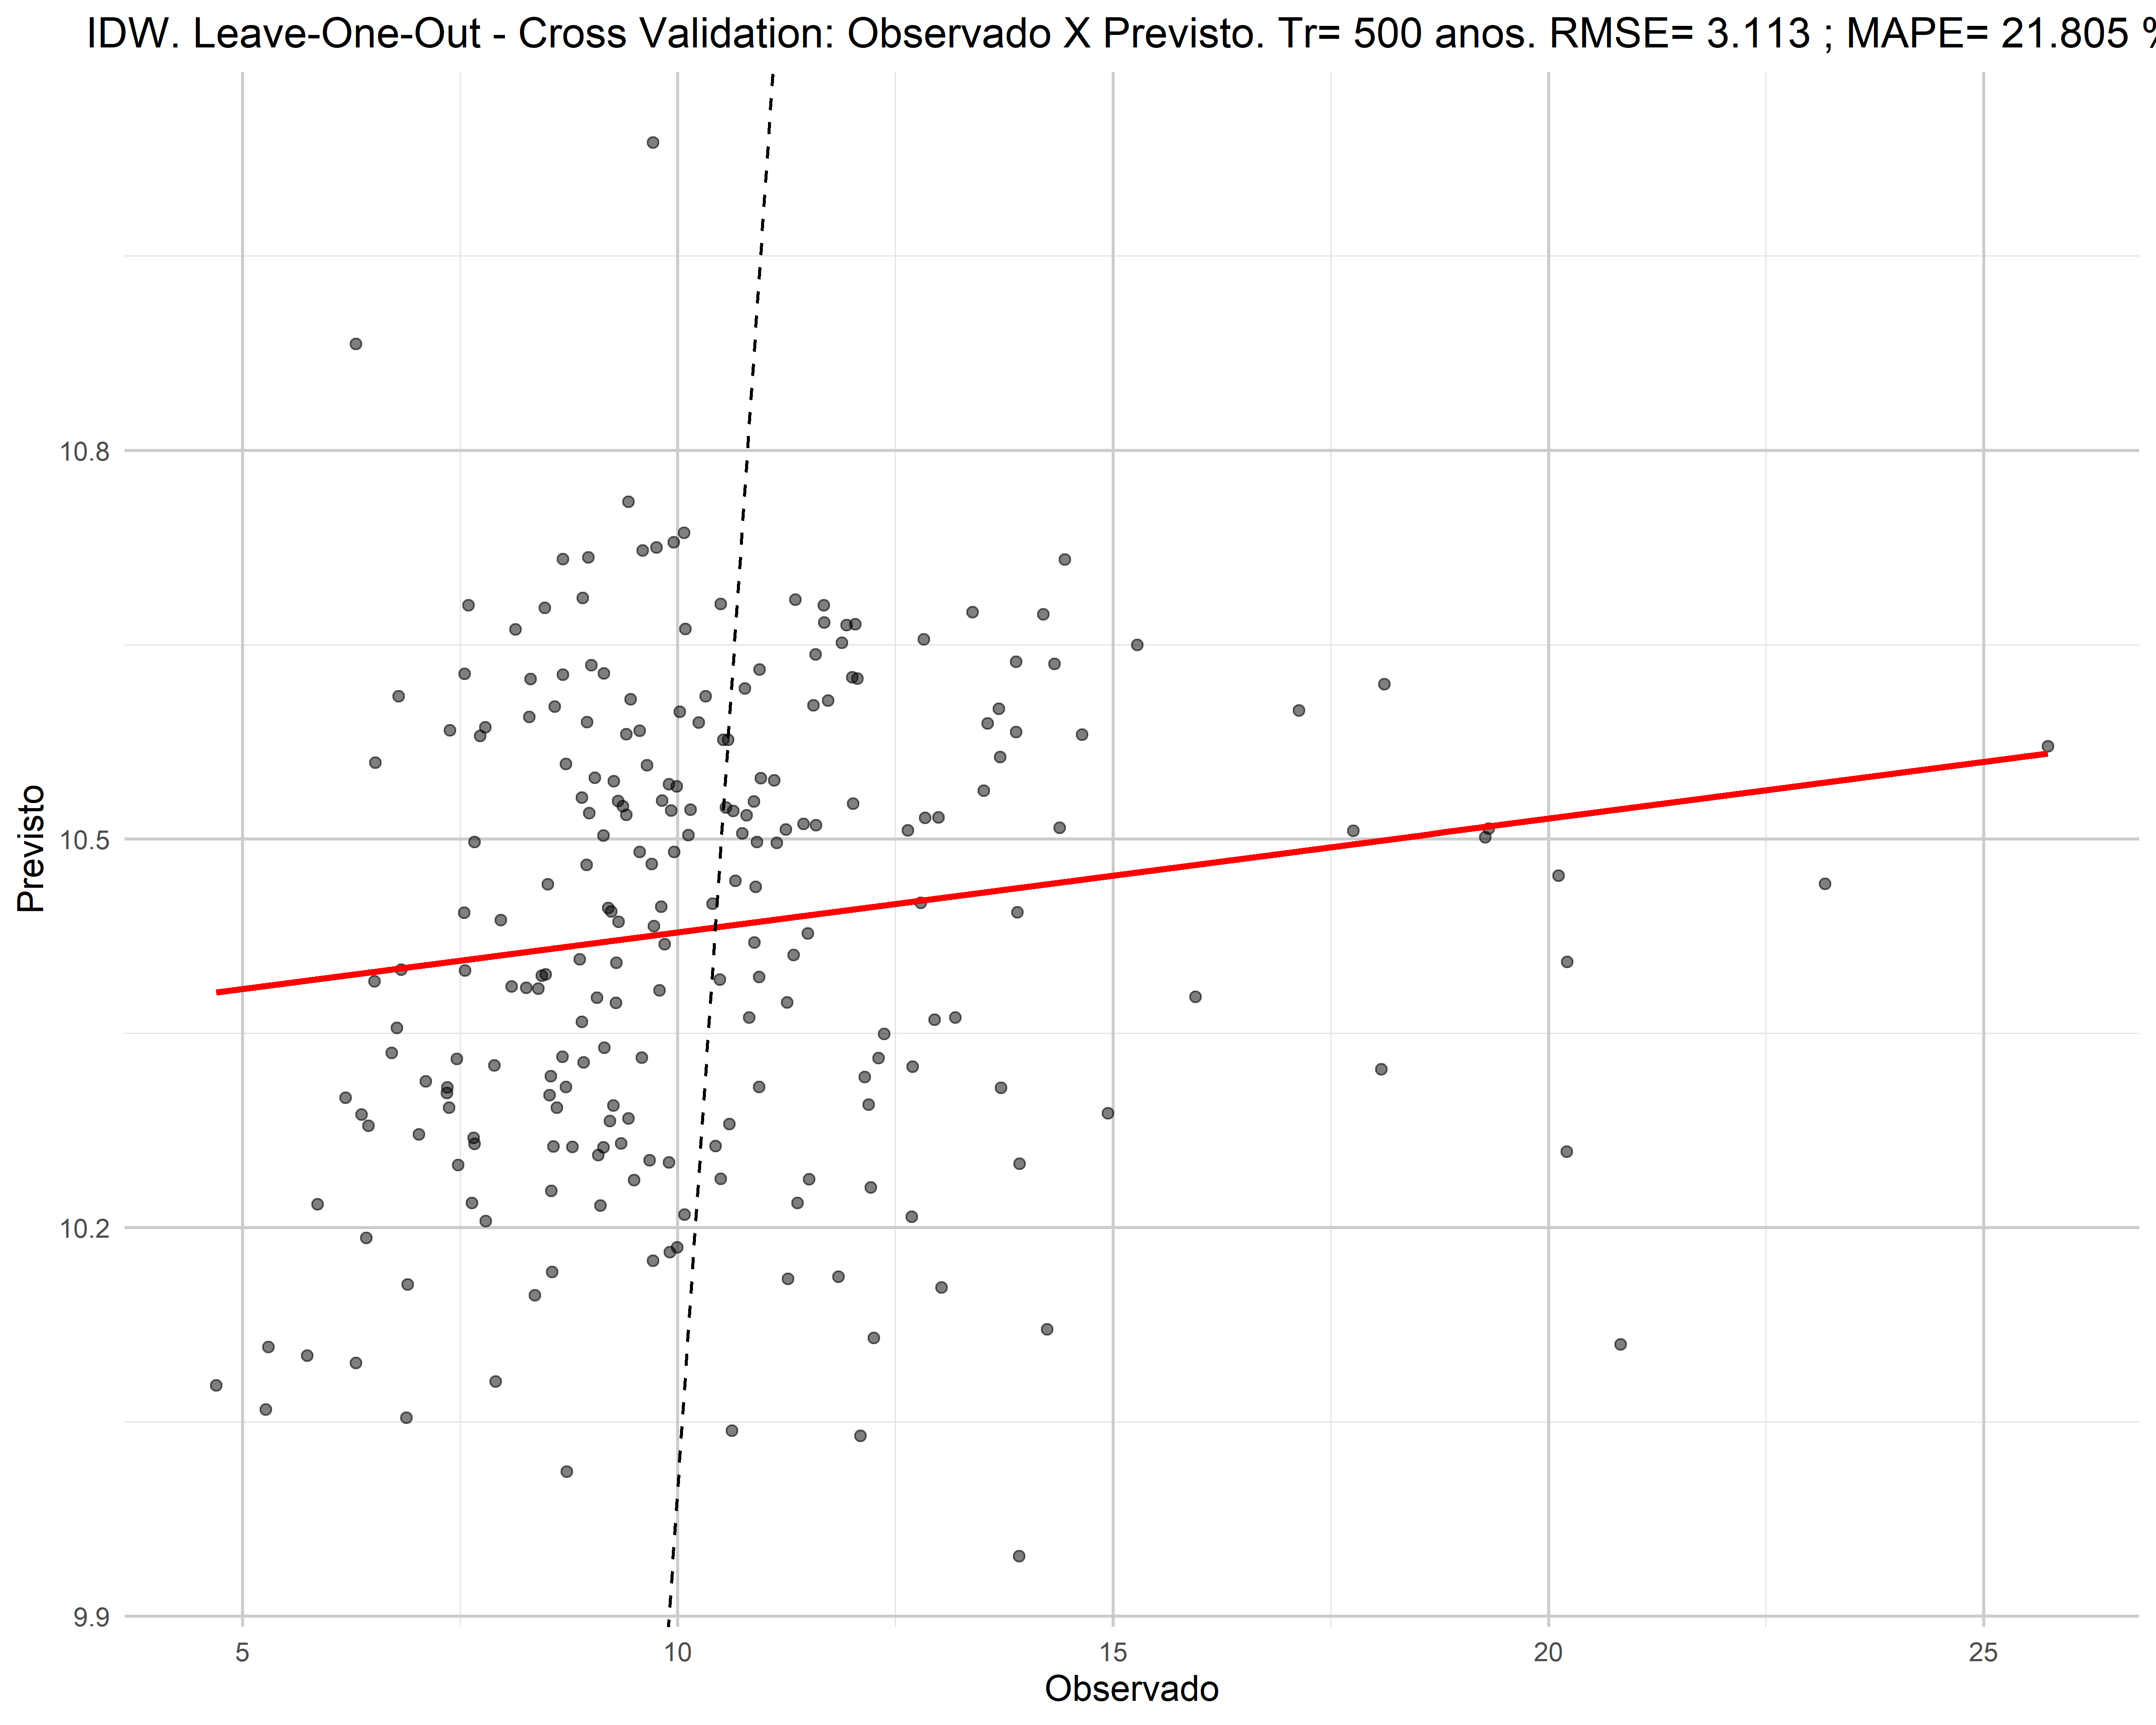
\includegraphics{Figuras/Figura14c.png}
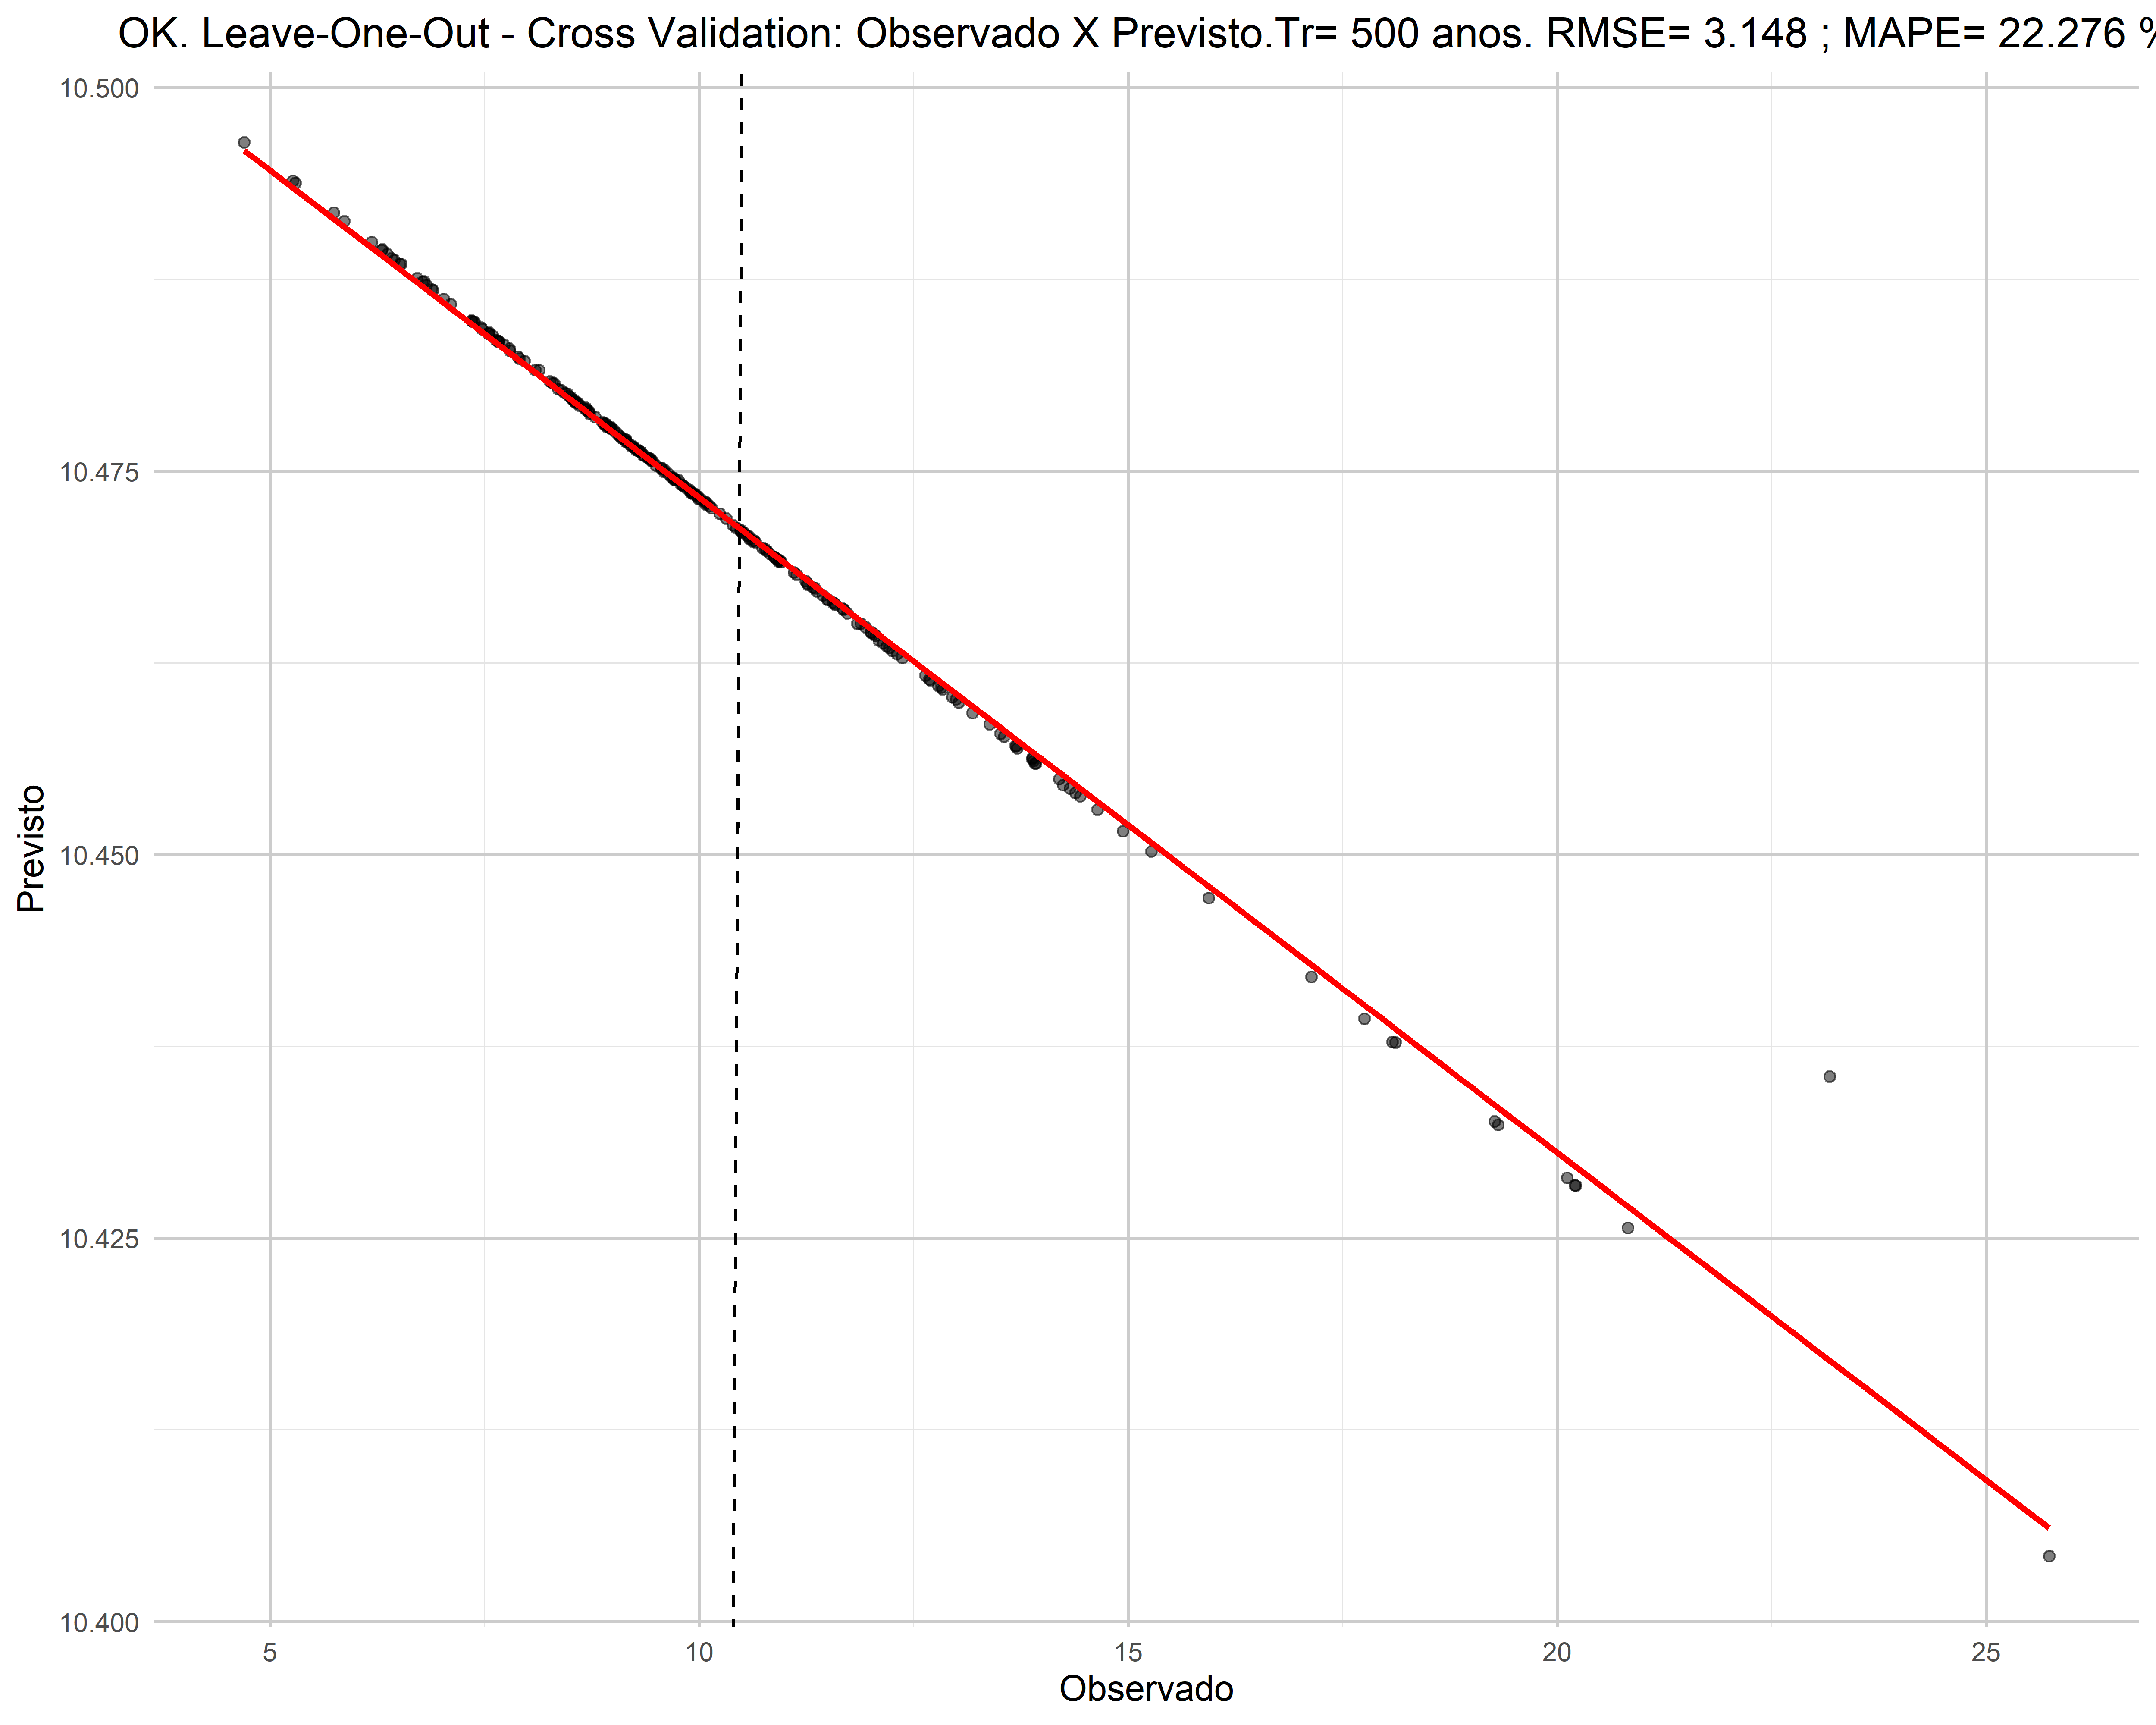
\includegraphics{Figuras/Figura14d.png}\end{minipage}%

\caption{\label{fig-Figura14}Resultados obtidos para intensidade da
chuva de duração de 24 h e tempo de retorno de 500 anos para
interpolação por IDW (a) e por krigagem ordinária, OK (b). Valores
preditos em função dos valores observados e resultados das métricas RMSE
e MAPE para interpolação por IDW (c) e OK (d).}

\end{figure}%

A Figure~\ref{fig-Figura15a} e Figure~\ref{fig-Figura15b} mostram a
performance das métricas \(RMSE\) e \(MAPE\), respectivamente, para
ambos os modelos de interpolação adotados (IDW e Krigagem), considerando
diferentes tempos de retorno. Observa-se que, para tempos de retorno
menores, a interpolação por IDW apresenta desempenho ligeiramente
superior em relação às métricas avaliadas. No entanto, para tempos de
retorno maiores, a Krigagem tende a superar a interpolação por IDW.

Embora esses resultados sugiram que a escolha do método de interpolação
pode variar com o tempo de retorno, é importante considerar os
princípios e objetivos subjacentes a cada método, bem como as
características das variáveis ou fenômenos a serem interpolados. Como
descrito na metodologia, a Krigagem é particularmente adequada para
dados que apresentam padrões de autocorrelação espacial. No contexto dos
dados de chuvas extremas, que são coletados por várias estações
distribuídas espacialmente, a construção das curvas IDFs em cada estação
é baseada em séries históricas de máximos diários anuais de
precipitação. No entanto, os eventos máximos registrados em uma estação
não estão necessariamente correlacionados com os eventos máximos
registrados em outras estações. Em outras palavras, a chuva máxima
observada no histórico anual de uma estação não precisa corresponder ao
mesmo evento de chuva que gerou o valor máximo anual em outra estação.
Contudo, certamente, entre estações muito próximas pode haver registros
de chuvas máximas que foram oriundas do mesmo evento, ou, ainda, mesmo
para eventos de chuvas máximas independentes, pode existir correlação
devido a outros padrões de sistemas meteorológicos que podem afetar
áreas adjacentes simultaneamente. Este campo permanece aberto para
pesquisas e o aprimoramento de técnicas de regionalização que visem
reduzir as incertezas associadas à espacialização das curvas IDFs.

\begin{figure}

\begin{minipage}{\linewidth}

\centering{

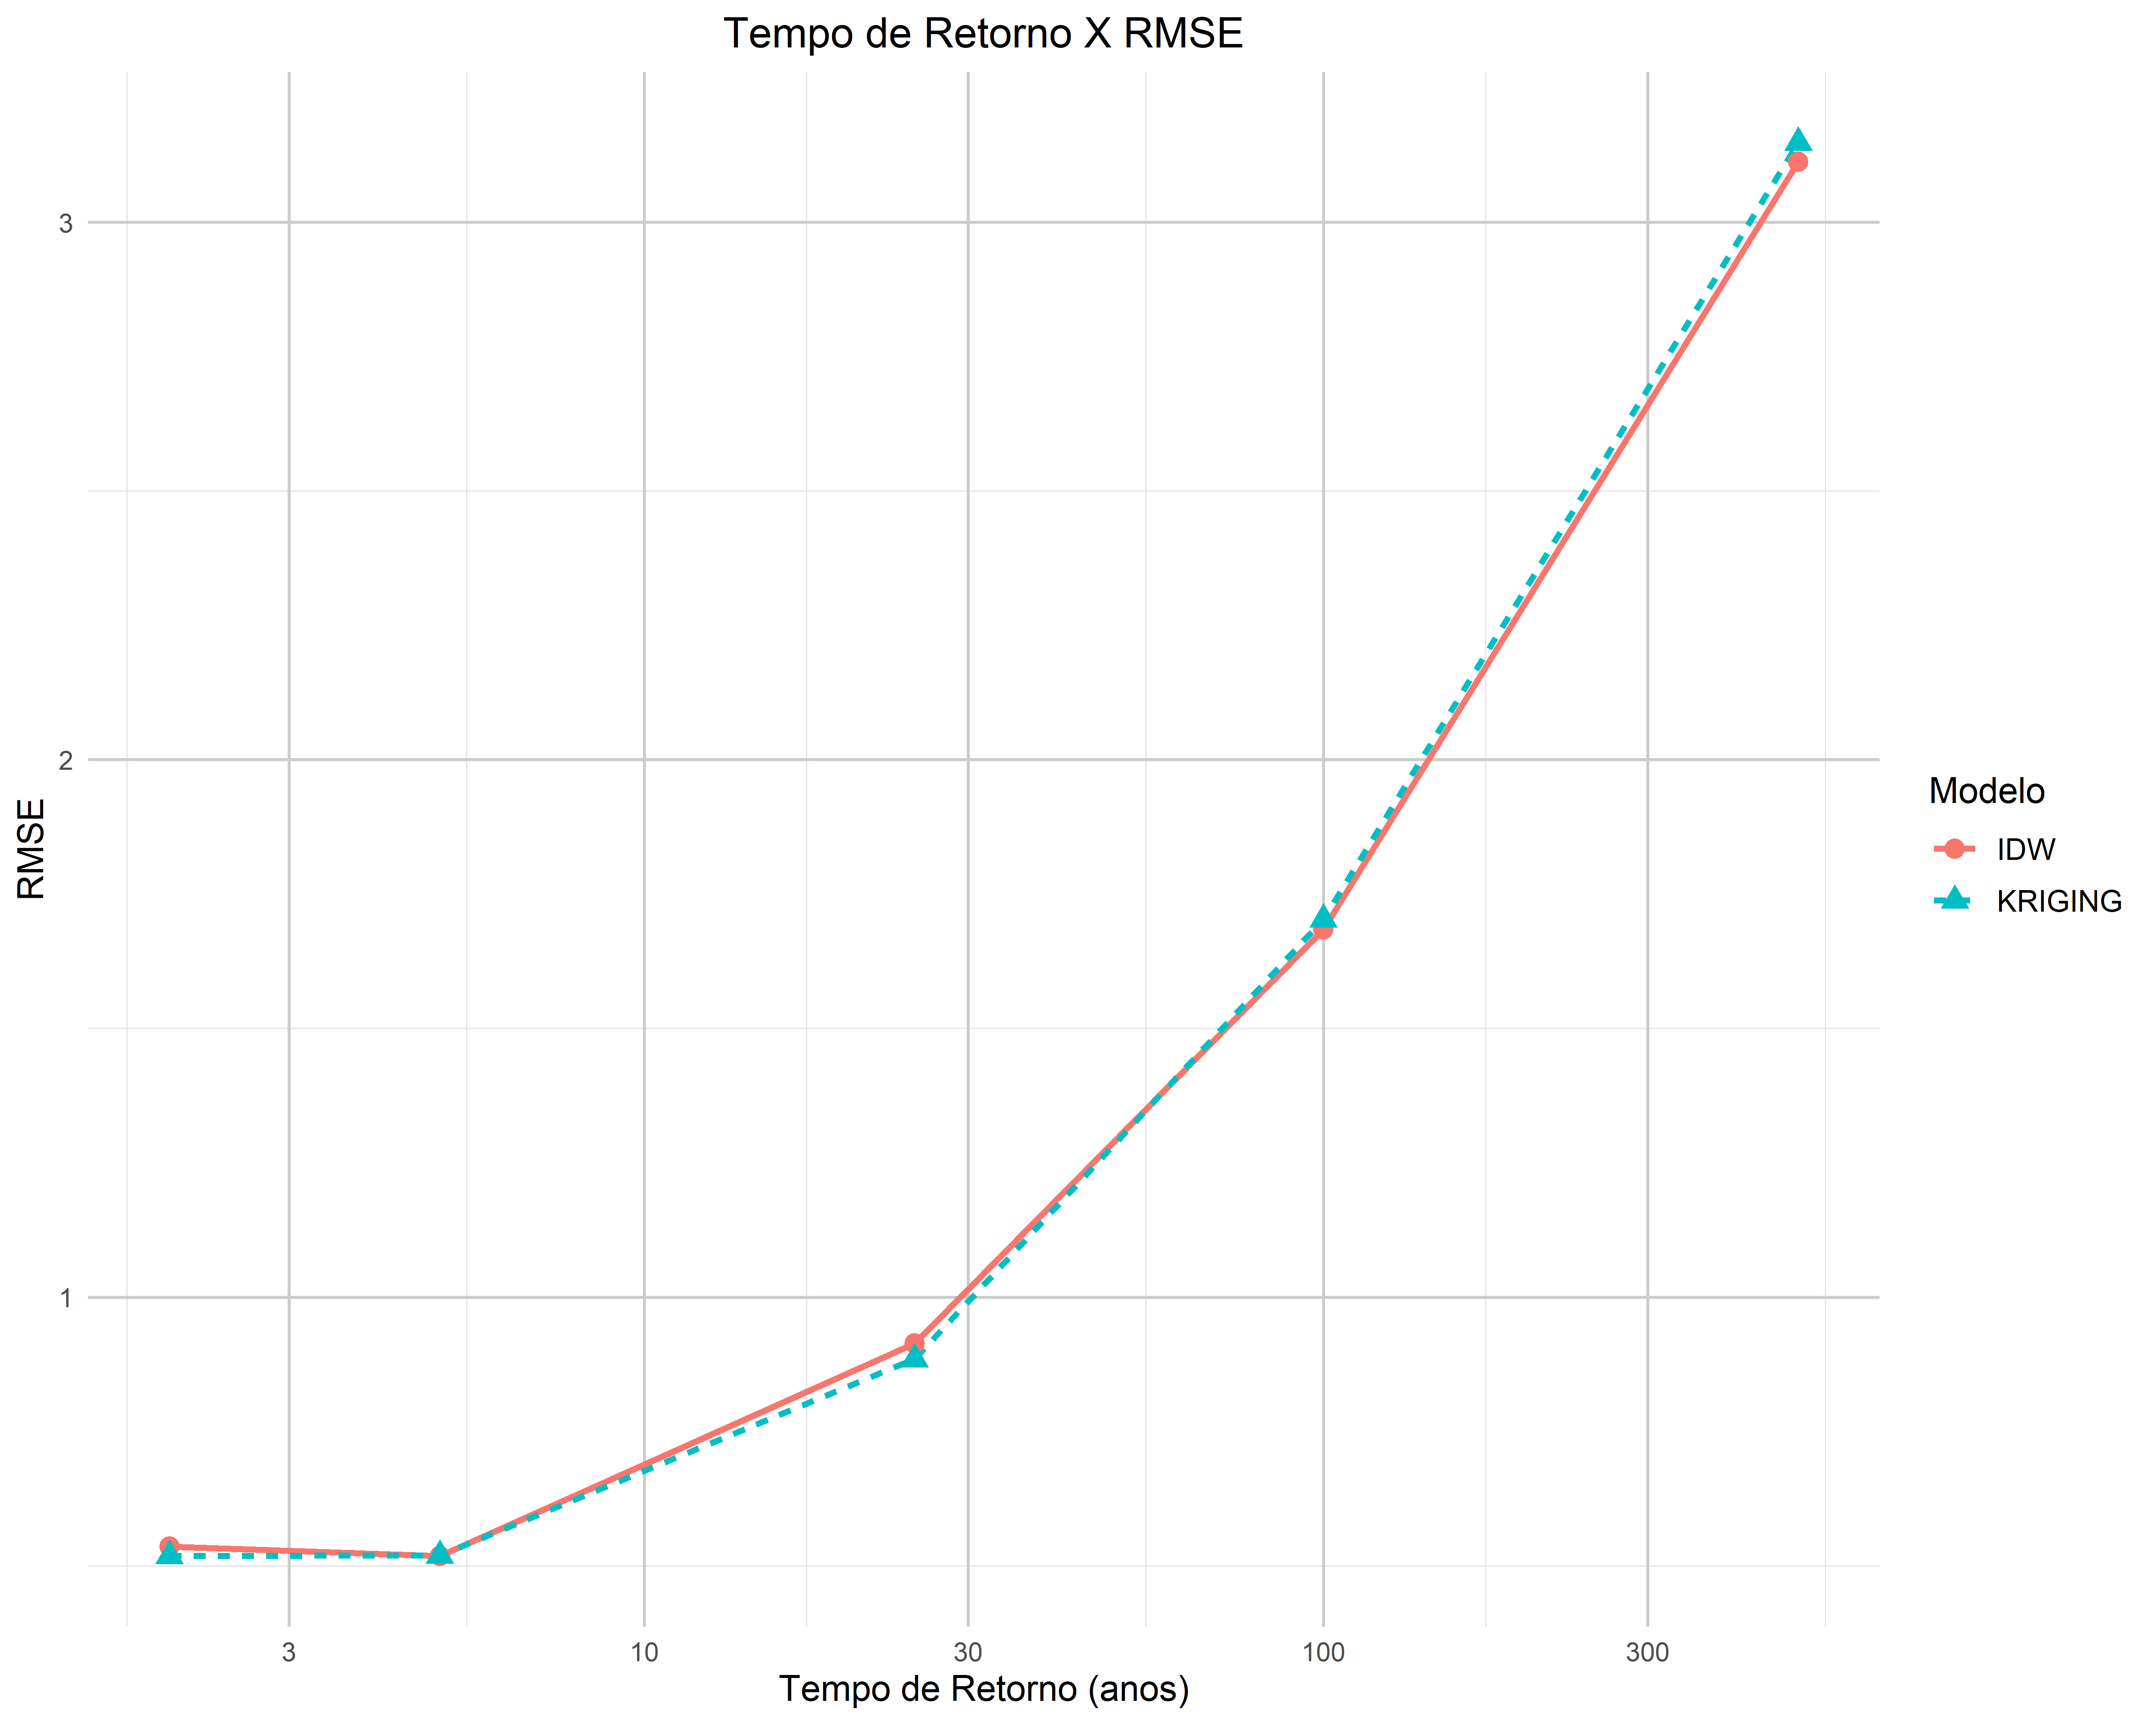
\includegraphics{Figuras/Figura15a.png}

}

\subcaption{\label{fig-Figura15a}RMSE em função do tempo de retorno para
cada modelo de interpolação}

\end{minipage}%
\newline
\begin{minipage}{\linewidth}

\centering{

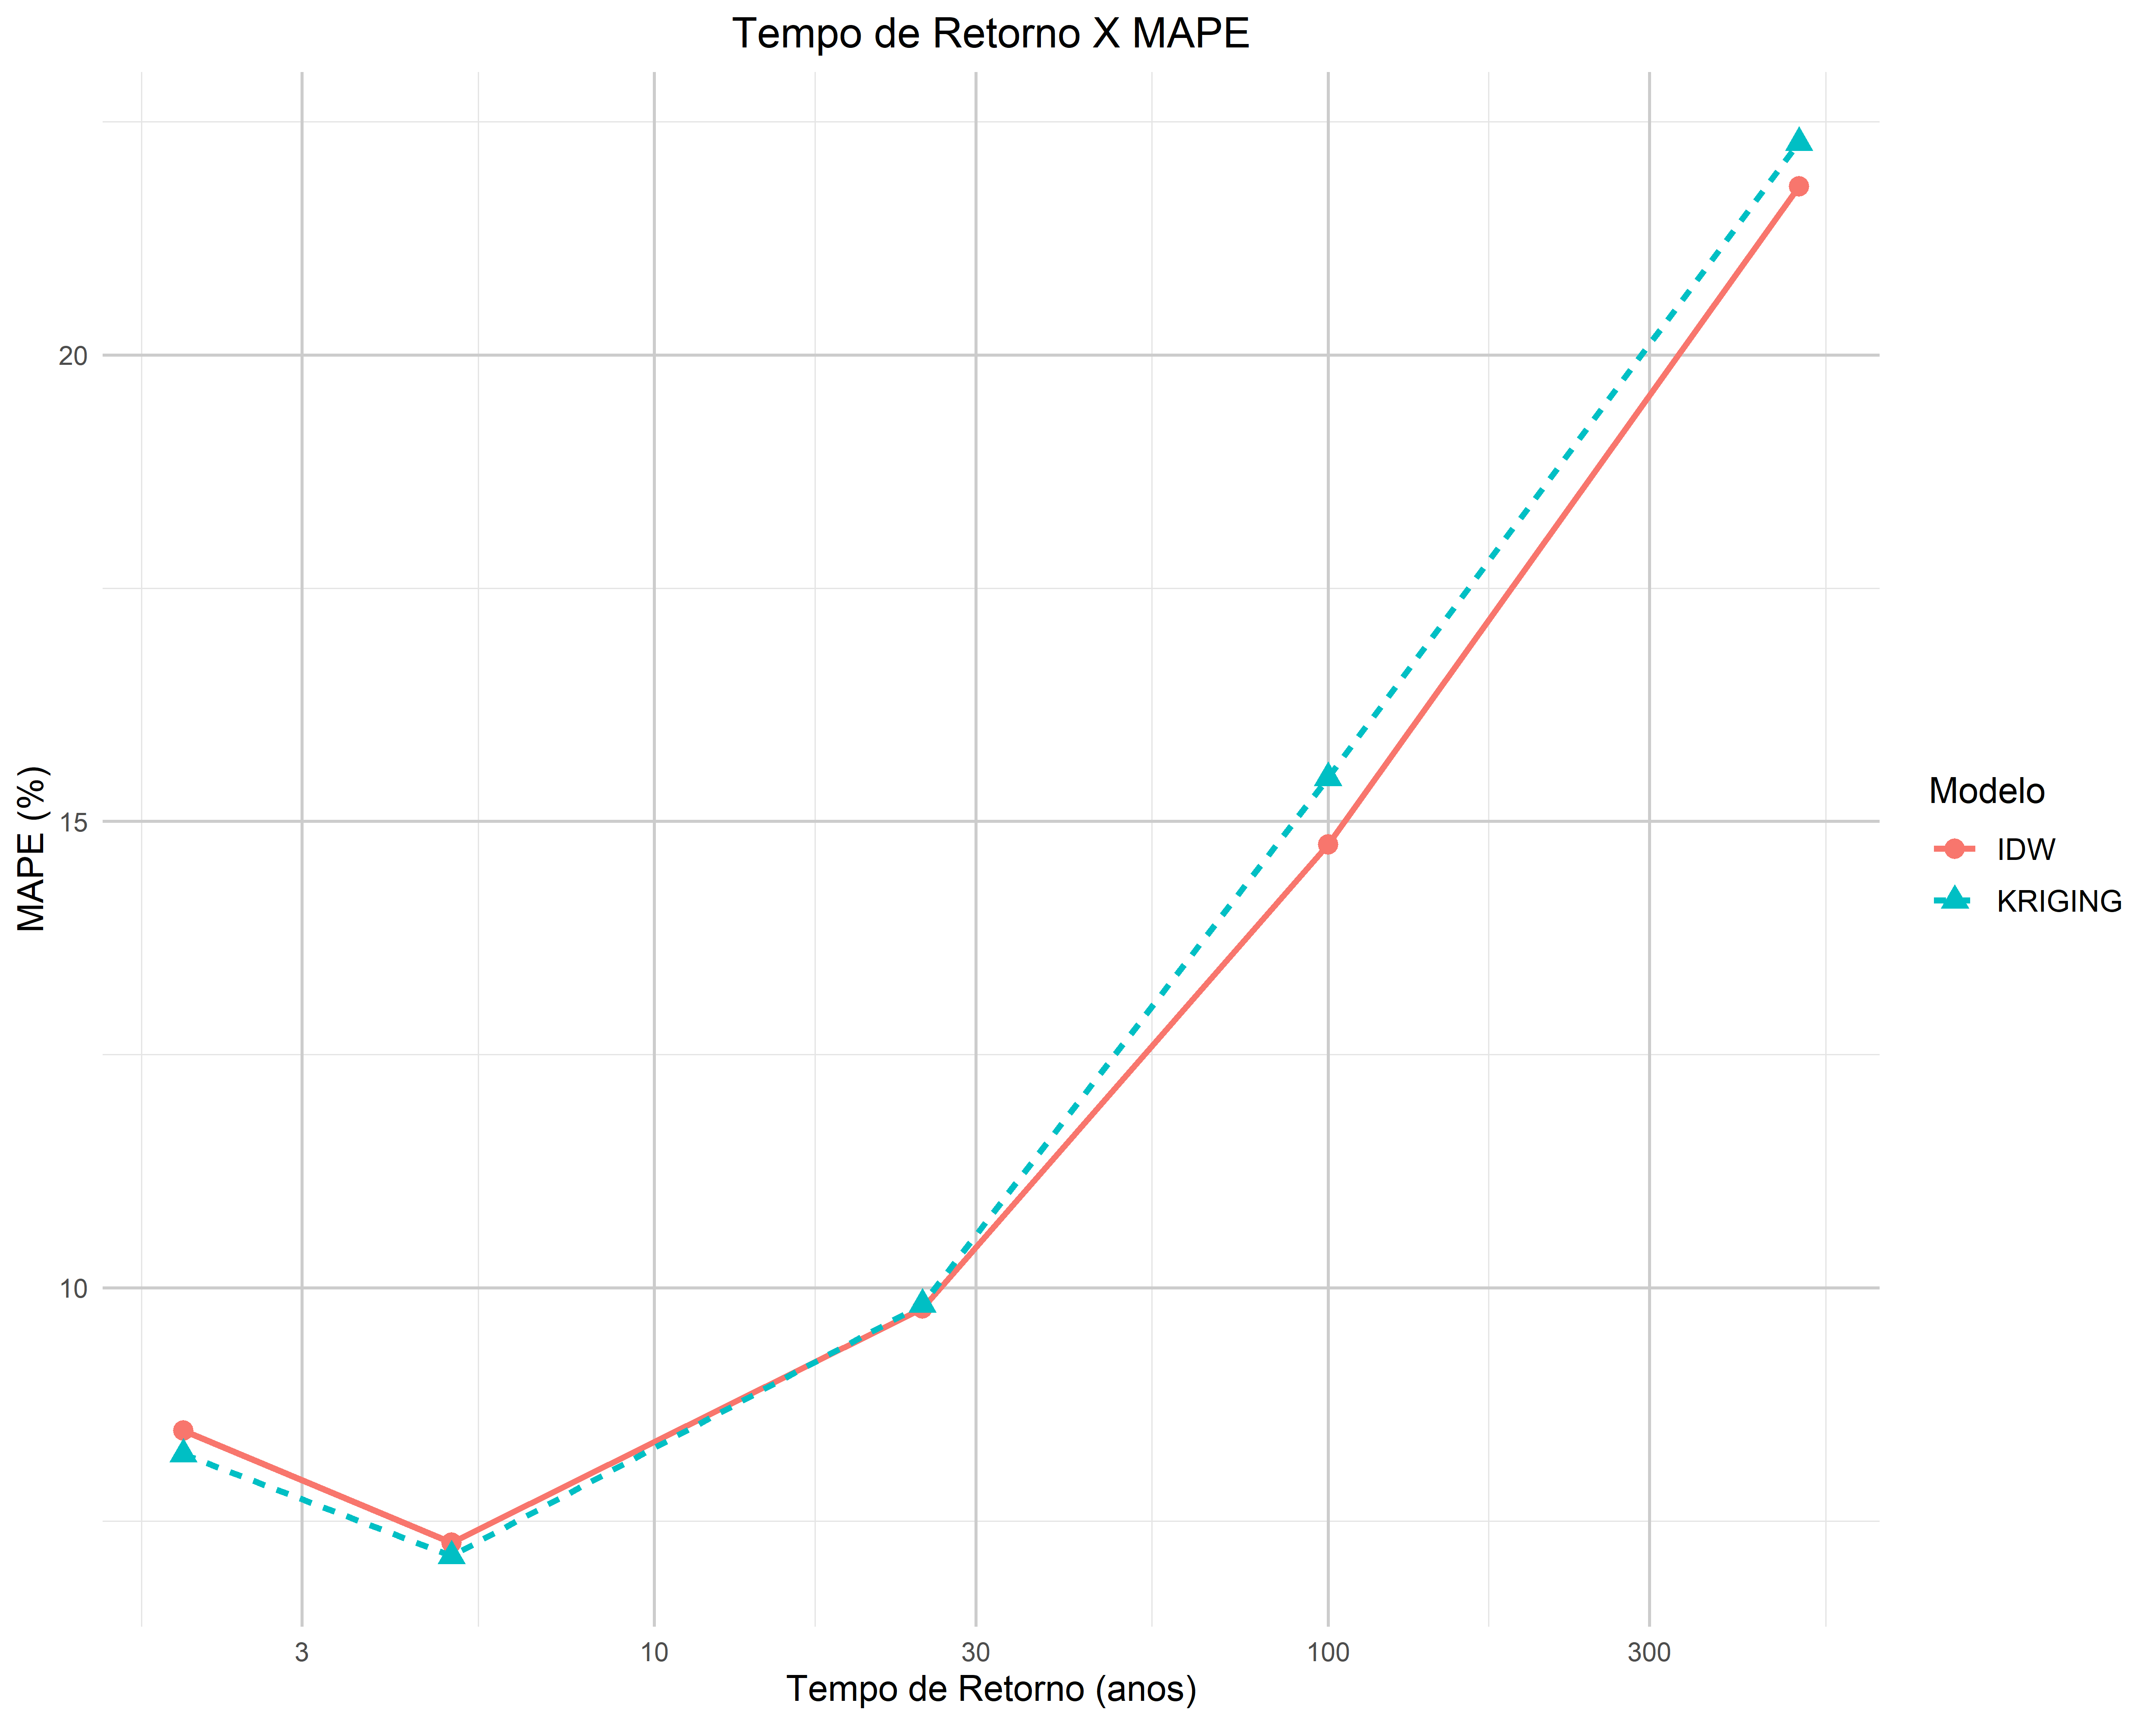
\includegraphics{Figuras/Figura15b.png}

}

\subcaption{\label{fig-Figura15b}MAPE em função do tempo de retorno para
cada modelo de interpolação}

\end{minipage}%

\caption{\label{fig-Figura15}Performance dos modelos de interpolação
considerando RMSE (a) e MAPE (b).}

\end{figure}%

\subsection{Incertezas entre os modelos de distribuições e métodos de
estimativa de
parâmetros}\label{incertezas-entre-os-modelos-de-distribuiuxe7uxf5es-e-muxe9todos-de-estimativa-de-paruxe2metros-1}

As Figuras 16 a 20 mostram os resultados obtidos para as diferenças
percentuais entre os valores máximos e mínimos obtidos a partir das três
distribuições testadas (GUM, GAM e GEV) e dos dois métodos de estimativa
de parâmetros empregados (MOM e MML). Portanto, apresenta-se em termos
percentuais, uma estimativa das incertezas em relação às distribuições e
métodos de estimativa de parâmetros empregados. Verifica-se, conforme
esperado, que quanto maior o tempo de retorno maior a variância entre os
valores calculados e, portanto, maior a incerteza. Para os tempos de
retorno entre 2 a 25 anos, as diferenças atingiram no máximo cerca de
40\%, enquanto para tempos de retorno entre 100 e 500 anos, essas
diferenças podem ultrapassar 50\% chegando até cerca de 100\%. Outro
aspecto que pode ser observado comparando as figuras 16 a 20 com as
figuras 10 a 15 é que as maiores incertezas, não necessariamente estão
associadas as estações que apresentam os maiores volumes de chuvas.
Dessa forma, cada estação possui suas características intrínsecas
relacionadas à incertezas.

\begin{figure}

\centering{

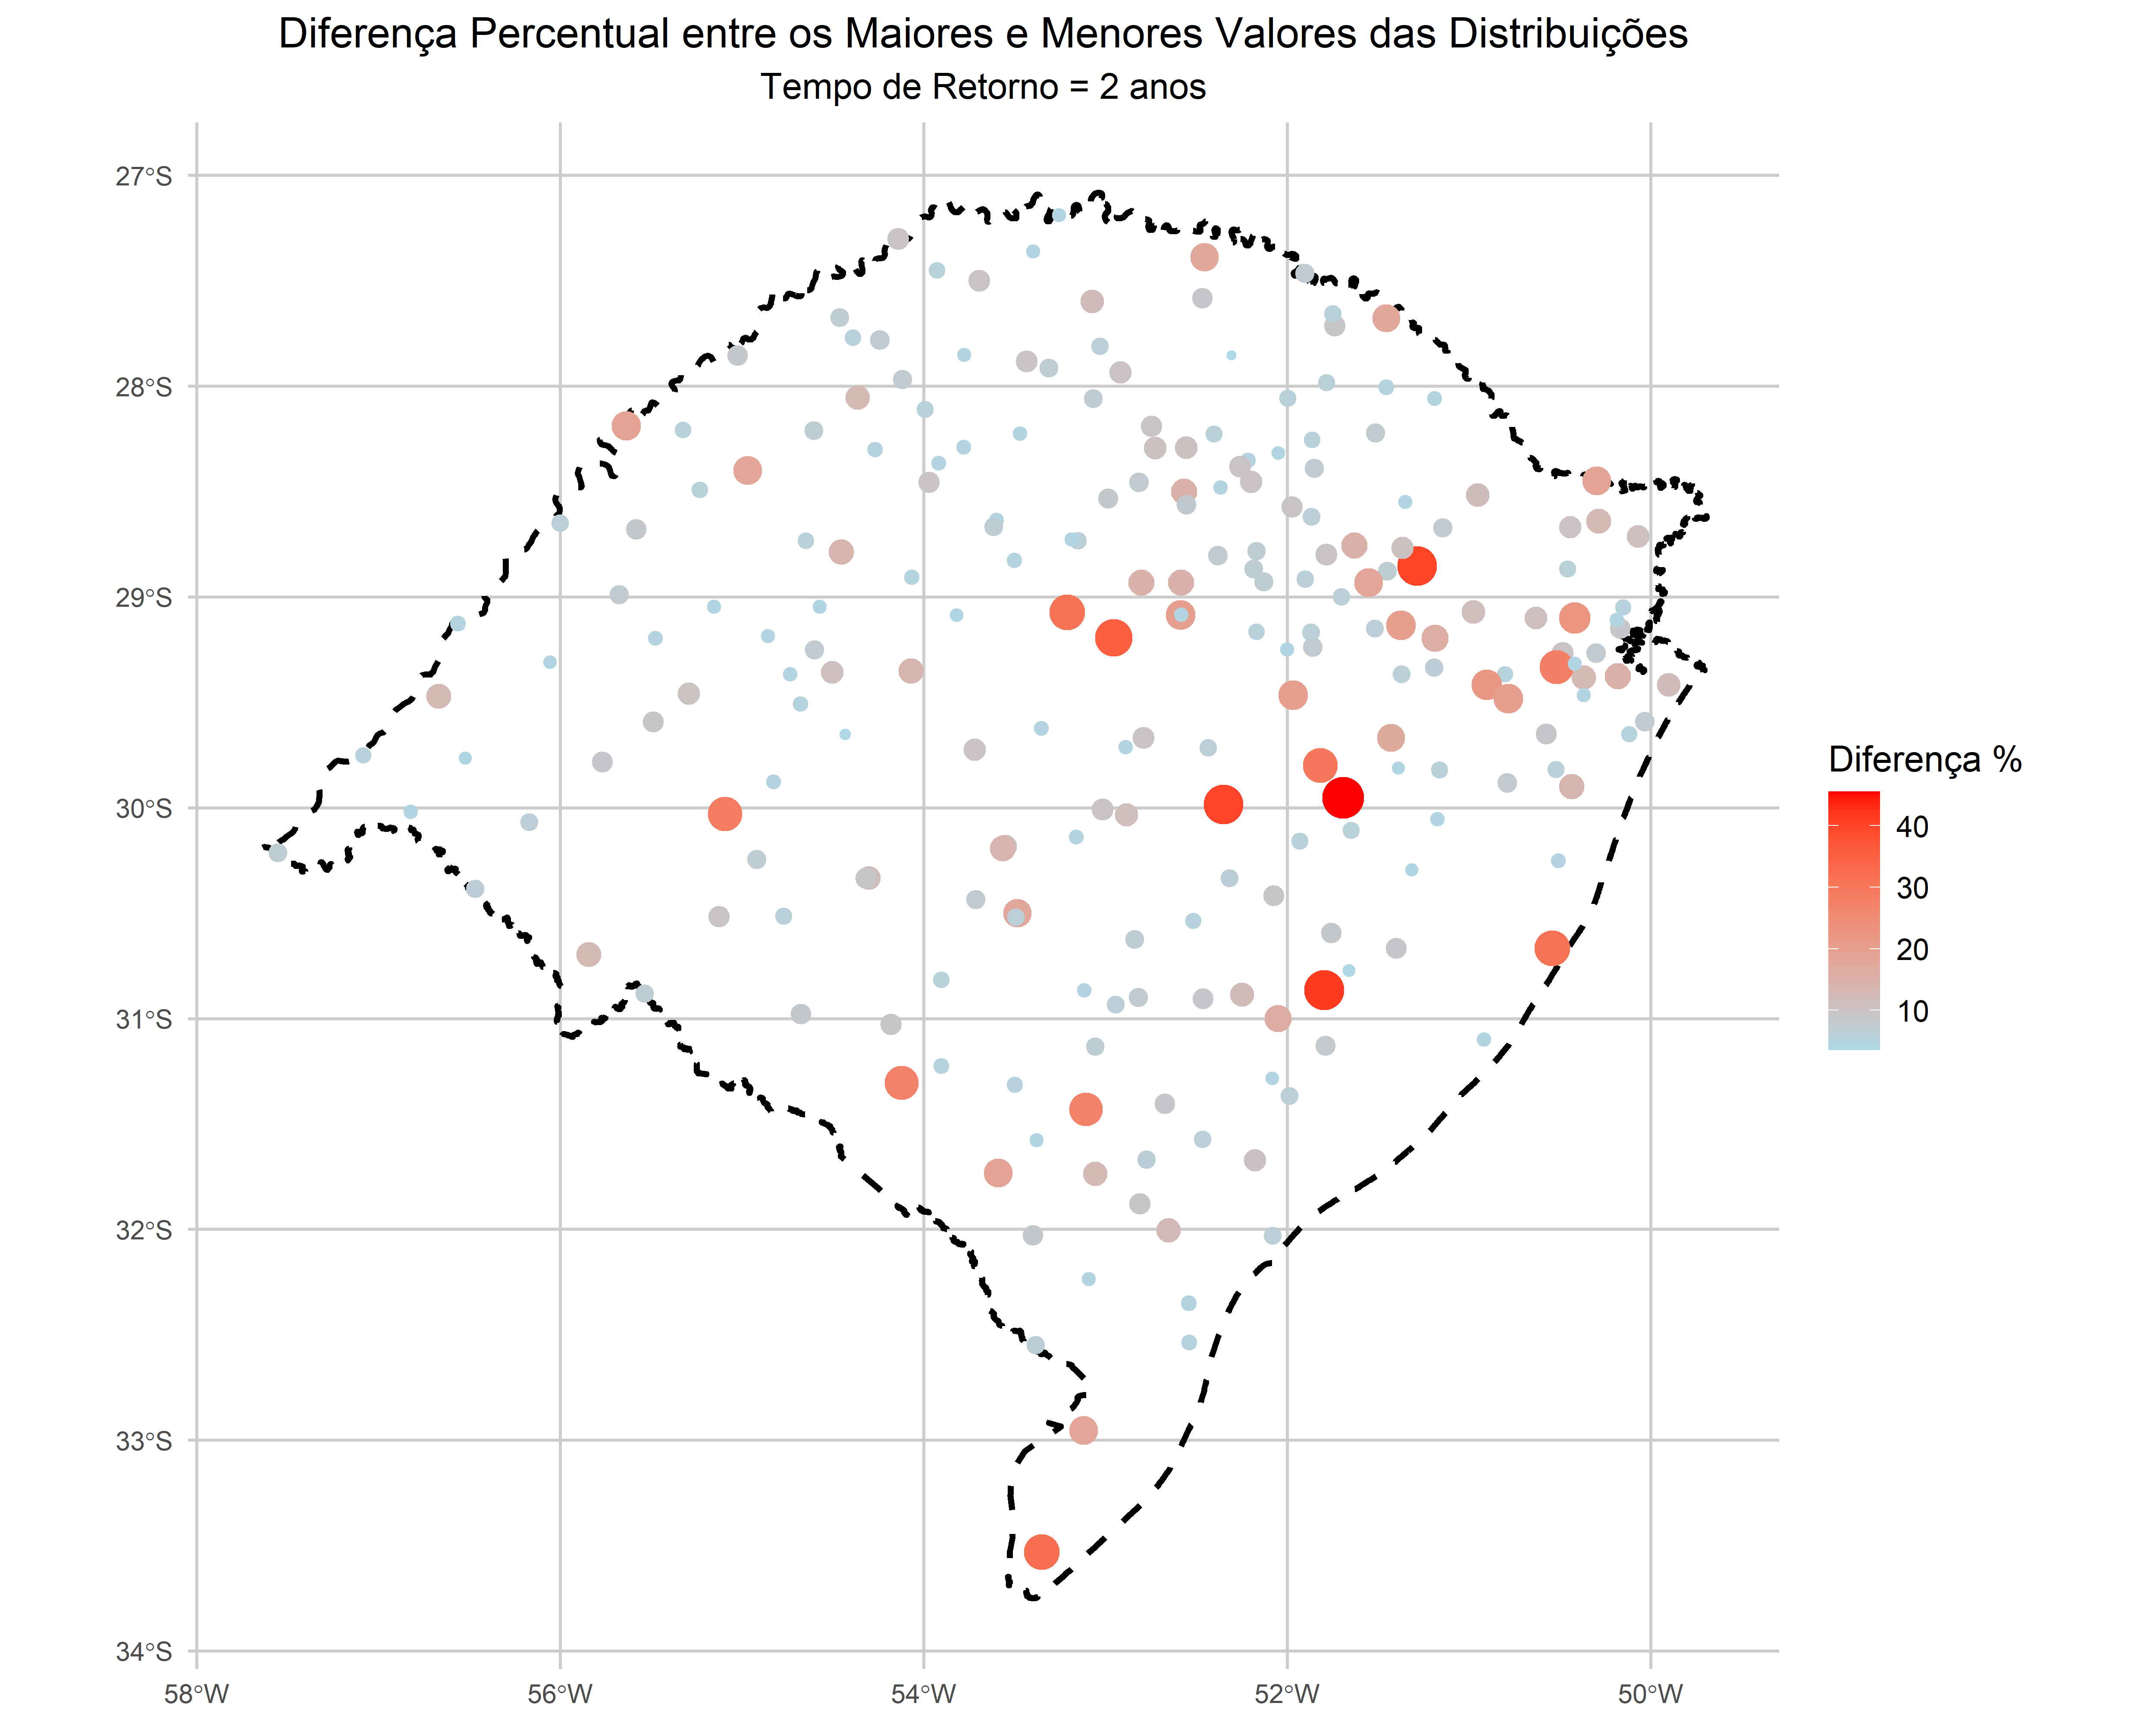
\includegraphics{Figuras/Figura16.png}

}

\caption{\label{fig-Figura16}Diferença percentual entre os maiores e
menores valores obtidos para a chuva de duração de 24 horas calculada a
partir das distribuições GUM, GAM e GEV e os métodos MOM e MML para o
tempo de retorno de 2 anos}

\end{figure}%

\begin{figure}

\centering{

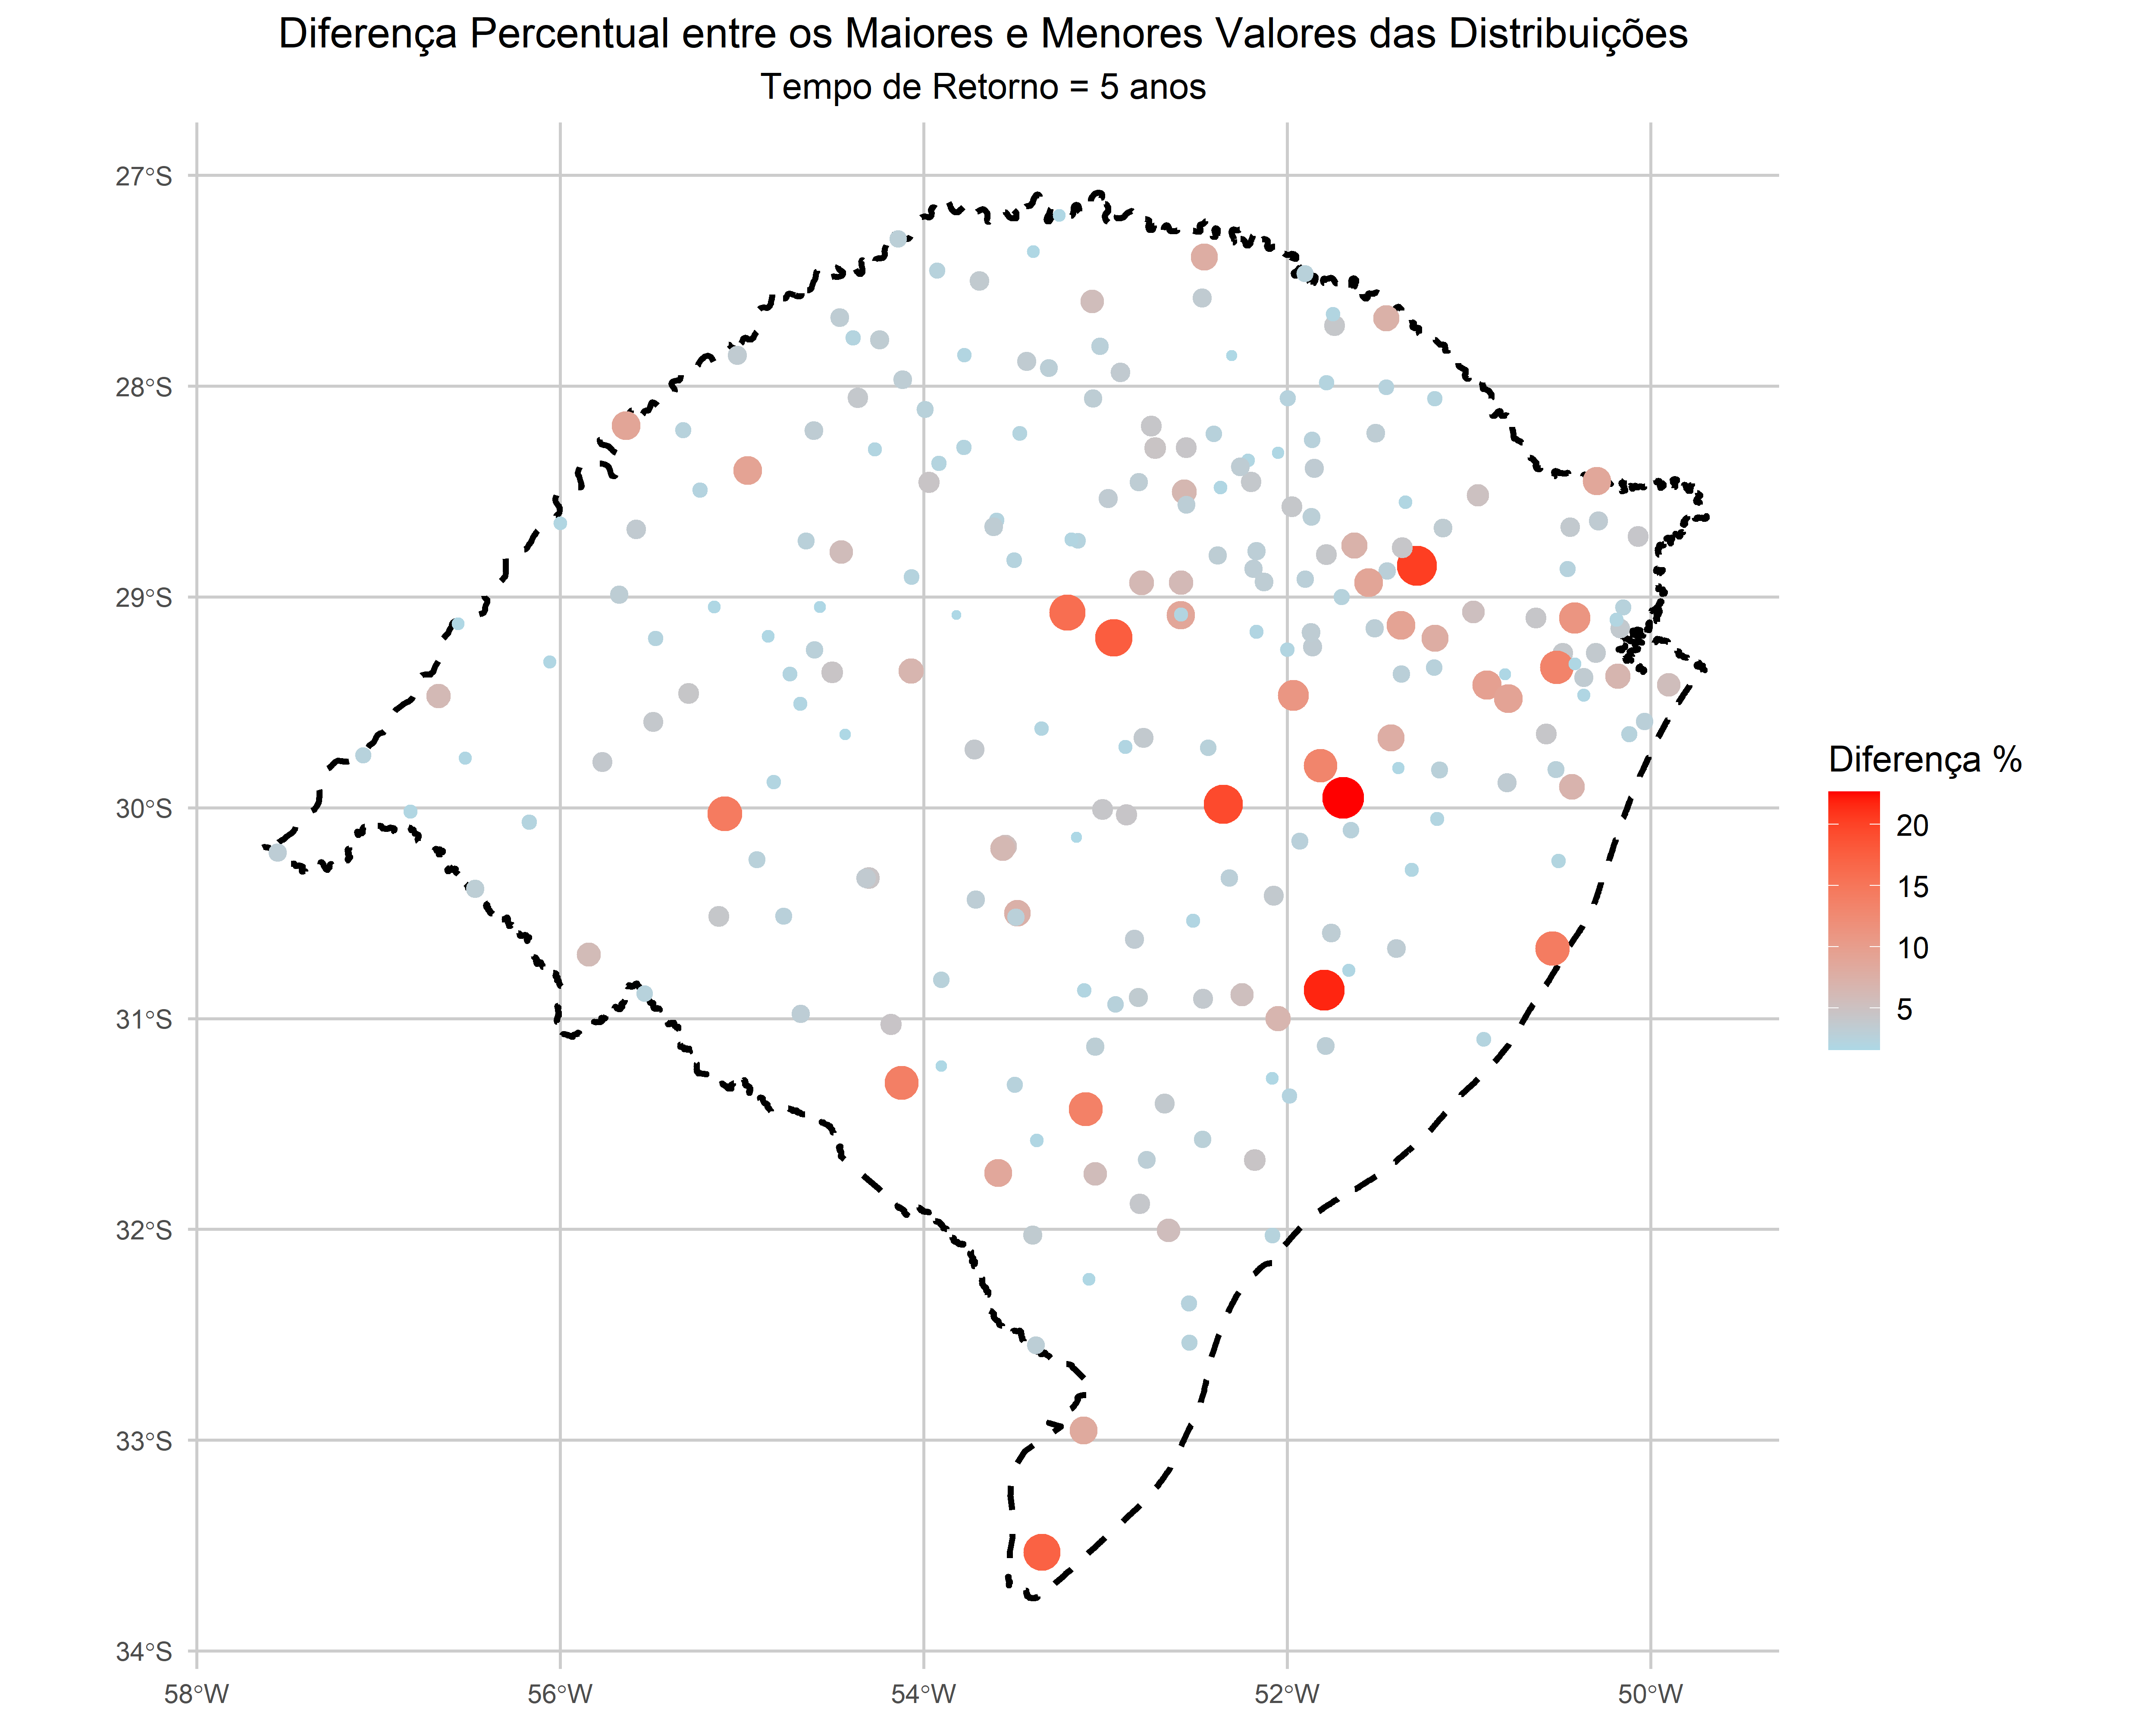
\includegraphics{Figuras/Figura17.png}

}

\caption{\label{fig-Figura17}Diferença percentual entre os maiores e
menores valores obtidos para a chuva de duração de 24 horas calculada a
partir das distribuições GUM, GAM e GEV e os métodos MOM e MML para o
tempo de retorno de 5 anos}

\end{figure}%

\begin{figure}

\centering{

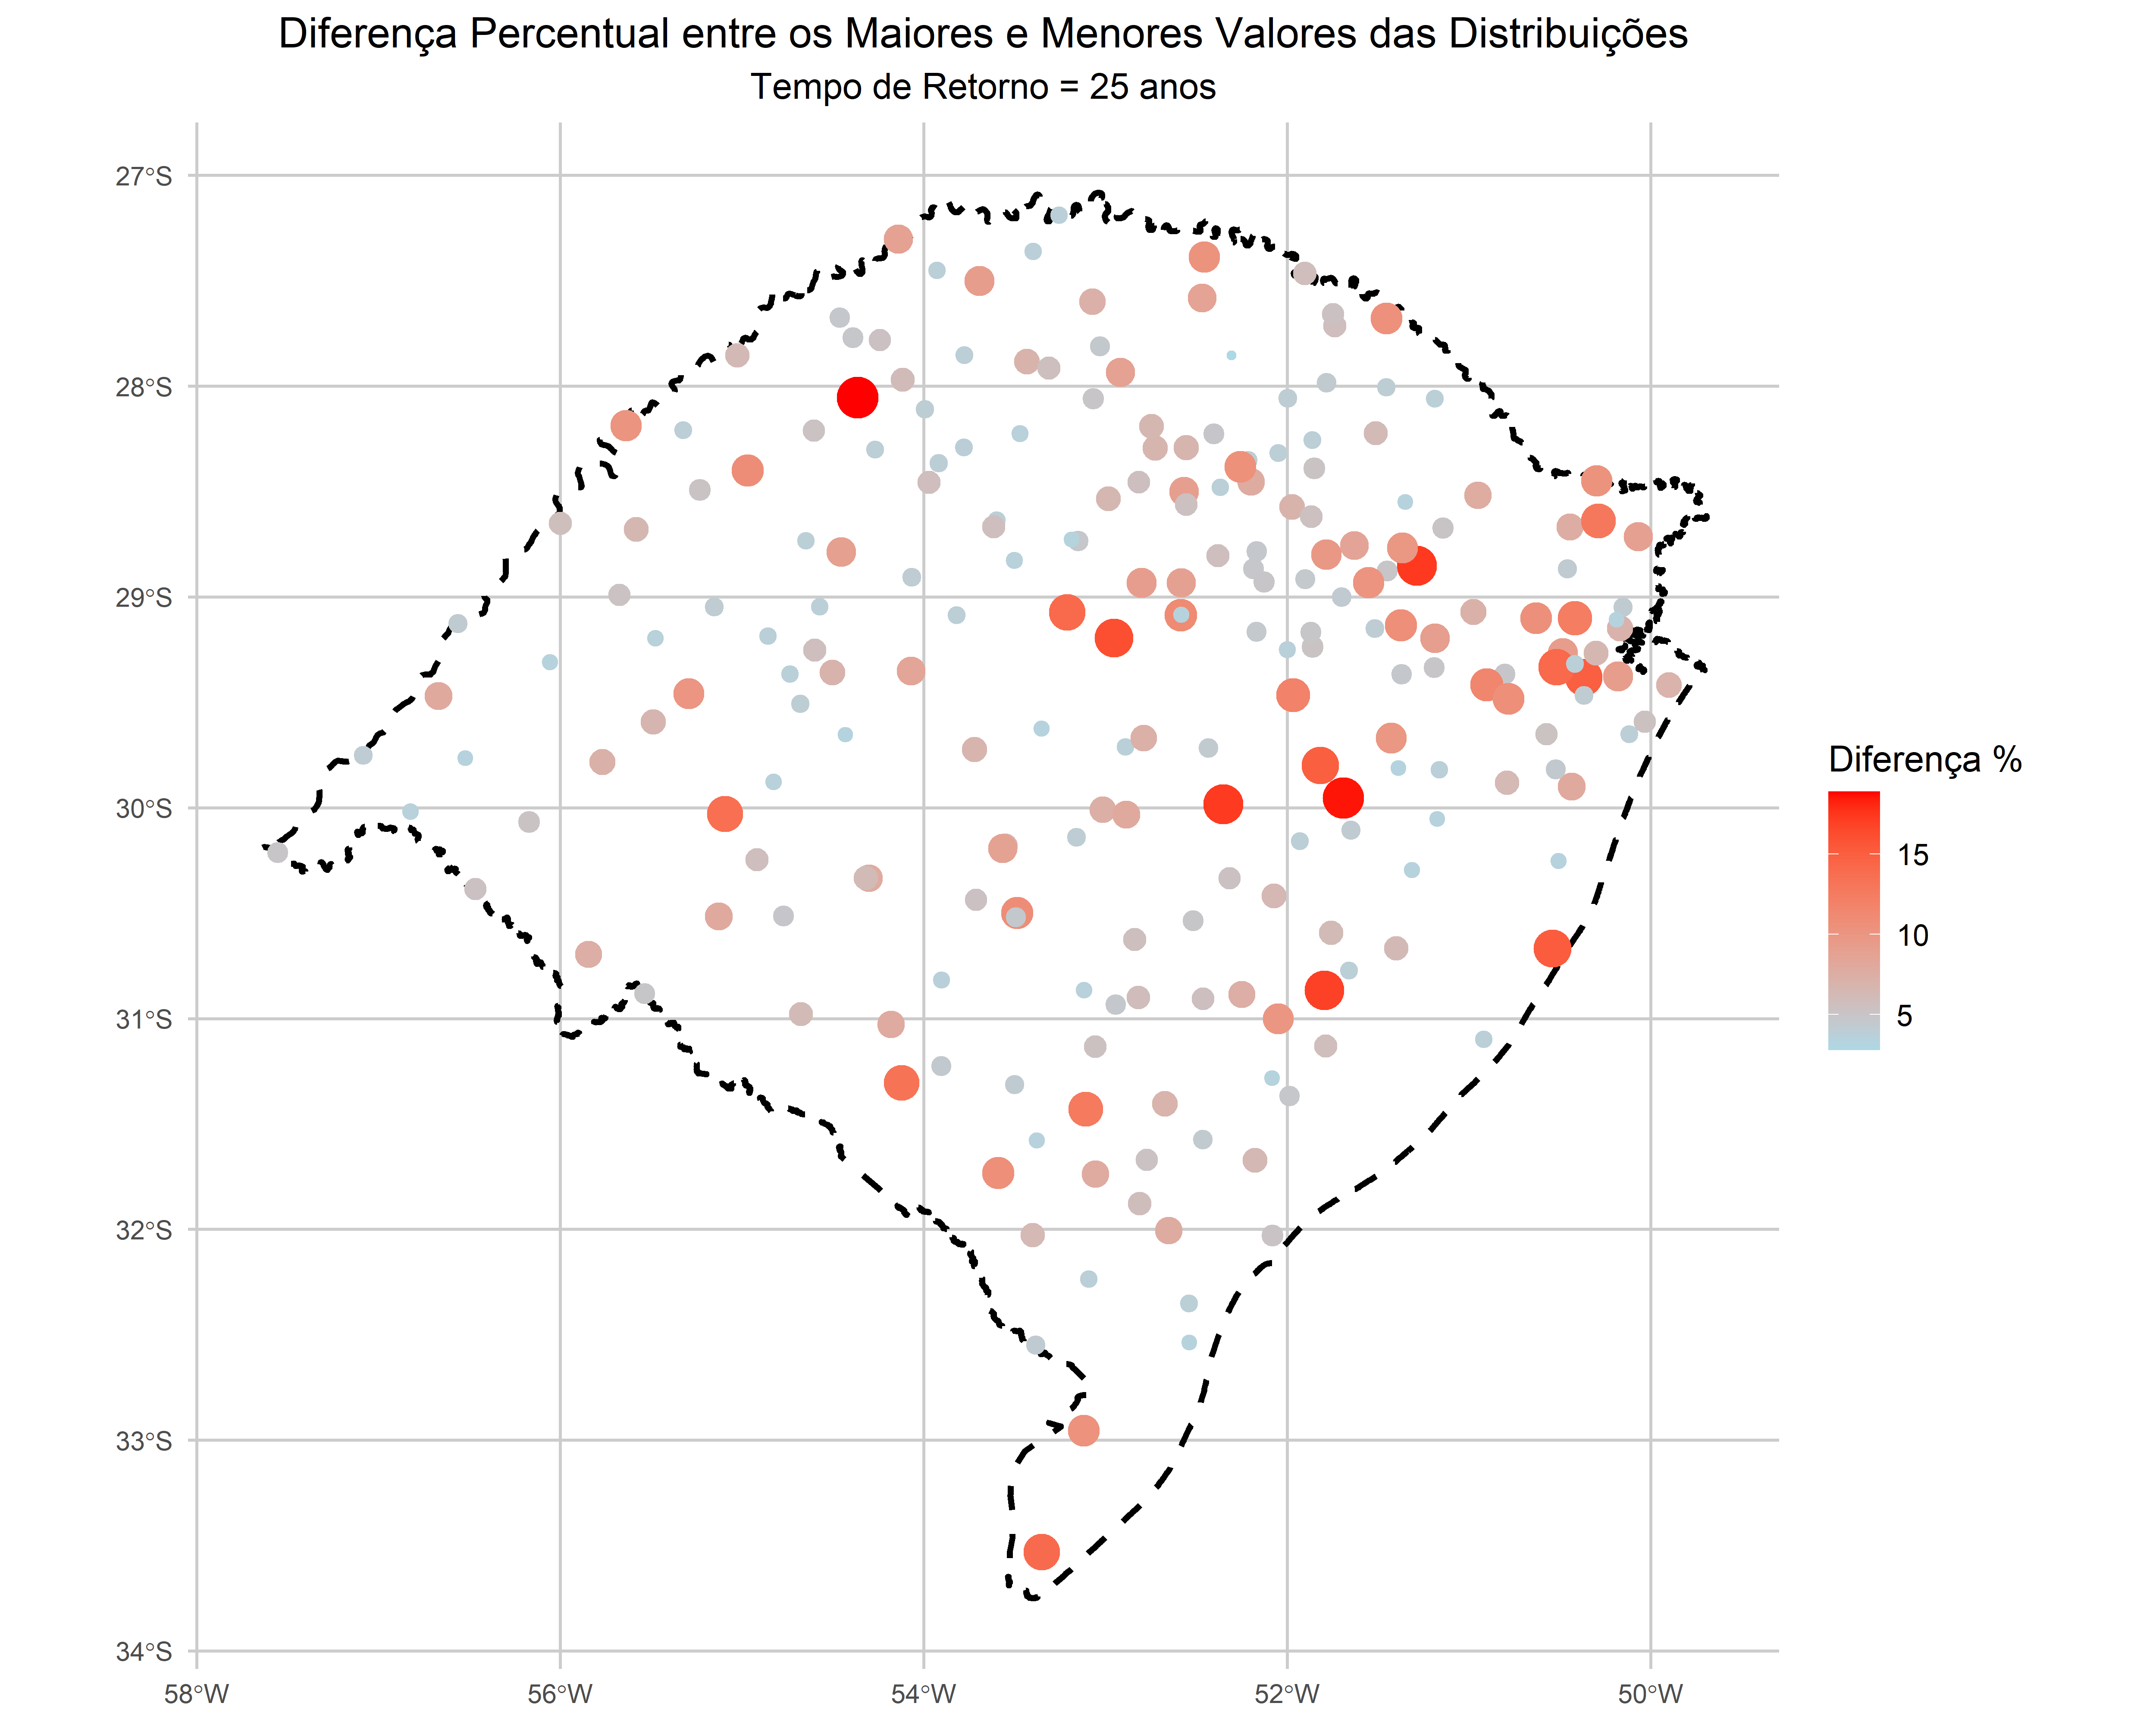
\includegraphics{Figuras/Figura18.png}

}

\caption{\label{fig-Figura18}Diferença percentual entre os maiores e
menores valores obtidos para a chuva de duração de 24 horas calculada a
partir das distribuições GUM, GAM e GEV e os métodos MOM e MML para o
tempo de retorno de 25 anos}

\end{figure}%

\begin{figure}

\centering{

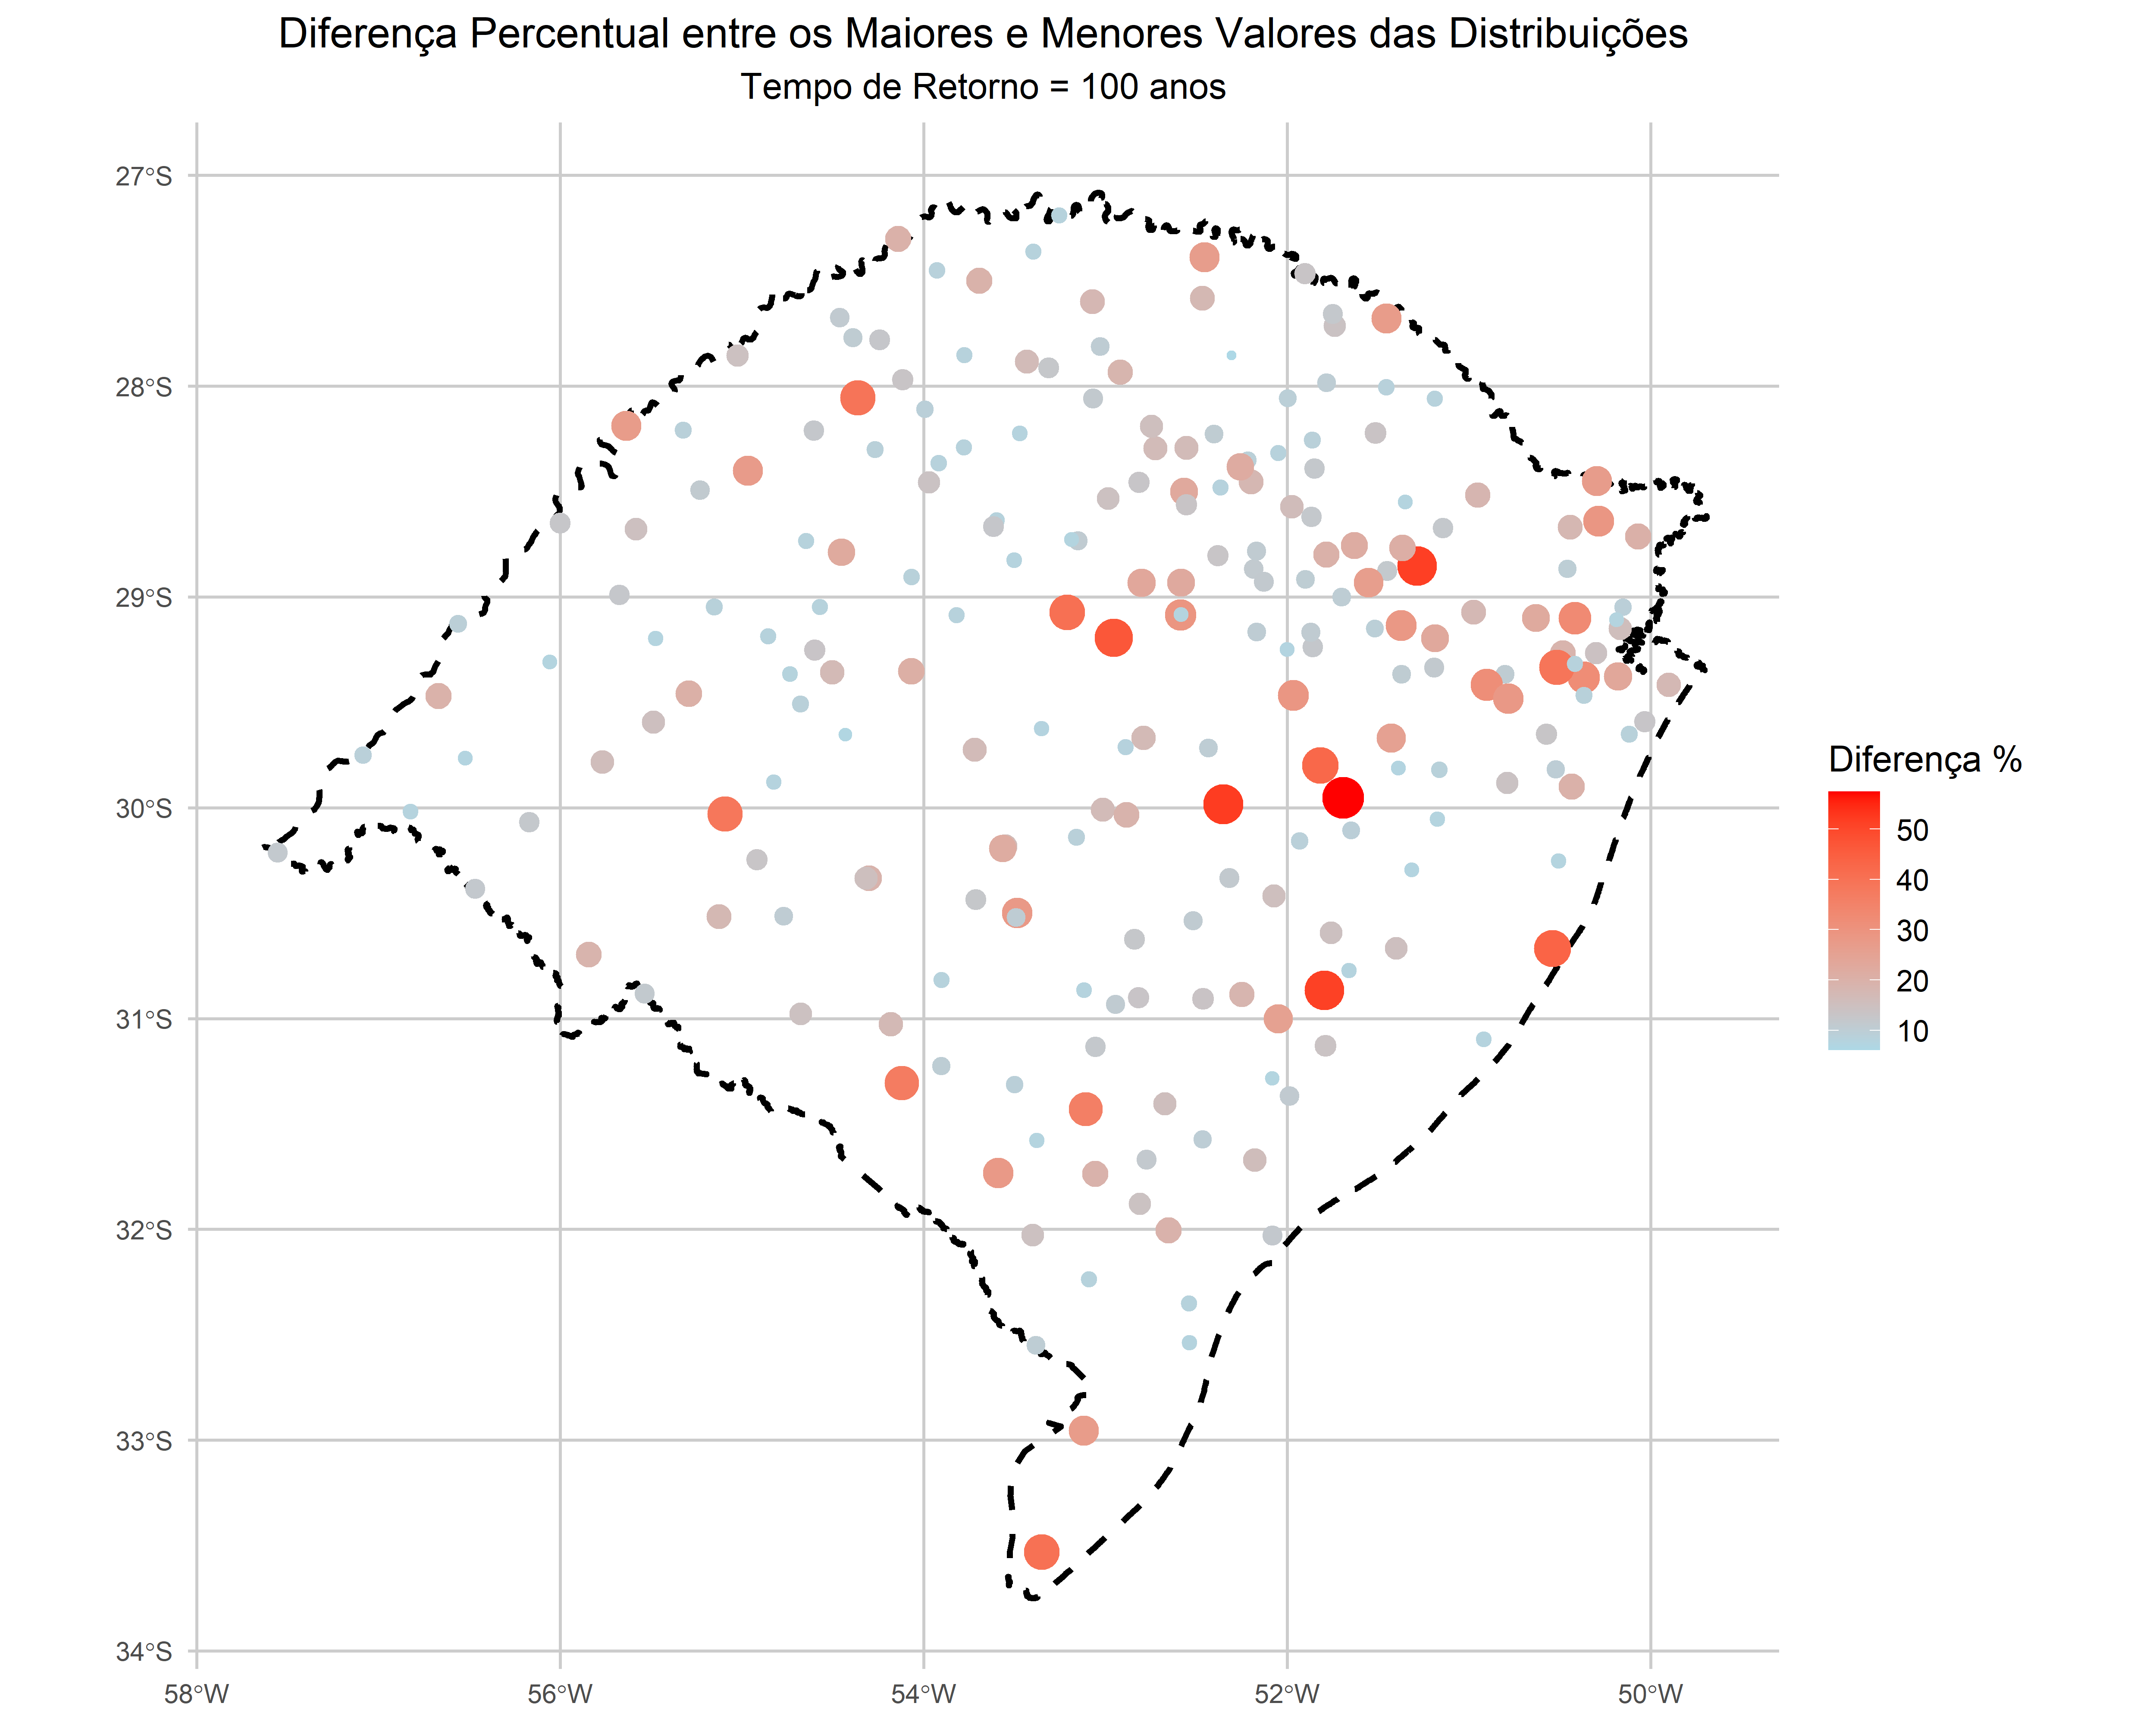
\includegraphics{Figuras/Figura19.png}

}

\caption{\label{fig-Figura19}Diferença percentual entre os maiores e
menores valores obtidos para a chuva de duração de 24 horas calculada a
partir das distribuições GUM, GAM e GEV e os métodos MOM e MML para o
tempo de retorno de 100 anos}

\end{figure}%

\begin{figure}

\centering{

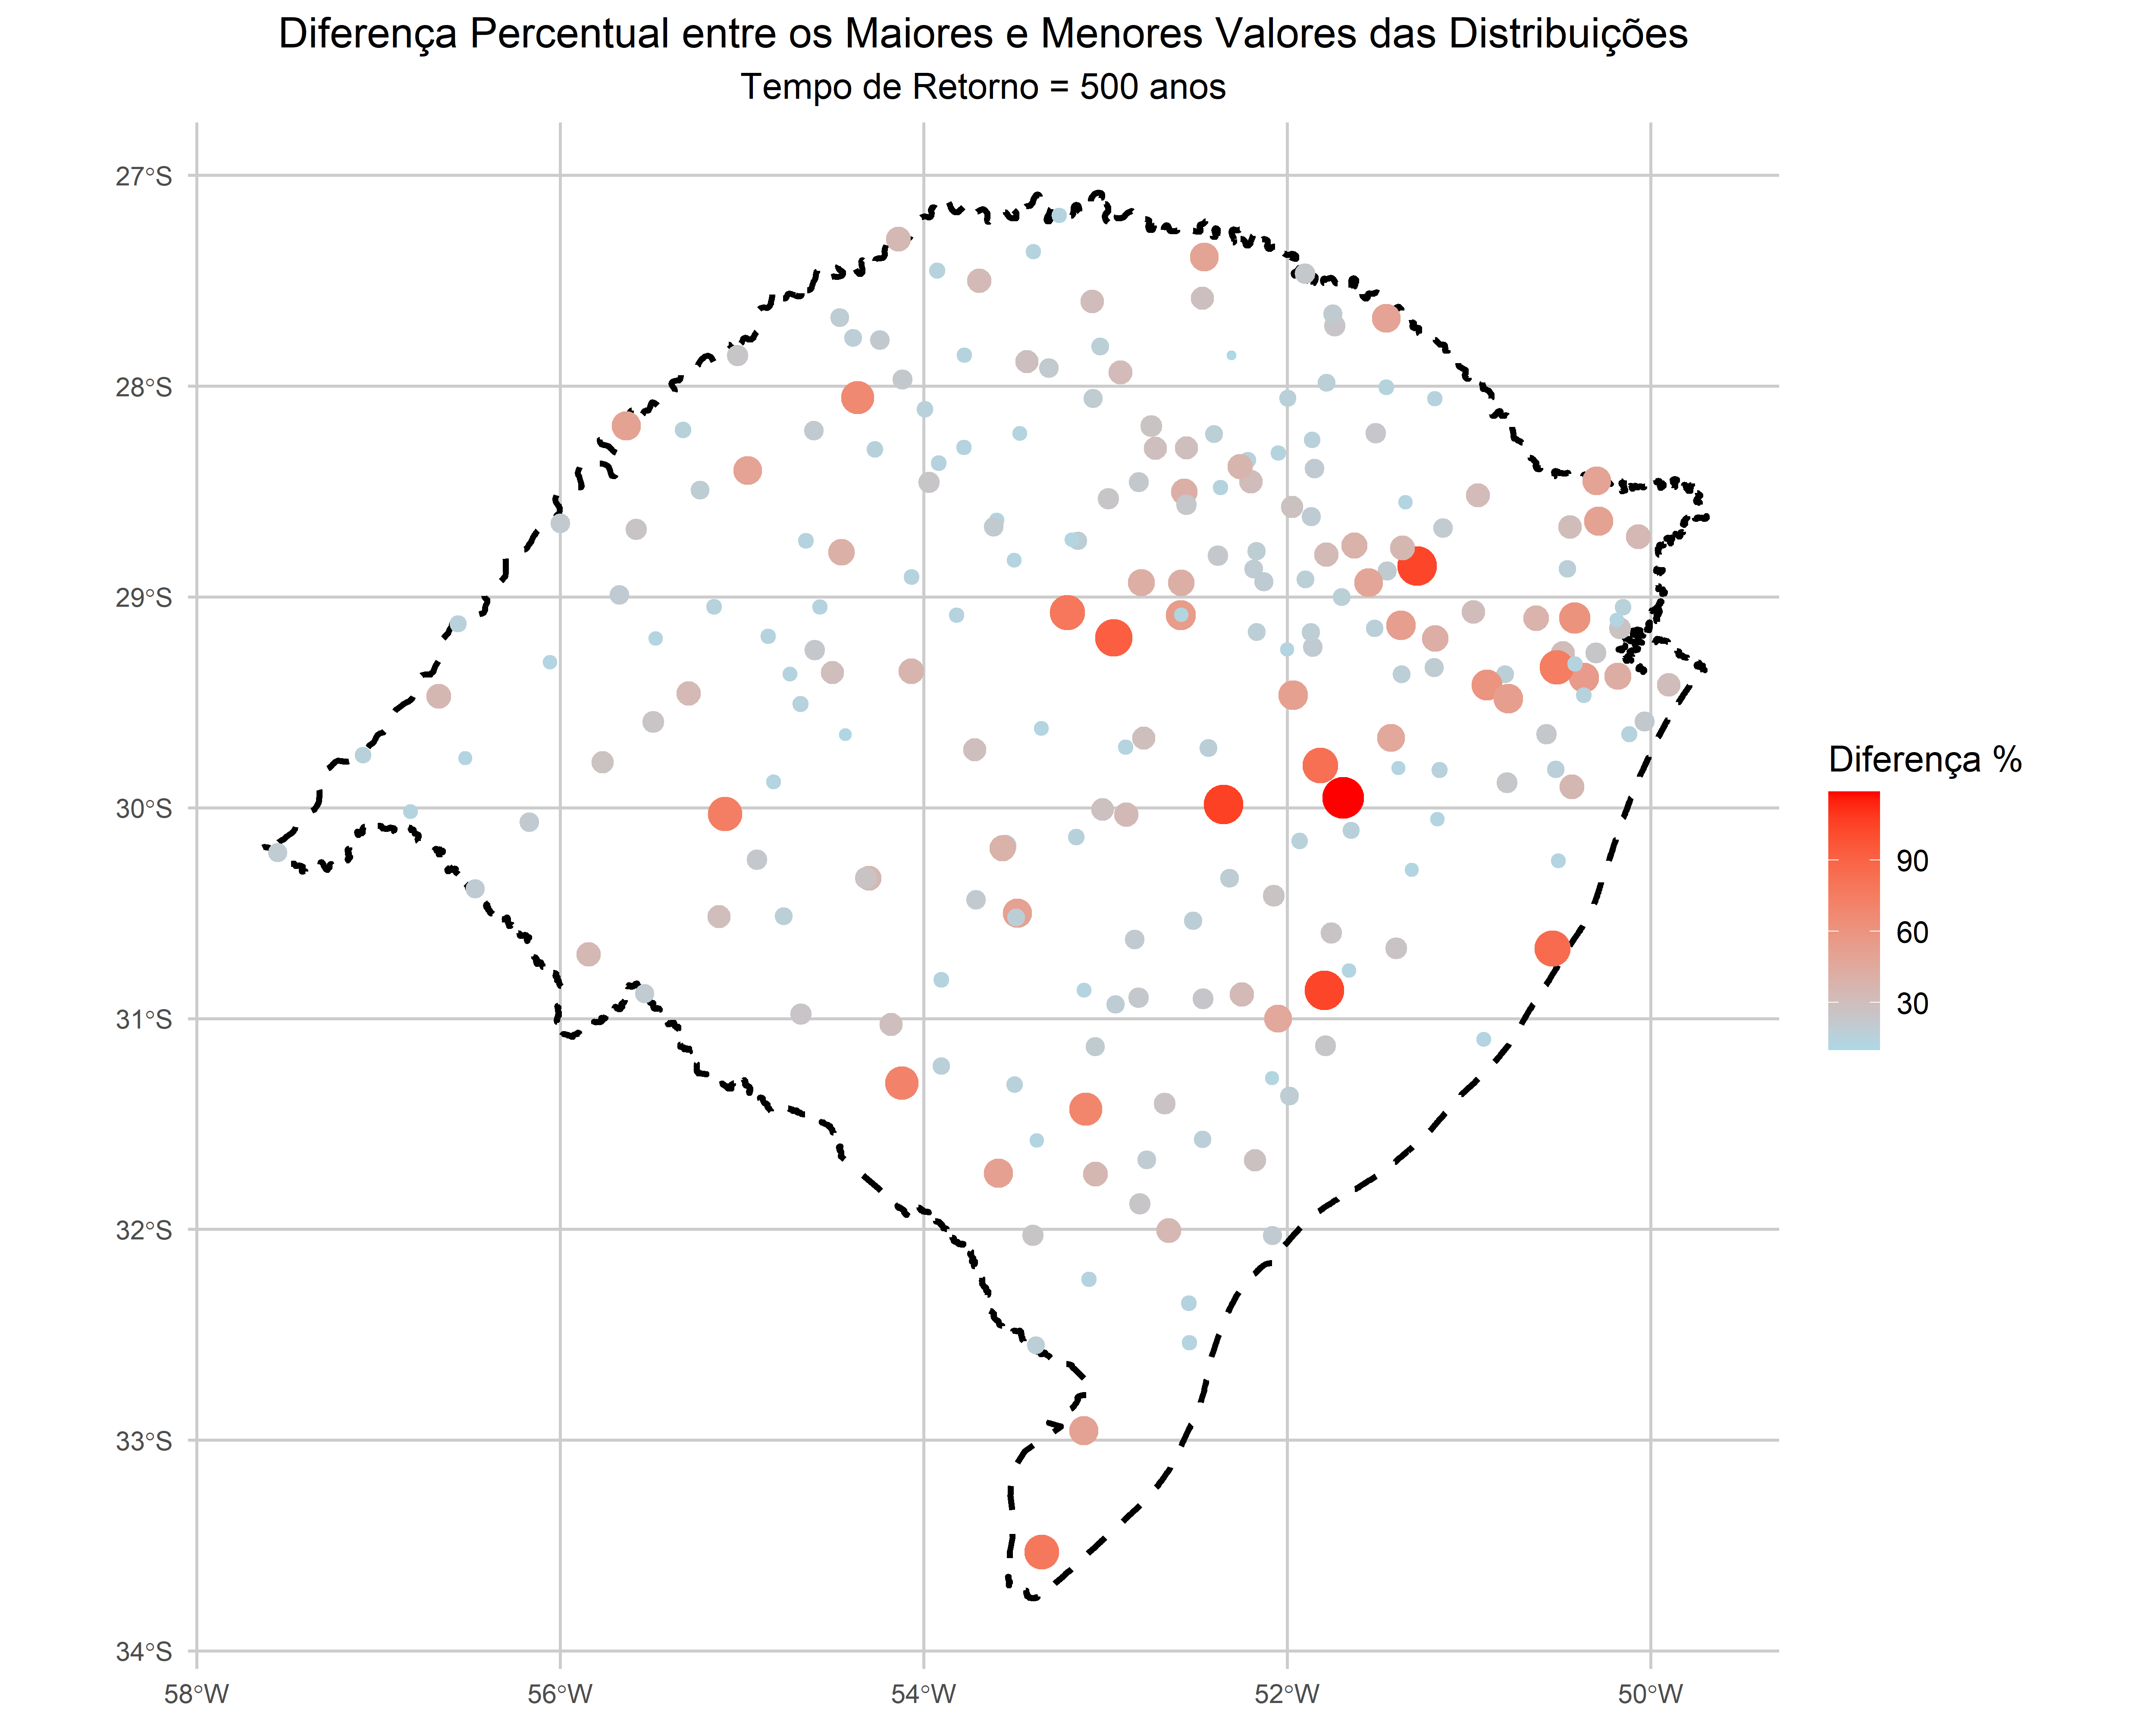
\includegraphics{Figuras/Figura20.png}

}

\caption{\label{fig-Figura20}Diferença percentual entre os maiores e
menores valores obtidos para a chuva de duração de 24 horas calculada a
partir das distribuições GUM, GAM e GEV e os métodos MOM e MML para o
tempo de retorno de 500 anos}

\end{figure}%

\subsection{Estimativa do erro entre as bases de dados em grade e as
estações
pluviométricas}\label{estimativa-do-erro-entre-as-bases-de-dados-em-grade-e-as-estauxe7uxf5es-pluviomuxe9tricas-1}

As Figuras 21 a 25 apresentam os resultados comparativos das diferenças
percentuais entre as intensidades de chuva de duração de 24 horas
previstas a partir das IDFs ajustadas para as estações e para as bases
XAVIER (a) e CHIRPS (b) considerando os tempos de retorno de 2, 5, 25,
100 e 500 anos, respectivamente. Os valores negativos nos percentuais
indicam uma tendência de se subestimar os valores calculados a partir
das estações quando se utilizam as IDFs obtidas a partir dos dados em
grade. As cores mais avermelhadas mostram diferenças percentuais
negativas mais acentuadas. Percebe-se que para ambas as bases há uma
tendência espacial de subestimar os valores de chuva em relação àqueles
obtidos a partir das estações. Essas diferenças tendem a aumentar em
função do tempo de retorno considerado ultrapassando uma diferença de
100\% para tempos de retorno maiores (100 e 500 anos).

\begin{figure}

\begin{minipage}{\linewidth}

\centering{

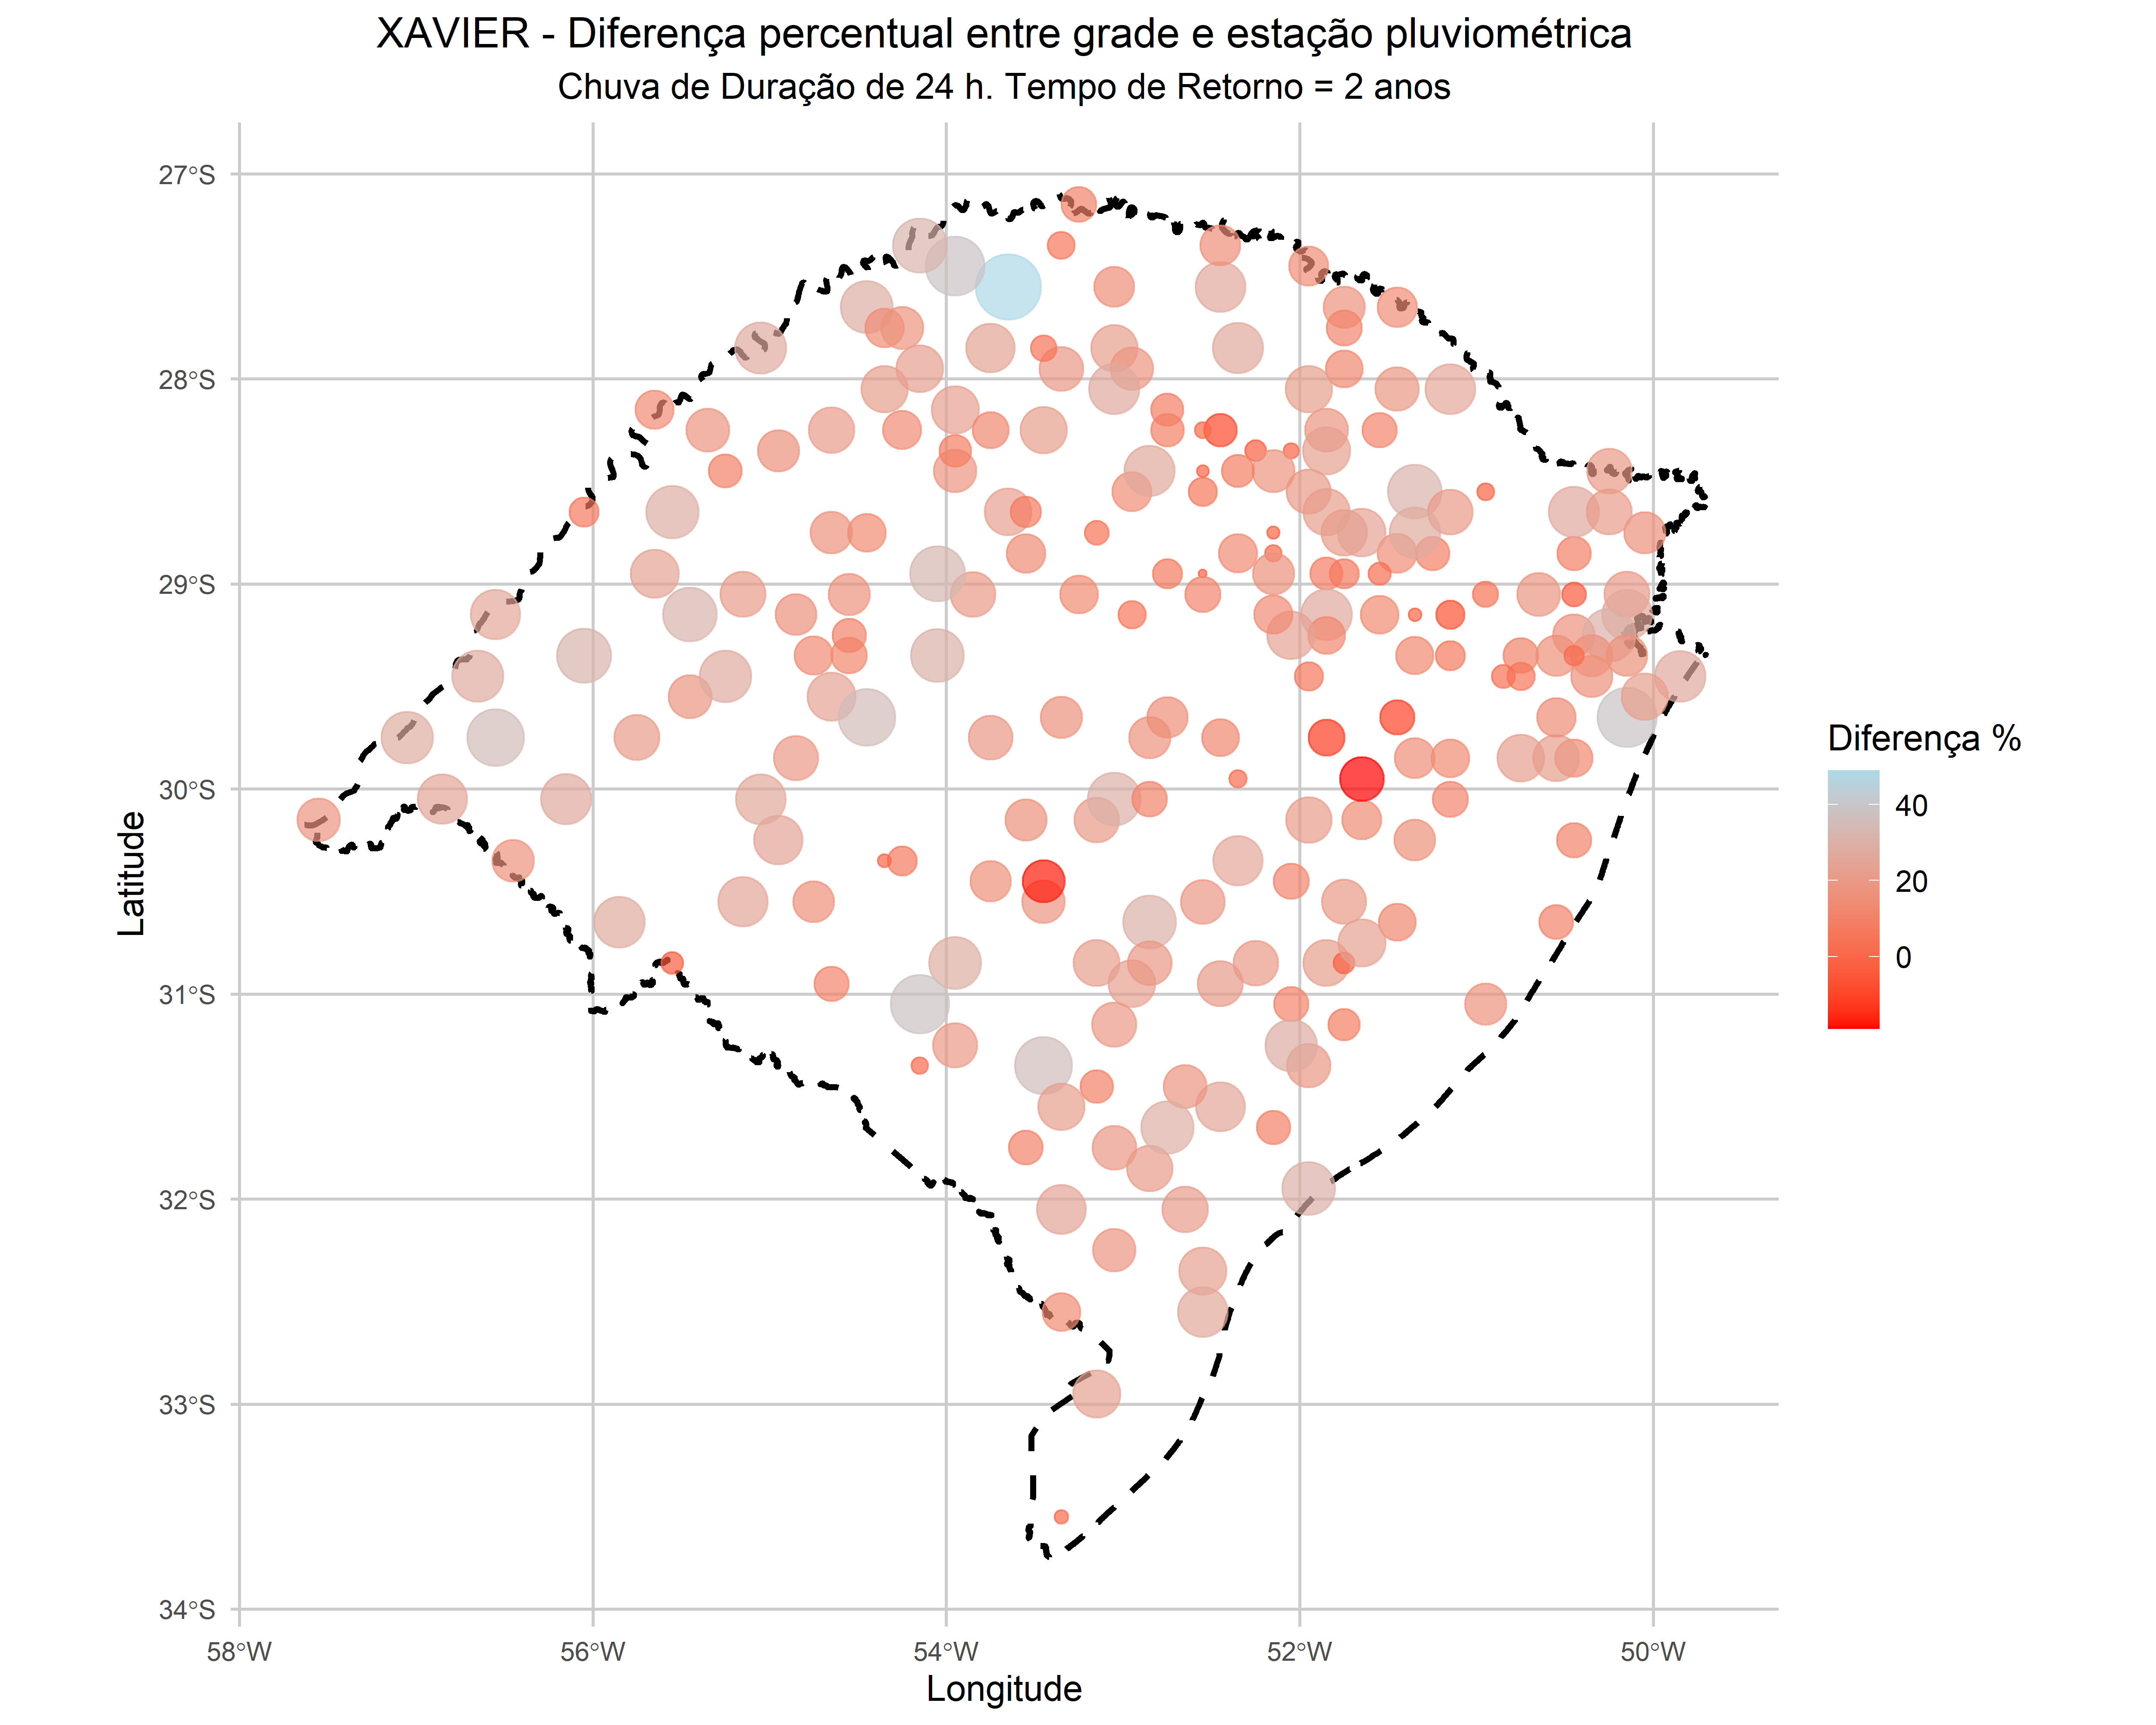
\includegraphics{Figuras/Figura21a.png}

}

\subcaption{\label{fig-Figura21a}XAVIER}

\end{minipage}%
\newline
\begin{minipage}{\linewidth}

\centering{

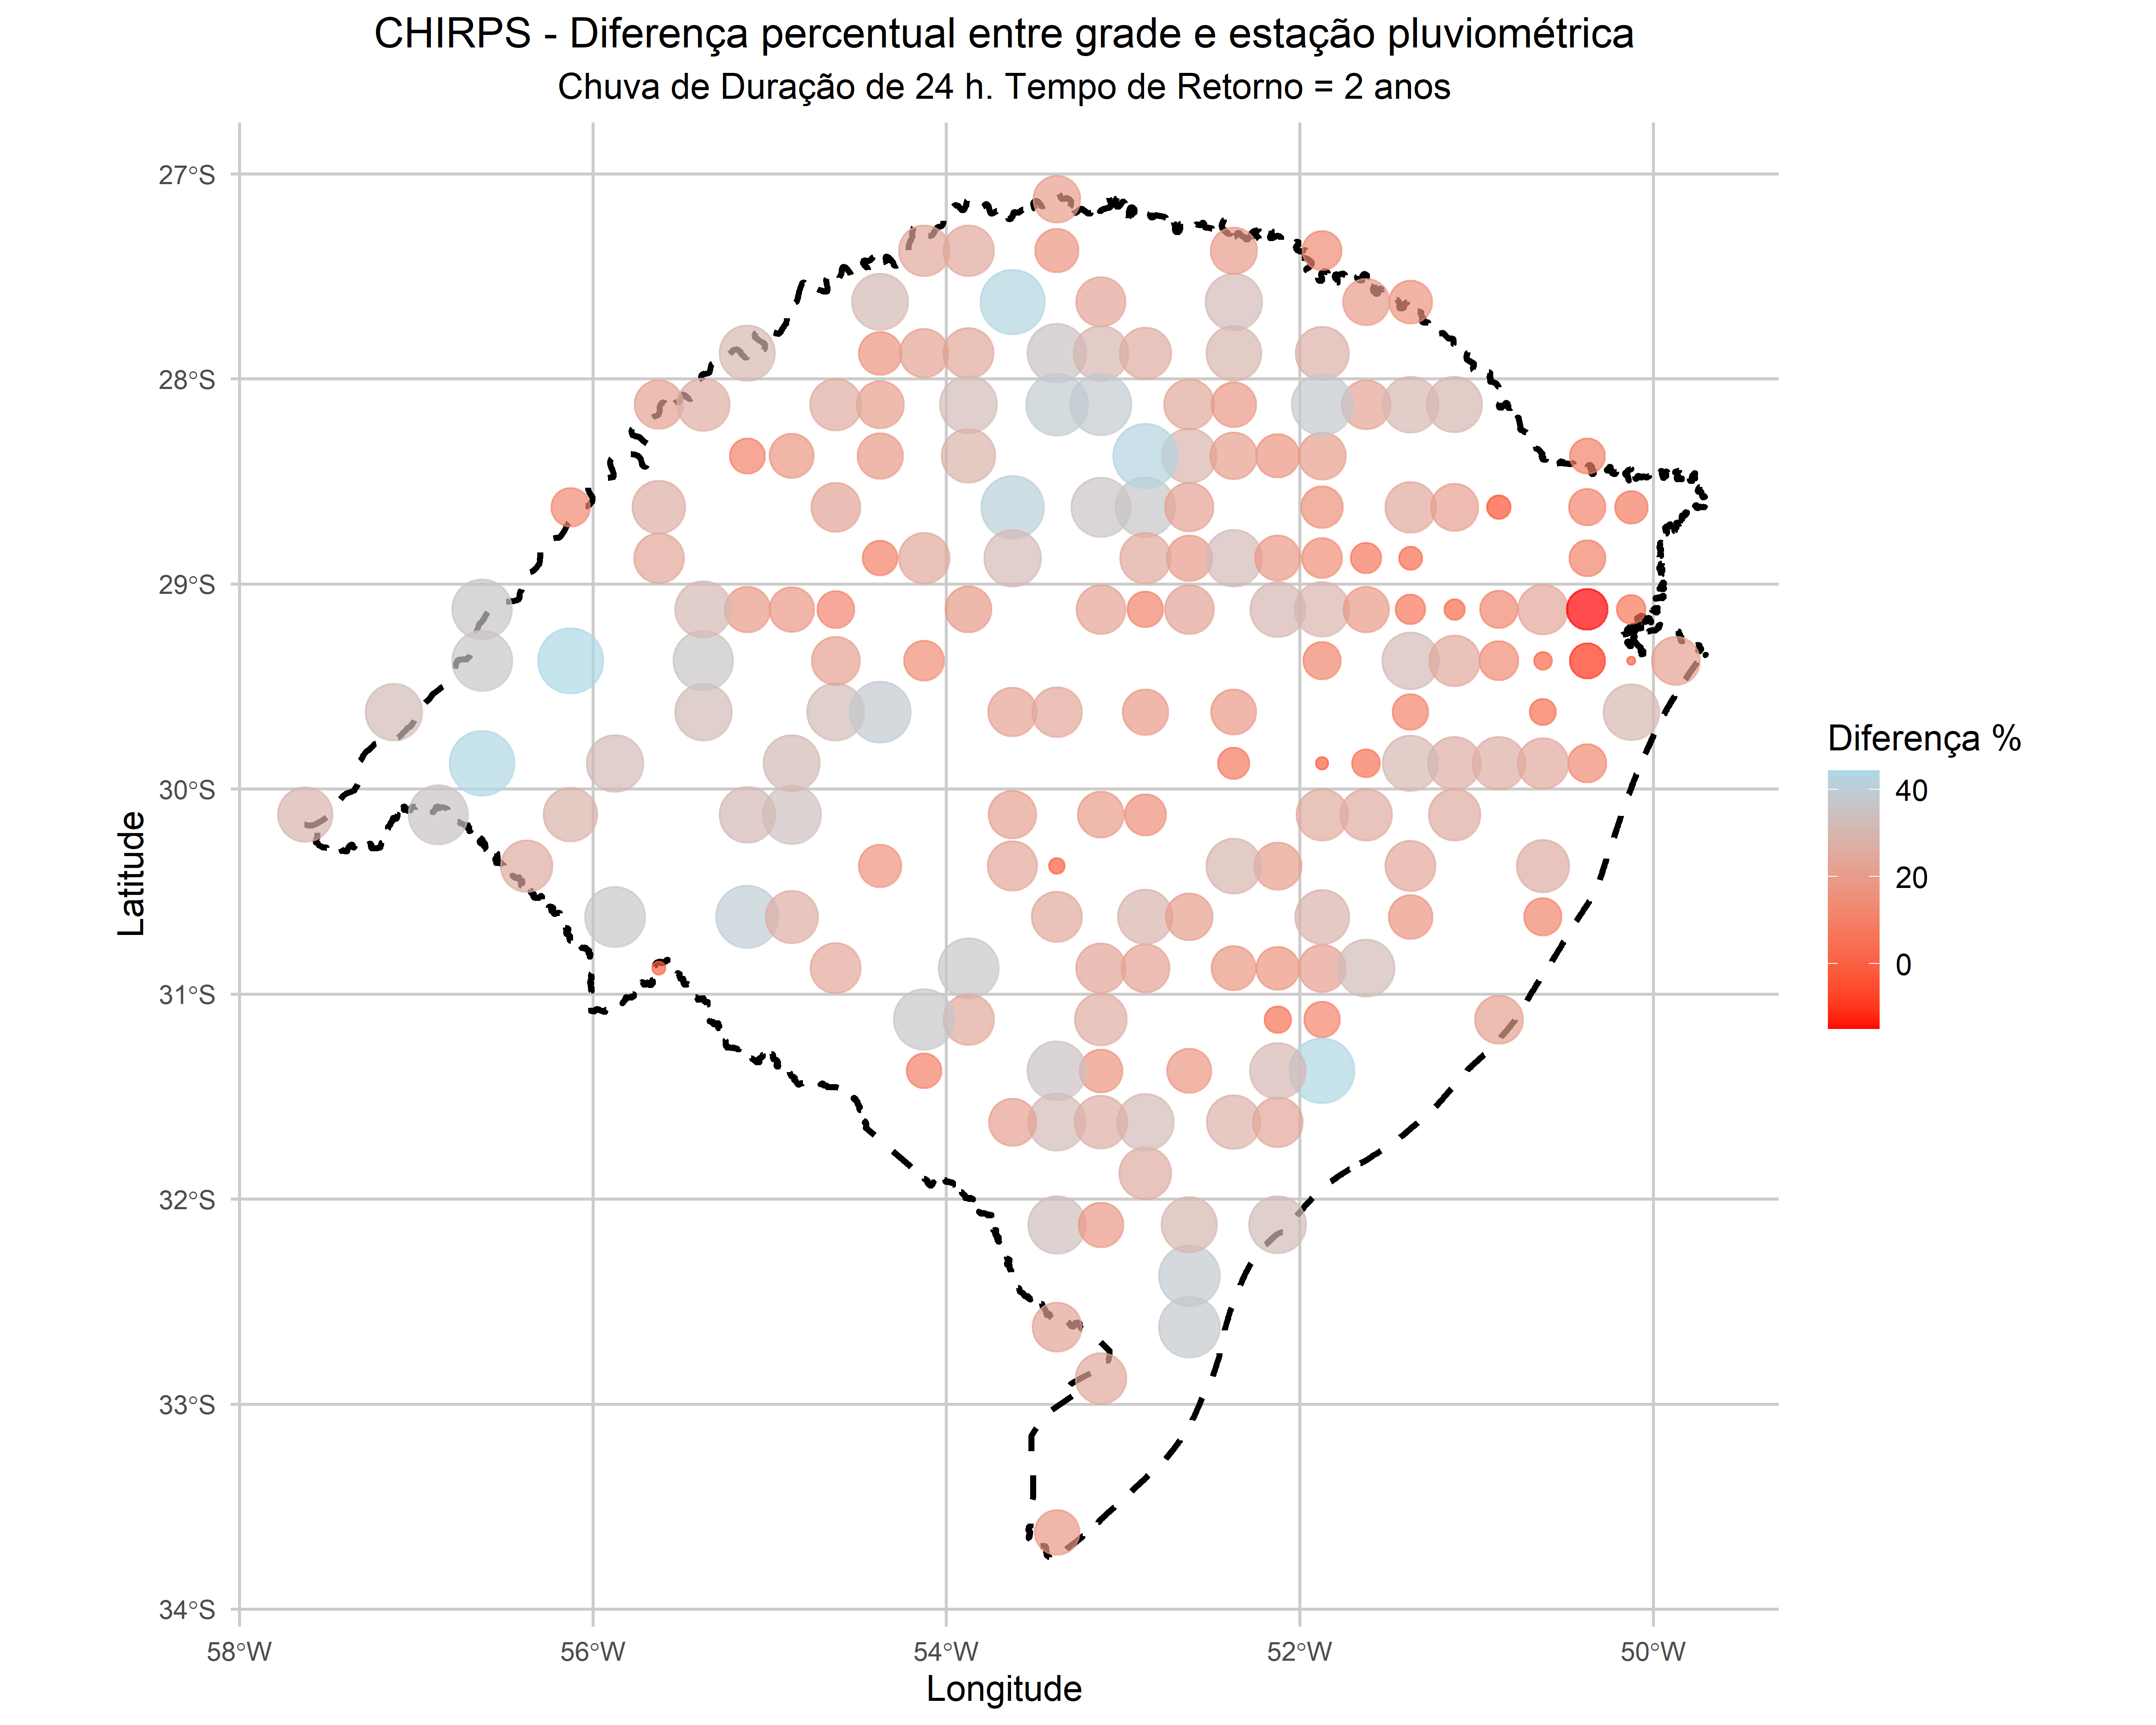
\includegraphics{Figuras/Figura21b.png}

}

\subcaption{\label{fig-Figura21b}CHIRPS}

\end{minipage}%

\caption{\label{fig-Figura21}Diferença percentual entre grade e estação
pluviométrica para a distribuição GEV-MME, com chuva de duração de 24
horas para tempo de retorno de 2 anos, considerando as bases XAVIER (a)
e CHIRPS (b).}

\end{figure}%

\begin{figure}

\begin{minipage}{\linewidth}

\centering{

\includegraphics{Figuras/Figura22a.png}

}

\subcaption{\label{fig-Figura22a}XAVIER}

\end{minipage}%
\newline
\begin{minipage}{\linewidth}

\centering{

\includegraphics{Figuras/Figura22b.png}

}

\subcaption{\label{fig-Figura22b}CHIRPS}

\end{minipage}%

\caption{\label{fig-Figura22}Diferença percentual entre grade e estação
pluviométrica para a distribuição GEV-MME, com chuva de duração de 24
horas para tempo de retorno de 5 anos, considerando as bases XAVIER (a)
e CHIRPS (b).}

\end{figure}%

\begin{figure}

\begin{minipage}{\linewidth}

\centering{

\includegraphics{Figuras/Figura23a.png}

}

\subcaption{\label{fig-Figura23a}XAVIER}

\end{minipage}%
\newline
\begin{minipage}{\linewidth}

\centering{

\includegraphics{Figuras/Figura23b.png}

}

\subcaption{\label{fig-Figura23b}CHIRPS}

\end{minipage}%

\caption{\label{fig-Figura23}Diferença percentual entre grade e estação
pluviométrica para a distribuição GEV-MME, com chuva de duração de 24
horas para tempo de retorno de 25 anos, considerando as bases XAVIER (a)
e CHIRPS (b).}

\end{figure}%

\begin{figure}

\begin{minipage}{\linewidth}

\includegraphics{Figuras/Figura24a.png}

\subcaption{\label{}XAVIER}
\end{minipage}%
\newline
\begin{minipage}{\linewidth}

\includegraphics{Figuras/Figura24b.png}

\subcaption{\label{}CHIRPS}
\end{minipage}%

\caption{\label{fig-Figura24}Diferença percentual entre grade e estação
pluviométrica para a distribuição GEV-MME, com chuva de duração de 24
horas para tempo de retorno de 100 anos, considerando as bases XAVIER
(a) e CHIRPS (b).}

\end{figure}%

\begin{figure}

\begin{minipage}{\linewidth}

\centering{

\includegraphics{Figuras/Figura25a.png}

}

\subcaption{\label{fig-Figura25a}XAVIER}

\end{minipage}%
\newline
\begin{minipage}{\linewidth}

\centering{

\includegraphics{Figuras/Figura25b.png}

}

\subcaption{\label{fig-Figura25b}CHIRPS}

\end{minipage}%

\caption{\label{fig-Figura25}Diferença percentual entre grade e estação
pluviométrica para a distribuição GEV-MME, com chuva de duração de 24
horas para tempo de retorno de 500 anos, considerando as bases XAVIER
(a) e CHIRPS (b).}

\end{figure}%

\begin{figure}

\begin{minipage}{\linewidth}

\centering{

\includegraphics{Figuras/Figura26a.png}

}

\subcaption{\label{fig-Figura26a}IDW}

\end{minipage}%
\newline
\begin{minipage}{\linewidth}

\centering{

\includegraphics{Figuras/Figura26b.png}

}

\subcaption{\label{fig-Figura26b}OK}

\end{minipage}%

\caption{\label{fig-Figura26}MAPE para cada local da estação para uma
chuva de duração de 24 horas para tempo de retorno de 2 anos,
considerando IDW (a) e OK (b).}

\end{figure}%

\begin{figure}

\begin{minipage}{\linewidth}

\centering{

\includegraphics{Figuras/Figura27a.png}

}

\subcaption{\label{fig-Figura27a}IDW}

\end{minipage}%
\newline
\begin{minipage}{\linewidth}

\centering{

\includegraphics{Figuras/Figura27b.png}

}

\subcaption{\label{fig-Figura27b}OK}

\end{minipage}%

\caption{\label{fig-Figura27}MAPE para cada local da estação para uma
chuva de duração de 24 horas para tempo de retorno de 5 anos,
considerando IDW (a) e OK (b).}

\end{figure}%

\begin{figure}

\begin{minipage}{\linewidth}

\centering{

\includegraphics{Figuras/Figura28a.png}

}

\subcaption{\label{fig-Figura28a}IDW}

\end{minipage}%
\newline
\begin{minipage}{\linewidth}

\centering{

\includegraphics{Figuras/Figura28b.png}

}

\subcaption{\label{fig-Figura28b}OK}

\end{minipage}%

\caption{\label{fig-Figura28}MAPE para cada local da estação para uma
chuva de duração de 24 horas para tempo de retorno de 25 anos,
considerando IDW (a) e OK (b).}

\end{figure}%

\begin{figure}

\begin{minipage}{\linewidth}

\centering{

\includegraphics{Figuras/Figura29a.png}

}

\subcaption{\label{fig-Figura29a}IDW}

\end{minipage}%
\newline
\begin{minipage}{\linewidth}

\centering{

\includegraphics{Figuras/Figura29b.png}

}

\subcaption{\label{fig-Figura29b}OK}

\end{minipage}%

\caption{\label{fig-Figura29}MAPE para cada local da estação para uma
chuva de duração de 24 horas para tempo de retorno de 100 anos,
considerando IDW (a) e OK (b).}

\end{figure}%

\begin{figure}

\begin{minipage}{\linewidth}

\centering{

\includegraphics{Figuras/Figura30a.png}

}

\subcaption{\label{fig-Figura30a}IDW}

\end{minipage}%
\newline
\begin{minipage}{\linewidth}

\centering{

\includegraphics{Figuras/Figura30b.png}

}

\subcaption{\label{fig-Figura30b}OK}

\end{minipage}%

\caption{\label{fig-Figura30}MAPE para cada local da estação para uma
chuva de duração de 24 horas para tempo de retorno de 500 anos,
considerando IDW (a) e OK (b).}

\end{figure}%

\subsection{Interpolação a partir dos parâmetros das
IDFs}\label{interpolauxe7uxe3o-a-partir-dos-paruxe2metros-das-idfs}

As Figuras 31 a 35 apresentam os resultados comparativos das
interpolações realizadas a partir dos parâmetros das IDFs por IDW e OK
para os diferentes tempos de retorno testados (2, 5, 25, 100 e 500
anos), respectivamente. Para cada figura dessa sequência são
apresentados os resultados da espacialização por IDW (a) e OK (b).

Comparando as Figuras 31 a 35 com as Figuras 10 a 14, verifica-se que as
diferenças entre interpolação dos quantis obtidos das estações para as
pontos de grade, ou a interpolação dos parãmetros das IDFs para os
pontos de grade para, em seguida, serem calculados os quantis de chuva
não representou diferença relevante.

\begin{figure}

\begin{minipage}{\linewidth}

\centering{

\includegraphics{Figuras/Figura31a.png}

}

\subcaption{\label{fig-Figura31a}Espacialização por IDW (p=2,5). Tempo
de Retorno =2 anos}

\end{minipage}%
\newline
\begin{minipage}{\linewidth}

\centering{

\includegraphics{Figuras/Figura31b.png}

}

\subcaption{\label{fig-Figura31b}Espacialização por OK. Tempo de Retorno
=2 anos}

\end{minipage}%

\caption{\label{fig-Figura31}Resultados obtidos para intensidade da
chuva de duração de 24 h e tempo de retorno de 2 anos para interpolação
por IDW dos parâmetros das IDFs (a) e por krigagem ordinária, OK (b).}

\end{figure}%

\begin{figure}

\begin{minipage}{\linewidth}

\centering{

\includegraphics{Figuras/Figura32a.png}

}

\subcaption{\label{fig-Figura32a}Espacialização por IDW (p=2.5). Tempo
de Retorno =5 anos}

\end{minipage}%
\newline
\begin{minipage}{\linewidth}

\centering{

\includegraphics{Figuras/Figura32b.png}

}

\subcaption{\label{fig-Figura32b}Espacialização por OK. Tempo de Retorno
=5 anos}

\end{minipage}%

\caption{\label{fig-Figura32}Resultados obtidos para intensidade da
chuva de duração de 24 h e tempo de retorno de 5 anos para interpolação
por IDW dos parâmetros das IDFs (a) e por krigagem ordinária, OK (b).}

\end{figure}%

\begin{figure}

\begin{minipage}{\linewidth}

\centering{

\includegraphics{Figuras/Figura33a.png}

}

\subcaption{\label{fig-Figura33a}Espacialização por IDW (p=2). Tempo de
Retorno =25 anos}

\end{minipage}%
\newline
\begin{minipage}{\linewidth}

\centering{

\includegraphics{Figuras/Figura33b.png}

}

\subcaption{\label{fig-Figura33b}Espacialização por OK. Tempo de Retorno
=25 anos}

\end{minipage}%

\caption{\label{fig-Figura33}Resultados obtidos para intensidade da
chuva de duração de 24 h e tempo de retorno de 25 anos para interpolação
por IDW dos parâmetros das IDFs (a) e por krigagem ordinária, OK (b).}

\end{figure}%

\begin{figure}

\begin{minipage}{\linewidth}

\centering{

\includegraphics{Figuras/Figura34a.png}

}

\subcaption{\label{fig-Figura34a}Espacialização por IDW (p=1). Tempo de
Retorno =100 anos}

\end{minipage}%
\newline
\begin{minipage}{\linewidth}

\centering{

\includegraphics{Figuras/Figura34b.png}

}

\subcaption{\label{fig-Figura34b}Espacialização por OK. Tempo de Retorno
=100 anos}

\end{minipage}%

\caption{\label{fig-Figura34}Resultados obtidos para intensidade da
chuva de duração de 24 h e tempo de retorno de 100 anos para
interpolação por IDW dos parâmetros das IDFs (a) e por krigagem
ordinária, OK (b).}

\end{figure}%

\begin{figure}

\begin{minipage}{\linewidth}

\centering{

\includegraphics{Figuras/Figura35a.png}

}

\subcaption{\label{fig-Figura35a}Espacialização por IDW (p=0.5). Tempo
de Retorno =500 anos}

\end{minipage}%
\newline
\begin{minipage}{\linewidth}

\centering{

\includegraphics{Figuras/Figura35b.png}

}

\subcaption{\label{fig-Figura35b}Espacialização por OK. Tempo de Retorno
=500 anos}

\end{minipage}%

\caption{\label{fig-Figura35}Resultados obtidos para intensidade da
chuva de duração de 24 h e tempo de retorno de 500 anos para
interpolação por IDW dos parâmetros das IDFs (a) e por krigagem
ordinária, OK (b).}

\end{figure}%

\subsection{IDFs para os municípios}\label{idfs-para-os-municuxedpios}

A partir da interpolação por IDW dos parâmetros das curvas IDFs das
estações foram geradas curvas IDFs para todas as sedes municipais do Rio
Grande do Sul. Para interpolação, foram adotados os expoentes de melhor
desempenho e a distribuição GEV, com parâmetros definidos pelo método
MML. O aplicativo a seguir permite a seleção da sede municipal e a
geração das curvas IDFs, sendo possível visualizar a equação, bem como
os resultados na forma de tabelas.

\section{Conclusões}\label{conclusuxf5es}

Este estudo comparou e analisou a espacialização dos dados provenientes
das estações pluviométricas da base HIDRO com os dados de precipitação
em grade fornecidos pelas bases XAVIER e CHIRPS, amplamente utilizadas
no Brasil. Os resultados dos padrões de chuvas extremas, obtidos por
meio das equações IDFs das estações pluviométricas da base HIDRO, foram
comparados com aqueles derivados das bases em grade.

A análise, realizada para o estado do Rio Grande do Sul, revelou
diferenças significativas nos quantis de chuva das curvas IDFs, com
dados interpolados utilizando os métodos IDW e Krigagem, considerando
diferentes distribuições de máximos (Gumbel, GEV e Exponencial) e
técnicas para obtenção de parâmetros na análise de frequência. As
incertezas entre as distribuições de extremos foram avaliadas, e as
curvas IDFs foram interpoladas para todas as sedes municipais do estado.
Os resultados indicam que os dados em grade tendem a subestimar os
quantis de chuva, sugerindo a necessidade de uma análise cuidadosa ao
utilizar esses dados para o dimensionamento de infraestruturas hídricas.

\section*{Referências}\label{referuxeancias}
\addcontentsline{toc}{section}{Referências}

\phantomsection\label{refs}
\begin{CSLReferences}{1}{0}
\vspace{1em}

\bibitem[\citeproctext]{ref-ASCE1992}
American Society of Civil Engineers. (1992). \emph{Design and
construction of urban stormwater systems}. New York: American Society of
Civil Engineers.

\bibitem[\citeproctext]{ref-Aghakouchak2013}
Amir, A., David, E., Kuolin, H., Siegfried, S., \& Soroosh, S. (Eds.).
(2013). \emph{Extremes in a changing climate. Detection, analysis and
uncertainty}. Rio de Janeiro RJ: Springer Dordrecht.
https://doi.org/\url{https://doi.org/10.1007/978-94-007-4479-0}

\bibitem[\citeproctext]{ref-ANA2007}
ANA. (2007). \emph{Evolução da rede hidrometeorológica nacional.} (No.
v.1.n.1). Brasilia, DF: Superintendência de Administração da Rede
Hidrometeorológica. Retrieved from
\url{https://www.ana.gov.br/arquivos/infohidrologicas/EvolucaodaRedeHidrometeorologicaNacional.pdf}

\bibitem[\citeproctext]{ref-ANA2019}
ANA. (2019). Portal hidroweb. Retrieved from
\url{http://www.snirh.gov.br/hidroweb/publico/apresentacao.jsf}

\bibitem[\citeproctext]{ref-Asadieh2015}
Asadieh, B., \& Krakauer, N. Y. (2015). Global trends in extreme
precipitation: Climate models versus observations. \emph{Hydrology and
Earth System Sciences}, \emph{19}(2), 877--891.
\url{https://doi.org/10.5194/hess-19-877-2015}

\bibitem[\citeproctext]{ref-bemfica2000}
Bemfica, D. C., Goldenfum, J. A., \& Silveira, A. L. L. (2000). Análise
da aplicabilidade de padrões de chuva de projeto a porto alegre.
\emph{Revista Brasileira de Recursos Hídricos}, \emph{5}(4), 5--16.

\bibitem[\citeproctext]{ref-bertoni1993}
Bertoni, J. C., \& Tucci, C. E. M. (1993). Precipitação. In C. E. M.
Tucci (Ed.), \emph{Hidrologia: Ciência e aplicação} (pp. 177--241).
Porto Alegre: Editora da UFRGS.

\bibitem[\citeproctext]{ref-bravo2008}
Bravo, J. M., Tucci, C. E. M., Tassi, R., \& Allasia, D. (2008).
Regionalização de curvas intensidade, duração e frequência de
precipitação: Aplicação do distrito federal. In \emph{Anais do II
simpósio de recursos hídricos do sul sudeste} (p. --). Rio de Janeiro.

\bibitem[\citeproctext]{ref-Burnham2002}
Burnham, K. P., \& Anderson, D. R. (2002). \emph{Model selection and
multimodel inference: A practical information-theoretic approach}. New
York: Springer.

\bibitem[\citeproctext]{ref-casella2002statistical}
Casella, G., \& Berger, R. L. (2002). \emph{Statistical inference}.
Pacific Grove, CA: Duxbury Press.

\bibitem[\citeproctext]{ref-Chambers1992}
Chambers, J. M., \& Hastie, T. J. (1992). \emph{Statistical models}. New
York: Wiley.

\bibitem[\citeproctext]{ref-Cohen1992}
Cohen, J. (1992). \emph{A power primer}. \emph{Psychological Bulletin}
(Vol. 112, pp. 155--159). American Psychological Association.

\bibitem[\citeproctext]{ref-cox1961analysis}
Cox, D. R., \& Hinkley, D. V. (1961). \emph{The analysis of binary
data}. London: Chapman \& Hall.

\bibitem[\citeproctext]{ref-DAEE1980}
DAE, \& CETESB. (1980). \emph{Drenagem urbana, manual de projeto}. São
Paulo: Departamento de Águas e Energia Elétrica e Companhia de
Tecnologia de Saneamento.

\bibitem[\citeproctext]{ref-distrito_federal2009}
Distrito Federal. (2009). \emph{Plano diretor de drenagem urbana do
distrito federal: Relatório de produto 4} (No. Tomo 01/07) (Vol. 8, p.
104). Brasília: Secretaria de Estado de Obras; Concremat Engenharia.

\bibitem[\citeproctext]{ref-Eletrobras1987}
ELETROBRAS. (1987). \emph{Guia para cálculo de cheia de projeto de
vertedouros} (p. 215). Rio de Janeiro: Eletrobrás.

\bibitem[\citeproctext]{ref-fragoso2004}
Fragoso Jr., C. R. (2004). Regionalização da vazão máxima instantânea
com base na precipitação de projeto. \emph{ReRH: Revista Eletrônica de
Recursos Hídricos}, \emph{1}(1), 5--13.

\bibitem[\citeproctext]{ref-ImpactOfClimateChange2024}
Fung, I., Leung, L. R., \& Eltahir, E. A. B. (Eds.). (2024).
\emph{Impact of climate change on water resources: Modeling techniques
and case studies}. Cham: Springer.

\bibitem[\citeproctext]{ref-funk2015}
Funk, C., Peterson, P., Landsfeld, M., Pedreros, D., Verdin, J., Shukla,
S., et al. (2015). The climate hazards InfraRed precipitation with
stations---a new environmental record for monitoring extremes.
\emph{Scientific Data}, \emph{2}, 150066.
\url{https://doi.org/10.1038/sdata.2015.66}

\bibitem[\citeproctext]{ref-Gao2014}
Gao, H., Li, L., \& Li, X. (2014). Evaluation of climate model
performance and its impact on hydrological simulations in a mountain
watershed. \emph{Journal of Hydrology}, \emph{510}, 52--63.

\bibitem[\citeproctext]{ref-Giorgi2002}
Giorgi, F., \& Mearns, L. O. (2002). Calculation of average, uncertainty
range, and reliability of regional climate change scenarios.
\emph{Climate Research}, \emph{22}, 197--207.

\bibitem[\citeproctext]{ref-Giorgi2004}
Giorgi, F., \& Mearns, L. O. (2004). Climate change scenarios for the
21st century: Implications for regional climate impacts. \emph{Climate
Change}, \emph{60}, 287--316.
\url{https://doi.org/10.1023/B:CLIM.0000018552.40082.3b}

\bibitem[\citeproctext]{ref-goncalves2011}
Gonçalves, L. S. (2011). \emph{Relações intensidade-duração-frequência
com base em estimativas de precipitação por satélite} (Dissertação de
Mestrado). Universidade Federal do Rio Grande do Sul, Programa de
Pós-Graduação em Recursos Hídricos e Saneamento Ambiental. Retrieved
from \url{https://lume.ufrgs.br/handle/10183/49152}

\bibitem[\citeproctext]{ref-Gravata2024}
Gravatal, R. S. (2024). \emph{Determinação das equações de chuvas
intensivas para o estado de rondônia} (Dissertação de Mestrado).
PROFÁGUA -- Mestrado Profissional em Rede Nacional em Gestão e Regulação
dos Recursos Hídricos, Brasil.

\bibitem[\citeproctext]{ref-Gudmundsson2012}
Gudmundsson, L., Seneviratne, S. I., \& St. Jacques, J. M. (2012). The
role of data quality in evaluating climate model performance.
\emph{Geophysical Research Letters}, \emph{39}, L21701.

\bibitem[\citeproctext]{ref-hansen1982generalized}
Hansen, L. P., \& Singleton, K. J. (1982). Generalized instrumental
variables estimation of nonlinear rational expectations models.
\emph{Econometrica}, \emph{50}(5), 1269--1286. Retrieved from
\url{https://www.jstor.org/stable/1912775}

\bibitem[\citeproctext]{ref-hinkley1995generalized}
Hinkley, D. V., \& Lee, S. J. R. (1995). Generalized moment estimation
and other methods. \emph{Journal of Statistical Planning and Inference},
\emph{45}(1), 47--64. Retrieved from
\url{https://doi.org/10.1016/0378-3758(94)00054-D}

\bibitem[\citeproctext]{ref-Huffman2001}
Huffman, G. J., Adler, R. F., Bolvin, D. T., Gu, G., Nelkin, E. J., \&
Bowman, K. P. (2001). Global precipitation at one-degree daily
resolution from multi-satellite observations. \emph{Journal of
Hydrometeorology}, \emph{2}(1), 36--50.
\url{https://doi.org/10.1175/1525-7541(2001)002\%3C0036:GPADOW\%3E2.0.CO;2}

\bibitem[\citeproctext]{ref-Hughes2013}
Hughes, J. K., Hay, L. E., \& Wilby, R. L. (2013). Evaluation of climate
model outputs for hydrological impact assessments in the u.s.
\emph{Journal of Hydrology}, \emph{482}, 151--163.

\bibitem[\citeproctext]{ref-johnson1994systems}
Johnson, N. L., \& Kotz, S. (1994). Systems of frequency curves.
\emph{Journal of the American Statistical Association}, \emph{89}(425),
1626--1634. Retrieved from \url{https://www.jstor.org/stable/2290627}

\bibitem[\citeproctext]{ref-jorgensen1997theory}
Jørgensen, B. (1997). The theory of sampling. \emph{Journal of the Royal
Statistical Society: Series B (Methodological)}, \emph{59}(2), 235--252.
Retrieved from
\url{https://onlinelibrary.wiley.com/doi/10.1111/1467-9868.00082}

\bibitem[\citeproctext]{ref-Kolmogorov1933}
Kolmogorov, A. (1933). Sulla determinazione empirica di una legge di
distribuzione. \emph{Giornale Dell'Istituto Italiano Degli Attuari},
\emph{4}, 83--99.

\bibitem[\citeproctext]{ref-Li2014}
Li, W., Zhang, Z., \& Sun, J. (2014). Evaluation of climate models for
regional climate projections and hydrological impact assessments.
\emph{International Journal of Climatology}, \emph{34}, 1025--1040.

\bibitem[\citeproctext]{ref-macdonald2009hidden}
MacDonald, I. L., \& Zucchini, W. (2009). Hidden markov models and other
statistical models with algorithms and applications. \emph{Journal of
the Royal Statistical Society: Series B (Statistical Methodology)},
\emph{71}(1), 113--128. Retrieved from
\url{https://onlinelibrary.wiley.com/doi/abs/10.1111/j.1467-9868.2008.00712.x}

\bibitem[\citeproctext]{ref-Matheron1963}
Matheron, G. (1963). Principles of geostatistics. \emph{Economic
Geology}, \emph{58}(8), 1246--1266.

\bibitem[\citeproctext]{ref-mcdonald2018impact}
McDonald, C. S., Lee, S. M., \& Smith, J. C. (2018). The impact of grid
resolution on the simulation of extreme precipitation events.
\emph{Journal of Hydrometeorology}, \emph{19}(6), 1023--1040.
\url{https://doi.org/10.1175/JHM-D-17-0201.1}

\bibitem[\citeproctext]{ref-Milly2008}
Milly, P. C., Betancourt, J., Falkenmark, M., Hirsch, R. M., Kundzewicz,
Z. W., Lettenmaier, D. P., \& Stouffer, R. J. (2008). Stationarity is
dead: Whither water management? \emph{Science}, \emph{319}(5863).
\url{https://doi.org/10.1126/science.1151915}

\bibitem[\citeproctext]{ref-morrison1994comparison}
Morrison, D. F., \& Tang, W. M. K. (1994). Comparison of estimation
methods for small samples. \emph{Journal of the American Statistical
Association}, \emph{89}(425), 1105--1112. Retrieved from
\url{https://www.jstor.org/stable/2290698}

\bibitem[\citeproctext]{ref-New2001}
New, M., Hulme, M., \& Jones, P. (2001). Representing twentieth-century
space-time climate variability. Part i: Development of a 1961--1990 mean
monthly terrestrial climatology. \emph{Journal of Climate}, \emph{14},
834--852.

\bibitem[\citeproctext]{ref-Pearson1900}
Pearson, K. (1900). X. On the criterion that a given system of
deviations from the probable in the case of a correlation is likely to
have arisen from random sampling. \emph{Philosophical Magazine},
\emph{50}(302), 157--175.

\bibitem[\citeproctext]{ref-Pfafstetter1957}
Pfafstetter, O. (1957). \emph{Chuvas intensas no brasil, relação entre
precipitação, duração e frequência de chuvas em 98 postos com
pluviógrafos}. Rio de Janeiro RJ: Departamento Nacional de Obras de
Saneamento.

\bibitem[\citeproctext]{ref-porto1995escoamento}
Porto, R. L. (1995). Escoamento superficial direto. In C. E. M. Tucci,
R. L. Porto, \& M. T. L. Barros (Eds.), \emph{Drenagem urbana} (pp.
xx--yy). Porto Alegre: ABRH/Editora da Universidade/UFRGS.

\bibitem[\citeproctext]{ref-RaoHamed2000}
Rao, A. R., \& Hamed, K. H. (2000). \emph{Flood frequency analysis}.
Florida, USA: CRC Press LLC.

\bibitem[\citeproctext]{ref-R}
R-Core-Team. (2023). \emph{R: A language and environment for statistical
computing}. Vienna, Austria: R Foundation for Statistical Computing.
Retrieved from \url{https://www.R-project.org/}

\bibitem[\citeproctext]{ref-Semenov2008}
Semenov, M. A., \& Barrow, E. M. (2008). A process-based approach for
estimating the effects of climate change on crop yields. \emph{Climate
Research}, \emph{37}, 213--223. \url{https://doi.org/10.3354/cr00771}

\bibitem[\citeproctext]{ref-Shepard1968}
Shepard, D. W. (1968). A two-dimensional interpolation function for
irregularly-spaced data. \emph{Proceedings of the 1968 23rd ACM National
Conference}, 517--524.

\bibitem[\citeproctext]{ref-Sillmann2013}
Sillmann, J., Kharin, V. V., \& Zwiers, F. W. (2013). Climate extremes
indices in the CMIP5 multimodel ensemble. \emph{Journal of Geophysical
Research: Atmospheres}, \emph{118}, 4714--4736.

\bibitem[\citeproctext]{ref-Smirnov1948}
Smirnov, N. (1948). Estimation of the discrepancy between empirical and
theoretical distributions. \emph{Bulletin of Moscow University, Series
A}, \emph{2}, 3--14.

\bibitem[\citeproctext]{ref-Tucci2004}
Tucci, C. E. M. (2004). \emph{Hidrologia: Ciência e aplicação} (p. 943).
Porto Alegre: UFRGS; ABRH.

\bibitem[\citeproctext]{ref-xavier2015}
Xavier, A., King, W., \& Scanlon, B. (2015). Daily gridded
meteorological variables in brazil (1980--2013). \emph{International
Journal of Climatology}, \emph{36}, 2644--2659.
\url{https://doi.org/10.1002/joc.4518}

\bibitem[\citeproctext]{ref-xavier2017}
Xavier, A., King, C., \& Scanlon, B. (2017). An update of xavier, king
and scanlon (2016) daily precipitation gridded data set for brazil. In
\emph{Conference proceedings} (pp. 562--569). Retrieved from
\url{https://proceedings.science/sbsr/papers/an-update-of-xavier--king-and-scanlon--2016--daily-precipitation-gridded-data-set-for-the-brazil}

\end{CSLReferences}




\end{document}
